\documentclass[twoside]{article}

% Packages required by doxygen
\usepackage{fixltx2e}
\usepackage{calc}
\usepackage{doxygen}
\usepackage[export]{adjustbox} % also loads graphicx
\usepackage{graphicx}
\usepackage[utf8]{inputenc}
\usepackage{makeidx}
\usepackage{multicol}
\usepackage{multirow}
\PassOptionsToPackage{warn}{textcomp}
\usepackage{textcomp}
\usepackage[nointegrals]{wasysym}
\usepackage[table]{xcolor}

% NLS support packages
\usepackage[danish]{babel}
\usepackage[T1]{fontenc}

% Font selection
\usepackage[T1]{fontenc}
\usepackage[scaled=.90]{helvet}
\usepackage{courier}
\usepackage{amssymb}
\usepackage{sectsty}
\renewcommand{\familydefault}{\sfdefault}
\allsectionsfont{%
  \fontseries{bc}\selectfont%
  \color{darkgray}%
}
\renewcommand{\DoxyLabelFont}{%
  \fontseries{bc}\selectfont%
  \color{darkgray}%
}
\newcommand{\+}{\discretionary{\mbox{\scriptsize$\hookleftarrow$}}{}{}}

% Page & text layout
\usepackage{geometry}
\geometry{%
  a4paper,%
  top=2.5cm,%
  bottom=2.5cm,%
  left=2.5cm,%
  right=2.5cm%
}
\tolerance=750
\hfuzz=15pt
\hbadness=750
\setlength{\emergencystretch}{15pt}
\setlength{\parindent}{0cm}
\setlength{\parskip}{3ex plus 2ex minus 2ex}
\makeatletter
\renewcommand{\paragraph}{%
  \@startsection{paragraph}{4}{0ex}{-1.0ex}{1.0ex}{%
    \normalfont\normalsize\bfseries\SS@parafont%
  }%
}
\renewcommand{\subparagraph}{%
  \@startsection{subparagraph}{5}{0ex}{-1.0ex}{1.0ex}{%
    \normalfont\normalsize\bfseries\SS@subparafont%
  }%
}
\makeatother

% Headers & footers
\usepackage{fancyhdr}
\pagestyle{fancyplain}
\fancyhead[LE]{\fancyplain{}{\bfseries\thepage}}
\fancyhead[CE]{\fancyplain{}{}}
\fancyhead[RE]{\fancyplain{}{\bfseries\leftmark}}
\fancyhead[LO]{\fancyplain{}{\bfseries\rightmark}}
\fancyhead[CO]{\fancyplain{}{}}
\fancyhead[RO]{\fancyplain{}{\bfseries\thepage}}
\fancyfoot[LE]{\fancyplain{}{}}
\fancyfoot[CE]{\fancyplain{}{}}
\fancyfoot[RE]{\fancyplain{}{\bfseries\scriptsize Genereret af Doxygen }}
\fancyfoot[LO]{\fancyplain{}{\bfseries\scriptsize Genereret af Doxygen }}
\fancyfoot[CO]{\fancyplain{}{}}
\fancyfoot[RO]{\fancyplain{}{}}
\renewcommand{\footrulewidth}{0.4pt}
\renewcommand{\sectionmark}[1]{%
  \markright{\thesection\ #1}%
}

% Indices & bibliography
\usepackage{natbib}
\usepackage[titles]{tocloft}
\setcounter{tocdepth}{3}
\setcounter{secnumdepth}{5}
\makeindex

% Hyperlinks (required, but should be loaded last)
\usepackage{ifpdf}
\ifpdf
  \usepackage[pdftex,pagebackref=true]{hyperref}
\else
  \usepackage[ps2pdf,pagebackref=true]{hyperref}
\fi
\hypersetup{%
  colorlinks=true,%
  linkcolor=blue,%
  citecolor=blue,%
  unicode%
}

% Custom commands
\newcommand{\clearemptydoublepage}{%
  \newpage{\pagestyle{empty}\cleardoublepage}%
}

\usepackage{caption}
\captionsetup{labelsep=space,justification=centering,font={bf},singlelinecheck=off,skip=4pt,position=top}

%===== C O N T E N T S =====

\begin{document}

% Titlepage & ToC
\hypersetup{pageanchor=false,
             bookmarksnumbered=true,
             pdfencoding=unicode
            }
\pagenumbering{roman}
\begin{titlepage}
\vspace*{7cm}
\begin{center}%
{\Large L.\+A.\+M.\+P }\\
\vspace*{1cm}
{\large Genereret af Doxygen 1.8.11}\\
\end{center}
\end{titlepage}
\tableofcontents
\pagenumbering{arabic}
\hypersetup{pageanchor=true}

%--- Begin generated contents ---
\section{Modul-\/indeks}
\subsection{Moduler}
Her er en liste over alle moduler\+:\begin{DoxyCompactList}
\item \contentsline{section}{Length constant}{\pageref{group___m_a_x_l_e_n}}{}
\end{DoxyCompactList}

\section{Namespace-\/indeks}
\subsection{Oversigt over namespaces}
Her er en liste over alle namespaces med korte beskrivelser\+:\begin{DoxyCompactList}
\item\contentsline{section}{\hyperlink{namespace_ui}{Ui} }{\pageref{namespace_ui}}{}
\end{DoxyCompactList}

\section{Hierarkisk indeks}
\subsection{Klassehierarki}
Denne nedarvningsliste er sorteret næsten -\/ men ikke nødvendigvis helt -\/ alfabetisk\+:\begin{DoxyCompactList}
\item \contentsline{section}{Q\+Dialog}{\pageref{class_q_dialog}}{}
\begin{DoxyCompactList}
\item \contentsline{section}{Planner\+Dialog}{\pageref{class_planner_dialog}}{}
\end{DoxyCompactList}
\item \contentsline{section}{Q\+Tab\+Widget}{\pageref{class_q_tab_widget}}{}
\begin{DoxyCompactList}
\item \contentsline{section}{E3\+P\+JR}{\pageref{class_e3_p_j_r}}{}
\end{DoxyCompactList}
\item \contentsline{section}{Q\+Widget}{\pageref{class_q_widget}}{}
\begin{DoxyCompactList}
\item \contentsline{section}{Light}{\pageref{class_light}}{}
\item \contentsline{section}{Main\+Display}{\pageref{class_main_display}}{}
\item \contentsline{section}{Planner}{\pageref{class_planner}}{}
\item \contentsline{section}{Q\+Virtual\+Keyboard}{\pageref{class_q_virtual_keyboard}}{}
\item \contentsline{section}{Spi\+Test\+Program}{\pageref{class_spi_test_program}}{}
\end{DoxyCompactList}
\item \contentsline{section}{S\+P\+Iapi}{\pageref{class_s_p_iapi}}{}
\item \contentsline{section}{Ui\+\_\+\+E3\+P\+JR}{\pageref{class_ui___e3_p_j_r}}{}
\begin{DoxyCompactList}
\item \contentsline{section}{E3\+P\+JR}{\pageref{class_ui_1_1_e3_p_j_r}}{}
\end{DoxyCompactList}
\item \contentsline{section}{Ui\+\_\+\+Spi\+Test\+Program}{\pageref{class_ui___spi_test_program}}{}
\begin{DoxyCompactList}
\item \contentsline{section}{Spi\+Test\+Program}{\pageref{class_ui_1_1_spi_test_program}}{}
\end{DoxyCompactList}
\end{DoxyCompactList}

\section{Indeks over datastrukturer}
\subsection{Datastrukturer}
Her er datastrukturerne med korte beskrivelser\+:\begin{DoxyCompactList}
\item\contentsline{section}{\hyperlink{class_e3_p_j_r}{E3\+P\+JR} }{\pageref{class_e3_p_j_r}}{}
\item\contentsline{section}{\hyperlink{class_ui_1_1_e3_p_j_r}{E3\+P\+JR} }{\pageref{class_ui_1_1_e3_p_j_r}}{}
\item\contentsline{section}{\hyperlink{class_light}{Light} }{\pageref{class_light}}{}
\item\contentsline{section}{\hyperlink{class_main_display}{Main\+Display} }{\pageref{class_main_display}}{}
\item\contentsline{section}{\hyperlink{class_planner}{Planner} }{\pageref{class_planner}}{}
\item\contentsline{section}{\hyperlink{class_planner_dialog}{Planner\+Dialog} }{\pageref{class_planner_dialog}}{}
\item\contentsline{section}{\hyperlink{class_q_dialog}{Q\+Dialog} }{\pageref{class_q_dialog}}{}
\item\contentsline{section}{\hyperlink{class_q_tab_widget}{Q\+Tab\+Widget} }{\pageref{class_q_tab_widget}}{}
\item\contentsline{section}{\hyperlink{class_q_virtual_keyboard}{Q\+Virtual\+Keyboard} }{\pageref{class_q_virtual_keyboard}}{}
\item\contentsline{section}{\hyperlink{class_q_widget}{Q\+Widget} }{\pageref{class_q_widget}}{}
\item\contentsline{section}{\hyperlink{class_s_p_iapi}{S\+P\+Iapi} }{\pageref{class_s_p_iapi}}{}
\item\contentsline{section}{\hyperlink{class_spi_test_program}{Spi\+Test\+Program} }{\pageref{class_spi_test_program}}{}
\item\contentsline{section}{\hyperlink{class_ui_1_1_spi_test_program}{Spi\+Test\+Program} }{\pageref{class_ui_1_1_spi_test_program}}{}
\item\contentsline{section}{\hyperlink{class_ui___e3_p_j_r}{Ui\+\_\+\+E3\+P\+JR} }{\pageref{class_ui___e3_p_j_r}}{}
\item\contentsline{section}{\hyperlink{class_ui___spi_test_program}{Ui\+\_\+\+Spi\+Test\+Program} }{\pageref{class_ui___spi_test_program}}{}
\end{DoxyCompactList}

\section{Fil-\/indeks}
\subsection{Filoversigt}
Her er en liste over alle filer med korte beskrivelser\+:\begin{DoxyCompactList}
\item\contentsline{section}{\hyperlink{cyapicallbacks_8h}{cyapicallbacks.\+h} }{\pageref{cyapicallbacks_8h}}{}
\item\contentsline{section}{\hyperlink{data_8c}{data.\+c} \\*\hyperlink{class_data}{Data} modul }{\pageref{data_8c}}{}
\item\contentsline{section}{\hyperlink{data_8h}{data.\+h} \\*\hyperlink{class_data}{Data} modul }{\pageref{data_8h}}{}
\item\contentsline{section}{\hyperlink{handler_8c}{handler.\+c} \\*\hyperlink{class_handler}{Handler} modul }{\pageref{handler_8c}}{}
\item\contentsline{section}{\hyperlink{handler_8h}{handler.\+h} \\*\hyperlink{class_handler}{Handler} modul }{\pageref{handler_8h}}{}
\item\contentsline{section}{\hyperlink{i2c_8c}{i2c.\+c} \\*\hyperlink{class_i2_c}{I2C} modul }{\pageref{i2c_8c}}{}
\item\contentsline{section}{\hyperlink{i2c_8h}{i2c.\+h} \\*\hyperlink{class_i2_c}{I2C} modul }{\pageref{i2c_8h}}{}
\item\contentsline{section}{\hyperlink{lcd_8c}{lcd.\+c} \\*\hyperlink{class_l_c_d}{L\+CD} modul }{\pageref{lcd_8c}}{}
\item\contentsline{section}{\hyperlink{lcd_8h}{lcd.\+h} \\*\hyperlink{class_l_c_d}{L\+CD} modul }{\pageref{lcd_8h}}{}
\item\contentsline{section}{\hyperlink{led_8c}{led.\+c} \\*\hyperlink{class_l_e_d}{L\+ED} modul }{\pageref{led_8c}}{}
\item\contentsline{section}{\hyperlink{led_8h}{led.\+h} \\*\hyperlink{class_l_e_d}{L\+ED} modul }{\pageref{led_8h}}{}
\item\contentsline{section}{\hyperlink{main_8c}{main.\+c} \\*Hovedprogram }{\pageref{main_8c}}{}
\item\contentsline{section}{\hyperlink{queue_8c}{queue.\+c} \\*\hyperlink{class_queue}{Queue} modul }{\pageref{queue_8c}}{}
\item\contentsline{section}{\hyperlink{queue_8h}{queue.\+h} \\*\hyperlink{class_queue}{Queue} modul }{\pageref{queue_8h}}{}
\item\contentsline{section}{\hyperlink{spi_8c}{spi.\+c} \\*\hyperlink{class_s_p_i}{S\+PI} modul }{\pageref{spi_8c}}{}
\item\contentsline{section}{\hyperlink{spi_8h}{spi.\+h} \\*\hyperlink{class_s_p_i}{S\+PI} modul }{\pageref{spi_8h}}{}
\end{DoxyCompactList}

\section{Modul-\/dokumentation}
\hypertarget{group___m_a_x_l_e_n}{}\subsection{Length constant}
\label{group___m_a_x_l_e_n}\index{Length constant@{Length constant}}
\subsubsection*{\#Defines}
\begin{DoxyCompactItemize}
\item 
\#define \hyperlink{group___m_a_x_l_e_n_gae6648cd71a8bd49d58ae8ed33ba910d1}{M\+A\+X\+L\+EN}~5
\end{DoxyCompactItemize}


\subsubsection{Detaljeret beskrivelse}


\subsubsection{\#Define-\/dokumentation}
\index{Length constant@{Length constant}!M\+A\+X\+L\+EN@{M\+A\+X\+L\+EN}}
\index{M\+A\+X\+L\+EN@{M\+A\+X\+L\+EN}!Length constant@{Length constant}}
\paragraph[{\texorpdfstring{M\+A\+X\+L\+EN}{MAXLEN}}]{\setlength{\rightskip}{0pt plus 5cm}\#define M\+A\+X\+L\+EN~5}\hypertarget{group___m_a_x_l_e_n_gae6648cd71a8bd49d58ae8ed33ba910d1}{}\label{group___m_a_x_l_e_n_gae6648cd71a8bd49d58ae8ed33ba910d1}


{\ttfamily \#include $<$\hyperlink{_semesterprojekt3_2spiapi_8h}{spiapi.\+h}$>$}

Set length of buffer 

Defineret på linje 24 i filen Semesterprojekt3/spiapi.\+h.


\section{Namespace-\/dokumentation}
\hypertarget{namespace_ui}{}\subsection{Ui namespace-\/reference}
\label{namespace_ui}\index{Ui@{Ui}}
\subsubsection*{Datastrukturer}
\begin{DoxyCompactItemize}
\item 
class \hyperlink{class_ui_1_1_e3_p_j_r}{E3\+P\+JR}
\item 
class \hyperlink{class_ui_1_1_spi_test_program}{Spi\+Test\+Program}
\end{DoxyCompactItemize}

\section{Datastruktur-\/documentation}
\hypertarget{class_e3_p_j_r}{}\subsection{E3\+P\+JR Klasse-\/reference}
\label{class_e3_p_j_r}\index{E3\+P\+JR@{E3\+P\+JR}}


{\ttfamily \#include $<$e3pjr.\+h$>$}



Stamtræ for E3\+P\+JR\+:\nopagebreak
\begin{figure}[H]
\begin{center}
\leavevmode
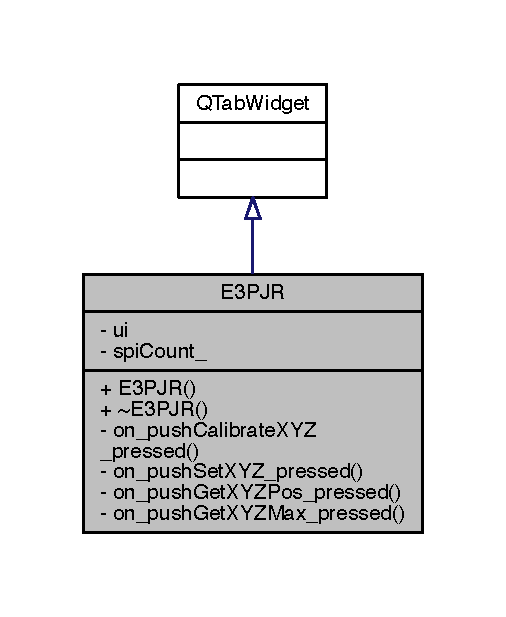
\includegraphics[width=243pt]{df/d11/class_e3_p_j_r__inherit__graph}
\end{center}
\end{figure}


Samarbejdsdiagram for E3\+P\+JR\+:\nopagebreak
\begin{figure}[H]
\begin{center}
\leavevmode
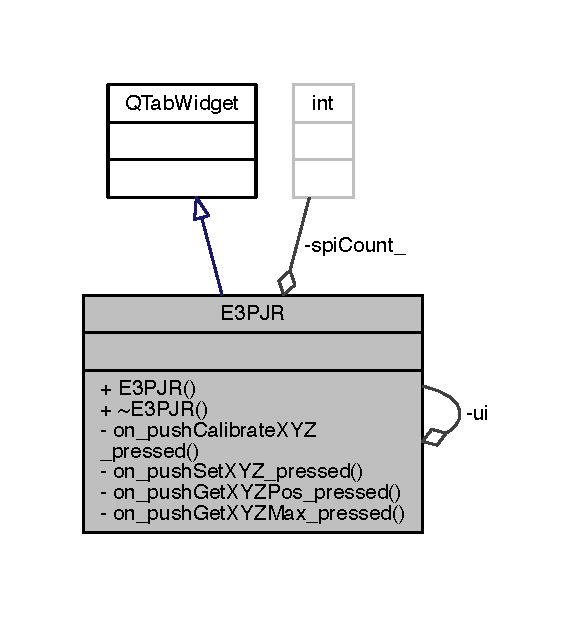
\includegraphics[width=275pt]{d5/d60/class_e3_p_j_r__coll__graph}
\end{center}
\end{figure}
\subsubsection*{Offentlige metoder}
\begin{DoxyCompactItemize}
\item 
\hyperlink{class_e3_p_j_r_a3a52bafbf77585b77f7cdfd3d5a2ab56}{E3\+P\+JR} (\hyperlink{class_q_widget}{Q\+Widget} $\ast$parent=0)
\item 
\hyperlink{class_e3_p_j_r_aeb532350a6ae56c292c37a6b983dffa2}{$\sim$\+E3\+P\+JR} ()
\end{DoxyCompactItemize}
\subsubsection*{Private slots}
\begin{DoxyCompactItemize}
\item 
void \hyperlink{class_e3_p_j_r_a6be58dfeec35962cafa418d47ebffc72}{on\+\_\+push\+Calibrate\+X\+Y\+Z\+\_\+pressed} ()
\item 
void \hyperlink{class_e3_p_j_r_af5298acfab7b21baee2e8eb8dd495ddb}{on\+\_\+push\+Set\+X\+Y\+Z\+\_\+pressed} ()
\item 
void \hyperlink{class_e3_p_j_r_a1384ab1d803de29103a58660ec602240}{on\+\_\+push\+Get\+X\+Y\+Z\+Pos\+\_\+pressed} ()
\item 
void \hyperlink{class_e3_p_j_r_a0230271a4b635131924f64f1fa354345}{on\+\_\+push\+Get\+X\+Y\+Z\+Max\+\_\+pressed} ()
\end{DoxyCompactItemize}
\subsubsection*{Private attributter}
\begin{DoxyCompactItemize}
\item 
\hyperlink{class_ui_1_1_e3_p_j_r}{Ui\+::\+E3\+P\+JR} $\ast$ \hyperlink{class_e3_p_j_r_a253979c6b115fd717a42bc24d84427c5}{ui}
\item 
int \hyperlink{class_e3_p_j_r_ab3c3e25d51904424592449e6dd0d813f}{spi\+Count\+\_\+}
\end{DoxyCompactItemize}


\subsubsection{Detaljeret beskrivelse}


Defineret på linje 15 i filen e3pjr.\+h.



\subsubsection{Dokumentation af konstruktører og destruktører}
\index{E3\+P\+JR@{E3\+P\+JR}!E3\+P\+JR@{E3\+P\+JR}}
\index{E3\+P\+JR@{E3\+P\+JR}!E3\+P\+JR@{E3\+P\+JR}}
\paragraph[{\texorpdfstring{E3\+P\+J\+R(\+Q\+Widget $\ast$parent=0)}{E3PJR(QWidget *parent=0)}}]{\setlength{\rightskip}{0pt plus 5cm}{\bf E3\+P\+JR} (
\begin{DoxyParamCaption}
\item[{{\bf Q\+Widget} $\ast$}]{parent = {\ttfamily 0}}
\end{DoxyParamCaption}
)\hspace{0.3cm}{\ttfamily [explicit]}}\hypertarget{class_e3_p_j_r_a3a52bafbf77585b77f7cdfd3d5a2ab56}{}\label{class_e3_p_j_r_a3a52bafbf77585b77f7cdfd3d5a2ab56}
\index{E3\+P\+JR@{E3\+P\+JR}!````~E3\+P\+JR@{$\sim$\+E3\+P\+JR}}
\index{````~E3\+P\+JR@{$\sim$\+E3\+P\+JR}!E3\+P\+JR@{E3\+P\+JR}}
\paragraph[{\texorpdfstring{$\sim$\+E3\+P\+J\+R()}{~E3PJR()}}]{\setlength{\rightskip}{0pt plus 5cm}$\sim${\bf E3\+P\+JR} (
\begin{DoxyParamCaption}
{}
\end{DoxyParamCaption}
)}\hypertarget{class_e3_p_j_r_aeb532350a6ae56c292c37a6b983dffa2}{}\label{class_e3_p_j_r_aeb532350a6ae56c292c37a6b983dffa2}


\subsubsection{Dokumentation af medlemsfunktioner}
\index{E3\+P\+JR@{E3\+P\+JR}!on\+\_\+push\+Calibrate\+X\+Y\+Z\+\_\+pressed@{on\+\_\+push\+Calibrate\+X\+Y\+Z\+\_\+pressed}}
\index{on\+\_\+push\+Calibrate\+X\+Y\+Z\+\_\+pressed@{on\+\_\+push\+Calibrate\+X\+Y\+Z\+\_\+pressed}!E3\+P\+JR@{E3\+P\+JR}}
\paragraph[{\texorpdfstring{on\+\_\+push\+Calibrate\+X\+Y\+Z\+\_\+pressed}{on_pushCalibrateXYZ_pressed}}]{\setlength{\rightskip}{0pt plus 5cm}void on\+\_\+push\+Calibrate\+X\+Y\+Z\+\_\+pressed (
\begin{DoxyParamCaption}
{}
\end{DoxyParamCaption}
)\hspace{0.3cm}{\ttfamily [private]}, {\ttfamily [slot]}}\hypertarget{class_e3_p_j_r_a6be58dfeec35962cafa418d47ebffc72}{}\label{class_e3_p_j_r_a6be58dfeec35962cafa418d47ebffc72}
\index{E3\+P\+JR@{E3\+P\+JR}!on\+\_\+push\+Get\+X\+Y\+Z\+Max\+\_\+pressed@{on\+\_\+push\+Get\+X\+Y\+Z\+Max\+\_\+pressed}}
\index{on\+\_\+push\+Get\+X\+Y\+Z\+Max\+\_\+pressed@{on\+\_\+push\+Get\+X\+Y\+Z\+Max\+\_\+pressed}!E3\+P\+JR@{E3\+P\+JR}}
\paragraph[{\texorpdfstring{on\+\_\+push\+Get\+X\+Y\+Z\+Max\+\_\+pressed}{on_pushGetXYZMax_pressed}}]{\setlength{\rightskip}{0pt plus 5cm}void on\+\_\+push\+Get\+X\+Y\+Z\+Max\+\_\+pressed (
\begin{DoxyParamCaption}
{}
\end{DoxyParamCaption}
)\hspace{0.3cm}{\ttfamily [private]}, {\ttfamily [slot]}}\hypertarget{class_e3_p_j_r_a0230271a4b635131924f64f1fa354345}{}\label{class_e3_p_j_r_a0230271a4b635131924f64f1fa354345}
\index{E3\+P\+JR@{E3\+P\+JR}!on\+\_\+push\+Get\+X\+Y\+Z\+Pos\+\_\+pressed@{on\+\_\+push\+Get\+X\+Y\+Z\+Pos\+\_\+pressed}}
\index{on\+\_\+push\+Get\+X\+Y\+Z\+Pos\+\_\+pressed@{on\+\_\+push\+Get\+X\+Y\+Z\+Pos\+\_\+pressed}!E3\+P\+JR@{E3\+P\+JR}}
\paragraph[{\texorpdfstring{on\+\_\+push\+Get\+X\+Y\+Z\+Pos\+\_\+pressed}{on_pushGetXYZPos_pressed}}]{\setlength{\rightskip}{0pt plus 5cm}void on\+\_\+push\+Get\+X\+Y\+Z\+Pos\+\_\+pressed (
\begin{DoxyParamCaption}
{}
\end{DoxyParamCaption}
)\hspace{0.3cm}{\ttfamily [private]}, {\ttfamily [slot]}}\hypertarget{class_e3_p_j_r_a1384ab1d803de29103a58660ec602240}{}\label{class_e3_p_j_r_a1384ab1d803de29103a58660ec602240}
\index{E3\+P\+JR@{E3\+P\+JR}!on\+\_\+push\+Set\+X\+Y\+Z\+\_\+pressed@{on\+\_\+push\+Set\+X\+Y\+Z\+\_\+pressed}}
\index{on\+\_\+push\+Set\+X\+Y\+Z\+\_\+pressed@{on\+\_\+push\+Set\+X\+Y\+Z\+\_\+pressed}!E3\+P\+JR@{E3\+P\+JR}}
\paragraph[{\texorpdfstring{on\+\_\+push\+Set\+X\+Y\+Z\+\_\+pressed}{on_pushSetXYZ_pressed}}]{\setlength{\rightskip}{0pt plus 5cm}void on\+\_\+push\+Set\+X\+Y\+Z\+\_\+pressed (
\begin{DoxyParamCaption}
{}
\end{DoxyParamCaption}
)\hspace{0.3cm}{\ttfamily [private]}, {\ttfamily [slot]}}\hypertarget{class_e3_p_j_r_af5298acfab7b21baee2e8eb8dd495ddb}{}\label{class_e3_p_j_r_af5298acfab7b21baee2e8eb8dd495ddb}


\subsubsection{Felt-\/dokumentation}
\index{E3\+P\+JR@{E3\+P\+JR}!spi\+Count\+\_\+@{spi\+Count\+\_\+}}
\index{spi\+Count\+\_\+@{spi\+Count\+\_\+}!E3\+P\+JR@{E3\+P\+JR}}
\paragraph[{\texorpdfstring{spi\+Count\+\_\+}{spiCount_}}]{\setlength{\rightskip}{0pt plus 5cm}int spi\+Count\+\_\+\hspace{0.3cm}{\ttfamily [private]}}\hypertarget{class_e3_p_j_r_ab3c3e25d51904424592449e6dd0d813f}{}\label{class_e3_p_j_r_ab3c3e25d51904424592449e6dd0d813f}


Defineret på linje 38 i filen e3pjr.\+h.

\index{E3\+P\+JR@{E3\+P\+JR}!ui@{ui}}
\index{ui@{ui}!E3\+P\+JR@{E3\+P\+JR}}
\paragraph[{\texorpdfstring{ui}{ui}}]{\setlength{\rightskip}{0pt plus 5cm}{\bf Ui\+::\+E3\+P\+JR}$\ast$ ui\hspace{0.3cm}{\ttfamily [private]}}\hypertarget{class_e3_p_j_r_a253979c6b115fd717a42bc24d84427c5}{}\label{class_e3_p_j_r_a253979c6b115fd717a42bc24d84427c5}


Defineret på linje 37 i filen e3pjr.\+h.



Dokumentationen for denne klasse blev genereret ud fra filen\+:\begin{DoxyCompactItemize}
\item 
\hyperlink{e3pjr_8h}{e3pjr.\+h}\end{DoxyCompactItemize}

\hypertarget{class_ui_1_1_e3_p_j_r}{}\subsection{E3\+P\+JR Klasse-\/reference}
\label{class_ui_1_1_e3_p_j_r}\index{E3\+P\+JR@{E3\+P\+JR}}


{\ttfamily \#include $<$ui\+\_\+e3pjr.\+h$>$}



Stamtræ for E3\+P\+JR\+:
\nopagebreak
\begin{figure}[H]
\begin{center}
\leavevmode
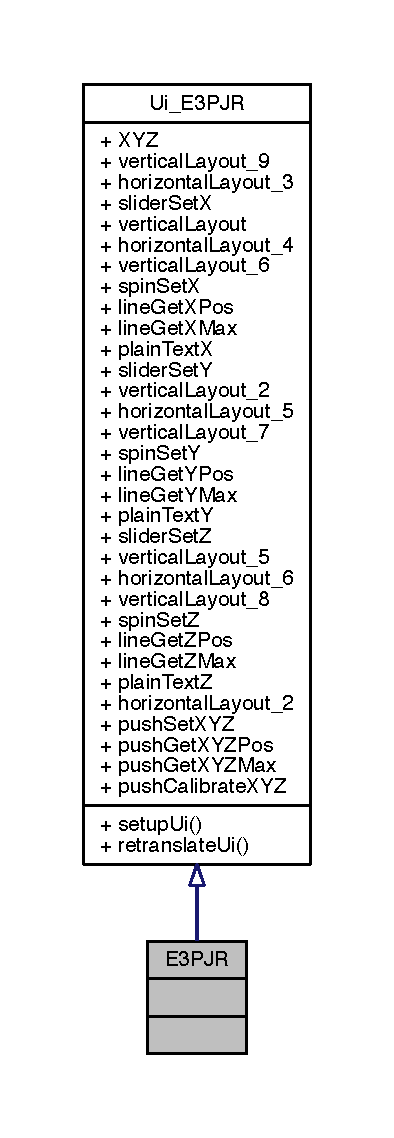
\includegraphics[width=189pt]{class_ui_1_1_e3_p_j_r__inherit__graph}
\end{center}
\end{figure}


Samarbejdsdiagram for E3\+P\+JR\+:
\nopagebreak
\begin{figure}[H]
\begin{center}
\leavevmode
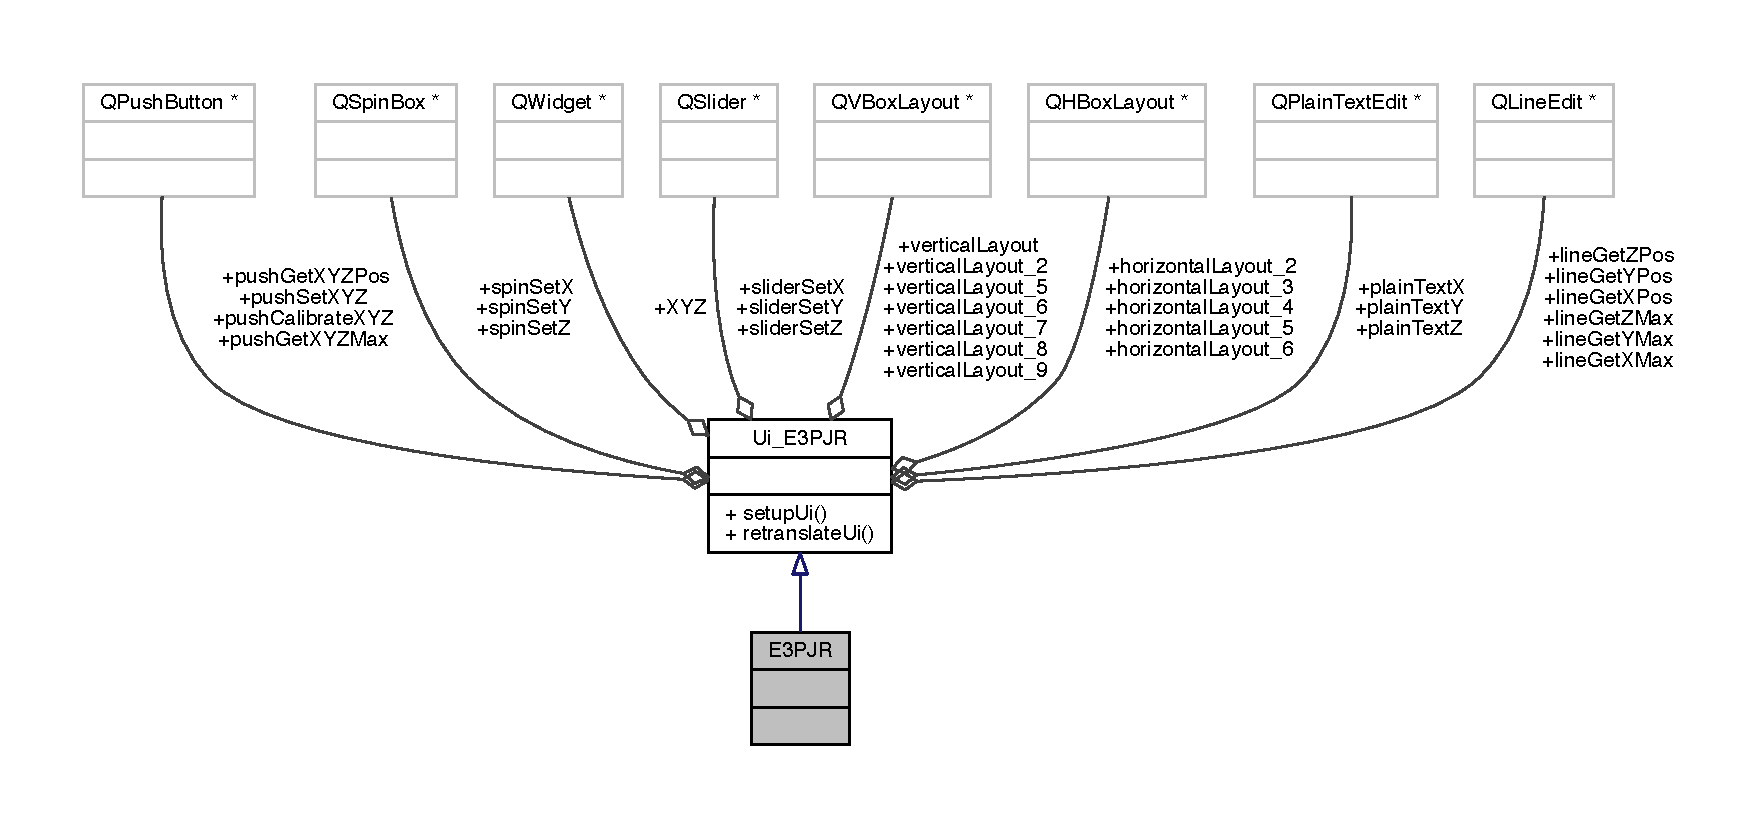
\includegraphics[width=350pt]{class_ui_1_1_e3_p_j_r__coll__graph}
\end{center}
\end{figure}
\subsubsection*{Offentlige metoder}
\begin{DoxyCompactItemize}
\item 
void \hyperlink{class_ui___e3_p_j_r_acd00a207b203ce4e08e2d4fe020281d2}{setup\+Ui} (\hyperlink{class_q_tab_widget}{Q\+Tab\+Widget} $\ast$\hyperlink{class_ui_1_1_e3_p_j_r}{E3\+P\+JR})
\item 
void \hyperlink{class_ui___e3_p_j_r_ab4d1867d3517a19d5b74c57ffd921202}{retranslate\+Ui} (\hyperlink{class_q_tab_widget}{Q\+Tab\+Widget} $\ast$\hyperlink{class_ui_1_1_e3_p_j_r}{E3\+P\+JR})
\end{DoxyCompactItemize}
\subsubsection*{Datafelter}
\begin{DoxyCompactItemize}
\item 
\hyperlink{class_q_widget}{Q\+Widget} $\ast$ \hyperlink{class_ui___e3_p_j_r_a098a80b873d9e0a09fd834f09e5028b4}{X\+YZ}
\item 
Q\+V\+Box\+Layout $\ast$ \hyperlink{class_ui___e3_p_j_r_a7c00a0b53a83fa0709131b996a6249a9}{vertical\+Layout\+\_\+9}
\item 
Q\+H\+Box\+Layout $\ast$ \hyperlink{class_ui___e3_p_j_r_af1b2167ad3027fe2c2328701164e54ec}{horizontal\+Layout\+\_\+3}
\item 
Q\+Slider $\ast$ \hyperlink{class_ui___e3_p_j_r_ac45c355780da0c571a472ccb5f74c977}{slider\+SetX}
\item 
Q\+V\+Box\+Layout $\ast$ \hyperlink{class_ui___e3_p_j_r_ad85f9339d941aa92fe82db7dcba6664c}{vertical\+Layout}
\item 
Q\+H\+Box\+Layout $\ast$ \hyperlink{class_ui___e3_p_j_r_aeb3eff1a8b0673c92f1ed957263d272b}{horizontal\+Layout\+\_\+4}
\item 
Q\+V\+Box\+Layout $\ast$ \hyperlink{class_ui___e3_p_j_r_a123f4222372065593b6a3433ac1dde9d}{vertical\+Layout\+\_\+6}
\item 
Q\+Spin\+Box $\ast$ \hyperlink{class_ui___e3_p_j_r_ab782845855d3c29e2d229ff09b717771}{spin\+SetX}
\item 
Q\+Line\+Edit $\ast$ \hyperlink{class_ui___e3_p_j_r_a2aa996a4bf178178f8c776bd139e1e98}{line\+Get\+X\+Pos}
\item 
Q\+Line\+Edit $\ast$ \hyperlink{class_ui___e3_p_j_r_aa70a702ff832048eb7b3a06560b1cccd}{line\+Get\+X\+Max}
\item 
Q\+Plain\+Text\+Edit $\ast$ \hyperlink{class_ui___e3_p_j_r_ac06b3dba512fbdc4436a33323fd6e737}{plain\+TextX}
\item 
Q\+Slider $\ast$ \hyperlink{class_ui___e3_p_j_r_afc14eb4b41f896c3881b1f3f86ebb5ab}{slider\+SetY}
\item 
Q\+V\+Box\+Layout $\ast$ \hyperlink{class_ui___e3_p_j_r_a1f81b7e95162efcbe551b64ca41869c8}{vertical\+Layout\+\_\+2}
\item 
Q\+H\+Box\+Layout $\ast$ \hyperlink{class_ui___e3_p_j_r_a9200504b29bbbfa17f9e6aefafc2c122}{horizontal\+Layout\+\_\+5}
\item 
Q\+V\+Box\+Layout $\ast$ \hyperlink{class_ui___e3_p_j_r_a6846ec6f18ab0ea13bdb2d00b2cb3947}{vertical\+Layout\+\_\+7}
\item 
Q\+Spin\+Box $\ast$ \hyperlink{class_ui___e3_p_j_r_a855f6972ba1dc6a61308080e1dea2447}{spin\+SetY}
\item 
Q\+Line\+Edit $\ast$ \hyperlink{class_ui___e3_p_j_r_af7a504d650e35e560d66d6e9cc2ec20e}{line\+Get\+Y\+Pos}
\item 
Q\+Line\+Edit $\ast$ \hyperlink{class_ui___e3_p_j_r_a6db76c359ac491d1e084a0febda62fa8}{line\+Get\+Y\+Max}
\item 
Q\+Plain\+Text\+Edit $\ast$ \hyperlink{class_ui___e3_p_j_r_aded895240a26d5b3349be548e863fcd2}{plain\+TextY}
\item 
Q\+Slider $\ast$ \hyperlink{class_ui___e3_p_j_r_a6ef8bc7a96e71c14d44d1573f43506d4}{slider\+SetZ}
\item 
Q\+V\+Box\+Layout $\ast$ \hyperlink{class_ui___e3_p_j_r_acbe0600e63ca9c63fe807730289e677a}{vertical\+Layout\+\_\+5}
\item 
Q\+H\+Box\+Layout $\ast$ \hyperlink{class_ui___e3_p_j_r_aee7bbbb4f14e80e5c3821623d9c4d52b}{horizontal\+Layout\+\_\+6}
\item 
Q\+V\+Box\+Layout $\ast$ \hyperlink{class_ui___e3_p_j_r_aecbd2cafbe12abcd4a5a7865aad8d917}{vertical\+Layout\+\_\+8}
\item 
Q\+Spin\+Box $\ast$ \hyperlink{class_ui___e3_p_j_r_a1c5f1bef8dc94bae1a91139a37d1d881}{spin\+SetZ}
\item 
Q\+Line\+Edit $\ast$ \hyperlink{class_ui___e3_p_j_r_af271cd40f5223cbdb1803e41493746cc}{line\+Get\+Z\+Pos}
\item 
Q\+Line\+Edit $\ast$ \hyperlink{class_ui___e3_p_j_r_a4bd5e082a2fb51522d5606ed355289d5}{line\+Get\+Z\+Max}
\item 
Q\+Plain\+Text\+Edit $\ast$ \hyperlink{class_ui___e3_p_j_r_aa688da4507156fb25ab31678d45842c9}{plain\+TextZ}
\item 
Q\+H\+Box\+Layout $\ast$ \hyperlink{class_ui___e3_p_j_r_a535a43287b7a5605cfc11580d146d3fb}{horizontal\+Layout\+\_\+2}
\item 
Q\+Push\+Button $\ast$ \hyperlink{class_ui___e3_p_j_r_a95989982eaebbf117db602b9c5642fc5}{push\+Set\+X\+YZ}
\item 
Q\+Push\+Button $\ast$ \hyperlink{class_ui___e3_p_j_r_a5a172ff2cdd7f0b1731e866267981cd4}{push\+Get\+X\+Y\+Z\+Pos}
\item 
Q\+Push\+Button $\ast$ \hyperlink{class_ui___e3_p_j_r_a16f1701307e43c614a3c0aed623577b7}{push\+Get\+X\+Y\+Z\+Max}
\item 
Q\+Push\+Button $\ast$ \hyperlink{class_ui___e3_p_j_r_a0a82bc71b94b2c607f872cbcf936811a}{push\+Calibrate\+X\+YZ}
\end{DoxyCompactItemize}


\subsubsection{Detaljeret beskrivelse}


Defineret på linje 300 i filen ui\+\_\+e3pjr.\+h.



\subsubsection{Dokumentation af medlemsfunktioner}
\index{Ui\+::\+E3\+P\+JR@{Ui\+::\+E3\+P\+JR}!retranslate\+Ui@{retranslate\+Ui}}
\index{retranslate\+Ui@{retranslate\+Ui}!Ui\+::\+E3\+P\+JR@{Ui\+::\+E3\+P\+JR}}
\paragraph[{\texorpdfstring{retranslate\+Ui(\+Q\+Tab\+Widget $\ast$\+E3\+P\+J\+R)}{retranslateUi(QTabWidget *E3PJR)}}]{\setlength{\rightskip}{0pt plus 5cm}void retranslate\+Ui (
\begin{DoxyParamCaption}
\item[{{\bf Q\+Tab\+Widget} $\ast$}]{E3\+P\+JR}
\end{DoxyParamCaption}
)\hspace{0.3cm}{\ttfamily [inline]}, {\ttfamily [inherited]}}\hypertarget{class_ui___e3_p_j_r_ab4d1867d3517a19d5b74c57ffd921202}{}\label{class_ui___e3_p_j_r_ab4d1867d3517a19d5b74c57ffd921202}


Defineret på linje 281 i filen ui\+\_\+e3pjr.\+h.



Refereret til af Ui\+\_\+\+E3\+P\+J\+R\+::setup\+Ui().


\begin{DoxyCode}
282     \{
283         E3PJR->setWindowTitle(QApplication::translate(\textcolor{stringliteral}{"E3PJR"}, \textcolor{stringliteral}{"TabWidget"}, 0, QApplication::UnicodeUTF8));
284         \hyperlink{class_ui___e3_p_j_r_a2aa996a4bf178178f8c776bd139e1e98}{lineGetXPos}->setPlaceholderText(QApplication::translate(\textcolor{stringliteral}{"E3PJR"}, \textcolor{stringliteral}{"xPos"}, 0, 
      QApplication::UnicodeUTF8));
285         \hyperlink{class_ui___e3_p_j_r_aa70a702ff832048eb7b3a06560b1cccd}{lineGetXMax}->setPlaceholderText(QApplication::translate(\textcolor{stringliteral}{"E3PJR"}, \textcolor{stringliteral}{"xMax"}, 0, 
      QApplication::UnicodeUTF8));
286         \hyperlink{class_ui___e3_p_j_r_af7a504d650e35e560d66d6e9cc2ec20e}{lineGetYPos}->setPlaceholderText(QApplication::translate(\textcolor{stringliteral}{"E3PJR"}, \textcolor{stringliteral}{"yPos"}, 0, 
      QApplication::UnicodeUTF8));
287         \hyperlink{class_ui___e3_p_j_r_a6db76c359ac491d1e084a0febda62fa8}{lineGetYMax}->setPlaceholderText(QApplication::translate(\textcolor{stringliteral}{"E3PJR"}, \textcolor{stringliteral}{"yMax"}, 0, 
      QApplication::UnicodeUTF8));
288         \hyperlink{class_ui___e3_p_j_r_af271cd40f5223cbdb1803e41493746cc}{lineGetZPos}->setPlaceholderText(QApplication::translate(\textcolor{stringliteral}{"E3PJR"}, \textcolor{stringliteral}{"zPos"}, 0, 
      QApplication::UnicodeUTF8));
289         \hyperlink{class_ui___e3_p_j_r_a4bd5e082a2fb51522d5606ed355289d5}{lineGetZMax}->setPlaceholderText(QApplication::translate(\textcolor{stringliteral}{"E3PJR"}, \textcolor{stringliteral}{"zMax"}, 0, 
      QApplication::UnicodeUTF8));
290         \hyperlink{class_ui___e3_p_j_r_a95989982eaebbf117db602b9c5642fc5}{pushSetXYZ}->setText(QApplication::translate(\textcolor{stringliteral}{"E3PJR"}, \textcolor{stringliteral}{"SetXYZPos"}, 0, 
      QApplication::UnicodeUTF8));
291         \hyperlink{class_ui___e3_p_j_r_a5a172ff2cdd7f0b1731e866267981cd4}{pushGetXYZPos}->setText(QApplication::translate(\textcolor{stringliteral}{"E3PJR"}, \textcolor{stringliteral}{"GetXYZPos"}, 0, 
      QApplication::UnicodeUTF8));
292         \hyperlink{class_ui___e3_p_j_r_a16f1701307e43c614a3c0aed623577b7}{pushGetXYZMax}->setText(QApplication::translate(\textcolor{stringliteral}{"E3PJR"}, \textcolor{stringliteral}{"GetXYZMax"}, 0, 
      QApplication::UnicodeUTF8));
293         \hyperlink{class_ui___e3_p_j_r_a0a82bc71b94b2c607f872cbcf936811a}{pushCalibrateXYZ}->setText(QApplication::translate(\textcolor{stringliteral}{"E3PJR"}, \textcolor{stringliteral}{"CalibrateXYZ"}, 0, 
      QApplication::UnicodeUTF8));
294         E3PJR->setTabText(E3PJR->indexOf(\hyperlink{class_ui___e3_p_j_r_a098a80b873d9e0a09fd834f09e5028b4}{XYZ}), QApplication::translate(\textcolor{stringliteral}{"E3PJR"}, \textcolor{stringliteral}{"XYZ"}, 0, 
      QApplication::UnicodeUTF8));
295     \} \textcolor{comment}{// retranslateUi}
\end{DoxyCode}


Her er kalder-\/grafen for denne funktion\+:
\nopagebreak
\begin{figure}[H]
\begin{center}
\leavevmode
\includegraphics[width=239pt]{class_ui___e3_p_j_r_ab4d1867d3517a19d5b74c57ffd921202_icgraph}
\end{center}
\end{figure}


\index{Ui\+::\+E3\+P\+JR@{Ui\+::\+E3\+P\+JR}!setup\+Ui@{setup\+Ui}}
\index{setup\+Ui@{setup\+Ui}!Ui\+::\+E3\+P\+JR@{Ui\+::\+E3\+P\+JR}}
\paragraph[{\texorpdfstring{setup\+Ui(\+Q\+Tab\+Widget $\ast$\+E3\+P\+J\+R)}{setupUi(QTabWidget *E3PJR)}}]{\setlength{\rightskip}{0pt plus 5cm}void setup\+Ui (
\begin{DoxyParamCaption}
\item[{{\bf Q\+Tab\+Widget} $\ast$}]{E3\+P\+JR}
\end{DoxyParamCaption}
)\hspace{0.3cm}{\ttfamily [inline]}, {\ttfamily [inherited]}}\hypertarget{class_ui___e3_p_j_r_acd00a207b203ce4e08e2d4fe020281d2}{}\label{class_ui___e3_p_j_r_acd00a207b203ce4e08e2d4fe020281d2}


Defineret på linje 65 i filen ui\+\_\+e3pjr.\+h.



Indeholder referencer til Ui\+\_\+\+E3\+P\+J\+R\+::retranslate\+Ui().


\begin{DoxyCode}
66     \{
67         \textcolor{keywordflow}{if} (E3PJR->objectName().isEmpty())
68             E3PJR->setObjectName(QString::fromUtf8(\textcolor{stringliteral}{"E3PJR"}));
69         E3PJR->resize(480, 278);
70         \hyperlink{class_ui___e3_p_j_r_a098a80b873d9e0a09fd834f09e5028b4}{XYZ} = \textcolor{keyword}{new} \hyperlink{class_q_widget}{QWidget}();
71         \hyperlink{class_ui___e3_p_j_r_a098a80b873d9e0a09fd834f09e5028b4}{XYZ}->setObjectName(QString::fromUtf8(\textcolor{stringliteral}{"XYZ"}));
72         \hyperlink{class_ui___e3_p_j_r_a7c00a0b53a83fa0709131b996a6249a9}{verticalLayout\_9} = \textcolor{keyword}{new} QVBoxLayout(\hyperlink{class_ui___e3_p_j_r_a098a80b873d9e0a09fd834f09e5028b4}{XYZ});
73         \hyperlink{class_ui___e3_p_j_r_a7c00a0b53a83fa0709131b996a6249a9}{verticalLayout\_9}->setObjectName(QString::fromUtf8(\textcolor{stringliteral}{"verticalLayout\_9"}));
74         \hyperlink{class_ui___e3_p_j_r_af1b2167ad3027fe2c2328701164e54ec}{horizontalLayout\_3} = \textcolor{keyword}{new} QHBoxLayout();
75         \hyperlink{class_ui___e3_p_j_r_af1b2167ad3027fe2c2328701164e54ec}{horizontalLayout\_3}->setObjectName(QString::fromUtf8(\textcolor{stringliteral}{"horizontalLayout\_3"}));
76         \hyperlink{class_ui___e3_p_j_r_ac45c355780da0c571a472ccb5f74c977}{sliderSetX} = \textcolor{keyword}{new} QSlider(\hyperlink{class_ui___e3_p_j_r_a098a80b873d9e0a09fd834f09e5028b4}{XYZ});
77         \hyperlink{class_ui___e3_p_j_r_ac45c355780da0c571a472ccb5f74c977}{sliderSetX}->setObjectName(QString::fromUtf8(\textcolor{stringliteral}{"sliderSetX"}));
78         \hyperlink{class_ui___e3_p_j_r_ac45c355780da0c571a472ccb5f74c977}{sliderSetX}->setMaximum(255);
79         \hyperlink{class_ui___e3_p_j_r_ac45c355780da0c571a472ccb5f74c977}{sliderSetX}->setSingleStep(5);
80         \hyperlink{class_ui___e3_p_j_r_ac45c355780da0c571a472ccb5f74c977}{sliderSetX}->setPageStep(15);
81         \hyperlink{class_ui___e3_p_j_r_ac45c355780da0c571a472ccb5f74c977}{sliderSetX}->setOrientation(Qt::Vertical);
82 
83         \hyperlink{class_ui___e3_p_j_r_af1b2167ad3027fe2c2328701164e54ec}{horizontalLayout\_3}->addWidget(\hyperlink{class_ui___e3_p_j_r_ac45c355780da0c571a472ccb5f74c977}{sliderSetX});
84 
85         \hyperlink{class_ui___e3_p_j_r_ad85f9339d941aa92fe82db7dcba6664c}{verticalLayout} = \textcolor{keyword}{new} QVBoxLayout();
86         \hyperlink{class_ui___e3_p_j_r_ad85f9339d941aa92fe82db7dcba6664c}{verticalLayout}->setObjectName(QString::fromUtf8(\textcolor{stringliteral}{"verticalLayout"}));
87         \hyperlink{class_ui___e3_p_j_r_aeb3eff1a8b0673c92f1ed957263d272b}{horizontalLayout\_4} = \textcolor{keyword}{new} QHBoxLayout();
88         \hyperlink{class_ui___e3_p_j_r_aeb3eff1a8b0673c92f1ed957263d272b}{horizontalLayout\_4}->setObjectName(QString::fromUtf8(\textcolor{stringliteral}{"horizontalLayout\_4"}));
89         \hyperlink{class_ui___e3_p_j_r_a123f4222372065593b6a3433ac1dde9d}{verticalLayout\_6} = \textcolor{keyword}{new} QVBoxLayout();
90         \hyperlink{class_ui___e3_p_j_r_a123f4222372065593b6a3433ac1dde9d}{verticalLayout\_6}->setObjectName(QString::fromUtf8(\textcolor{stringliteral}{"verticalLayout\_6"}));
91         \hyperlink{class_ui___e3_p_j_r_ab782845855d3c29e2d229ff09b717771}{spinSetX} = \textcolor{keyword}{new} QSpinBox(\hyperlink{class_ui___e3_p_j_r_a098a80b873d9e0a09fd834f09e5028b4}{XYZ});
92         \hyperlink{class_ui___e3_p_j_r_ab782845855d3c29e2d229ff09b717771}{spinSetX}->setObjectName(QString::fromUtf8(\textcolor{stringliteral}{"spinSetX"}));
93         \hyperlink{class_ui___e3_p_j_r_ab782845855d3c29e2d229ff09b717771}{spinSetX}->setAlignment(Qt::AlignCenter);
94         \hyperlink{class_ui___e3_p_j_r_ab782845855d3c29e2d229ff09b717771}{spinSetX}->setMaximum(255);
95         \hyperlink{class_ui___e3_p_j_r_ab782845855d3c29e2d229ff09b717771}{spinSetX}->setSingleStep(5);
96 
97         \hyperlink{class_ui___e3_p_j_r_a123f4222372065593b6a3433ac1dde9d}{verticalLayout\_6}->addWidget(\hyperlink{class_ui___e3_p_j_r_ab782845855d3c29e2d229ff09b717771}{spinSetX});
98 
99         \hyperlink{class_ui___e3_p_j_r_a2aa996a4bf178178f8c776bd139e1e98}{lineGetXPos} = \textcolor{keyword}{new} QLineEdit(\hyperlink{class_ui___e3_p_j_r_a098a80b873d9e0a09fd834f09e5028b4}{XYZ});
100         \hyperlink{class_ui___e3_p_j_r_a2aa996a4bf178178f8c776bd139e1e98}{lineGetXPos}->setObjectName(QString::fromUtf8(\textcolor{stringliteral}{"lineGetXPos"}));
101         \hyperlink{class_ui___e3_p_j_r_a2aa996a4bf178178f8c776bd139e1e98}{lineGetXPos}->setAlignment(Qt::AlignCenter);
102 
103         \hyperlink{class_ui___e3_p_j_r_a123f4222372065593b6a3433ac1dde9d}{verticalLayout\_6}->addWidget(\hyperlink{class_ui___e3_p_j_r_a2aa996a4bf178178f8c776bd139e1e98}{lineGetXPos});
104 
105         \hyperlink{class_ui___e3_p_j_r_aa70a702ff832048eb7b3a06560b1cccd}{lineGetXMax} = \textcolor{keyword}{new} QLineEdit(\hyperlink{class_ui___e3_p_j_r_a098a80b873d9e0a09fd834f09e5028b4}{XYZ});
106         \hyperlink{class_ui___e3_p_j_r_aa70a702ff832048eb7b3a06560b1cccd}{lineGetXMax}->setObjectName(QString::fromUtf8(\textcolor{stringliteral}{"lineGetXMax"}));
107         \hyperlink{class_ui___e3_p_j_r_aa70a702ff832048eb7b3a06560b1cccd}{lineGetXMax}->setAlignment(Qt::AlignCenter);
108 
109         \hyperlink{class_ui___e3_p_j_r_a123f4222372065593b6a3433ac1dde9d}{verticalLayout\_6}->addWidget(\hyperlink{class_ui___e3_p_j_r_aa70a702ff832048eb7b3a06560b1cccd}{lineGetXMax});
110 
111 
112         \hyperlink{class_ui___e3_p_j_r_aeb3eff1a8b0673c92f1ed957263d272b}{horizontalLayout\_4}->addLayout(\hyperlink{class_ui___e3_p_j_r_a123f4222372065593b6a3433ac1dde9d}{verticalLayout\_6});
113 
114 
115         \hyperlink{class_ui___e3_p_j_r_ad85f9339d941aa92fe82db7dcba6664c}{verticalLayout}->addLayout(\hyperlink{class_ui___e3_p_j_r_aeb3eff1a8b0673c92f1ed957263d272b}{horizontalLayout\_4});
116 
117         \hyperlink{class_ui___e3_p_j_r_ac06b3dba512fbdc4436a33323fd6e737}{plainTextX} = \textcolor{keyword}{new} QPlainTextEdit(\hyperlink{class_ui___e3_p_j_r_a098a80b873d9e0a09fd834f09e5028b4}{XYZ});
118         \hyperlink{class_ui___e3_p_j_r_ac06b3dba512fbdc4436a33323fd6e737}{plainTextX}->setObjectName(QString::fromUtf8(\textcolor{stringliteral}{"plainTextX"}));
119         \hyperlink{class_ui___e3_p_j_r_ac06b3dba512fbdc4436a33323fd6e737}{plainTextX}->setVerticalScrollBarPolicy(Qt::ScrollBarAlwaysOff);
120         \hyperlink{class_ui___e3_p_j_r_ac06b3dba512fbdc4436a33323fd6e737}{plainTextX}->setHorizontalScrollBarPolicy(Qt::ScrollBarAlwaysOff);
121         \hyperlink{class_ui___e3_p_j_r_ac06b3dba512fbdc4436a33323fd6e737}{plainTextX}->setUndoRedoEnabled(\textcolor{keyword}{false});
122         \hyperlink{class_ui___e3_p_j_r_ac06b3dba512fbdc4436a33323fd6e737}{plainTextX}->setReadOnly(\textcolor{keyword}{true});
123         \hyperlink{class_ui___e3_p_j_r_ac06b3dba512fbdc4436a33323fd6e737}{plainTextX}->setOverwriteMode(\textcolor{keyword}{false});
124 
125         \hyperlink{class_ui___e3_p_j_r_ad85f9339d941aa92fe82db7dcba6664c}{verticalLayout}->addWidget(\hyperlink{class_ui___e3_p_j_r_ac06b3dba512fbdc4436a33323fd6e737}{plainTextX});
126 
127 
128         \hyperlink{class_ui___e3_p_j_r_af1b2167ad3027fe2c2328701164e54ec}{horizontalLayout\_3}->addLayout(\hyperlink{class_ui___e3_p_j_r_ad85f9339d941aa92fe82db7dcba6664c}{verticalLayout});
129 
130         \hyperlink{class_ui___e3_p_j_r_afc14eb4b41f896c3881b1f3f86ebb5ab}{sliderSetY} = \textcolor{keyword}{new} QSlider(\hyperlink{class_ui___e3_p_j_r_a098a80b873d9e0a09fd834f09e5028b4}{XYZ});
131         \hyperlink{class_ui___e3_p_j_r_afc14eb4b41f896c3881b1f3f86ebb5ab}{sliderSetY}->setObjectName(QString::fromUtf8(\textcolor{stringliteral}{"sliderSetY"}));
132         \hyperlink{class_ui___e3_p_j_r_afc14eb4b41f896c3881b1f3f86ebb5ab}{sliderSetY}->setMaximum(255);
133         \hyperlink{class_ui___e3_p_j_r_afc14eb4b41f896c3881b1f3f86ebb5ab}{sliderSetY}->setSingleStep(5);
134         \hyperlink{class_ui___e3_p_j_r_afc14eb4b41f896c3881b1f3f86ebb5ab}{sliderSetY}->setPageStep(15);
135         \hyperlink{class_ui___e3_p_j_r_afc14eb4b41f896c3881b1f3f86ebb5ab}{sliderSetY}->setOrientation(Qt::Vertical);
136 
137         \hyperlink{class_ui___e3_p_j_r_af1b2167ad3027fe2c2328701164e54ec}{horizontalLayout\_3}->addWidget(\hyperlink{class_ui___e3_p_j_r_afc14eb4b41f896c3881b1f3f86ebb5ab}{sliderSetY});
138 
139         \hyperlink{class_ui___e3_p_j_r_a1f81b7e95162efcbe551b64ca41869c8}{verticalLayout\_2} = \textcolor{keyword}{new} QVBoxLayout();
140         \hyperlink{class_ui___e3_p_j_r_a1f81b7e95162efcbe551b64ca41869c8}{verticalLayout\_2}->setObjectName(QString::fromUtf8(\textcolor{stringliteral}{"verticalLayout\_2"}));
141         \hyperlink{class_ui___e3_p_j_r_a9200504b29bbbfa17f9e6aefafc2c122}{horizontalLayout\_5} = \textcolor{keyword}{new} QHBoxLayout();
142         \hyperlink{class_ui___e3_p_j_r_a9200504b29bbbfa17f9e6aefafc2c122}{horizontalLayout\_5}->setObjectName(QString::fromUtf8(\textcolor{stringliteral}{"horizontalLayout\_5"}));
143         \hyperlink{class_ui___e3_p_j_r_a6846ec6f18ab0ea13bdb2d00b2cb3947}{verticalLayout\_7} = \textcolor{keyword}{new} QVBoxLayout();
144         \hyperlink{class_ui___e3_p_j_r_a6846ec6f18ab0ea13bdb2d00b2cb3947}{verticalLayout\_7}->setObjectName(QString::fromUtf8(\textcolor{stringliteral}{"verticalLayout\_7"}));
145         \hyperlink{class_ui___e3_p_j_r_a855f6972ba1dc6a61308080e1dea2447}{spinSetY} = \textcolor{keyword}{new} QSpinBox(\hyperlink{class_ui___e3_p_j_r_a098a80b873d9e0a09fd834f09e5028b4}{XYZ});
146         \hyperlink{class_ui___e3_p_j_r_a855f6972ba1dc6a61308080e1dea2447}{spinSetY}->setObjectName(QString::fromUtf8(\textcolor{stringliteral}{"spinSetY"}));
147         \hyperlink{class_ui___e3_p_j_r_a855f6972ba1dc6a61308080e1dea2447}{spinSetY}->setAlignment(Qt::AlignCenter);
148         \hyperlink{class_ui___e3_p_j_r_a855f6972ba1dc6a61308080e1dea2447}{spinSetY}->setMaximum(255);
149         \hyperlink{class_ui___e3_p_j_r_a855f6972ba1dc6a61308080e1dea2447}{spinSetY}->setSingleStep(5);
150 
151         \hyperlink{class_ui___e3_p_j_r_a6846ec6f18ab0ea13bdb2d00b2cb3947}{verticalLayout\_7}->addWidget(\hyperlink{class_ui___e3_p_j_r_a855f6972ba1dc6a61308080e1dea2447}{spinSetY});
152 
153         \hyperlink{class_ui___e3_p_j_r_af7a504d650e35e560d66d6e9cc2ec20e}{lineGetYPos} = \textcolor{keyword}{new} QLineEdit(\hyperlink{class_ui___e3_p_j_r_a098a80b873d9e0a09fd834f09e5028b4}{XYZ});
154         \hyperlink{class_ui___e3_p_j_r_af7a504d650e35e560d66d6e9cc2ec20e}{lineGetYPos}->setObjectName(QString::fromUtf8(\textcolor{stringliteral}{"lineGetYPos"}));
155         \hyperlink{class_ui___e3_p_j_r_af7a504d650e35e560d66d6e9cc2ec20e}{lineGetYPos}->setAlignment(Qt::AlignCenter);
156 
157         \hyperlink{class_ui___e3_p_j_r_a6846ec6f18ab0ea13bdb2d00b2cb3947}{verticalLayout\_7}->addWidget(\hyperlink{class_ui___e3_p_j_r_af7a504d650e35e560d66d6e9cc2ec20e}{lineGetYPos});
158 
159         \hyperlink{class_ui___e3_p_j_r_a6db76c359ac491d1e084a0febda62fa8}{lineGetYMax} = \textcolor{keyword}{new} QLineEdit(\hyperlink{class_ui___e3_p_j_r_a098a80b873d9e0a09fd834f09e5028b4}{XYZ});
160         \hyperlink{class_ui___e3_p_j_r_a6db76c359ac491d1e084a0febda62fa8}{lineGetYMax}->setObjectName(QString::fromUtf8(\textcolor{stringliteral}{"lineGetYMax"}));
161         \hyperlink{class_ui___e3_p_j_r_a6db76c359ac491d1e084a0febda62fa8}{lineGetYMax}->setAlignment(Qt::AlignCenter);
162 
163         \hyperlink{class_ui___e3_p_j_r_a6846ec6f18ab0ea13bdb2d00b2cb3947}{verticalLayout\_7}->addWidget(\hyperlink{class_ui___e3_p_j_r_a6db76c359ac491d1e084a0febda62fa8}{lineGetYMax});
164 
165 
166         \hyperlink{class_ui___e3_p_j_r_a9200504b29bbbfa17f9e6aefafc2c122}{horizontalLayout\_5}->addLayout(\hyperlink{class_ui___e3_p_j_r_a6846ec6f18ab0ea13bdb2d00b2cb3947}{verticalLayout\_7});
167 
168 
169         \hyperlink{class_ui___e3_p_j_r_a1f81b7e95162efcbe551b64ca41869c8}{verticalLayout\_2}->addLayout(\hyperlink{class_ui___e3_p_j_r_a9200504b29bbbfa17f9e6aefafc2c122}{horizontalLayout\_5});
170 
171         \hyperlink{class_ui___e3_p_j_r_aded895240a26d5b3349be548e863fcd2}{plainTextY} = \textcolor{keyword}{new} QPlainTextEdit(\hyperlink{class_ui___e3_p_j_r_a098a80b873d9e0a09fd834f09e5028b4}{XYZ});
172         \hyperlink{class_ui___e3_p_j_r_aded895240a26d5b3349be548e863fcd2}{plainTextY}->setObjectName(QString::fromUtf8(\textcolor{stringliteral}{"plainTextY"}));
173         \hyperlink{class_ui___e3_p_j_r_aded895240a26d5b3349be548e863fcd2}{plainTextY}->setVerticalScrollBarPolicy(Qt::ScrollBarAlwaysOff);
174         \hyperlink{class_ui___e3_p_j_r_aded895240a26d5b3349be548e863fcd2}{plainTextY}->setHorizontalScrollBarPolicy(Qt::ScrollBarAlwaysOff);
175         \hyperlink{class_ui___e3_p_j_r_aded895240a26d5b3349be548e863fcd2}{plainTextY}->setUndoRedoEnabled(\textcolor{keyword}{false});
176         \hyperlink{class_ui___e3_p_j_r_aded895240a26d5b3349be548e863fcd2}{plainTextY}->setReadOnly(\textcolor{keyword}{true});
177 
178         \hyperlink{class_ui___e3_p_j_r_a1f81b7e95162efcbe551b64ca41869c8}{verticalLayout\_2}->addWidget(\hyperlink{class_ui___e3_p_j_r_aded895240a26d5b3349be548e863fcd2}{plainTextY});
179 
180 
181         \hyperlink{class_ui___e3_p_j_r_af1b2167ad3027fe2c2328701164e54ec}{horizontalLayout\_3}->addLayout(\hyperlink{class_ui___e3_p_j_r_a1f81b7e95162efcbe551b64ca41869c8}{verticalLayout\_2});
182 
183         \hyperlink{class_ui___e3_p_j_r_a6ef8bc7a96e71c14d44d1573f43506d4}{sliderSetZ} = \textcolor{keyword}{new} QSlider(\hyperlink{class_ui___e3_p_j_r_a098a80b873d9e0a09fd834f09e5028b4}{XYZ});
184         \hyperlink{class_ui___e3_p_j_r_a6ef8bc7a96e71c14d44d1573f43506d4}{sliderSetZ}->setObjectName(QString::fromUtf8(\textcolor{stringliteral}{"sliderSetZ"}));
185         \hyperlink{class_ui___e3_p_j_r_a6ef8bc7a96e71c14d44d1573f43506d4}{sliderSetZ}->setMaximum(255);
186         \hyperlink{class_ui___e3_p_j_r_a6ef8bc7a96e71c14d44d1573f43506d4}{sliderSetZ}->setSingleStep(5);
187         \hyperlink{class_ui___e3_p_j_r_a6ef8bc7a96e71c14d44d1573f43506d4}{sliderSetZ}->setPageStep(15);
188         \hyperlink{class_ui___e3_p_j_r_a6ef8bc7a96e71c14d44d1573f43506d4}{sliderSetZ}->setOrientation(Qt::Vertical);
189 
190         \hyperlink{class_ui___e3_p_j_r_af1b2167ad3027fe2c2328701164e54ec}{horizontalLayout\_3}->addWidget(\hyperlink{class_ui___e3_p_j_r_a6ef8bc7a96e71c14d44d1573f43506d4}{sliderSetZ});
191 
192         \hyperlink{class_ui___e3_p_j_r_acbe0600e63ca9c63fe807730289e677a}{verticalLayout\_5} = \textcolor{keyword}{new} QVBoxLayout();
193         \hyperlink{class_ui___e3_p_j_r_acbe0600e63ca9c63fe807730289e677a}{verticalLayout\_5}->setObjectName(QString::fromUtf8(\textcolor{stringliteral}{"verticalLayout\_5"}));
194         \hyperlink{class_ui___e3_p_j_r_aee7bbbb4f14e80e5c3821623d9c4d52b}{horizontalLayout\_6} = \textcolor{keyword}{new} QHBoxLayout();
195         \hyperlink{class_ui___e3_p_j_r_aee7bbbb4f14e80e5c3821623d9c4d52b}{horizontalLayout\_6}->setObjectName(QString::fromUtf8(\textcolor{stringliteral}{"horizontalLayout\_6"}));
196         \hyperlink{class_ui___e3_p_j_r_aecbd2cafbe12abcd4a5a7865aad8d917}{verticalLayout\_8} = \textcolor{keyword}{new} QVBoxLayout();
197         \hyperlink{class_ui___e3_p_j_r_aecbd2cafbe12abcd4a5a7865aad8d917}{verticalLayout\_8}->setObjectName(QString::fromUtf8(\textcolor{stringliteral}{"verticalLayout\_8"}));
198         \hyperlink{class_ui___e3_p_j_r_a1c5f1bef8dc94bae1a91139a37d1d881}{spinSetZ} = \textcolor{keyword}{new} QSpinBox(\hyperlink{class_ui___e3_p_j_r_a098a80b873d9e0a09fd834f09e5028b4}{XYZ});
199         \hyperlink{class_ui___e3_p_j_r_a1c5f1bef8dc94bae1a91139a37d1d881}{spinSetZ}->setObjectName(QString::fromUtf8(\textcolor{stringliteral}{"spinSetZ"}));
200         \hyperlink{class_ui___e3_p_j_r_a1c5f1bef8dc94bae1a91139a37d1d881}{spinSetZ}->setAlignment(Qt::AlignCenter);
201         \hyperlink{class_ui___e3_p_j_r_a1c5f1bef8dc94bae1a91139a37d1d881}{spinSetZ}->setMaximum(255);
202         \hyperlink{class_ui___e3_p_j_r_a1c5f1bef8dc94bae1a91139a37d1d881}{spinSetZ}->setSingleStep(5);
203 
204         \hyperlink{class_ui___e3_p_j_r_aecbd2cafbe12abcd4a5a7865aad8d917}{verticalLayout\_8}->addWidget(\hyperlink{class_ui___e3_p_j_r_a1c5f1bef8dc94bae1a91139a37d1d881}{spinSetZ});
205 
206         \hyperlink{class_ui___e3_p_j_r_af271cd40f5223cbdb1803e41493746cc}{lineGetZPos} = \textcolor{keyword}{new} QLineEdit(\hyperlink{class_ui___e3_p_j_r_a098a80b873d9e0a09fd834f09e5028b4}{XYZ});
207         \hyperlink{class_ui___e3_p_j_r_af271cd40f5223cbdb1803e41493746cc}{lineGetZPos}->setObjectName(QString::fromUtf8(\textcolor{stringliteral}{"lineGetZPos"}));
208         \hyperlink{class_ui___e3_p_j_r_af271cd40f5223cbdb1803e41493746cc}{lineGetZPos}->setAlignment(Qt::AlignCenter);
209 
210         \hyperlink{class_ui___e3_p_j_r_aecbd2cafbe12abcd4a5a7865aad8d917}{verticalLayout\_8}->addWidget(\hyperlink{class_ui___e3_p_j_r_af271cd40f5223cbdb1803e41493746cc}{lineGetZPos});
211 
212         \hyperlink{class_ui___e3_p_j_r_a4bd5e082a2fb51522d5606ed355289d5}{lineGetZMax} = \textcolor{keyword}{new} QLineEdit(\hyperlink{class_ui___e3_p_j_r_a098a80b873d9e0a09fd834f09e5028b4}{XYZ});
213         \hyperlink{class_ui___e3_p_j_r_a4bd5e082a2fb51522d5606ed355289d5}{lineGetZMax}->setObjectName(QString::fromUtf8(\textcolor{stringliteral}{"lineGetZMax"}));
214         \hyperlink{class_ui___e3_p_j_r_a4bd5e082a2fb51522d5606ed355289d5}{lineGetZMax}->setAlignment(Qt::AlignCenter);
215 
216         \hyperlink{class_ui___e3_p_j_r_aecbd2cafbe12abcd4a5a7865aad8d917}{verticalLayout\_8}->addWidget(\hyperlink{class_ui___e3_p_j_r_a4bd5e082a2fb51522d5606ed355289d5}{lineGetZMax});
217 
218 
219         \hyperlink{class_ui___e3_p_j_r_aee7bbbb4f14e80e5c3821623d9c4d52b}{horizontalLayout\_6}->addLayout(\hyperlink{class_ui___e3_p_j_r_aecbd2cafbe12abcd4a5a7865aad8d917}{verticalLayout\_8});
220 
221 
222         \hyperlink{class_ui___e3_p_j_r_acbe0600e63ca9c63fe807730289e677a}{verticalLayout\_5}->addLayout(\hyperlink{class_ui___e3_p_j_r_aee7bbbb4f14e80e5c3821623d9c4d52b}{horizontalLayout\_6});
223 
224         \hyperlink{class_ui___e3_p_j_r_aa688da4507156fb25ab31678d45842c9}{plainTextZ} = \textcolor{keyword}{new} QPlainTextEdit(\hyperlink{class_ui___e3_p_j_r_a098a80b873d9e0a09fd834f09e5028b4}{XYZ});
225         \hyperlink{class_ui___e3_p_j_r_aa688da4507156fb25ab31678d45842c9}{plainTextZ}->setObjectName(QString::fromUtf8(\textcolor{stringliteral}{"plainTextZ"}));
226         \hyperlink{class_ui___e3_p_j_r_aa688da4507156fb25ab31678d45842c9}{plainTextZ}->setVerticalScrollBarPolicy(Qt::ScrollBarAlwaysOff);
227         \hyperlink{class_ui___e3_p_j_r_aa688da4507156fb25ab31678d45842c9}{plainTextZ}->setHorizontalScrollBarPolicy(Qt::ScrollBarAlwaysOff);
228         \hyperlink{class_ui___e3_p_j_r_aa688da4507156fb25ab31678d45842c9}{plainTextZ}->setUndoRedoEnabled(\textcolor{keyword}{false});
229         \hyperlink{class_ui___e3_p_j_r_aa688da4507156fb25ab31678d45842c9}{plainTextZ}->setReadOnly(\textcolor{keyword}{true});
230 
231         \hyperlink{class_ui___e3_p_j_r_acbe0600e63ca9c63fe807730289e677a}{verticalLayout\_5}->addWidget(\hyperlink{class_ui___e3_p_j_r_aa688da4507156fb25ab31678d45842c9}{plainTextZ});
232 
233 
234         \hyperlink{class_ui___e3_p_j_r_af1b2167ad3027fe2c2328701164e54ec}{horizontalLayout\_3}->addLayout(\hyperlink{class_ui___e3_p_j_r_acbe0600e63ca9c63fe807730289e677a}{verticalLayout\_5});
235 
236 
237         \hyperlink{class_ui___e3_p_j_r_a7c00a0b53a83fa0709131b996a6249a9}{verticalLayout\_9}->addLayout(\hyperlink{class_ui___e3_p_j_r_af1b2167ad3027fe2c2328701164e54ec}{horizontalLayout\_3});
238 
239         \hyperlink{class_ui___e3_p_j_r_a535a43287b7a5605cfc11580d146d3fb}{horizontalLayout\_2} = \textcolor{keyword}{new} QHBoxLayout();
240         \hyperlink{class_ui___e3_p_j_r_a535a43287b7a5605cfc11580d146d3fb}{horizontalLayout\_2}->setObjectName(QString::fromUtf8(\textcolor{stringliteral}{"horizontalLayout\_2"}));
241         \hyperlink{class_ui___e3_p_j_r_a95989982eaebbf117db602b9c5642fc5}{pushSetXYZ} = \textcolor{keyword}{new} QPushButton(\hyperlink{class_ui___e3_p_j_r_a098a80b873d9e0a09fd834f09e5028b4}{XYZ});
242         \hyperlink{class_ui___e3_p_j_r_a95989982eaebbf117db602b9c5642fc5}{pushSetXYZ}->setObjectName(QString::fromUtf8(\textcolor{stringliteral}{"pushSetXYZ"}));
243 
244         \hyperlink{class_ui___e3_p_j_r_a535a43287b7a5605cfc11580d146d3fb}{horizontalLayout\_2}->addWidget(\hyperlink{class_ui___e3_p_j_r_a95989982eaebbf117db602b9c5642fc5}{pushSetXYZ});
245 
246         \hyperlink{class_ui___e3_p_j_r_a5a172ff2cdd7f0b1731e866267981cd4}{pushGetXYZPos} = \textcolor{keyword}{new} QPushButton(\hyperlink{class_ui___e3_p_j_r_a098a80b873d9e0a09fd834f09e5028b4}{XYZ});
247         \hyperlink{class_ui___e3_p_j_r_a5a172ff2cdd7f0b1731e866267981cd4}{pushGetXYZPos}->setObjectName(QString::fromUtf8(\textcolor{stringliteral}{"pushGetXYZPos"}));
248 
249         \hyperlink{class_ui___e3_p_j_r_a535a43287b7a5605cfc11580d146d3fb}{horizontalLayout\_2}->addWidget(\hyperlink{class_ui___e3_p_j_r_a5a172ff2cdd7f0b1731e866267981cd4}{pushGetXYZPos});
250 
251         \hyperlink{class_ui___e3_p_j_r_a16f1701307e43c614a3c0aed623577b7}{pushGetXYZMax} = \textcolor{keyword}{new} QPushButton(\hyperlink{class_ui___e3_p_j_r_a098a80b873d9e0a09fd834f09e5028b4}{XYZ});
252         \hyperlink{class_ui___e3_p_j_r_a16f1701307e43c614a3c0aed623577b7}{pushGetXYZMax}->setObjectName(QString::fromUtf8(\textcolor{stringliteral}{"pushGetXYZMax"}));
253 
254         \hyperlink{class_ui___e3_p_j_r_a535a43287b7a5605cfc11580d146d3fb}{horizontalLayout\_2}->addWidget(\hyperlink{class_ui___e3_p_j_r_a16f1701307e43c614a3c0aed623577b7}{pushGetXYZMax});
255 
256         \hyperlink{class_ui___e3_p_j_r_a0a82bc71b94b2c607f872cbcf936811a}{pushCalibrateXYZ} = \textcolor{keyword}{new} QPushButton(\hyperlink{class_ui___e3_p_j_r_a098a80b873d9e0a09fd834f09e5028b4}{XYZ});
257         \hyperlink{class_ui___e3_p_j_r_a0a82bc71b94b2c607f872cbcf936811a}{pushCalibrateXYZ}->setObjectName(QString::fromUtf8(\textcolor{stringliteral}{"pushCalibrateXYZ"}));
258 
259         \hyperlink{class_ui___e3_p_j_r_a535a43287b7a5605cfc11580d146d3fb}{horizontalLayout\_2}->addWidget(\hyperlink{class_ui___e3_p_j_r_a0a82bc71b94b2c607f872cbcf936811a}{pushCalibrateXYZ});
260 
261 
262         \hyperlink{class_ui___e3_p_j_r_a7c00a0b53a83fa0709131b996a6249a9}{verticalLayout\_9}->addLayout(\hyperlink{class_ui___e3_p_j_r_a535a43287b7a5605cfc11580d146d3fb}{horizontalLayout\_2});
263 
264         E3PJR->addTab(\hyperlink{class_ui___e3_p_j_r_a098a80b873d9e0a09fd834f09e5028b4}{XYZ}, QString());
265         QWidget::setTabOrder(\hyperlink{class_ui___e3_p_j_r_a855f6972ba1dc6a61308080e1dea2447}{spinSetY}, \hyperlink{class_ui___e3_p_j_r_a1c5f1bef8dc94bae1a91139a37d1d881}{spinSetZ});
266 
267         \hyperlink{class_ui___e3_p_j_r_ab4d1867d3517a19d5b74c57ffd921202}{retranslateUi}(E3PJR);
268         QObject::connect(\hyperlink{class_ui___e3_p_j_r_afc14eb4b41f896c3881b1f3f86ebb5ab}{sliderSetY}, SIGNAL(valueChanged(\textcolor{keywordtype}{int})), 
      \hyperlink{class_ui___e3_p_j_r_a855f6972ba1dc6a61308080e1dea2447}{spinSetY}, SLOT(setValue(\textcolor{keywordtype}{int})));
269         QObject::connect(\hyperlink{class_ui___e3_p_j_r_a855f6972ba1dc6a61308080e1dea2447}{spinSetY}, SIGNAL(valueChanged(\textcolor{keywordtype}{int})), \hyperlink{class_ui___e3_p_j_r_afc14eb4b41f896c3881b1f3f86ebb5ab}{sliderSetY}, SLOT(setValue(\textcolor{keywordtype}{
      int})));
270         QObject::connect(\hyperlink{class_ui___e3_p_j_r_a6ef8bc7a96e71c14d44d1573f43506d4}{sliderSetZ}, SIGNAL(valueChanged(\textcolor{keywordtype}{int})), 
      \hyperlink{class_ui___e3_p_j_r_a1c5f1bef8dc94bae1a91139a37d1d881}{spinSetZ}, SLOT(setValue(\textcolor{keywordtype}{int})));
271         QObject::connect(\hyperlink{class_ui___e3_p_j_r_a1c5f1bef8dc94bae1a91139a37d1d881}{spinSetZ}, SIGNAL(valueChanged(\textcolor{keywordtype}{int})), \hyperlink{class_ui___e3_p_j_r_a6ef8bc7a96e71c14d44d1573f43506d4}{sliderSetZ}, SLOT(setValue(\textcolor{keywordtype}{
      int})));
272         QObject::connect(\hyperlink{class_ui___e3_p_j_r_ac45c355780da0c571a472ccb5f74c977}{sliderSetX}, SIGNAL(valueChanged(\textcolor{keywordtype}{int})), 
      \hyperlink{class_ui___e3_p_j_r_ab782845855d3c29e2d229ff09b717771}{spinSetX}, SLOT(setValue(\textcolor{keywordtype}{int})));
273         QObject::connect(\hyperlink{class_ui___e3_p_j_r_ab782845855d3c29e2d229ff09b717771}{spinSetX}, SIGNAL(valueChanged(\textcolor{keywordtype}{int})), \hyperlink{class_ui___e3_p_j_r_ac45c355780da0c571a472ccb5f74c977}{sliderSetX}, SLOT(setValue(\textcolor{keywordtype}{
      int})));
274 
275         E3PJR->setCurrentIndex(0);
276 
277 
278         QMetaObject::connectSlotsByName(E3PJR);
279     \} \textcolor{comment}{// setupUi}
\end{DoxyCode}


Her er kald-\/grafen for denne funktion\+:
\nopagebreak
\begin{figure}[H]
\begin{center}
\leavevmode
\includegraphics[width=239pt]{class_ui___e3_p_j_r_acd00a207b203ce4e08e2d4fe020281d2_cgraph}
\end{center}
\end{figure}




\subsubsection{Felt-\/dokumentation}
\index{Ui\+::\+E3\+P\+JR@{Ui\+::\+E3\+P\+JR}!horizontal\+Layout\+\_\+2@{horizontal\+Layout\+\_\+2}}
\index{horizontal\+Layout\+\_\+2@{horizontal\+Layout\+\_\+2}!Ui\+::\+E3\+P\+JR@{Ui\+::\+E3\+P\+JR}}
\paragraph[{\texorpdfstring{horizontal\+Layout\+\_\+2}{horizontalLayout_2}}]{\setlength{\rightskip}{0pt plus 5cm}Q\+H\+Box\+Layout$\ast$ horizontal\+Layout\+\_\+2\hspace{0.3cm}{\ttfamily [inherited]}}\hypertarget{class_ui___e3_p_j_r_a535a43287b7a5605cfc11580d146d3fb}{}\label{class_ui___e3_p_j_r_a535a43287b7a5605cfc11580d146d3fb}


Defineret på linje 59 i filen ui\+\_\+e3pjr.\+h.

\index{Ui\+::\+E3\+P\+JR@{Ui\+::\+E3\+P\+JR}!horizontal\+Layout\+\_\+3@{horizontal\+Layout\+\_\+3}}
\index{horizontal\+Layout\+\_\+3@{horizontal\+Layout\+\_\+3}!Ui\+::\+E3\+P\+JR@{Ui\+::\+E3\+P\+JR}}
\paragraph[{\texorpdfstring{horizontal\+Layout\+\_\+3}{horizontalLayout_3}}]{\setlength{\rightskip}{0pt plus 5cm}Q\+H\+Box\+Layout$\ast$ horizontal\+Layout\+\_\+3\hspace{0.3cm}{\ttfamily [inherited]}}\hypertarget{class_ui___e3_p_j_r_af1b2167ad3027fe2c2328701164e54ec}{}\label{class_ui___e3_p_j_r_af1b2167ad3027fe2c2328701164e54ec}


Defineret på linje 34 i filen ui\+\_\+e3pjr.\+h.

\index{Ui\+::\+E3\+P\+JR@{Ui\+::\+E3\+P\+JR}!horizontal\+Layout\+\_\+4@{horizontal\+Layout\+\_\+4}}
\index{horizontal\+Layout\+\_\+4@{horizontal\+Layout\+\_\+4}!Ui\+::\+E3\+P\+JR@{Ui\+::\+E3\+P\+JR}}
\paragraph[{\texorpdfstring{horizontal\+Layout\+\_\+4}{horizontalLayout_4}}]{\setlength{\rightskip}{0pt plus 5cm}Q\+H\+Box\+Layout$\ast$ horizontal\+Layout\+\_\+4\hspace{0.3cm}{\ttfamily [inherited]}}\hypertarget{class_ui___e3_p_j_r_aeb3eff1a8b0673c92f1ed957263d272b}{}\label{class_ui___e3_p_j_r_aeb3eff1a8b0673c92f1ed957263d272b}


Defineret på linje 37 i filen ui\+\_\+e3pjr.\+h.

\index{Ui\+::\+E3\+P\+JR@{Ui\+::\+E3\+P\+JR}!horizontal\+Layout\+\_\+5@{horizontal\+Layout\+\_\+5}}
\index{horizontal\+Layout\+\_\+5@{horizontal\+Layout\+\_\+5}!Ui\+::\+E3\+P\+JR@{Ui\+::\+E3\+P\+JR}}
\paragraph[{\texorpdfstring{horizontal\+Layout\+\_\+5}{horizontalLayout_5}}]{\setlength{\rightskip}{0pt plus 5cm}Q\+H\+Box\+Layout$\ast$ horizontal\+Layout\+\_\+5\hspace{0.3cm}{\ttfamily [inherited]}}\hypertarget{class_ui___e3_p_j_r_a9200504b29bbbfa17f9e6aefafc2c122}{}\label{class_ui___e3_p_j_r_a9200504b29bbbfa17f9e6aefafc2c122}


Defineret på linje 45 i filen ui\+\_\+e3pjr.\+h.

\index{Ui\+::\+E3\+P\+JR@{Ui\+::\+E3\+P\+JR}!horizontal\+Layout\+\_\+6@{horizontal\+Layout\+\_\+6}}
\index{horizontal\+Layout\+\_\+6@{horizontal\+Layout\+\_\+6}!Ui\+::\+E3\+P\+JR@{Ui\+::\+E3\+P\+JR}}
\paragraph[{\texorpdfstring{horizontal\+Layout\+\_\+6}{horizontalLayout_6}}]{\setlength{\rightskip}{0pt plus 5cm}Q\+H\+Box\+Layout$\ast$ horizontal\+Layout\+\_\+6\hspace{0.3cm}{\ttfamily [inherited]}}\hypertarget{class_ui___e3_p_j_r_aee7bbbb4f14e80e5c3821623d9c4d52b}{}\label{class_ui___e3_p_j_r_aee7bbbb4f14e80e5c3821623d9c4d52b}


Defineret på linje 53 i filen ui\+\_\+e3pjr.\+h.

\index{Ui\+::\+E3\+P\+JR@{Ui\+::\+E3\+P\+JR}!line\+Get\+X\+Max@{line\+Get\+X\+Max}}
\index{line\+Get\+X\+Max@{line\+Get\+X\+Max}!Ui\+::\+E3\+P\+JR@{Ui\+::\+E3\+P\+JR}}
\paragraph[{\texorpdfstring{line\+Get\+X\+Max}{lineGetXMax}}]{\setlength{\rightskip}{0pt plus 5cm}Q\+Line\+Edit$\ast$ line\+Get\+X\+Max\hspace{0.3cm}{\ttfamily [inherited]}}\hypertarget{class_ui___e3_p_j_r_aa70a702ff832048eb7b3a06560b1cccd}{}\label{class_ui___e3_p_j_r_aa70a702ff832048eb7b3a06560b1cccd}


Defineret på linje 41 i filen ui\+\_\+e3pjr.\+h.

\index{Ui\+::\+E3\+P\+JR@{Ui\+::\+E3\+P\+JR}!line\+Get\+X\+Pos@{line\+Get\+X\+Pos}}
\index{line\+Get\+X\+Pos@{line\+Get\+X\+Pos}!Ui\+::\+E3\+P\+JR@{Ui\+::\+E3\+P\+JR}}
\paragraph[{\texorpdfstring{line\+Get\+X\+Pos}{lineGetXPos}}]{\setlength{\rightskip}{0pt plus 5cm}Q\+Line\+Edit$\ast$ line\+Get\+X\+Pos\hspace{0.3cm}{\ttfamily [inherited]}}\hypertarget{class_ui___e3_p_j_r_a2aa996a4bf178178f8c776bd139e1e98}{}\label{class_ui___e3_p_j_r_a2aa996a4bf178178f8c776bd139e1e98}


Defineret på linje 40 i filen ui\+\_\+e3pjr.\+h.

\index{Ui\+::\+E3\+P\+JR@{Ui\+::\+E3\+P\+JR}!line\+Get\+Y\+Max@{line\+Get\+Y\+Max}}
\index{line\+Get\+Y\+Max@{line\+Get\+Y\+Max}!Ui\+::\+E3\+P\+JR@{Ui\+::\+E3\+P\+JR}}
\paragraph[{\texorpdfstring{line\+Get\+Y\+Max}{lineGetYMax}}]{\setlength{\rightskip}{0pt plus 5cm}Q\+Line\+Edit$\ast$ line\+Get\+Y\+Max\hspace{0.3cm}{\ttfamily [inherited]}}\hypertarget{class_ui___e3_p_j_r_a6db76c359ac491d1e084a0febda62fa8}{}\label{class_ui___e3_p_j_r_a6db76c359ac491d1e084a0febda62fa8}


Defineret på linje 49 i filen ui\+\_\+e3pjr.\+h.

\index{Ui\+::\+E3\+P\+JR@{Ui\+::\+E3\+P\+JR}!line\+Get\+Y\+Pos@{line\+Get\+Y\+Pos}}
\index{line\+Get\+Y\+Pos@{line\+Get\+Y\+Pos}!Ui\+::\+E3\+P\+JR@{Ui\+::\+E3\+P\+JR}}
\paragraph[{\texorpdfstring{line\+Get\+Y\+Pos}{lineGetYPos}}]{\setlength{\rightskip}{0pt plus 5cm}Q\+Line\+Edit$\ast$ line\+Get\+Y\+Pos\hspace{0.3cm}{\ttfamily [inherited]}}\hypertarget{class_ui___e3_p_j_r_af7a504d650e35e560d66d6e9cc2ec20e}{}\label{class_ui___e3_p_j_r_af7a504d650e35e560d66d6e9cc2ec20e}


Defineret på linje 48 i filen ui\+\_\+e3pjr.\+h.

\index{Ui\+::\+E3\+P\+JR@{Ui\+::\+E3\+P\+JR}!line\+Get\+Z\+Max@{line\+Get\+Z\+Max}}
\index{line\+Get\+Z\+Max@{line\+Get\+Z\+Max}!Ui\+::\+E3\+P\+JR@{Ui\+::\+E3\+P\+JR}}
\paragraph[{\texorpdfstring{line\+Get\+Z\+Max}{lineGetZMax}}]{\setlength{\rightskip}{0pt plus 5cm}Q\+Line\+Edit$\ast$ line\+Get\+Z\+Max\hspace{0.3cm}{\ttfamily [inherited]}}\hypertarget{class_ui___e3_p_j_r_a4bd5e082a2fb51522d5606ed355289d5}{}\label{class_ui___e3_p_j_r_a4bd5e082a2fb51522d5606ed355289d5}


Defineret på linje 57 i filen ui\+\_\+e3pjr.\+h.

\index{Ui\+::\+E3\+P\+JR@{Ui\+::\+E3\+P\+JR}!line\+Get\+Z\+Pos@{line\+Get\+Z\+Pos}}
\index{line\+Get\+Z\+Pos@{line\+Get\+Z\+Pos}!Ui\+::\+E3\+P\+JR@{Ui\+::\+E3\+P\+JR}}
\paragraph[{\texorpdfstring{line\+Get\+Z\+Pos}{lineGetZPos}}]{\setlength{\rightskip}{0pt plus 5cm}Q\+Line\+Edit$\ast$ line\+Get\+Z\+Pos\hspace{0.3cm}{\ttfamily [inherited]}}\hypertarget{class_ui___e3_p_j_r_af271cd40f5223cbdb1803e41493746cc}{}\label{class_ui___e3_p_j_r_af271cd40f5223cbdb1803e41493746cc}


Defineret på linje 56 i filen ui\+\_\+e3pjr.\+h.

\index{Ui\+::\+E3\+P\+JR@{Ui\+::\+E3\+P\+JR}!plain\+TextX@{plain\+TextX}}
\index{plain\+TextX@{plain\+TextX}!Ui\+::\+E3\+P\+JR@{Ui\+::\+E3\+P\+JR}}
\paragraph[{\texorpdfstring{plain\+TextX}{plainTextX}}]{\setlength{\rightskip}{0pt plus 5cm}Q\+Plain\+Text\+Edit$\ast$ plain\+TextX\hspace{0.3cm}{\ttfamily [inherited]}}\hypertarget{class_ui___e3_p_j_r_ac06b3dba512fbdc4436a33323fd6e737}{}\label{class_ui___e3_p_j_r_ac06b3dba512fbdc4436a33323fd6e737}


Defineret på linje 42 i filen ui\+\_\+e3pjr.\+h.

\index{Ui\+::\+E3\+P\+JR@{Ui\+::\+E3\+P\+JR}!plain\+TextY@{plain\+TextY}}
\index{plain\+TextY@{plain\+TextY}!Ui\+::\+E3\+P\+JR@{Ui\+::\+E3\+P\+JR}}
\paragraph[{\texorpdfstring{plain\+TextY}{plainTextY}}]{\setlength{\rightskip}{0pt plus 5cm}Q\+Plain\+Text\+Edit$\ast$ plain\+TextY\hspace{0.3cm}{\ttfamily [inherited]}}\hypertarget{class_ui___e3_p_j_r_aded895240a26d5b3349be548e863fcd2}{}\label{class_ui___e3_p_j_r_aded895240a26d5b3349be548e863fcd2}


Defineret på linje 50 i filen ui\+\_\+e3pjr.\+h.

\index{Ui\+::\+E3\+P\+JR@{Ui\+::\+E3\+P\+JR}!plain\+TextZ@{plain\+TextZ}}
\index{plain\+TextZ@{plain\+TextZ}!Ui\+::\+E3\+P\+JR@{Ui\+::\+E3\+P\+JR}}
\paragraph[{\texorpdfstring{plain\+TextZ}{plainTextZ}}]{\setlength{\rightskip}{0pt plus 5cm}Q\+Plain\+Text\+Edit$\ast$ plain\+TextZ\hspace{0.3cm}{\ttfamily [inherited]}}\hypertarget{class_ui___e3_p_j_r_aa688da4507156fb25ab31678d45842c9}{}\label{class_ui___e3_p_j_r_aa688da4507156fb25ab31678d45842c9}


Defineret på linje 58 i filen ui\+\_\+e3pjr.\+h.

\index{Ui\+::\+E3\+P\+JR@{Ui\+::\+E3\+P\+JR}!push\+Calibrate\+X\+YZ@{push\+Calibrate\+X\+YZ}}
\index{push\+Calibrate\+X\+YZ@{push\+Calibrate\+X\+YZ}!Ui\+::\+E3\+P\+JR@{Ui\+::\+E3\+P\+JR}}
\paragraph[{\texorpdfstring{push\+Calibrate\+X\+YZ}{pushCalibrateXYZ}}]{\setlength{\rightskip}{0pt plus 5cm}Q\+Push\+Button$\ast$ push\+Calibrate\+X\+YZ\hspace{0.3cm}{\ttfamily [inherited]}}\hypertarget{class_ui___e3_p_j_r_a0a82bc71b94b2c607f872cbcf936811a}{}\label{class_ui___e3_p_j_r_a0a82bc71b94b2c607f872cbcf936811a}


Defineret på linje 63 i filen ui\+\_\+e3pjr.\+h.

\index{Ui\+::\+E3\+P\+JR@{Ui\+::\+E3\+P\+JR}!push\+Get\+X\+Y\+Z\+Max@{push\+Get\+X\+Y\+Z\+Max}}
\index{push\+Get\+X\+Y\+Z\+Max@{push\+Get\+X\+Y\+Z\+Max}!Ui\+::\+E3\+P\+JR@{Ui\+::\+E3\+P\+JR}}
\paragraph[{\texorpdfstring{push\+Get\+X\+Y\+Z\+Max}{pushGetXYZMax}}]{\setlength{\rightskip}{0pt plus 5cm}Q\+Push\+Button$\ast$ push\+Get\+X\+Y\+Z\+Max\hspace{0.3cm}{\ttfamily [inherited]}}\hypertarget{class_ui___e3_p_j_r_a16f1701307e43c614a3c0aed623577b7}{}\label{class_ui___e3_p_j_r_a16f1701307e43c614a3c0aed623577b7}


Defineret på linje 62 i filen ui\+\_\+e3pjr.\+h.

\index{Ui\+::\+E3\+P\+JR@{Ui\+::\+E3\+P\+JR}!push\+Get\+X\+Y\+Z\+Pos@{push\+Get\+X\+Y\+Z\+Pos}}
\index{push\+Get\+X\+Y\+Z\+Pos@{push\+Get\+X\+Y\+Z\+Pos}!Ui\+::\+E3\+P\+JR@{Ui\+::\+E3\+P\+JR}}
\paragraph[{\texorpdfstring{push\+Get\+X\+Y\+Z\+Pos}{pushGetXYZPos}}]{\setlength{\rightskip}{0pt plus 5cm}Q\+Push\+Button$\ast$ push\+Get\+X\+Y\+Z\+Pos\hspace{0.3cm}{\ttfamily [inherited]}}\hypertarget{class_ui___e3_p_j_r_a5a172ff2cdd7f0b1731e866267981cd4}{}\label{class_ui___e3_p_j_r_a5a172ff2cdd7f0b1731e866267981cd4}


Defineret på linje 61 i filen ui\+\_\+e3pjr.\+h.

\index{Ui\+::\+E3\+P\+JR@{Ui\+::\+E3\+P\+JR}!push\+Set\+X\+YZ@{push\+Set\+X\+YZ}}
\index{push\+Set\+X\+YZ@{push\+Set\+X\+YZ}!Ui\+::\+E3\+P\+JR@{Ui\+::\+E3\+P\+JR}}
\paragraph[{\texorpdfstring{push\+Set\+X\+YZ}{pushSetXYZ}}]{\setlength{\rightskip}{0pt plus 5cm}Q\+Push\+Button$\ast$ push\+Set\+X\+YZ\hspace{0.3cm}{\ttfamily [inherited]}}\hypertarget{class_ui___e3_p_j_r_a95989982eaebbf117db602b9c5642fc5}{}\label{class_ui___e3_p_j_r_a95989982eaebbf117db602b9c5642fc5}


Defineret på linje 60 i filen ui\+\_\+e3pjr.\+h.

\index{Ui\+::\+E3\+P\+JR@{Ui\+::\+E3\+P\+JR}!slider\+SetX@{slider\+SetX}}
\index{slider\+SetX@{slider\+SetX}!Ui\+::\+E3\+P\+JR@{Ui\+::\+E3\+P\+JR}}
\paragraph[{\texorpdfstring{slider\+SetX}{sliderSetX}}]{\setlength{\rightskip}{0pt plus 5cm}Q\+Slider$\ast$ slider\+SetX\hspace{0.3cm}{\ttfamily [inherited]}}\hypertarget{class_ui___e3_p_j_r_ac45c355780da0c571a472ccb5f74c977}{}\label{class_ui___e3_p_j_r_ac45c355780da0c571a472ccb5f74c977}


Defineret på linje 35 i filen ui\+\_\+e3pjr.\+h.

\index{Ui\+::\+E3\+P\+JR@{Ui\+::\+E3\+P\+JR}!slider\+SetY@{slider\+SetY}}
\index{slider\+SetY@{slider\+SetY}!Ui\+::\+E3\+P\+JR@{Ui\+::\+E3\+P\+JR}}
\paragraph[{\texorpdfstring{slider\+SetY}{sliderSetY}}]{\setlength{\rightskip}{0pt plus 5cm}Q\+Slider$\ast$ slider\+SetY\hspace{0.3cm}{\ttfamily [inherited]}}\hypertarget{class_ui___e3_p_j_r_afc14eb4b41f896c3881b1f3f86ebb5ab}{}\label{class_ui___e3_p_j_r_afc14eb4b41f896c3881b1f3f86ebb5ab}


Defineret på linje 43 i filen ui\+\_\+e3pjr.\+h.

\index{Ui\+::\+E3\+P\+JR@{Ui\+::\+E3\+P\+JR}!slider\+SetZ@{slider\+SetZ}}
\index{slider\+SetZ@{slider\+SetZ}!Ui\+::\+E3\+P\+JR@{Ui\+::\+E3\+P\+JR}}
\paragraph[{\texorpdfstring{slider\+SetZ}{sliderSetZ}}]{\setlength{\rightskip}{0pt plus 5cm}Q\+Slider$\ast$ slider\+SetZ\hspace{0.3cm}{\ttfamily [inherited]}}\hypertarget{class_ui___e3_p_j_r_a6ef8bc7a96e71c14d44d1573f43506d4}{}\label{class_ui___e3_p_j_r_a6ef8bc7a96e71c14d44d1573f43506d4}


Defineret på linje 51 i filen ui\+\_\+e3pjr.\+h.

\index{Ui\+::\+E3\+P\+JR@{Ui\+::\+E3\+P\+JR}!spin\+SetX@{spin\+SetX}}
\index{spin\+SetX@{spin\+SetX}!Ui\+::\+E3\+P\+JR@{Ui\+::\+E3\+P\+JR}}
\paragraph[{\texorpdfstring{spin\+SetX}{spinSetX}}]{\setlength{\rightskip}{0pt plus 5cm}Q\+Spin\+Box$\ast$ spin\+SetX\hspace{0.3cm}{\ttfamily [inherited]}}\hypertarget{class_ui___e3_p_j_r_ab782845855d3c29e2d229ff09b717771}{}\label{class_ui___e3_p_j_r_ab782845855d3c29e2d229ff09b717771}


Defineret på linje 39 i filen ui\+\_\+e3pjr.\+h.

\index{Ui\+::\+E3\+P\+JR@{Ui\+::\+E3\+P\+JR}!spin\+SetY@{spin\+SetY}}
\index{spin\+SetY@{spin\+SetY}!Ui\+::\+E3\+P\+JR@{Ui\+::\+E3\+P\+JR}}
\paragraph[{\texorpdfstring{spin\+SetY}{spinSetY}}]{\setlength{\rightskip}{0pt plus 5cm}Q\+Spin\+Box$\ast$ spin\+SetY\hspace{0.3cm}{\ttfamily [inherited]}}\hypertarget{class_ui___e3_p_j_r_a855f6972ba1dc6a61308080e1dea2447}{}\label{class_ui___e3_p_j_r_a855f6972ba1dc6a61308080e1dea2447}


Defineret på linje 47 i filen ui\+\_\+e3pjr.\+h.

\index{Ui\+::\+E3\+P\+JR@{Ui\+::\+E3\+P\+JR}!spin\+SetZ@{spin\+SetZ}}
\index{spin\+SetZ@{spin\+SetZ}!Ui\+::\+E3\+P\+JR@{Ui\+::\+E3\+P\+JR}}
\paragraph[{\texorpdfstring{spin\+SetZ}{spinSetZ}}]{\setlength{\rightskip}{0pt plus 5cm}Q\+Spin\+Box$\ast$ spin\+SetZ\hspace{0.3cm}{\ttfamily [inherited]}}\hypertarget{class_ui___e3_p_j_r_a1c5f1bef8dc94bae1a91139a37d1d881}{}\label{class_ui___e3_p_j_r_a1c5f1bef8dc94bae1a91139a37d1d881}


Defineret på linje 55 i filen ui\+\_\+e3pjr.\+h.

\index{Ui\+::\+E3\+P\+JR@{Ui\+::\+E3\+P\+JR}!vertical\+Layout@{vertical\+Layout}}
\index{vertical\+Layout@{vertical\+Layout}!Ui\+::\+E3\+P\+JR@{Ui\+::\+E3\+P\+JR}}
\paragraph[{\texorpdfstring{vertical\+Layout}{verticalLayout}}]{\setlength{\rightskip}{0pt plus 5cm}Q\+V\+Box\+Layout$\ast$ vertical\+Layout\hspace{0.3cm}{\ttfamily [inherited]}}\hypertarget{class_ui___e3_p_j_r_ad85f9339d941aa92fe82db7dcba6664c}{}\label{class_ui___e3_p_j_r_ad85f9339d941aa92fe82db7dcba6664c}


Defineret på linje 36 i filen ui\+\_\+e3pjr.\+h.

\index{Ui\+::\+E3\+P\+JR@{Ui\+::\+E3\+P\+JR}!vertical\+Layout\+\_\+2@{vertical\+Layout\+\_\+2}}
\index{vertical\+Layout\+\_\+2@{vertical\+Layout\+\_\+2}!Ui\+::\+E3\+P\+JR@{Ui\+::\+E3\+P\+JR}}
\paragraph[{\texorpdfstring{vertical\+Layout\+\_\+2}{verticalLayout_2}}]{\setlength{\rightskip}{0pt plus 5cm}Q\+V\+Box\+Layout$\ast$ vertical\+Layout\+\_\+2\hspace{0.3cm}{\ttfamily [inherited]}}\hypertarget{class_ui___e3_p_j_r_a1f81b7e95162efcbe551b64ca41869c8}{}\label{class_ui___e3_p_j_r_a1f81b7e95162efcbe551b64ca41869c8}


Defineret på linje 44 i filen ui\+\_\+e3pjr.\+h.

\index{Ui\+::\+E3\+P\+JR@{Ui\+::\+E3\+P\+JR}!vertical\+Layout\+\_\+5@{vertical\+Layout\+\_\+5}}
\index{vertical\+Layout\+\_\+5@{vertical\+Layout\+\_\+5}!Ui\+::\+E3\+P\+JR@{Ui\+::\+E3\+P\+JR}}
\paragraph[{\texorpdfstring{vertical\+Layout\+\_\+5}{verticalLayout_5}}]{\setlength{\rightskip}{0pt plus 5cm}Q\+V\+Box\+Layout$\ast$ vertical\+Layout\+\_\+5\hspace{0.3cm}{\ttfamily [inherited]}}\hypertarget{class_ui___e3_p_j_r_acbe0600e63ca9c63fe807730289e677a}{}\label{class_ui___e3_p_j_r_acbe0600e63ca9c63fe807730289e677a}


Defineret på linje 52 i filen ui\+\_\+e3pjr.\+h.

\index{Ui\+::\+E3\+P\+JR@{Ui\+::\+E3\+P\+JR}!vertical\+Layout\+\_\+6@{vertical\+Layout\+\_\+6}}
\index{vertical\+Layout\+\_\+6@{vertical\+Layout\+\_\+6}!Ui\+::\+E3\+P\+JR@{Ui\+::\+E3\+P\+JR}}
\paragraph[{\texorpdfstring{vertical\+Layout\+\_\+6}{verticalLayout_6}}]{\setlength{\rightskip}{0pt plus 5cm}Q\+V\+Box\+Layout$\ast$ vertical\+Layout\+\_\+6\hspace{0.3cm}{\ttfamily [inherited]}}\hypertarget{class_ui___e3_p_j_r_a123f4222372065593b6a3433ac1dde9d}{}\label{class_ui___e3_p_j_r_a123f4222372065593b6a3433ac1dde9d}


Defineret på linje 38 i filen ui\+\_\+e3pjr.\+h.

\index{Ui\+::\+E3\+P\+JR@{Ui\+::\+E3\+P\+JR}!vertical\+Layout\+\_\+7@{vertical\+Layout\+\_\+7}}
\index{vertical\+Layout\+\_\+7@{vertical\+Layout\+\_\+7}!Ui\+::\+E3\+P\+JR@{Ui\+::\+E3\+P\+JR}}
\paragraph[{\texorpdfstring{vertical\+Layout\+\_\+7}{verticalLayout_7}}]{\setlength{\rightskip}{0pt plus 5cm}Q\+V\+Box\+Layout$\ast$ vertical\+Layout\+\_\+7\hspace{0.3cm}{\ttfamily [inherited]}}\hypertarget{class_ui___e3_p_j_r_a6846ec6f18ab0ea13bdb2d00b2cb3947}{}\label{class_ui___e3_p_j_r_a6846ec6f18ab0ea13bdb2d00b2cb3947}


Defineret på linje 46 i filen ui\+\_\+e3pjr.\+h.

\index{Ui\+::\+E3\+P\+JR@{Ui\+::\+E3\+P\+JR}!vertical\+Layout\+\_\+8@{vertical\+Layout\+\_\+8}}
\index{vertical\+Layout\+\_\+8@{vertical\+Layout\+\_\+8}!Ui\+::\+E3\+P\+JR@{Ui\+::\+E3\+P\+JR}}
\paragraph[{\texorpdfstring{vertical\+Layout\+\_\+8}{verticalLayout_8}}]{\setlength{\rightskip}{0pt plus 5cm}Q\+V\+Box\+Layout$\ast$ vertical\+Layout\+\_\+8\hspace{0.3cm}{\ttfamily [inherited]}}\hypertarget{class_ui___e3_p_j_r_aecbd2cafbe12abcd4a5a7865aad8d917}{}\label{class_ui___e3_p_j_r_aecbd2cafbe12abcd4a5a7865aad8d917}


Defineret på linje 54 i filen ui\+\_\+e3pjr.\+h.

\index{Ui\+::\+E3\+P\+JR@{Ui\+::\+E3\+P\+JR}!vertical\+Layout\+\_\+9@{vertical\+Layout\+\_\+9}}
\index{vertical\+Layout\+\_\+9@{vertical\+Layout\+\_\+9}!Ui\+::\+E3\+P\+JR@{Ui\+::\+E3\+P\+JR}}
\paragraph[{\texorpdfstring{vertical\+Layout\+\_\+9}{verticalLayout_9}}]{\setlength{\rightskip}{0pt plus 5cm}Q\+V\+Box\+Layout$\ast$ vertical\+Layout\+\_\+9\hspace{0.3cm}{\ttfamily [inherited]}}\hypertarget{class_ui___e3_p_j_r_a7c00a0b53a83fa0709131b996a6249a9}{}\label{class_ui___e3_p_j_r_a7c00a0b53a83fa0709131b996a6249a9}


Defineret på linje 33 i filen ui\+\_\+e3pjr.\+h.

\index{Ui\+::\+E3\+P\+JR@{Ui\+::\+E3\+P\+JR}!X\+YZ@{X\+YZ}}
\index{X\+YZ@{X\+YZ}!Ui\+::\+E3\+P\+JR@{Ui\+::\+E3\+P\+JR}}
\paragraph[{\texorpdfstring{X\+YZ}{XYZ}}]{\setlength{\rightskip}{0pt plus 5cm}{\bf Q\+Widget}$\ast$ X\+YZ\hspace{0.3cm}{\ttfamily [inherited]}}\hypertarget{class_ui___e3_p_j_r_a098a80b873d9e0a09fd834f09e5028b4}{}\label{class_ui___e3_p_j_r_a098a80b873d9e0a09fd834f09e5028b4}


Defineret på linje 32 i filen ui\+\_\+e3pjr.\+h.



Dokumentationen for denne klasse blev genereret ud fra filen\+:\begin{DoxyCompactItemize}
\item 
\hyperlink{ui__e3pjr_8h}{ui\+\_\+e3pjr.\+h}\end{DoxyCompactItemize}

\hypertarget{class_light}{}\subsection{Light Klasse-\/reference}
\label{class_light}\index{Light@{Light}}


{\ttfamily \#include $<$light.\+h$>$}



Stamtræ for Light\+:\nopagebreak
\begin{figure}[H]
\begin{center}
\leavevmode
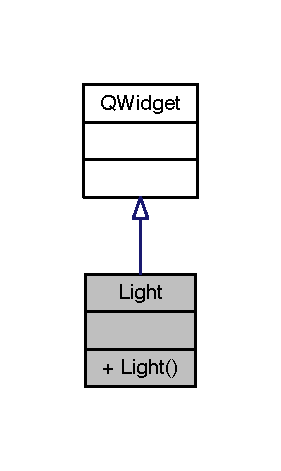
\includegraphics[width=135pt]{dd/d00/class_light__inherit__graph}
\end{center}
\end{figure}


Samarbejdsdiagram for Light\+:\nopagebreak
\begin{figure}[H]
\begin{center}
\leavevmode
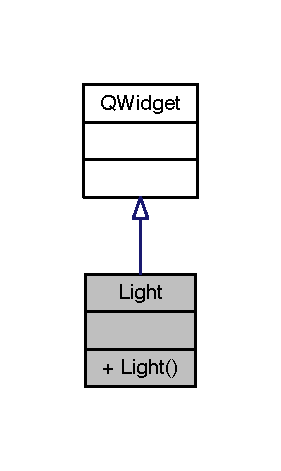
\includegraphics[width=135pt]{df/d88/class_light__coll__graph}
\end{center}
\end{figure}
\subsubsection*{Offentlige metoder}
\begin{DoxyCompactItemize}
\item 
\hyperlink{class_light_a6641ce3bc098be223d8e451bb3f5863d}{Light} (\hyperlink{class_q_widget}{Q\+Widget} $\ast$parent=0)
\end{DoxyCompactItemize}


\subsubsection{Detaljeret beskrivelse}


Defineret på linje 7 i filen light.\+h.



\subsubsection{Dokumentation af konstruktører og destruktører}
\index{Light@{Light}!Light@{Light}}
\index{Light@{Light}!Light@{Light}}
\paragraph[{\texorpdfstring{Light(\+Q\+Widget $\ast$parent=0)}{Light(QWidget *parent=0)}}]{\setlength{\rightskip}{0pt plus 5cm}{\bf Light} (
\begin{DoxyParamCaption}
\item[{{\bf Q\+Widget} $\ast$}]{parent = {\ttfamily 0}}
\end{DoxyParamCaption}
)\hspace{0.3cm}{\ttfamily [explicit]}}\hypertarget{class_light_a6641ce3bc098be223d8e451bb3f5863d}{}\label{class_light_a6641ce3bc098be223d8e451bb3f5863d}


Dokumentationen for denne klasse blev genereret ud fra filen\+:\begin{DoxyCompactItemize}
\item 
\hyperlink{light_8h}{light.\+h}\end{DoxyCompactItemize}

\hypertarget{class_main_display}{}\subsection{Main\+Display Klasse-\/reference}
\label{class_main_display}\index{Main\+Display@{Main\+Display}}


{\ttfamily \#include $<$maindisplay.\+h$>$}



Stamtræ for Main\+Display\+:\nopagebreak
\begin{figure}[H]
\begin{center}
\leavevmode
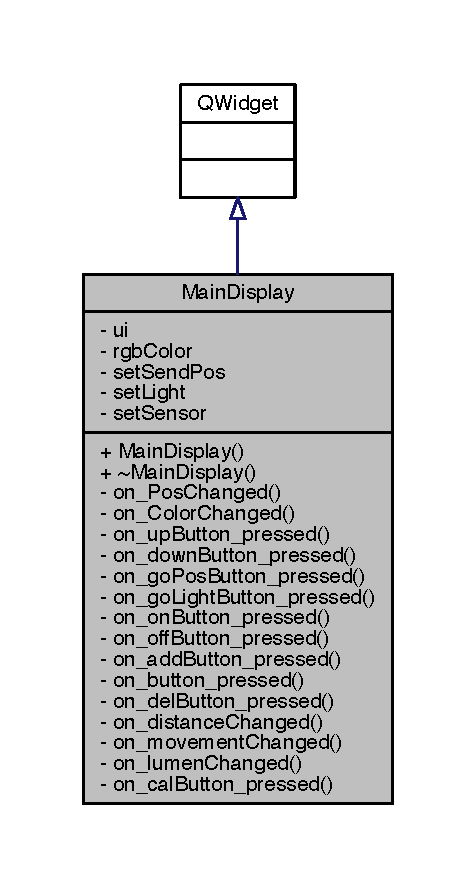
\includegraphics[width=228pt]{de/d64/class_main_display__inherit__graph}
\end{center}
\end{figure}


Samarbejdsdiagram for Main\+Display\+:\nopagebreak
\begin{figure}[H]
\begin{center}
\leavevmode
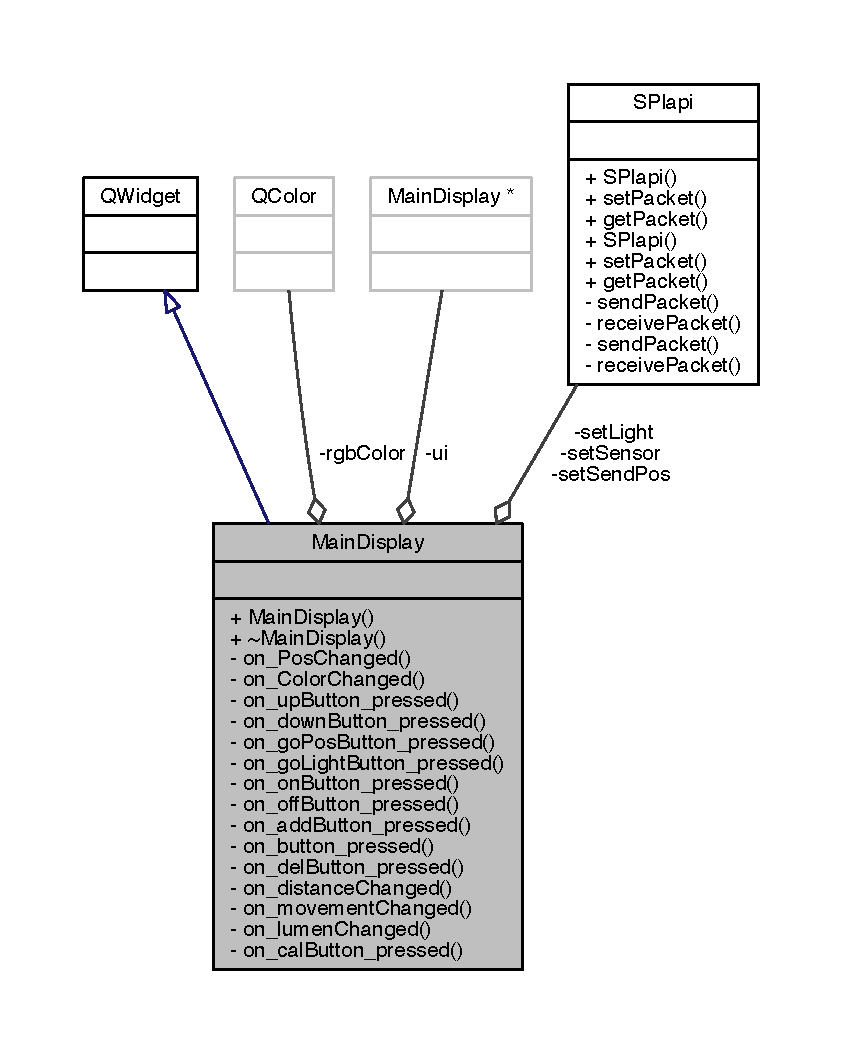
\includegraphics[width=350pt]{d2/d96/class_main_display__coll__graph}
\end{center}
\end{figure}
\subsubsection*{Offentlige metoder}
\begin{DoxyCompactItemize}
\item 
\hyperlink{class_main_display_a1b926c0907b4f58bf39a7192278aa28f}{Main\+Display} (\hyperlink{class_q_widget}{Q\+Widget} $\ast$parent=0)
\item 
\hyperlink{class_main_display_acc33b95d402516e0045bdff383c85d61}{$\sim$\+Main\+Display} ()
\end{DoxyCompactItemize}
\subsubsection*{Private slots}
\begin{DoxyCompactItemize}
\item 
void \hyperlink{class_main_display_a123b3d77e3bee2ee148d8e018c8fc35f}{on\+\_\+\+Pos\+Changed} ()
\item 
void \hyperlink{class_main_display_a52b87d1c28a3d284b47c2173fcc35f8e}{on\+\_\+\+Color\+Changed} ()
\item 
void \hyperlink{class_main_display_a9320639a3326230a7d8db24fa7171da4}{on\+\_\+up\+Button\+\_\+pressed} ()
\item 
void \hyperlink{class_main_display_a6c538b96e5bedc28eb06c557811b90be}{on\+\_\+down\+Button\+\_\+pressed} ()
\item 
void \hyperlink{class_main_display_a27f2ff12f69b04285d591a1933ee833e}{on\+\_\+go\+Pos\+Button\+\_\+pressed} ()
\item 
void \hyperlink{class_main_display_a627343d5a2d3faaaf356cc392ff3724c}{on\+\_\+go\+Light\+Button\+\_\+pressed} ()
\item 
void \hyperlink{class_main_display_aa72936be857d483be39f483e47067b75}{on\+\_\+on\+Button\+\_\+pressed} ()
\item 
void \hyperlink{class_main_display_a95c8436a234c95a8c990fe7823d8ebb6}{on\+\_\+off\+Button\+\_\+pressed} ()
\item 
void \hyperlink{class_main_display_acae8720b3bcb65341b5ae4d86e9ffa20}{on\+\_\+add\+Button\+\_\+pressed} ()
\item 
void \hyperlink{class_main_display_a69141f747223994d2d255f1fe23b58f6}{on\+\_\+button\+\_\+pressed} ()
\item 
void \hyperlink{class_main_display_a0f2757a17bb77793f0bb4cef1e619965}{on\+\_\+del\+Button\+\_\+pressed} ()
\item 
void \hyperlink{class_main_display_a4b959c3cf5ded11e93a21114ff00aba0}{on\+\_\+distance\+Changed} ()
\item 
void \hyperlink{class_main_display_a1682973e67a6796e43212fd9a7c5b62b}{on\+\_\+movement\+Changed} ()
\item 
void \hyperlink{class_main_display_a103eb76611e18718537d519bfe5df028}{on\+\_\+lumen\+Changed} ()
\item 
void \hyperlink{class_main_display_a6b0c30743c4c4db509af1d7a19da5f0f}{on\+\_\+cal\+Button\+\_\+pressed} ()
\end{DoxyCompactItemize}
\subsubsection*{Private attributter}
\begin{DoxyCompactItemize}
\item 
Ui\+::\+Main\+Display $\ast$ \hyperlink{class_main_display_ade778ccd9663d675377dae469e67b043}{ui}
\item 
Q\+Color \hyperlink{class_main_display_a2f85bb87f3dc79a58e445e310baf22ba}{rgb\+Color}
\item 
\hyperlink{class_s_p_iapi}{S\+P\+Iapi} \hyperlink{class_main_display_a7ff46364fccea06e07f178ebe035db21}{set\+Send\+Pos}
\item 
\hyperlink{class_s_p_iapi}{S\+P\+Iapi} \hyperlink{class_main_display_a807635feb3bf9a05bbcdb3682731726f}{set\+Light}
\item 
\hyperlink{class_s_p_iapi}{S\+P\+Iapi} \hyperlink{class_main_display_a320f575ecd3ce1e9b630703d8146b748}{set\+Sensor}
\end{DoxyCompactItemize}


\subsubsection{Detaljeret beskrivelse}
\begin{DoxyAuthor}{Forfatter}
Victor Busk (\href{mailto:201409557@post.au.dk}{\tt 201409557@post.\+au.\+dk}) 
\end{DoxyAuthor}


Defineret på linje 19 i filen maindisplay.\+h.



\subsubsection{Dokumentation af konstruktører og destruktører}
\index{Main\+Display@{Main\+Display}!Main\+Display@{Main\+Display}}
\index{Main\+Display@{Main\+Display}!Main\+Display@{Main\+Display}}
\paragraph[{\texorpdfstring{Main\+Display(\+Q\+Widget $\ast$parent=0)}{MainDisplay(QWidget *parent=0)}}]{\setlength{\rightskip}{0pt plus 5cm}{\bf Main\+Display} (
\begin{DoxyParamCaption}
\item[{{\bf Q\+Widget} $\ast$}]{parent = {\ttfamily 0}}
\end{DoxyParamCaption}
)\hspace{0.3cm}{\ttfamily [explicit]}}\hypertarget{class_main_display_a1b926c0907b4f58bf39a7192278aa28f}{}\label{class_main_display_a1b926c0907b4f58bf39a7192278aa28f}
\index{Main\+Display@{Main\+Display}!````~Main\+Display@{$\sim$\+Main\+Display}}
\index{````~Main\+Display@{$\sim$\+Main\+Display}!Main\+Display@{Main\+Display}}
\paragraph[{\texorpdfstring{$\sim$\+Main\+Display()}{~MainDisplay()}}]{\setlength{\rightskip}{0pt plus 5cm}$\sim${\bf Main\+Display} (
\begin{DoxyParamCaption}
{}
\end{DoxyParamCaption}
)}\hypertarget{class_main_display_acc33b95d402516e0045bdff383c85d61}{}\label{class_main_display_acc33b95d402516e0045bdff383c85d61}


\subsubsection{Dokumentation af medlemsfunktioner}
\index{Main\+Display@{Main\+Display}!on\+\_\+add\+Button\+\_\+pressed@{on\+\_\+add\+Button\+\_\+pressed}}
\index{on\+\_\+add\+Button\+\_\+pressed@{on\+\_\+add\+Button\+\_\+pressed}!Main\+Display@{Main\+Display}}
\paragraph[{\texorpdfstring{on\+\_\+add\+Button\+\_\+pressed}{on_addButton_pressed}}]{\setlength{\rightskip}{0pt plus 5cm}void on\+\_\+add\+Button\+\_\+pressed (
\begin{DoxyParamCaption}
{}
\end{DoxyParamCaption}
)\hspace{0.3cm}{\ttfamily [private]}, {\ttfamily [slot]}}\hypertarget{class_main_display_acae8720b3bcb65341b5ae4d86e9ffa20}{}\label{class_main_display_acae8720b3bcb65341b5ae4d86e9ffa20}
\index{Main\+Display@{Main\+Display}!on\+\_\+button\+\_\+pressed@{on\+\_\+button\+\_\+pressed}}
\index{on\+\_\+button\+\_\+pressed@{on\+\_\+button\+\_\+pressed}!Main\+Display@{Main\+Display}}
\paragraph[{\texorpdfstring{on\+\_\+button\+\_\+pressed}{on_button_pressed}}]{\setlength{\rightskip}{0pt plus 5cm}void on\+\_\+button\+\_\+pressed (
\begin{DoxyParamCaption}
{}
\end{DoxyParamCaption}
)\hspace{0.3cm}{\ttfamily [private]}, {\ttfamily [slot]}}\hypertarget{class_main_display_a69141f747223994d2d255f1fe23b58f6}{}\label{class_main_display_a69141f747223994d2d255f1fe23b58f6}
\index{Main\+Display@{Main\+Display}!on\+\_\+cal\+Button\+\_\+pressed@{on\+\_\+cal\+Button\+\_\+pressed}}
\index{on\+\_\+cal\+Button\+\_\+pressed@{on\+\_\+cal\+Button\+\_\+pressed}!Main\+Display@{Main\+Display}}
\paragraph[{\texorpdfstring{on\+\_\+cal\+Button\+\_\+pressed}{on_calButton_pressed}}]{\setlength{\rightskip}{0pt plus 5cm}void on\+\_\+cal\+Button\+\_\+pressed (
\begin{DoxyParamCaption}
{}
\end{DoxyParamCaption}
)\hspace{0.3cm}{\ttfamily [private]}, {\ttfamily [slot]}}\hypertarget{class_main_display_a6b0c30743c4c4db509af1d7a19da5f0f}{}\label{class_main_display_a6b0c30743c4c4db509af1d7a19da5f0f}
\index{Main\+Display@{Main\+Display}!on\+\_\+\+Color\+Changed@{on\+\_\+\+Color\+Changed}}
\index{on\+\_\+\+Color\+Changed@{on\+\_\+\+Color\+Changed}!Main\+Display@{Main\+Display}}
\paragraph[{\texorpdfstring{on\+\_\+\+Color\+Changed}{on_ColorChanged}}]{\setlength{\rightskip}{0pt plus 5cm}void on\+\_\+\+Color\+Changed (
\begin{DoxyParamCaption}
{}
\end{DoxyParamCaption}
)\hspace{0.3cm}{\ttfamily [private]}, {\ttfamily [slot]}}\hypertarget{class_main_display_a52b87d1c28a3d284b47c2173fcc35f8e}{}\label{class_main_display_a52b87d1c28a3d284b47c2173fcc35f8e}
\index{Main\+Display@{Main\+Display}!on\+\_\+del\+Button\+\_\+pressed@{on\+\_\+del\+Button\+\_\+pressed}}
\index{on\+\_\+del\+Button\+\_\+pressed@{on\+\_\+del\+Button\+\_\+pressed}!Main\+Display@{Main\+Display}}
\paragraph[{\texorpdfstring{on\+\_\+del\+Button\+\_\+pressed}{on_delButton_pressed}}]{\setlength{\rightskip}{0pt plus 5cm}void on\+\_\+del\+Button\+\_\+pressed (
\begin{DoxyParamCaption}
{}
\end{DoxyParamCaption}
)\hspace{0.3cm}{\ttfamily [private]}, {\ttfamily [slot]}}\hypertarget{class_main_display_a0f2757a17bb77793f0bb4cef1e619965}{}\label{class_main_display_a0f2757a17bb77793f0bb4cef1e619965}
\index{Main\+Display@{Main\+Display}!on\+\_\+distance\+Changed@{on\+\_\+distance\+Changed}}
\index{on\+\_\+distance\+Changed@{on\+\_\+distance\+Changed}!Main\+Display@{Main\+Display}}
\paragraph[{\texorpdfstring{on\+\_\+distance\+Changed}{on_distanceChanged}}]{\setlength{\rightskip}{0pt plus 5cm}void on\+\_\+distance\+Changed (
\begin{DoxyParamCaption}
{}
\end{DoxyParamCaption}
)\hspace{0.3cm}{\ttfamily [private]}, {\ttfamily [slot]}}\hypertarget{class_main_display_a4b959c3cf5ded11e93a21114ff00aba0}{}\label{class_main_display_a4b959c3cf5ded11e93a21114ff00aba0}
\index{Main\+Display@{Main\+Display}!on\+\_\+down\+Button\+\_\+pressed@{on\+\_\+down\+Button\+\_\+pressed}}
\index{on\+\_\+down\+Button\+\_\+pressed@{on\+\_\+down\+Button\+\_\+pressed}!Main\+Display@{Main\+Display}}
\paragraph[{\texorpdfstring{on\+\_\+down\+Button\+\_\+pressed}{on_downButton_pressed}}]{\setlength{\rightskip}{0pt plus 5cm}void on\+\_\+down\+Button\+\_\+pressed (
\begin{DoxyParamCaption}
{}
\end{DoxyParamCaption}
)\hspace{0.3cm}{\ttfamily [private]}, {\ttfamily [slot]}}\hypertarget{class_main_display_a6c538b96e5bedc28eb06c557811b90be}{}\label{class_main_display_a6c538b96e5bedc28eb06c557811b90be}
\index{Main\+Display@{Main\+Display}!on\+\_\+go\+Light\+Button\+\_\+pressed@{on\+\_\+go\+Light\+Button\+\_\+pressed}}
\index{on\+\_\+go\+Light\+Button\+\_\+pressed@{on\+\_\+go\+Light\+Button\+\_\+pressed}!Main\+Display@{Main\+Display}}
\paragraph[{\texorpdfstring{on\+\_\+go\+Light\+Button\+\_\+pressed}{on_goLightButton_pressed}}]{\setlength{\rightskip}{0pt plus 5cm}void on\+\_\+go\+Light\+Button\+\_\+pressed (
\begin{DoxyParamCaption}
{}
\end{DoxyParamCaption}
)\hspace{0.3cm}{\ttfamily [private]}, {\ttfamily [slot]}}\hypertarget{class_main_display_a627343d5a2d3faaaf356cc392ff3724c}{}\label{class_main_display_a627343d5a2d3faaaf356cc392ff3724c}
\index{Main\+Display@{Main\+Display}!on\+\_\+go\+Pos\+Button\+\_\+pressed@{on\+\_\+go\+Pos\+Button\+\_\+pressed}}
\index{on\+\_\+go\+Pos\+Button\+\_\+pressed@{on\+\_\+go\+Pos\+Button\+\_\+pressed}!Main\+Display@{Main\+Display}}
\paragraph[{\texorpdfstring{on\+\_\+go\+Pos\+Button\+\_\+pressed}{on_goPosButton_pressed}}]{\setlength{\rightskip}{0pt plus 5cm}void on\+\_\+go\+Pos\+Button\+\_\+pressed (
\begin{DoxyParamCaption}
{}
\end{DoxyParamCaption}
)\hspace{0.3cm}{\ttfamily [private]}, {\ttfamily [slot]}}\hypertarget{class_main_display_a27f2ff12f69b04285d591a1933ee833e}{}\label{class_main_display_a27f2ff12f69b04285d591a1933ee833e}
\index{Main\+Display@{Main\+Display}!on\+\_\+lumen\+Changed@{on\+\_\+lumen\+Changed}}
\index{on\+\_\+lumen\+Changed@{on\+\_\+lumen\+Changed}!Main\+Display@{Main\+Display}}
\paragraph[{\texorpdfstring{on\+\_\+lumen\+Changed}{on_lumenChanged}}]{\setlength{\rightskip}{0pt plus 5cm}void on\+\_\+lumen\+Changed (
\begin{DoxyParamCaption}
{}
\end{DoxyParamCaption}
)\hspace{0.3cm}{\ttfamily [private]}, {\ttfamily [slot]}}\hypertarget{class_main_display_a103eb76611e18718537d519bfe5df028}{}\label{class_main_display_a103eb76611e18718537d519bfe5df028}
\index{Main\+Display@{Main\+Display}!on\+\_\+movement\+Changed@{on\+\_\+movement\+Changed}}
\index{on\+\_\+movement\+Changed@{on\+\_\+movement\+Changed}!Main\+Display@{Main\+Display}}
\paragraph[{\texorpdfstring{on\+\_\+movement\+Changed}{on_movementChanged}}]{\setlength{\rightskip}{0pt plus 5cm}void on\+\_\+movement\+Changed (
\begin{DoxyParamCaption}
{}
\end{DoxyParamCaption}
)\hspace{0.3cm}{\ttfamily [private]}, {\ttfamily [slot]}}\hypertarget{class_main_display_a1682973e67a6796e43212fd9a7c5b62b}{}\label{class_main_display_a1682973e67a6796e43212fd9a7c5b62b}
\index{Main\+Display@{Main\+Display}!on\+\_\+off\+Button\+\_\+pressed@{on\+\_\+off\+Button\+\_\+pressed}}
\index{on\+\_\+off\+Button\+\_\+pressed@{on\+\_\+off\+Button\+\_\+pressed}!Main\+Display@{Main\+Display}}
\paragraph[{\texorpdfstring{on\+\_\+off\+Button\+\_\+pressed}{on_offButton_pressed}}]{\setlength{\rightskip}{0pt plus 5cm}void on\+\_\+off\+Button\+\_\+pressed (
\begin{DoxyParamCaption}
{}
\end{DoxyParamCaption}
)\hspace{0.3cm}{\ttfamily [private]}, {\ttfamily [slot]}}\hypertarget{class_main_display_a95c8436a234c95a8c990fe7823d8ebb6}{}\label{class_main_display_a95c8436a234c95a8c990fe7823d8ebb6}
\index{Main\+Display@{Main\+Display}!on\+\_\+on\+Button\+\_\+pressed@{on\+\_\+on\+Button\+\_\+pressed}}
\index{on\+\_\+on\+Button\+\_\+pressed@{on\+\_\+on\+Button\+\_\+pressed}!Main\+Display@{Main\+Display}}
\paragraph[{\texorpdfstring{on\+\_\+on\+Button\+\_\+pressed}{on_onButton_pressed}}]{\setlength{\rightskip}{0pt plus 5cm}void on\+\_\+on\+Button\+\_\+pressed (
\begin{DoxyParamCaption}
{}
\end{DoxyParamCaption}
)\hspace{0.3cm}{\ttfamily [private]}, {\ttfamily [slot]}}\hypertarget{class_main_display_aa72936be857d483be39f483e47067b75}{}\label{class_main_display_aa72936be857d483be39f483e47067b75}
\index{Main\+Display@{Main\+Display}!on\+\_\+\+Pos\+Changed@{on\+\_\+\+Pos\+Changed}}
\index{on\+\_\+\+Pos\+Changed@{on\+\_\+\+Pos\+Changed}!Main\+Display@{Main\+Display}}
\paragraph[{\texorpdfstring{on\+\_\+\+Pos\+Changed}{on_PosChanged}}]{\setlength{\rightskip}{0pt plus 5cm}void on\+\_\+\+Pos\+Changed (
\begin{DoxyParamCaption}
{}
\end{DoxyParamCaption}
)\hspace{0.3cm}{\ttfamily [private]}, {\ttfamily [slot]}}\hypertarget{class_main_display_a123b3d77e3bee2ee148d8e018c8fc35f}{}\label{class_main_display_a123b3d77e3bee2ee148d8e018c8fc35f}
\index{Main\+Display@{Main\+Display}!on\+\_\+up\+Button\+\_\+pressed@{on\+\_\+up\+Button\+\_\+pressed}}
\index{on\+\_\+up\+Button\+\_\+pressed@{on\+\_\+up\+Button\+\_\+pressed}!Main\+Display@{Main\+Display}}
\paragraph[{\texorpdfstring{on\+\_\+up\+Button\+\_\+pressed}{on_upButton_pressed}}]{\setlength{\rightskip}{0pt plus 5cm}void on\+\_\+up\+Button\+\_\+pressed (
\begin{DoxyParamCaption}
{}
\end{DoxyParamCaption}
)\hspace{0.3cm}{\ttfamily [private]}, {\ttfamily [slot]}}\hypertarget{class_main_display_a9320639a3326230a7d8db24fa7171da4}{}\label{class_main_display_a9320639a3326230a7d8db24fa7171da4}


\subsubsection{Felt-\/dokumentation}
\index{Main\+Display@{Main\+Display}!rgb\+Color@{rgb\+Color}}
\index{rgb\+Color@{rgb\+Color}!Main\+Display@{Main\+Display}}
\paragraph[{\texorpdfstring{rgb\+Color}{rgbColor}}]{\setlength{\rightskip}{0pt plus 5cm}Q\+Color rgb\+Color\hspace{0.3cm}{\ttfamily [private]}}\hypertarget{class_main_display_a2f85bb87f3dc79a58e445e310baf22ba}{}\label{class_main_display_a2f85bb87f3dc79a58e445e310baf22ba}


Defineret på linje 46 i filen maindisplay.\+h.

\index{Main\+Display@{Main\+Display}!set\+Light@{set\+Light}}
\index{set\+Light@{set\+Light}!Main\+Display@{Main\+Display}}
\paragraph[{\texorpdfstring{set\+Light}{setLight}}]{\setlength{\rightskip}{0pt plus 5cm}{\bf S\+P\+Iapi} set\+Light\hspace{0.3cm}{\ttfamily [private]}}\hypertarget{class_main_display_a807635feb3bf9a05bbcdb3682731726f}{}\label{class_main_display_a807635feb3bf9a05bbcdb3682731726f}


Defineret på linje 48 i filen maindisplay.\+h.

\index{Main\+Display@{Main\+Display}!set\+Send\+Pos@{set\+Send\+Pos}}
\index{set\+Send\+Pos@{set\+Send\+Pos}!Main\+Display@{Main\+Display}}
\paragraph[{\texorpdfstring{set\+Send\+Pos}{setSendPos}}]{\setlength{\rightskip}{0pt plus 5cm}{\bf S\+P\+Iapi} set\+Send\+Pos\hspace{0.3cm}{\ttfamily [private]}}\hypertarget{class_main_display_a7ff46364fccea06e07f178ebe035db21}{}\label{class_main_display_a7ff46364fccea06e07f178ebe035db21}


Defineret på linje 47 i filen maindisplay.\+h.

\index{Main\+Display@{Main\+Display}!set\+Sensor@{set\+Sensor}}
\index{set\+Sensor@{set\+Sensor}!Main\+Display@{Main\+Display}}
\paragraph[{\texorpdfstring{set\+Sensor}{setSensor}}]{\setlength{\rightskip}{0pt plus 5cm}{\bf S\+P\+Iapi} set\+Sensor\hspace{0.3cm}{\ttfamily [private]}}\hypertarget{class_main_display_a320f575ecd3ce1e9b630703d8146b748}{}\label{class_main_display_a320f575ecd3ce1e9b630703d8146b748}


Defineret på linje 49 i filen maindisplay.\+h.

\index{Main\+Display@{Main\+Display}!ui@{ui}}
\index{ui@{ui}!Main\+Display@{Main\+Display}}
\paragraph[{\texorpdfstring{ui}{ui}}]{\setlength{\rightskip}{0pt plus 5cm}Ui\+::\+Main\+Display$\ast$ ui\hspace{0.3cm}{\ttfamily [private]}}\hypertarget{class_main_display_ade778ccd9663d675377dae469e67b043}{}\label{class_main_display_ade778ccd9663d675377dae469e67b043}


Defineret på linje 45 i filen maindisplay.\+h.



Dokumentationen for denne klasse blev genereret ud fra filen\+:\begin{DoxyCompactItemize}
\item 
\hyperlink{maindisplay_8h}{maindisplay.\+h}\end{DoxyCompactItemize}

\hypertarget{class_planner}{}\subsection{Planner Klasse-\/reference}
\label{class_planner}\index{Planner@{Planner}}


{\ttfamily \#include $<$planner.\+h$>$}



Stamtræ for Planner\+:
\nopagebreak
\begin{figure}[H]
\begin{center}
\leavevmode
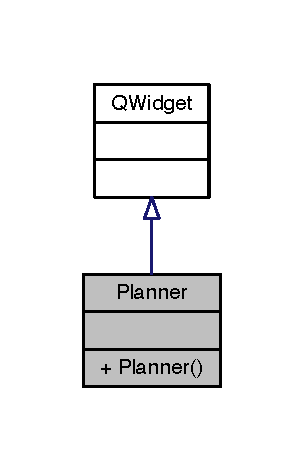
\includegraphics[width=146pt]{dc/d03/class_planner__inherit__graph}
\end{center}
\end{figure}


Samarbejdsdiagram for Planner\+:
\nopagebreak
\begin{figure}[H]
\begin{center}
\leavevmode
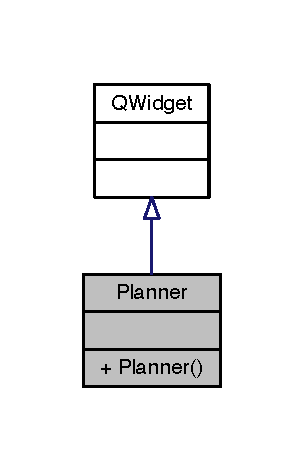
\includegraphics[width=146pt]{da/d60/class_planner__coll__graph}
\end{center}
\end{figure}
\subsubsection*{Offentlige metoder}
\begin{DoxyCompactItemize}
\item 
\hyperlink{class_planner_a8c2728f8232cd88ab7d95375dc3ad4af}{Planner} (\hyperlink{class_q_widget}{Q\+Widget} $\ast$parent=0)
\end{DoxyCompactItemize}


\subsubsection{Detaljeret beskrivelse}


Defineret på linje 6 i filen planner.\+h.



\subsubsection{Dokumentation af konstruktører og destruktører}
\index{Planner@{Planner}!Planner@{Planner}}
\index{Planner@{Planner}!Planner@{Planner}}
\paragraph[{\texorpdfstring{Planner(\+Q\+Widget $\ast$parent=0)}{Planner(QWidget *parent=0)}}]{\setlength{\rightskip}{0pt plus 5cm}{\bf Planner} (
\begin{DoxyParamCaption}
\item[{{\bf Q\+Widget} $\ast$}]{parent = {\ttfamily 0}}
\end{DoxyParamCaption}
)\hspace{0.3cm}{\ttfamily [explicit]}}\hypertarget{class_planner_a8c2728f8232cd88ab7d95375dc3ad4af}{}\label{class_planner_a8c2728f8232cd88ab7d95375dc3ad4af}


Dokumentationen for denne klasse blev genereret ud fra filen\+:\begin{DoxyCompactItemize}
\item 
\hyperlink{planner_8h}{planner.\+h}\end{DoxyCompactItemize}

\hypertarget{class_planner_dialog}{}\subsection{Planner\+Dialog Klasse-\/reference}
\label{class_planner_dialog}\index{Planner\+Dialog@{Planner\+Dialog}}


{\ttfamily \#include $<$plannerdialog.\+h$>$}



Stamtræ for Planner\+Dialog\+:
\nopagebreak
\begin{figure}[H]
\begin{center}
\leavevmode
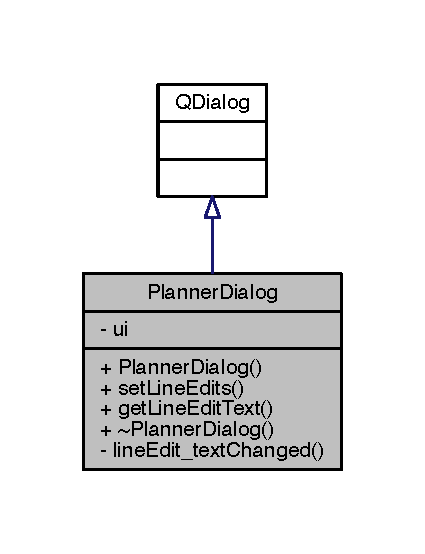
\includegraphics[width=204pt]{d8/de5/class_planner_dialog__inherit__graph}
\end{center}
\end{figure}


Samarbejdsdiagram for Planner\+Dialog\+:
\nopagebreak
\begin{figure}[H]
\begin{center}
\leavevmode
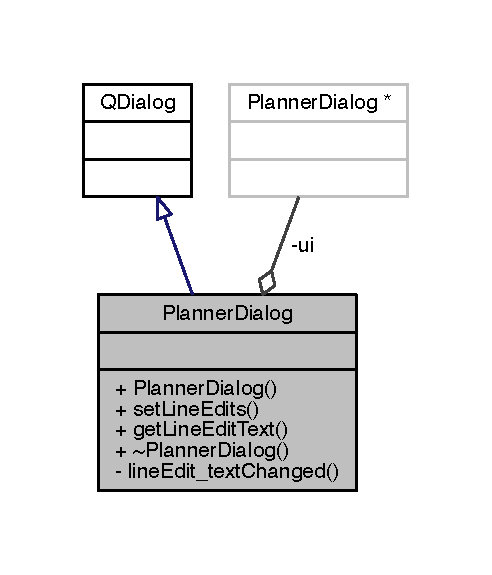
\includegraphics[width=236pt]{d2/d03/class_planner_dialog__coll__graph}
\end{center}
\end{figure}
\subsubsection*{Offentlige metoder}
\begin{DoxyCompactItemize}
\item 
\hyperlink{class_planner_dialog_a2f5d2ba887c4b70a3f28d78955aa1536}{Planner\+Dialog} (\hyperlink{class_q_widget}{Q\+Widget} $\ast$parent=0)
\item 
void \hyperlink{class_planner_dialog_a83441caf32a5806cfbb5f0796065d352}{set\+Line\+Edits} (Q\+String plan)
\item 
Q\+String \hyperlink{class_planner_dialog_a7c9482ec9a38bf3d4a90dadf6dc3f572}{get\+Line\+Edit\+Text} () const 
\item 
\hyperlink{class_planner_dialog_a24842220c2a6f2dde621b5ef0bde0217}{$\sim$\+Planner\+Dialog} ()
\end{DoxyCompactItemize}
\subsubsection*{Private slots}
\begin{DoxyCompactItemize}
\item 
void \hyperlink{class_planner_dialog_ad59b9da096cc8570abaf6156512b10a8}{line\+Edit\+\_\+text\+Changed} ()
\end{DoxyCompactItemize}
\subsubsection*{Private attributter}
\begin{DoxyCompactItemize}
\item 
Ui\+::\+Planner\+Dialog $\ast$ \hyperlink{class_planner_dialog_a230ac8ce9ff95f43557ac406c5e4fcc6}{ui}
\end{DoxyCompactItemize}


\subsubsection{Detaljeret beskrivelse}
\begin{DoxyAuthor}{Forfatter}
Victor Busk (\href{mailto:201409557@post.au.dk}{\tt 201409557@post.\+au.\+dk}) 
\end{DoxyAuthor}


Defineret på linje 18 i filen plannerdialog.\+h.



\subsubsection{Dokumentation af konstruktører og destruktører}
\index{Planner\+Dialog@{Planner\+Dialog}!Planner\+Dialog@{Planner\+Dialog}}
\index{Planner\+Dialog@{Planner\+Dialog}!Planner\+Dialog@{Planner\+Dialog}}
\paragraph[{\texorpdfstring{Planner\+Dialog(\+Q\+Widget $\ast$parent=0)}{PlannerDialog(QWidget *parent=0)}}]{\setlength{\rightskip}{0pt plus 5cm}{\bf Planner\+Dialog} (
\begin{DoxyParamCaption}
\item[{{\bf Q\+Widget} $\ast$}]{parent = {\ttfamily 0}}
\end{DoxyParamCaption}
)\hspace{0.3cm}{\ttfamily [explicit]}}\hypertarget{class_planner_dialog_a2f5d2ba887c4b70a3f28d78955aa1536}{}\label{class_planner_dialog_a2f5d2ba887c4b70a3f28d78955aa1536}
\index{Planner\+Dialog@{Planner\+Dialog}!````~Planner\+Dialog@{$\sim$\+Planner\+Dialog}}
\index{````~Planner\+Dialog@{$\sim$\+Planner\+Dialog}!Planner\+Dialog@{Planner\+Dialog}}
\paragraph[{\texorpdfstring{$\sim$\+Planner\+Dialog()}{~PlannerDialog()}}]{\setlength{\rightskip}{0pt plus 5cm}$\sim${\bf Planner\+Dialog} (
\begin{DoxyParamCaption}
{}
\end{DoxyParamCaption}
)}\hypertarget{class_planner_dialog_a24842220c2a6f2dde621b5ef0bde0217}{}\label{class_planner_dialog_a24842220c2a6f2dde621b5ef0bde0217}


\subsubsection{Dokumentation af medlemsfunktioner}
\index{Planner\+Dialog@{Planner\+Dialog}!get\+Line\+Edit\+Text@{get\+Line\+Edit\+Text}}
\index{get\+Line\+Edit\+Text@{get\+Line\+Edit\+Text}!Planner\+Dialog@{Planner\+Dialog}}
\paragraph[{\texorpdfstring{get\+Line\+Edit\+Text() const }{getLineEditText() const }}]{\setlength{\rightskip}{0pt plus 5cm}Q\+String get\+Line\+Edit\+Text (
\begin{DoxyParamCaption}
{}
\end{DoxyParamCaption}
) const}\hypertarget{class_planner_dialog_a7c9482ec9a38bf3d4a90dadf6dc3f572}{}\label{class_planner_dialog_a7c9482ec9a38bf3d4a90dadf6dc3f572}
\index{Planner\+Dialog@{Planner\+Dialog}!line\+Edit\+\_\+text\+Changed@{line\+Edit\+\_\+text\+Changed}}
\index{line\+Edit\+\_\+text\+Changed@{line\+Edit\+\_\+text\+Changed}!Planner\+Dialog@{Planner\+Dialog}}
\paragraph[{\texorpdfstring{line\+Edit\+\_\+text\+Changed}{lineEdit_textChanged}}]{\setlength{\rightskip}{0pt plus 5cm}void line\+Edit\+\_\+text\+Changed (
\begin{DoxyParamCaption}
{}
\end{DoxyParamCaption}
)\hspace{0.3cm}{\ttfamily [private]}, {\ttfamily [slot]}}\hypertarget{class_planner_dialog_ad59b9da096cc8570abaf6156512b10a8}{}\label{class_planner_dialog_ad59b9da096cc8570abaf6156512b10a8}
\index{Planner\+Dialog@{Planner\+Dialog}!set\+Line\+Edits@{set\+Line\+Edits}}
\index{set\+Line\+Edits@{set\+Line\+Edits}!Planner\+Dialog@{Planner\+Dialog}}
\paragraph[{\texorpdfstring{set\+Line\+Edits(\+Q\+String plan)}{setLineEdits(QString plan)}}]{\setlength{\rightskip}{0pt plus 5cm}void set\+Line\+Edits (
\begin{DoxyParamCaption}
\item[{Q\+String}]{plan}
\end{DoxyParamCaption}
)}\hypertarget{class_planner_dialog_a83441caf32a5806cfbb5f0796065d352}{}\label{class_planner_dialog_a83441caf32a5806cfbb5f0796065d352}


\subsubsection{Felt-\/dokumentation}
\index{Planner\+Dialog@{Planner\+Dialog}!ui@{ui}}
\index{ui@{ui}!Planner\+Dialog@{Planner\+Dialog}}
\paragraph[{\texorpdfstring{ui}{ui}}]{\setlength{\rightskip}{0pt plus 5cm}Ui\+::\+Planner\+Dialog$\ast$ ui\hspace{0.3cm}{\ttfamily [private]}}\hypertarget{class_planner_dialog_a230ac8ce9ff95f43557ac406c5e4fcc6}{}\label{class_planner_dialog_a230ac8ce9ff95f43557ac406c5e4fcc6}


Defineret på linje 34 i filen plannerdialog.\+h.



Dokumentationen for denne klasse blev genereret ud fra filen\+:\begin{DoxyCompactItemize}
\item 
\hyperlink{plannerdialog_8h}{plannerdialog.\+h}\end{DoxyCompactItemize}

\hypertarget{class_q_dialog}{}\subsection{Q\+Dialog Klasse-\/reference}
\label{class_q_dialog}\index{Q\+Dialog@{Q\+Dialog}}


Stamtræ for Q\+Dialog\+:
\nopagebreak
\begin{figure}[H]
\begin{center}
\leavevmode
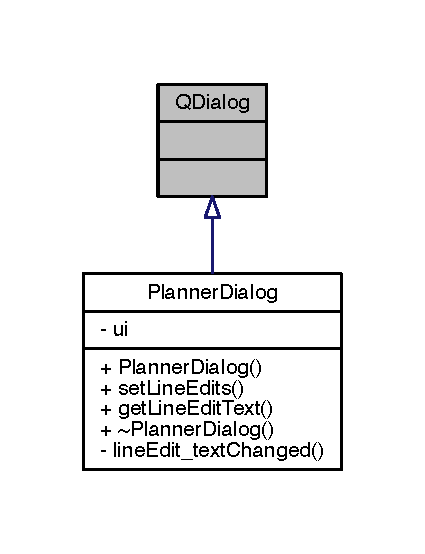
\includegraphics[width=204pt]{df/d5b/class_q_dialog__inherit__graph}
\end{center}
\end{figure}


Samarbejdsdiagram for Q\+Dialog\+:
\nopagebreak
\begin{figure}[H]
\begin{center}
\leavevmode
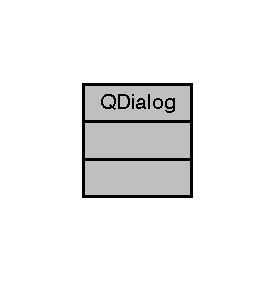
\includegraphics[width=132pt]{de/d99/class_q_dialog__coll__graph}
\end{center}
\end{figure}


Dokumentationen for denne klasse blev genereret ud fra filen\+:\begin{DoxyCompactItemize}
\item 
\hyperlink{plannerdialog_8h}{plannerdialog.\+h}\end{DoxyCompactItemize}

\hypertarget{class_q_tab_widget}{}\subsection{Q\+Tab\+Widget Klasse-\/reference}
\label{class_q_tab_widget}\index{Q\+Tab\+Widget@{Q\+Tab\+Widget}}


Stamtræ for Q\+Tab\+Widget\+:
\nopagebreak
\begin{figure}[H]
\begin{center}
\leavevmode
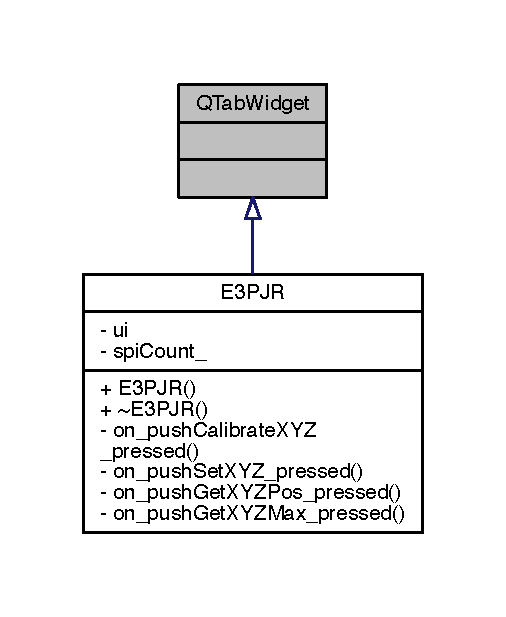
\includegraphics[width=243pt]{class_q_tab_widget__inherit__graph}
\end{center}
\end{figure}


Samarbejdsdiagram for Q\+Tab\+Widget\+:
\nopagebreak
\begin{figure}[H]
\begin{center}
\leavevmode
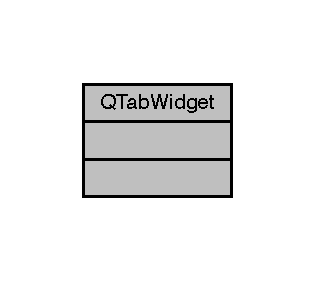
\includegraphics[width=151pt]{class_q_tab_widget__coll__graph}
\end{center}
\end{figure}


Dokumentationen for denne klasse blev genereret ud fra filen\+:\begin{DoxyCompactItemize}
\item 
\hyperlink{e3pjr_8h}{e3pjr.\+h}\end{DoxyCompactItemize}

\hypertarget{class_q_virtual_keyboard}{}\subsection{Q\+Virtual\+Keyboard Klasse-\/reference}
\label{class_q_virtual_keyboard}\index{Q\+Virtual\+Keyboard@{Q\+Virtual\+Keyboard}}


{\ttfamily \#include $<$Q\+Virtual\+Keyboard.\+h$>$}



Stamtræ for Q\+Virtual\+Keyboard\+:\nopagebreak
\begin{figure}[H]
\begin{center}
\leavevmode
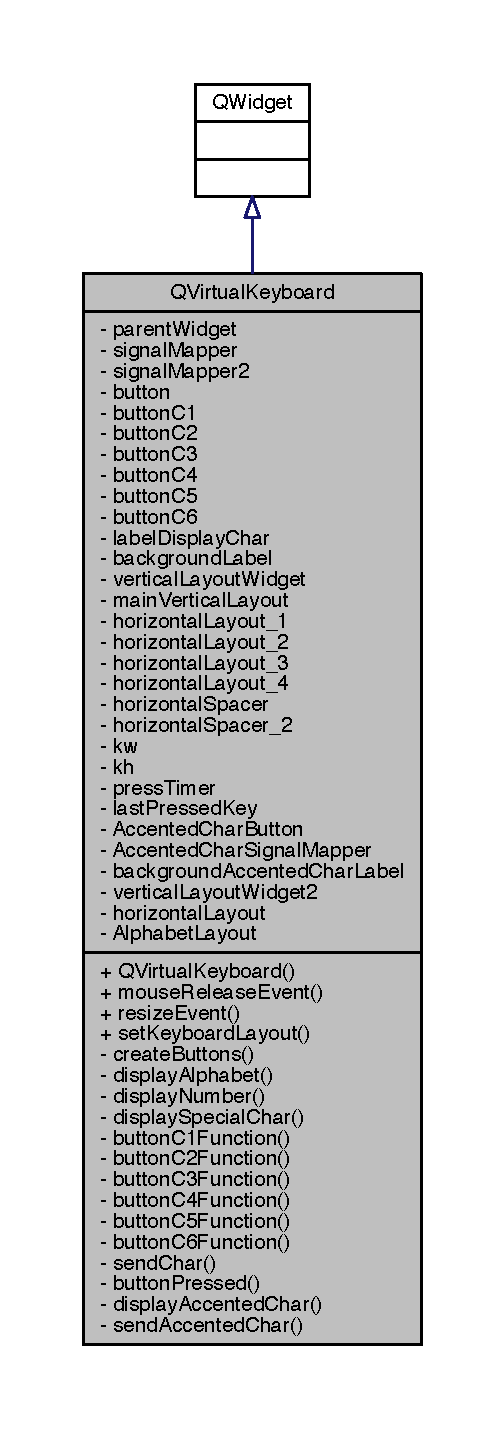
\includegraphics[height=550pt]{db/da8/class_q_virtual_keyboard__inherit__graph}
\end{center}
\end{figure}


Samarbejdsdiagram for Q\+Virtual\+Keyboard\+:\nopagebreak
\begin{figure}[H]
\begin{center}
\leavevmode
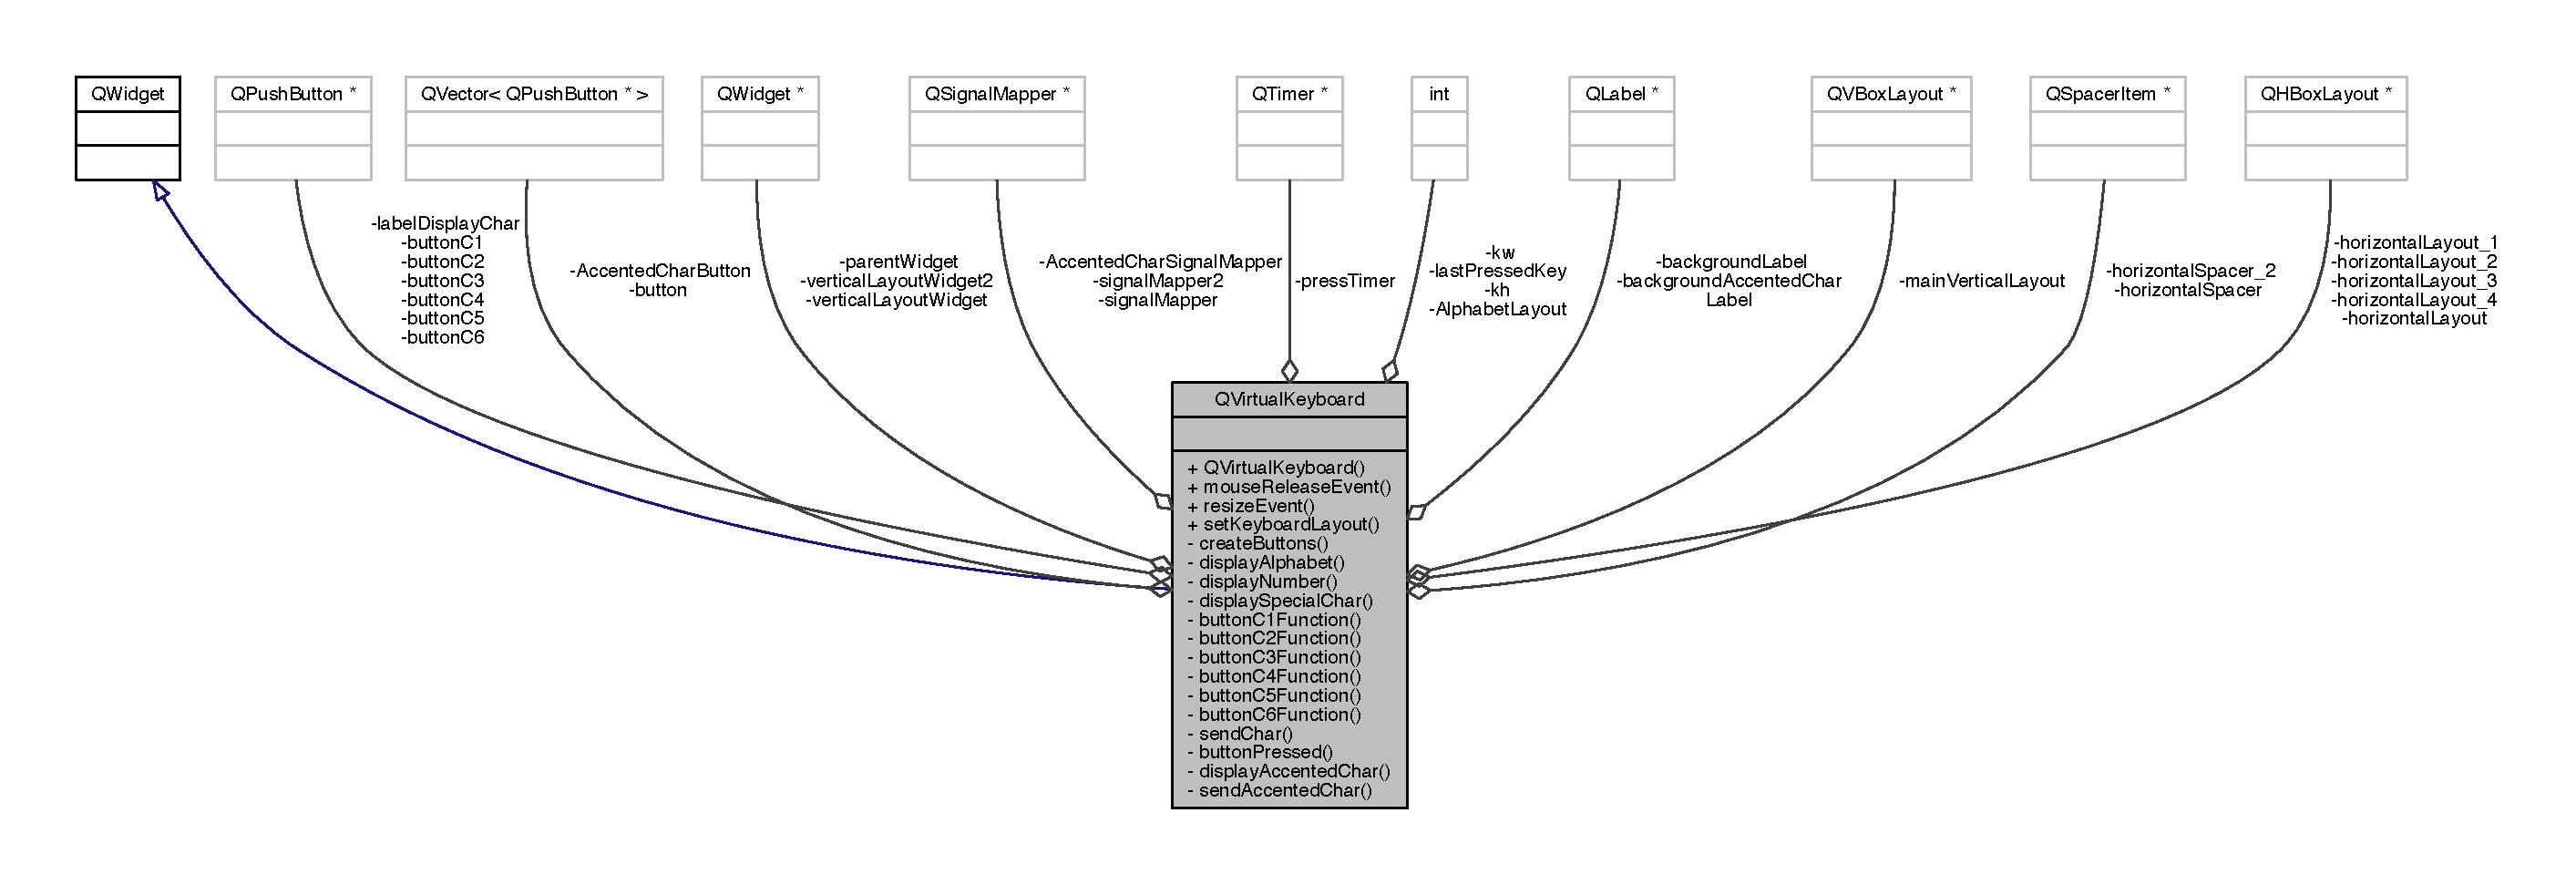
\includegraphics[width=350pt]{d2/d1a/class_q_virtual_keyboard__coll__graph}
\end{center}
\end{figure}
\subsubsection*{Offentlige metoder}
\begin{DoxyCompactItemize}
\item 
\hyperlink{class_q_virtual_keyboard_afc7b26ae7bb5c5dbf3180e1772e93541}{Q\+Virtual\+Keyboard} (\hyperlink{class_q_widget}{Q\+Widget} $\ast$parent=0)
\item 
void \hyperlink{class_q_virtual_keyboard_a35226f6549add1ff837c65888fcd00fc}{mouse\+Release\+Event} (Q\+Mouse\+Event $\ast$event)
\item 
void \hyperlink{class_q_virtual_keyboard_a6fbc07cec19868c41d513b9ef8343e9a}{resize\+Event} (Q\+Resize\+Event $\ast$event)
\item 
void \hyperlink{class_q_virtual_keyboard_a246743b8e5e49a9faaa175cd15dd6f4c}{set\+Keyboard\+Layout} (int layout)
\end{DoxyCompactItemize}
\subsubsection*{Private slots}
\begin{DoxyCompactItemize}
\item 
void \hyperlink{class_q_virtual_keyboard_a40014922c17ece577edf6192e7ddf060}{create\+Buttons} (void)
\item 
void \hyperlink{class_q_virtual_keyboard_aa8b07e67a633d6bb80a22cbf511993f8}{display\+Alphabet} (void)
\item 
void \hyperlink{class_q_virtual_keyboard_a55b57aad2bd2229accaf251bc9048cec}{display\+Number} (void)
\item 
void \hyperlink{class_q_virtual_keyboard_a2b1d480773f837bd0f781399e6d7db59}{display\+Special\+Char} (void)
\item 
void \hyperlink{class_q_virtual_keyboard_ad5a6d0ff933a561b273549b78c31fd4e}{button\+C1\+Function} (void)
\item 
void \hyperlink{class_q_virtual_keyboard_a9e926203d39d233505ecbc67565701d9}{button\+C2\+Function} (void)
\item 
void \hyperlink{class_q_virtual_keyboard_a0132f341d2cad297611d6aededcdd152}{button\+C3\+Function} (void)
\item 
void \hyperlink{class_q_virtual_keyboard_a5be7b200eacaca5ca767c2e4efd0cb64}{button\+C4\+Function} (void)
\item 
void \hyperlink{class_q_virtual_keyboard_a1a7cc07beec5d32833426a6b3d2ba01a}{button\+C5\+Function} (void)
\item 
void \hyperlink{class_q_virtual_keyboard_af4db06bec2ed47409e9ee9743910c010}{button\+C6\+Function} (void)
\item 
void \hyperlink{class_q_virtual_keyboard_af5a2602fcde26706582fb50c3b28b35b}{send\+Char} (int index\+Of\+Char\+To\+Send)
\item 
void \hyperlink{class_q_virtual_keyboard_a8d59c301c476f98ef168b4da7a30bacf}{button\+Pressed} (int index\+Of\+Char\+To\+Send)
\item 
void \hyperlink{class_q_virtual_keyboard_a6407d7d230617ec40b905f1cc6d7afae}{display\+Accented\+Char} (void)
\item 
void \hyperlink{class_q_virtual_keyboard_a82af8c33e832f7c8173b739a03919d95}{send\+Accented\+Char} (int index\+Of\+Char\+To\+Send)
\end{DoxyCompactItemize}
\subsubsection*{Private attributter}
\begin{DoxyCompactItemize}
\item 
\hyperlink{class_q_widget}{Q\+Widget} $\ast$ \hyperlink{class_q_virtual_keyboard_ad9c9372b637d19e1d7e35c44eef6e3e7}{parent\+Widget}
\item 
Q\+Signal\+Mapper $\ast$ \hyperlink{class_q_virtual_keyboard_aaa72fcbe4b8eac04110e709e5876436b}{signal\+Mapper}
\item 
Q\+Signal\+Mapper $\ast$ \hyperlink{class_q_virtual_keyboard_a4696f23cc6529fba639a8f52679ba8dd}{signal\+Mapper2}
\item 
Q\+Vector$<$ Q\+Push\+Button $\ast$ $>$ \hyperlink{class_q_virtual_keyboard_aceb8c4f9d7381faae49bbc8638e4f286}{button}
\item 
Q\+Push\+Button $\ast$ \hyperlink{class_q_virtual_keyboard_abede25384f9be8870ef541a31a27ccfc}{button\+C1}
\item 
Q\+Push\+Button $\ast$ \hyperlink{class_q_virtual_keyboard_a7f0959a9c59da7940cc052ea51626c5f}{button\+C2}
\item 
Q\+Push\+Button $\ast$ \hyperlink{class_q_virtual_keyboard_ab33b8e12f4e396eed1b96cb46dc890fb}{button\+C3}
\item 
Q\+Push\+Button $\ast$ \hyperlink{class_q_virtual_keyboard_a25f42c686bab18c2fbe87cf1f49dcde5}{button\+C4}
\item 
Q\+Push\+Button $\ast$ \hyperlink{class_q_virtual_keyboard_a7221321ae78fe3e486e098a1e44f34b0}{button\+C5}
\item 
Q\+Push\+Button $\ast$ \hyperlink{class_q_virtual_keyboard_ac332f23e9b221714f422087d2d87d9b6}{button\+C6}
\item 
Q\+Push\+Button $\ast$ \hyperlink{class_q_virtual_keyboard_a2230006aad7be0bfd701328870f4dcee}{label\+Display\+Char}
\item 
Q\+Label $\ast$ \hyperlink{class_q_virtual_keyboard_a2eb3cbd95ab4f4c8930d6e5174eba3af}{background\+Label}
\item 
\hyperlink{class_q_widget}{Q\+Widget} $\ast$ \hyperlink{class_q_virtual_keyboard_a4dab2ee47678bbea22fe10267a009293}{vertical\+Layout\+Widget}
\item 
Q\+V\+Box\+Layout $\ast$ \hyperlink{class_q_virtual_keyboard_aad608b448bdf0d3b90753859aab1f21b}{main\+Vertical\+Layout}
\item 
Q\+H\+Box\+Layout $\ast$ \hyperlink{class_q_virtual_keyboard_a33382d1f071315a4549f47f72121956a}{horizontal\+Layout\+\_\+1}
\item 
Q\+H\+Box\+Layout $\ast$ \hyperlink{class_q_virtual_keyboard_a535a43287b7a5605cfc11580d146d3fb}{horizontal\+Layout\+\_\+2}
\item 
Q\+H\+Box\+Layout $\ast$ \hyperlink{class_q_virtual_keyboard_af1b2167ad3027fe2c2328701164e54ec}{horizontal\+Layout\+\_\+3}
\item 
Q\+H\+Box\+Layout $\ast$ \hyperlink{class_q_virtual_keyboard_aeb3eff1a8b0673c92f1ed957263d272b}{horizontal\+Layout\+\_\+4}
\item 
Q\+Spacer\+Item $\ast$ \hyperlink{class_q_virtual_keyboard_a7e1d33086b18025c1f6a73ee4b080442}{horizontal\+Spacer}
\item 
Q\+Spacer\+Item $\ast$ \hyperlink{class_q_virtual_keyboard_ad8c8a25c788a6f06d18143815745542c}{horizontal\+Spacer\+\_\+2}
\item 
int \hyperlink{class_q_virtual_keyboard_a5a953764bcaf68b8491ec52111189e31}{kw}
\item 
int \hyperlink{class_q_virtual_keyboard_ac85dabb3c71c98632f077058f4bbe3c7}{kh}
\item 
Q\+Timer $\ast$ \hyperlink{class_q_virtual_keyboard_a050363eca09454d325785185e147a3b3}{press\+Timer}
\item 
int \hyperlink{class_q_virtual_keyboard_ab0906b0492ca8865fd2db9547599636f}{last\+Pressed\+Key}
\item 
Q\+Vector$<$ Q\+Push\+Button $\ast$ $>$ \hyperlink{class_q_virtual_keyboard_aeeb3a644e1608dbbf2b68462e1615fef}{Accented\+Char\+Button}
\item 
Q\+Signal\+Mapper $\ast$ \hyperlink{class_q_virtual_keyboard_a8d1ccfcfe491a906a540bfc0e7532166}{Accented\+Char\+Signal\+Mapper}
\item 
Q\+Label $\ast$ \hyperlink{class_q_virtual_keyboard_a6853ae9cfabf643af6b7acb814ffa6a1}{background\+Accented\+Char\+Label}
\item 
\hyperlink{class_q_widget}{Q\+Widget} $\ast$ \hyperlink{class_q_virtual_keyboard_a6cae2ca1d83910c66adfc69bc57a770d}{vertical\+Layout\+Widget2}
\item 
Q\+H\+Box\+Layout $\ast$ \hyperlink{class_q_virtual_keyboard_a9ca831b3e7278c1cc7cebba2329486b4}{horizontal\+Layout}
\item 
int \hyperlink{class_q_virtual_keyboard_a5f4c5779dd39f7a3602aed3a8dff9054}{Alphabet\+Layout}
\end{DoxyCompactItemize}


\subsubsection{Detaljeret beskrivelse}


Defineret på linje 28 i filen Q\+Virtual\+Keyboard.\+h.



\subsubsection{Dokumentation af konstruktører og destruktører}
\index{Q\+Virtual\+Keyboard@{Q\+Virtual\+Keyboard}!Q\+Virtual\+Keyboard@{Q\+Virtual\+Keyboard}}
\index{Q\+Virtual\+Keyboard@{Q\+Virtual\+Keyboard}!Q\+Virtual\+Keyboard@{Q\+Virtual\+Keyboard}}
\paragraph[{\texorpdfstring{Q\+Virtual\+Keyboard(\+Q\+Widget $\ast$parent=0)}{QVirtualKeyboard(QWidget *parent=0)}}]{\setlength{\rightskip}{0pt plus 5cm}{\bf Q\+Virtual\+Keyboard} (
\begin{DoxyParamCaption}
\item[{{\bf Q\+Widget} $\ast$}]{parent = {\ttfamily 0}}
\end{DoxyParamCaption}
)}\hypertarget{class_q_virtual_keyboard_afc7b26ae7bb5c5dbf3180e1772e93541}{}\label{class_q_virtual_keyboard_afc7b26ae7bb5c5dbf3180e1772e93541}


\subsubsection{Dokumentation af medlemsfunktioner}
\index{Q\+Virtual\+Keyboard@{Q\+Virtual\+Keyboard}!button\+C1\+Function@{button\+C1\+Function}}
\index{button\+C1\+Function@{button\+C1\+Function}!Q\+Virtual\+Keyboard@{Q\+Virtual\+Keyboard}}
\paragraph[{\texorpdfstring{button\+C1\+Function}{buttonC1Function}}]{\setlength{\rightskip}{0pt plus 5cm}void button\+C1\+Function (
\begin{DoxyParamCaption}
\item[{void}]{}
\end{DoxyParamCaption}
)\hspace{0.3cm}{\ttfamily [private]}, {\ttfamily [slot]}}\hypertarget{class_q_virtual_keyboard_ad5a6d0ff933a561b273549b78c31fd4e}{}\label{class_q_virtual_keyboard_ad5a6d0ff933a561b273549b78c31fd4e}
\index{Q\+Virtual\+Keyboard@{Q\+Virtual\+Keyboard}!button\+C2\+Function@{button\+C2\+Function}}
\index{button\+C2\+Function@{button\+C2\+Function}!Q\+Virtual\+Keyboard@{Q\+Virtual\+Keyboard}}
\paragraph[{\texorpdfstring{button\+C2\+Function}{buttonC2Function}}]{\setlength{\rightskip}{0pt plus 5cm}void button\+C2\+Function (
\begin{DoxyParamCaption}
\item[{void}]{}
\end{DoxyParamCaption}
)\hspace{0.3cm}{\ttfamily [private]}, {\ttfamily [slot]}}\hypertarget{class_q_virtual_keyboard_a9e926203d39d233505ecbc67565701d9}{}\label{class_q_virtual_keyboard_a9e926203d39d233505ecbc67565701d9}
\index{Q\+Virtual\+Keyboard@{Q\+Virtual\+Keyboard}!button\+C3\+Function@{button\+C3\+Function}}
\index{button\+C3\+Function@{button\+C3\+Function}!Q\+Virtual\+Keyboard@{Q\+Virtual\+Keyboard}}
\paragraph[{\texorpdfstring{button\+C3\+Function}{buttonC3Function}}]{\setlength{\rightskip}{0pt plus 5cm}void button\+C3\+Function (
\begin{DoxyParamCaption}
\item[{void}]{}
\end{DoxyParamCaption}
)\hspace{0.3cm}{\ttfamily [private]}, {\ttfamily [slot]}}\hypertarget{class_q_virtual_keyboard_a0132f341d2cad297611d6aededcdd152}{}\label{class_q_virtual_keyboard_a0132f341d2cad297611d6aededcdd152}
\index{Q\+Virtual\+Keyboard@{Q\+Virtual\+Keyboard}!button\+C4\+Function@{button\+C4\+Function}}
\index{button\+C4\+Function@{button\+C4\+Function}!Q\+Virtual\+Keyboard@{Q\+Virtual\+Keyboard}}
\paragraph[{\texorpdfstring{button\+C4\+Function}{buttonC4Function}}]{\setlength{\rightskip}{0pt plus 5cm}void button\+C4\+Function (
\begin{DoxyParamCaption}
\item[{void}]{}
\end{DoxyParamCaption}
)\hspace{0.3cm}{\ttfamily [private]}, {\ttfamily [slot]}}\hypertarget{class_q_virtual_keyboard_a5be7b200eacaca5ca767c2e4efd0cb64}{}\label{class_q_virtual_keyboard_a5be7b200eacaca5ca767c2e4efd0cb64}
\index{Q\+Virtual\+Keyboard@{Q\+Virtual\+Keyboard}!button\+C5\+Function@{button\+C5\+Function}}
\index{button\+C5\+Function@{button\+C5\+Function}!Q\+Virtual\+Keyboard@{Q\+Virtual\+Keyboard}}
\paragraph[{\texorpdfstring{button\+C5\+Function}{buttonC5Function}}]{\setlength{\rightskip}{0pt plus 5cm}void button\+C5\+Function (
\begin{DoxyParamCaption}
\item[{void}]{}
\end{DoxyParamCaption}
)\hspace{0.3cm}{\ttfamily [private]}, {\ttfamily [slot]}}\hypertarget{class_q_virtual_keyboard_a1a7cc07beec5d32833426a6b3d2ba01a}{}\label{class_q_virtual_keyboard_a1a7cc07beec5d32833426a6b3d2ba01a}
\index{Q\+Virtual\+Keyboard@{Q\+Virtual\+Keyboard}!button\+C6\+Function@{button\+C6\+Function}}
\index{button\+C6\+Function@{button\+C6\+Function}!Q\+Virtual\+Keyboard@{Q\+Virtual\+Keyboard}}
\paragraph[{\texorpdfstring{button\+C6\+Function}{buttonC6Function}}]{\setlength{\rightskip}{0pt plus 5cm}void button\+C6\+Function (
\begin{DoxyParamCaption}
\item[{void}]{}
\end{DoxyParamCaption}
)\hspace{0.3cm}{\ttfamily [private]}, {\ttfamily [slot]}}\hypertarget{class_q_virtual_keyboard_af4db06bec2ed47409e9ee9743910c010}{}\label{class_q_virtual_keyboard_af4db06bec2ed47409e9ee9743910c010}
\index{Q\+Virtual\+Keyboard@{Q\+Virtual\+Keyboard}!button\+Pressed@{button\+Pressed}}
\index{button\+Pressed@{button\+Pressed}!Q\+Virtual\+Keyboard@{Q\+Virtual\+Keyboard}}
\paragraph[{\texorpdfstring{button\+Pressed}{buttonPressed}}]{\setlength{\rightskip}{0pt plus 5cm}void button\+Pressed (
\begin{DoxyParamCaption}
\item[{int}]{index\+Of\+Char\+To\+Send}
\end{DoxyParamCaption}
)\hspace{0.3cm}{\ttfamily [private]}, {\ttfamily [slot]}}\hypertarget{class_q_virtual_keyboard_a8d59c301c476f98ef168b4da7a30bacf}{}\label{class_q_virtual_keyboard_a8d59c301c476f98ef168b4da7a30bacf}
\index{Q\+Virtual\+Keyboard@{Q\+Virtual\+Keyboard}!create\+Buttons@{create\+Buttons}}
\index{create\+Buttons@{create\+Buttons}!Q\+Virtual\+Keyboard@{Q\+Virtual\+Keyboard}}
\paragraph[{\texorpdfstring{create\+Buttons}{createButtons}}]{\setlength{\rightskip}{0pt plus 5cm}void create\+Buttons (
\begin{DoxyParamCaption}
\item[{void}]{}
\end{DoxyParamCaption}
)\hspace{0.3cm}{\ttfamily [private]}, {\ttfamily [slot]}}\hypertarget{class_q_virtual_keyboard_a40014922c17ece577edf6192e7ddf060}{}\label{class_q_virtual_keyboard_a40014922c17ece577edf6192e7ddf060}
\index{Q\+Virtual\+Keyboard@{Q\+Virtual\+Keyboard}!display\+Accented\+Char@{display\+Accented\+Char}}
\index{display\+Accented\+Char@{display\+Accented\+Char}!Q\+Virtual\+Keyboard@{Q\+Virtual\+Keyboard}}
\paragraph[{\texorpdfstring{display\+Accented\+Char}{displayAccentedChar}}]{\setlength{\rightskip}{0pt plus 5cm}void display\+Accented\+Char (
\begin{DoxyParamCaption}
\item[{void}]{}
\end{DoxyParamCaption}
)\hspace{0.3cm}{\ttfamily [private]}, {\ttfamily [slot]}}\hypertarget{class_q_virtual_keyboard_a6407d7d230617ec40b905f1cc6d7afae}{}\label{class_q_virtual_keyboard_a6407d7d230617ec40b905f1cc6d7afae}
\index{Q\+Virtual\+Keyboard@{Q\+Virtual\+Keyboard}!display\+Alphabet@{display\+Alphabet}}
\index{display\+Alphabet@{display\+Alphabet}!Q\+Virtual\+Keyboard@{Q\+Virtual\+Keyboard}}
\paragraph[{\texorpdfstring{display\+Alphabet}{displayAlphabet}}]{\setlength{\rightskip}{0pt plus 5cm}void display\+Alphabet (
\begin{DoxyParamCaption}
\item[{void}]{}
\end{DoxyParamCaption}
)\hspace{0.3cm}{\ttfamily [private]}, {\ttfamily [slot]}}\hypertarget{class_q_virtual_keyboard_aa8b07e67a633d6bb80a22cbf511993f8}{}\label{class_q_virtual_keyboard_aa8b07e67a633d6bb80a22cbf511993f8}
\index{Q\+Virtual\+Keyboard@{Q\+Virtual\+Keyboard}!display\+Number@{display\+Number}}
\index{display\+Number@{display\+Number}!Q\+Virtual\+Keyboard@{Q\+Virtual\+Keyboard}}
\paragraph[{\texorpdfstring{display\+Number}{displayNumber}}]{\setlength{\rightskip}{0pt plus 5cm}void display\+Number (
\begin{DoxyParamCaption}
\item[{void}]{}
\end{DoxyParamCaption}
)\hspace{0.3cm}{\ttfamily [private]}, {\ttfamily [slot]}}\hypertarget{class_q_virtual_keyboard_a55b57aad2bd2229accaf251bc9048cec}{}\label{class_q_virtual_keyboard_a55b57aad2bd2229accaf251bc9048cec}
\index{Q\+Virtual\+Keyboard@{Q\+Virtual\+Keyboard}!display\+Special\+Char@{display\+Special\+Char}}
\index{display\+Special\+Char@{display\+Special\+Char}!Q\+Virtual\+Keyboard@{Q\+Virtual\+Keyboard}}
\paragraph[{\texorpdfstring{display\+Special\+Char}{displaySpecialChar}}]{\setlength{\rightskip}{0pt plus 5cm}void display\+Special\+Char (
\begin{DoxyParamCaption}
\item[{void}]{}
\end{DoxyParamCaption}
)\hspace{0.3cm}{\ttfamily [private]}, {\ttfamily [slot]}}\hypertarget{class_q_virtual_keyboard_a2b1d480773f837bd0f781399e6d7db59}{}\label{class_q_virtual_keyboard_a2b1d480773f837bd0f781399e6d7db59}
\index{Q\+Virtual\+Keyboard@{Q\+Virtual\+Keyboard}!mouse\+Release\+Event@{mouse\+Release\+Event}}
\index{mouse\+Release\+Event@{mouse\+Release\+Event}!Q\+Virtual\+Keyboard@{Q\+Virtual\+Keyboard}}
\paragraph[{\texorpdfstring{mouse\+Release\+Event(\+Q\+Mouse\+Event $\ast$event)}{mouseReleaseEvent(QMouseEvent *event)}}]{\setlength{\rightskip}{0pt plus 5cm}void mouse\+Release\+Event (
\begin{DoxyParamCaption}
\item[{Q\+Mouse\+Event $\ast$}]{event}
\end{DoxyParamCaption}
)}\hypertarget{class_q_virtual_keyboard_a35226f6549add1ff837c65888fcd00fc}{}\label{class_q_virtual_keyboard_a35226f6549add1ff837c65888fcd00fc}
\index{Q\+Virtual\+Keyboard@{Q\+Virtual\+Keyboard}!resize\+Event@{resize\+Event}}
\index{resize\+Event@{resize\+Event}!Q\+Virtual\+Keyboard@{Q\+Virtual\+Keyboard}}
\paragraph[{\texorpdfstring{resize\+Event(\+Q\+Resize\+Event $\ast$event)}{resizeEvent(QResizeEvent *event)}}]{\setlength{\rightskip}{0pt plus 5cm}void resize\+Event (
\begin{DoxyParamCaption}
\item[{Q\+Resize\+Event $\ast$}]{event}
\end{DoxyParamCaption}
)}\hypertarget{class_q_virtual_keyboard_a6fbc07cec19868c41d513b9ef8343e9a}{}\label{class_q_virtual_keyboard_a6fbc07cec19868c41d513b9ef8343e9a}
\index{Q\+Virtual\+Keyboard@{Q\+Virtual\+Keyboard}!send\+Accented\+Char@{send\+Accented\+Char}}
\index{send\+Accented\+Char@{send\+Accented\+Char}!Q\+Virtual\+Keyboard@{Q\+Virtual\+Keyboard}}
\paragraph[{\texorpdfstring{send\+Accented\+Char}{sendAccentedChar}}]{\setlength{\rightskip}{0pt plus 5cm}void send\+Accented\+Char (
\begin{DoxyParamCaption}
\item[{int}]{index\+Of\+Char\+To\+Send}
\end{DoxyParamCaption}
)\hspace{0.3cm}{\ttfamily [private]}, {\ttfamily [slot]}}\hypertarget{class_q_virtual_keyboard_a82af8c33e832f7c8173b739a03919d95}{}\label{class_q_virtual_keyboard_a82af8c33e832f7c8173b739a03919d95}
\index{Q\+Virtual\+Keyboard@{Q\+Virtual\+Keyboard}!send\+Char@{send\+Char}}
\index{send\+Char@{send\+Char}!Q\+Virtual\+Keyboard@{Q\+Virtual\+Keyboard}}
\paragraph[{\texorpdfstring{send\+Char}{sendChar}}]{\setlength{\rightskip}{0pt plus 5cm}void send\+Char (
\begin{DoxyParamCaption}
\item[{int}]{index\+Of\+Char\+To\+Send}
\end{DoxyParamCaption}
)\hspace{0.3cm}{\ttfamily [private]}, {\ttfamily [slot]}}\hypertarget{class_q_virtual_keyboard_af5a2602fcde26706582fb50c3b28b35b}{}\label{class_q_virtual_keyboard_af5a2602fcde26706582fb50c3b28b35b}
\index{Q\+Virtual\+Keyboard@{Q\+Virtual\+Keyboard}!set\+Keyboard\+Layout@{set\+Keyboard\+Layout}}
\index{set\+Keyboard\+Layout@{set\+Keyboard\+Layout}!Q\+Virtual\+Keyboard@{Q\+Virtual\+Keyboard}}
\paragraph[{\texorpdfstring{set\+Keyboard\+Layout(int layout)}{setKeyboardLayout(int layout)}}]{\setlength{\rightskip}{0pt plus 5cm}void set\+Keyboard\+Layout (
\begin{DoxyParamCaption}
\item[{int}]{layout}
\end{DoxyParamCaption}
)}\hypertarget{class_q_virtual_keyboard_a246743b8e5e49a9faaa175cd15dd6f4c}{}\label{class_q_virtual_keyboard_a246743b8e5e49a9faaa175cd15dd6f4c}


\subsubsection{Felt-\/dokumentation}
\index{Q\+Virtual\+Keyboard@{Q\+Virtual\+Keyboard}!Accented\+Char\+Button@{Accented\+Char\+Button}}
\index{Accented\+Char\+Button@{Accented\+Char\+Button}!Q\+Virtual\+Keyboard@{Q\+Virtual\+Keyboard}}
\paragraph[{\texorpdfstring{Accented\+Char\+Button}{AccentedCharButton}}]{\setlength{\rightskip}{0pt plus 5cm}Q\+Vector$<$Q\+Push\+Button $\ast$$>$ Accented\+Char\+Button\hspace{0.3cm}{\ttfamily [private]}}\hypertarget{class_q_virtual_keyboard_aeeb3a644e1608dbbf2b68462e1615fef}{}\label{class_q_virtual_keyboard_aeeb3a644e1608dbbf2b68462e1615fef}


Defineret på linje 99 i filen Q\+Virtual\+Keyboard.\+h.

\index{Q\+Virtual\+Keyboard@{Q\+Virtual\+Keyboard}!Accented\+Char\+Signal\+Mapper@{Accented\+Char\+Signal\+Mapper}}
\index{Accented\+Char\+Signal\+Mapper@{Accented\+Char\+Signal\+Mapper}!Q\+Virtual\+Keyboard@{Q\+Virtual\+Keyboard}}
\paragraph[{\texorpdfstring{Accented\+Char\+Signal\+Mapper}{AccentedCharSignalMapper}}]{\setlength{\rightskip}{0pt plus 5cm}Q\+Signal\+Mapper$\ast$ Accented\+Char\+Signal\+Mapper\hspace{0.3cm}{\ttfamily [private]}}\hypertarget{class_q_virtual_keyboard_a8d1ccfcfe491a906a540bfc0e7532166}{}\label{class_q_virtual_keyboard_a8d1ccfcfe491a906a540bfc0e7532166}


Defineret på linje 100 i filen Q\+Virtual\+Keyboard.\+h.

\index{Q\+Virtual\+Keyboard@{Q\+Virtual\+Keyboard}!Alphabet\+Layout@{Alphabet\+Layout}}
\index{Alphabet\+Layout@{Alphabet\+Layout}!Q\+Virtual\+Keyboard@{Q\+Virtual\+Keyboard}}
\paragraph[{\texorpdfstring{Alphabet\+Layout}{AlphabetLayout}}]{\setlength{\rightskip}{0pt plus 5cm}int Alphabet\+Layout\hspace{0.3cm}{\ttfamily [private]}}\hypertarget{class_q_virtual_keyboard_a5f4c5779dd39f7a3602aed3a8dff9054}{}\label{class_q_virtual_keyboard_a5f4c5779dd39f7a3602aed3a8dff9054}


Defineret på linje 107 i filen Q\+Virtual\+Keyboard.\+h.

\index{Q\+Virtual\+Keyboard@{Q\+Virtual\+Keyboard}!background\+Accented\+Char\+Label@{background\+Accented\+Char\+Label}}
\index{background\+Accented\+Char\+Label@{background\+Accented\+Char\+Label}!Q\+Virtual\+Keyboard@{Q\+Virtual\+Keyboard}}
\paragraph[{\texorpdfstring{background\+Accented\+Char\+Label}{backgroundAccentedCharLabel}}]{\setlength{\rightskip}{0pt plus 5cm}Q\+Label$\ast$ background\+Accented\+Char\+Label\hspace{0.3cm}{\ttfamily [private]}}\hypertarget{class_q_virtual_keyboard_a6853ae9cfabf643af6b7acb814ffa6a1}{}\label{class_q_virtual_keyboard_a6853ae9cfabf643af6b7acb814ffa6a1}


Defineret på linje 102 i filen Q\+Virtual\+Keyboard.\+h.

\index{Q\+Virtual\+Keyboard@{Q\+Virtual\+Keyboard}!background\+Label@{background\+Label}}
\index{background\+Label@{background\+Label}!Q\+Virtual\+Keyboard@{Q\+Virtual\+Keyboard}}
\paragraph[{\texorpdfstring{background\+Label}{backgroundLabel}}]{\setlength{\rightskip}{0pt plus 5cm}Q\+Label$\ast$ background\+Label\hspace{0.3cm}{\ttfamily [private]}}\hypertarget{class_q_virtual_keyboard_a2eb3cbd95ab4f4c8930d6e5174eba3af}{}\label{class_q_virtual_keyboard_a2eb3cbd95ab4f4c8930d6e5174eba3af}


Defineret på linje 81 i filen Q\+Virtual\+Keyboard.\+h.

\index{Q\+Virtual\+Keyboard@{Q\+Virtual\+Keyboard}!button@{button}}
\index{button@{button}!Q\+Virtual\+Keyboard@{Q\+Virtual\+Keyboard}}
\paragraph[{\texorpdfstring{button}{button}}]{\setlength{\rightskip}{0pt plus 5cm}Q\+Vector$<$Q\+Push\+Button $\ast$$>$ button\hspace{0.3cm}{\ttfamily [private]}}\hypertarget{class_q_virtual_keyboard_aceb8c4f9d7381faae49bbc8638e4f286}{}\label{class_q_virtual_keyboard_aceb8c4f9d7381faae49bbc8638e4f286}


Defineret på linje 70 i filen Q\+Virtual\+Keyboard.\+h.

\index{Q\+Virtual\+Keyboard@{Q\+Virtual\+Keyboard}!button\+C1@{button\+C1}}
\index{button\+C1@{button\+C1}!Q\+Virtual\+Keyboard@{Q\+Virtual\+Keyboard}}
\paragraph[{\texorpdfstring{button\+C1}{buttonC1}}]{\setlength{\rightskip}{0pt plus 5cm}Q\+Push\+Button$\ast$ button\+C1\hspace{0.3cm}{\ttfamily [private]}}\hypertarget{class_q_virtual_keyboard_abede25384f9be8870ef541a31a27ccfc}{}\label{class_q_virtual_keyboard_abede25384f9be8870ef541a31a27ccfc}


Defineret på linje 72 i filen Q\+Virtual\+Keyboard.\+h.

\index{Q\+Virtual\+Keyboard@{Q\+Virtual\+Keyboard}!button\+C2@{button\+C2}}
\index{button\+C2@{button\+C2}!Q\+Virtual\+Keyboard@{Q\+Virtual\+Keyboard}}
\paragraph[{\texorpdfstring{button\+C2}{buttonC2}}]{\setlength{\rightskip}{0pt plus 5cm}Q\+Push\+Button$\ast$ button\+C2\hspace{0.3cm}{\ttfamily [private]}}\hypertarget{class_q_virtual_keyboard_a7f0959a9c59da7940cc052ea51626c5f}{}\label{class_q_virtual_keyboard_a7f0959a9c59da7940cc052ea51626c5f}


Defineret på linje 73 i filen Q\+Virtual\+Keyboard.\+h.

\index{Q\+Virtual\+Keyboard@{Q\+Virtual\+Keyboard}!button\+C3@{button\+C3}}
\index{button\+C3@{button\+C3}!Q\+Virtual\+Keyboard@{Q\+Virtual\+Keyboard}}
\paragraph[{\texorpdfstring{button\+C3}{buttonC3}}]{\setlength{\rightskip}{0pt plus 5cm}Q\+Push\+Button$\ast$ button\+C3\hspace{0.3cm}{\ttfamily [private]}}\hypertarget{class_q_virtual_keyboard_ab33b8e12f4e396eed1b96cb46dc890fb}{}\label{class_q_virtual_keyboard_ab33b8e12f4e396eed1b96cb46dc890fb}


Defineret på linje 74 i filen Q\+Virtual\+Keyboard.\+h.

\index{Q\+Virtual\+Keyboard@{Q\+Virtual\+Keyboard}!button\+C4@{button\+C4}}
\index{button\+C4@{button\+C4}!Q\+Virtual\+Keyboard@{Q\+Virtual\+Keyboard}}
\paragraph[{\texorpdfstring{button\+C4}{buttonC4}}]{\setlength{\rightskip}{0pt plus 5cm}Q\+Push\+Button$\ast$ button\+C4\hspace{0.3cm}{\ttfamily [private]}}\hypertarget{class_q_virtual_keyboard_a25f42c686bab18c2fbe87cf1f49dcde5}{}\label{class_q_virtual_keyboard_a25f42c686bab18c2fbe87cf1f49dcde5}


Defineret på linje 75 i filen Q\+Virtual\+Keyboard.\+h.

\index{Q\+Virtual\+Keyboard@{Q\+Virtual\+Keyboard}!button\+C5@{button\+C5}}
\index{button\+C5@{button\+C5}!Q\+Virtual\+Keyboard@{Q\+Virtual\+Keyboard}}
\paragraph[{\texorpdfstring{button\+C5}{buttonC5}}]{\setlength{\rightskip}{0pt plus 5cm}Q\+Push\+Button$\ast$ button\+C5\hspace{0.3cm}{\ttfamily [private]}}\hypertarget{class_q_virtual_keyboard_a7221321ae78fe3e486e098a1e44f34b0}{}\label{class_q_virtual_keyboard_a7221321ae78fe3e486e098a1e44f34b0}


Defineret på linje 76 i filen Q\+Virtual\+Keyboard.\+h.

\index{Q\+Virtual\+Keyboard@{Q\+Virtual\+Keyboard}!button\+C6@{button\+C6}}
\index{button\+C6@{button\+C6}!Q\+Virtual\+Keyboard@{Q\+Virtual\+Keyboard}}
\paragraph[{\texorpdfstring{button\+C6}{buttonC6}}]{\setlength{\rightskip}{0pt plus 5cm}Q\+Push\+Button$\ast$ button\+C6\hspace{0.3cm}{\ttfamily [private]}}\hypertarget{class_q_virtual_keyboard_ac332f23e9b221714f422087d2d87d9b6}{}\label{class_q_virtual_keyboard_ac332f23e9b221714f422087d2d87d9b6}


Defineret på linje 77 i filen Q\+Virtual\+Keyboard.\+h.

\index{Q\+Virtual\+Keyboard@{Q\+Virtual\+Keyboard}!horizontal\+Layout@{horizontal\+Layout}}
\index{horizontal\+Layout@{horizontal\+Layout}!Q\+Virtual\+Keyboard@{Q\+Virtual\+Keyboard}}
\paragraph[{\texorpdfstring{horizontal\+Layout}{horizontalLayout}}]{\setlength{\rightskip}{0pt plus 5cm}Q\+H\+Box\+Layout$\ast$ horizontal\+Layout\hspace{0.3cm}{\ttfamily [private]}}\hypertarget{class_q_virtual_keyboard_a9ca831b3e7278c1cc7cebba2329486b4}{}\label{class_q_virtual_keyboard_a9ca831b3e7278c1cc7cebba2329486b4}


Defineret på linje 105 i filen Q\+Virtual\+Keyboard.\+h.

\index{Q\+Virtual\+Keyboard@{Q\+Virtual\+Keyboard}!horizontal\+Layout\+\_\+1@{horizontal\+Layout\+\_\+1}}
\index{horizontal\+Layout\+\_\+1@{horizontal\+Layout\+\_\+1}!Q\+Virtual\+Keyboard@{Q\+Virtual\+Keyboard}}
\paragraph[{\texorpdfstring{horizontal\+Layout\+\_\+1}{horizontalLayout_1}}]{\setlength{\rightskip}{0pt plus 5cm}Q\+H\+Box\+Layout$\ast$ horizontal\+Layout\+\_\+1\hspace{0.3cm}{\ttfamily [private]}}\hypertarget{class_q_virtual_keyboard_a33382d1f071315a4549f47f72121956a}{}\label{class_q_virtual_keyboard_a33382d1f071315a4549f47f72121956a}


Defineret på linje 85 i filen Q\+Virtual\+Keyboard.\+h.

\index{Q\+Virtual\+Keyboard@{Q\+Virtual\+Keyboard}!horizontal\+Layout\+\_\+2@{horizontal\+Layout\+\_\+2}}
\index{horizontal\+Layout\+\_\+2@{horizontal\+Layout\+\_\+2}!Q\+Virtual\+Keyboard@{Q\+Virtual\+Keyboard}}
\paragraph[{\texorpdfstring{horizontal\+Layout\+\_\+2}{horizontalLayout_2}}]{\setlength{\rightskip}{0pt plus 5cm}Q\+H\+Box\+Layout$\ast$ horizontal\+Layout\+\_\+2\hspace{0.3cm}{\ttfamily [private]}}\hypertarget{class_q_virtual_keyboard_a535a43287b7a5605cfc11580d146d3fb}{}\label{class_q_virtual_keyboard_a535a43287b7a5605cfc11580d146d3fb}


Defineret på linje 86 i filen Q\+Virtual\+Keyboard.\+h.

\index{Q\+Virtual\+Keyboard@{Q\+Virtual\+Keyboard}!horizontal\+Layout\+\_\+3@{horizontal\+Layout\+\_\+3}}
\index{horizontal\+Layout\+\_\+3@{horizontal\+Layout\+\_\+3}!Q\+Virtual\+Keyboard@{Q\+Virtual\+Keyboard}}
\paragraph[{\texorpdfstring{horizontal\+Layout\+\_\+3}{horizontalLayout_3}}]{\setlength{\rightskip}{0pt plus 5cm}Q\+H\+Box\+Layout$\ast$ horizontal\+Layout\+\_\+3\hspace{0.3cm}{\ttfamily [private]}}\hypertarget{class_q_virtual_keyboard_af1b2167ad3027fe2c2328701164e54ec}{}\label{class_q_virtual_keyboard_af1b2167ad3027fe2c2328701164e54ec}


Defineret på linje 87 i filen Q\+Virtual\+Keyboard.\+h.

\index{Q\+Virtual\+Keyboard@{Q\+Virtual\+Keyboard}!horizontal\+Layout\+\_\+4@{horizontal\+Layout\+\_\+4}}
\index{horizontal\+Layout\+\_\+4@{horizontal\+Layout\+\_\+4}!Q\+Virtual\+Keyboard@{Q\+Virtual\+Keyboard}}
\paragraph[{\texorpdfstring{horizontal\+Layout\+\_\+4}{horizontalLayout_4}}]{\setlength{\rightskip}{0pt plus 5cm}Q\+H\+Box\+Layout$\ast$ horizontal\+Layout\+\_\+4\hspace{0.3cm}{\ttfamily [private]}}\hypertarget{class_q_virtual_keyboard_aeb3eff1a8b0673c92f1ed957263d272b}{}\label{class_q_virtual_keyboard_aeb3eff1a8b0673c92f1ed957263d272b}


Defineret på linje 88 i filen Q\+Virtual\+Keyboard.\+h.

\index{Q\+Virtual\+Keyboard@{Q\+Virtual\+Keyboard}!horizontal\+Spacer@{horizontal\+Spacer}}
\index{horizontal\+Spacer@{horizontal\+Spacer}!Q\+Virtual\+Keyboard@{Q\+Virtual\+Keyboard}}
\paragraph[{\texorpdfstring{horizontal\+Spacer}{horizontalSpacer}}]{\setlength{\rightskip}{0pt plus 5cm}Q\+Spacer\+Item$\ast$ horizontal\+Spacer\hspace{0.3cm}{\ttfamily [private]}}\hypertarget{class_q_virtual_keyboard_a7e1d33086b18025c1f6a73ee4b080442}{}\label{class_q_virtual_keyboard_a7e1d33086b18025c1f6a73ee4b080442}


Defineret på linje 90 i filen Q\+Virtual\+Keyboard.\+h.

\index{Q\+Virtual\+Keyboard@{Q\+Virtual\+Keyboard}!horizontal\+Spacer\+\_\+2@{horizontal\+Spacer\+\_\+2}}
\index{horizontal\+Spacer\+\_\+2@{horizontal\+Spacer\+\_\+2}!Q\+Virtual\+Keyboard@{Q\+Virtual\+Keyboard}}
\paragraph[{\texorpdfstring{horizontal\+Spacer\+\_\+2}{horizontalSpacer_2}}]{\setlength{\rightskip}{0pt plus 5cm}Q\+Spacer\+Item$\ast$ horizontal\+Spacer\+\_\+2\hspace{0.3cm}{\ttfamily [private]}}\hypertarget{class_q_virtual_keyboard_ad8c8a25c788a6f06d18143815745542c}{}\label{class_q_virtual_keyboard_ad8c8a25c788a6f06d18143815745542c}


Defineret på linje 91 i filen Q\+Virtual\+Keyboard.\+h.

\index{Q\+Virtual\+Keyboard@{Q\+Virtual\+Keyboard}!kh@{kh}}
\index{kh@{kh}!Q\+Virtual\+Keyboard@{Q\+Virtual\+Keyboard}}
\paragraph[{\texorpdfstring{kh}{kh}}]{\setlength{\rightskip}{0pt plus 5cm}int kh\hspace{0.3cm}{\ttfamily [private]}}\hypertarget{class_q_virtual_keyboard_ac85dabb3c71c98632f077058f4bbe3c7}{}\label{class_q_virtual_keyboard_ac85dabb3c71c98632f077058f4bbe3c7}


Defineret på linje 94 i filen Q\+Virtual\+Keyboard.\+h.

\index{Q\+Virtual\+Keyboard@{Q\+Virtual\+Keyboard}!kw@{kw}}
\index{kw@{kw}!Q\+Virtual\+Keyboard@{Q\+Virtual\+Keyboard}}
\paragraph[{\texorpdfstring{kw}{kw}}]{\setlength{\rightskip}{0pt plus 5cm}int kw\hspace{0.3cm}{\ttfamily [private]}}\hypertarget{class_q_virtual_keyboard_a5a953764bcaf68b8491ec52111189e31}{}\label{class_q_virtual_keyboard_a5a953764bcaf68b8491ec52111189e31}


Defineret på linje 93 i filen Q\+Virtual\+Keyboard.\+h.

\index{Q\+Virtual\+Keyboard@{Q\+Virtual\+Keyboard}!label\+Display\+Char@{label\+Display\+Char}}
\index{label\+Display\+Char@{label\+Display\+Char}!Q\+Virtual\+Keyboard@{Q\+Virtual\+Keyboard}}
\paragraph[{\texorpdfstring{label\+Display\+Char}{labelDisplayChar}}]{\setlength{\rightskip}{0pt plus 5cm}Q\+Push\+Button$\ast$ label\+Display\+Char\hspace{0.3cm}{\ttfamily [private]}}\hypertarget{class_q_virtual_keyboard_a2230006aad7be0bfd701328870f4dcee}{}\label{class_q_virtual_keyboard_a2230006aad7be0bfd701328870f4dcee}


Defineret på linje 79 i filen Q\+Virtual\+Keyboard.\+h.

\index{Q\+Virtual\+Keyboard@{Q\+Virtual\+Keyboard}!last\+Pressed\+Key@{last\+Pressed\+Key}}
\index{last\+Pressed\+Key@{last\+Pressed\+Key}!Q\+Virtual\+Keyboard@{Q\+Virtual\+Keyboard}}
\paragraph[{\texorpdfstring{last\+Pressed\+Key}{lastPressedKey}}]{\setlength{\rightskip}{0pt plus 5cm}int last\+Pressed\+Key\hspace{0.3cm}{\ttfamily [private]}}\hypertarget{class_q_virtual_keyboard_ab0906b0492ca8865fd2db9547599636f}{}\label{class_q_virtual_keyboard_ab0906b0492ca8865fd2db9547599636f}


Defineret på linje 98 i filen Q\+Virtual\+Keyboard.\+h.

\index{Q\+Virtual\+Keyboard@{Q\+Virtual\+Keyboard}!main\+Vertical\+Layout@{main\+Vertical\+Layout}}
\index{main\+Vertical\+Layout@{main\+Vertical\+Layout}!Q\+Virtual\+Keyboard@{Q\+Virtual\+Keyboard}}
\paragraph[{\texorpdfstring{main\+Vertical\+Layout}{mainVerticalLayout}}]{\setlength{\rightskip}{0pt plus 5cm}Q\+V\+Box\+Layout$\ast$ main\+Vertical\+Layout\hspace{0.3cm}{\ttfamily [private]}}\hypertarget{class_q_virtual_keyboard_aad608b448bdf0d3b90753859aab1f21b}{}\label{class_q_virtual_keyboard_aad608b448bdf0d3b90753859aab1f21b}


Defineret på linje 84 i filen Q\+Virtual\+Keyboard.\+h.

\index{Q\+Virtual\+Keyboard@{Q\+Virtual\+Keyboard}!parent\+Widget@{parent\+Widget}}
\index{parent\+Widget@{parent\+Widget}!Q\+Virtual\+Keyboard@{Q\+Virtual\+Keyboard}}
\paragraph[{\texorpdfstring{parent\+Widget}{parentWidget}}]{\setlength{\rightskip}{0pt plus 5cm}{\bf Q\+Widget}$\ast$ parent\+Widget\hspace{0.3cm}{\ttfamily [private]}}\hypertarget{class_q_virtual_keyboard_ad9c9372b637d19e1d7e35c44eef6e3e7}{}\label{class_q_virtual_keyboard_ad9c9372b637d19e1d7e35c44eef6e3e7}


Defineret på linje 64 i filen Q\+Virtual\+Keyboard.\+h.

\index{Q\+Virtual\+Keyboard@{Q\+Virtual\+Keyboard}!press\+Timer@{press\+Timer}}
\index{press\+Timer@{press\+Timer}!Q\+Virtual\+Keyboard@{Q\+Virtual\+Keyboard}}
\paragraph[{\texorpdfstring{press\+Timer}{pressTimer}}]{\setlength{\rightskip}{0pt plus 5cm}Q\+Timer$\ast$ press\+Timer\hspace{0.3cm}{\ttfamily [private]}}\hypertarget{class_q_virtual_keyboard_a050363eca09454d325785185e147a3b3}{}\label{class_q_virtual_keyboard_a050363eca09454d325785185e147a3b3}


Defineret på linje 97 i filen Q\+Virtual\+Keyboard.\+h.

\index{Q\+Virtual\+Keyboard@{Q\+Virtual\+Keyboard}!signal\+Mapper@{signal\+Mapper}}
\index{signal\+Mapper@{signal\+Mapper}!Q\+Virtual\+Keyboard@{Q\+Virtual\+Keyboard}}
\paragraph[{\texorpdfstring{signal\+Mapper}{signalMapper}}]{\setlength{\rightskip}{0pt plus 5cm}Q\+Signal\+Mapper$\ast$ signal\+Mapper\hspace{0.3cm}{\ttfamily [private]}}\hypertarget{class_q_virtual_keyboard_aaa72fcbe4b8eac04110e709e5876436b}{}\label{class_q_virtual_keyboard_aaa72fcbe4b8eac04110e709e5876436b}


Defineret på linje 67 i filen Q\+Virtual\+Keyboard.\+h.

\index{Q\+Virtual\+Keyboard@{Q\+Virtual\+Keyboard}!signal\+Mapper2@{signal\+Mapper2}}
\index{signal\+Mapper2@{signal\+Mapper2}!Q\+Virtual\+Keyboard@{Q\+Virtual\+Keyboard}}
\paragraph[{\texorpdfstring{signal\+Mapper2}{signalMapper2}}]{\setlength{\rightskip}{0pt plus 5cm}Q\+Signal\+Mapper$\ast$ signal\+Mapper2\hspace{0.3cm}{\ttfamily [private]}}\hypertarget{class_q_virtual_keyboard_a4696f23cc6529fba639a8f52679ba8dd}{}\label{class_q_virtual_keyboard_a4696f23cc6529fba639a8f52679ba8dd}


Defineret på linje 68 i filen Q\+Virtual\+Keyboard.\+h.

\index{Q\+Virtual\+Keyboard@{Q\+Virtual\+Keyboard}!vertical\+Layout\+Widget@{vertical\+Layout\+Widget}}
\index{vertical\+Layout\+Widget@{vertical\+Layout\+Widget}!Q\+Virtual\+Keyboard@{Q\+Virtual\+Keyboard}}
\paragraph[{\texorpdfstring{vertical\+Layout\+Widget}{verticalLayoutWidget}}]{\setlength{\rightskip}{0pt plus 5cm}{\bf Q\+Widget}$\ast$ vertical\+Layout\+Widget\hspace{0.3cm}{\ttfamily [private]}}\hypertarget{class_q_virtual_keyboard_a4dab2ee47678bbea22fe10267a009293}{}\label{class_q_virtual_keyboard_a4dab2ee47678bbea22fe10267a009293}


Defineret på linje 83 i filen Q\+Virtual\+Keyboard.\+h.

\index{Q\+Virtual\+Keyboard@{Q\+Virtual\+Keyboard}!vertical\+Layout\+Widget2@{vertical\+Layout\+Widget2}}
\index{vertical\+Layout\+Widget2@{vertical\+Layout\+Widget2}!Q\+Virtual\+Keyboard@{Q\+Virtual\+Keyboard}}
\paragraph[{\texorpdfstring{vertical\+Layout\+Widget2}{verticalLayoutWidget2}}]{\setlength{\rightskip}{0pt plus 5cm}{\bf Q\+Widget}$\ast$ vertical\+Layout\+Widget2\hspace{0.3cm}{\ttfamily [private]}}\hypertarget{class_q_virtual_keyboard_a6cae2ca1d83910c66adfc69bc57a770d}{}\label{class_q_virtual_keyboard_a6cae2ca1d83910c66adfc69bc57a770d}


Defineret på linje 104 i filen Q\+Virtual\+Keyboard.\+h.



Dokumentationen for denne klasse blev genereret ud fra filen\+:\begin{DoxyCompactItemize}
\item 
\hyperlink{_q_virtual_keyboard_8h}{Q\+Virtual\+Keyboard.\+h}\end{DoxyCompactItemize}

\hypertarget{class_q_widget}{}\subsection{Q\+Widget Klasse-\/reference}
\label{class_q_widget}\index{Q\+Widget@{Q\+Widget}}


Stamtræ for Q\+Widget\+:
\nopagebreak
\begin{figure}[H]
\begin{center}
\leavevmode
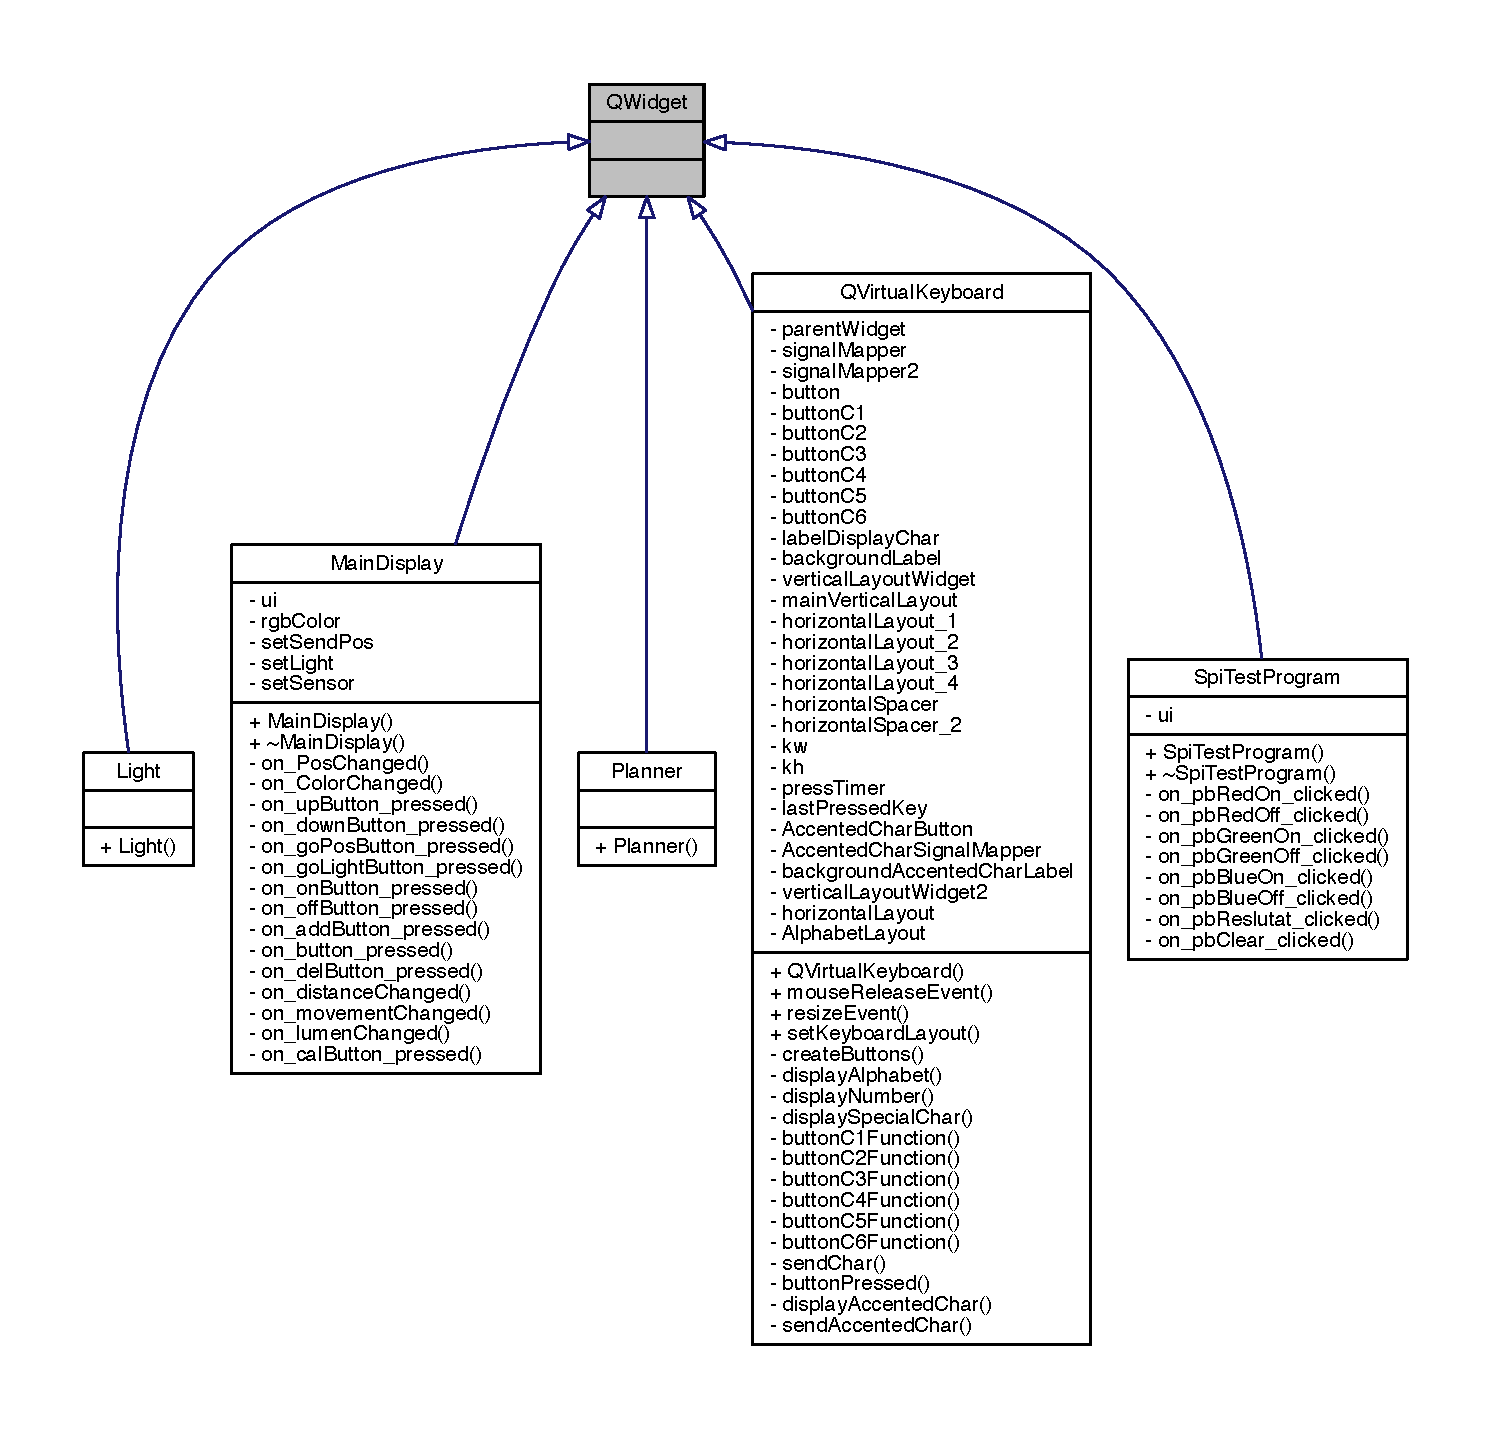
\includegraphics[width=350pt]{de/d92/class_q_widget__inherit__graph}
\end{center}
\end{figure}


Samarbejdsdiagram for Q\+Widget\+:
\nopagebreak
\begin{figure}[H]
\begin{center}
\leavevmode
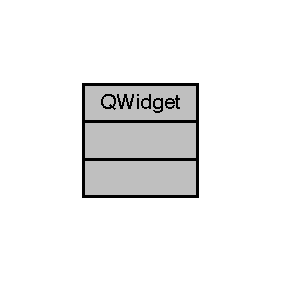
\includegraphics[width=135pt]{d2/d3b/class_q_widget__coll__graph}
\end{center}
\end{figure}


Dokumentationen for denne klasse blev genereret ud fra filen\+:\begin{DoxyCompactItemize}
\item 
\hyperlink{spitestprogram_8h}{spitestprogram.\+h}\end{DoxyCompactItemize}

\hypertarget{class_s_p_iapi}{}\subsection{S\+P\+Iapi Klasse-\/reference}
\label{class_s_p_iapi}\index{S\+P\+Iapi@{S\+P\+Iapi}}


{\ttfamily \#include $<$spiapi.\+h$>$}



Samarbejdsdiagram for S\+P\+Iapi\+:
\nopagebreak
\begin{figure}[H]
\begin{center}
\leavevmode
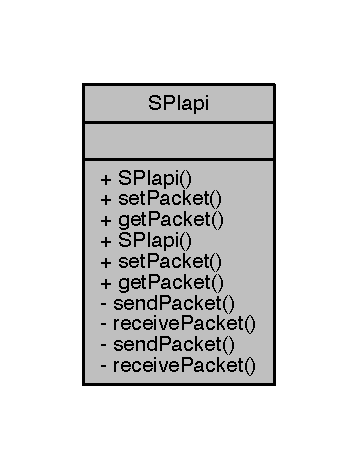
\includegraphics[width=172pt]{dd/d1a/class_s_p_iapi__coll__graph}
\end{center}
\end{figure}
\subsubsection*{Offentlige metoder}
\begin{DoxyCompactItemize}
\item 
\hyperlink{class_s_p_iapi_ae0ce1f581babcf0dab1d0559a352d514}{S\+P\+Iapi} ()
\item 
int \hyperlink{class_s_p_iapi_a197b3f71fa8f68516260bcb3b6985c6b}{set\+Packet} (const unsigned char $\ast$cmd, unsigned char $\ast$value) const 
\item 
int \hyperlink{class_s_p_iapi_afce62b978fa58c0ccefe336835cda0bb}{get\+Packet} (unsigned char $\ast$cmd, unsigned int $\ast$value)
\item 
\hyperlink{class_s_p_iapi_ae0ce1f581babcf0dab1d0559a352d514}{S\+P\+Iapi} ()
\item 
int \hyperlink{class_s_p_iapi_ad5902c2fbc9a0b0a4c807b9da5197fcf}{set\+Packet} (unsigned char $\ast$cmd, unsigned char $\ast$value) const 
\item 
int \hyperlink{class_s_p_iapi_afce62b978fa58c0ccefe336835cda0bb}{get\+Packet} (unsigned char $\ast$cmd, unsigned int $\ast$value)
\end{DoxyCompactItemize}
\subsubsection*{Private metoder}
\begin{DoxyCompactItemize}
\item 
int \hyperlink{class_s_p_iapi_aeeb857d3584d80daa2588a4d971b248e}{send\+Packet} (const unsigned char $\ast$cmd, unsigned char $\ast$data) const 
\item 
int \hyperlink{class_s_p_iapi_a65cbe59b0788556afcfdcac59de1752a}{receive\+Packet} (unsigned char $\ast$cmd, unsigned int $\ast$data)
\item 
int \hyperlink{class_s_p_iapi_a8159ee4c56139354ea1302bb64b99a2d}{send\+Packet} (unsigned char $\ast$cmd, unsigned char $\ast$data) const 
\item 
int \hyperlink{class_s_p_iapi_a65cbe59b0788556afcfdcac59de1752a}{receive\+Packet} (unsigned char $\ast$cmd, unsigned int $\ast$data)
\end{DoxyCompactItemize}


\subsubsection{Detaljeret beskrivelse}
\begin{DoxyAuthor}{Forfatter}
Victor Busk (\href{mailto:201409557@post.au.dk}{\tt 201409557@post.\+au.\+dk}) 
\end{DoxyAuthor}


Defineret på linje 27 i filen Semesterprojekt3/spiapi.\+h.



\subsubsection{Dokumentation af konstruktører og destruktører}
\index{S\+P\+Iapi@{S\+P\+Iapi}!S\+P\+Iapi@{S\+P\+Iapi}}
\index{S\+P\+Iapi@{S\+P\+Iapi}!S\+P\+Iapi@{S\+P\+Iapi}}
\paragraph[{\texorpdfstring{S\+P\+Iapi()}{SPIapi()}}]{\setlength{\rightskip}{0pt plus 5cm}{\bf S\+P\+Iapi} (
\begin{DoxyParamCaption}
{}
\end{DoxyParamCaption}
)}\hypertarget{class_s_p_iapi_ae0ce1f581babcf0dab1d0559a352d514}{}\label{class_s_p_iapi_ae0ce1f581babcf0dab1d0559a352d514}
\index{S\+P\+Iapi@{S\+P\+Iapi}!S\+P\+Iapi@{S\+P\+Iapi}}
\index{S\+P\+Iapi@{S\+P\+Iapi}!S\+P\+Iapi@{S\+P\+Iapi}}
\paragraph[{\texorpdfstring{S\+P\+Iapi()}{SPIapi()}}]{\setlength{\rightskip}{0pt plus 5cm}{\bf S\+P\+Iapi} (
\begin{DoxyParamCaption}
{}
\end{DoxyParamCaption}
)}\hypertarget{class_s_p_iapi_ae0ce1f581babcf0dab1d0559a352d514}{}\label{class_s_p_iapi_ae0ce1f581babcf0dab1d0559a352d514}


\subsubsection{Dokumentation af medlemsfunktioner}
\index{S\+P\+Iapi@{S\+P\+Iapi}!get\+Packet@{get\+Packet}}
\index{get\+Packet@{get\+Packet}!S\+P\+Iapi@{S\+P\+Iapi}}
\paragraph[{\texorpdfstring{get\+Packet(unsigned char $\ast$cmd, unsigned int $\ast$value)}{getPacket(unsigned char *cmd, unsigned int *value)}}]{\setlength{\rightskip}{0pt plus 5cm}int get\+Packet (
\begin{DoxyParamCaption}
\item[{unsigned char $\ast$}]{cmd, }
\item[{unsigned int $\ast$}]{value}
\end{DoxyParamCaption}
)}\hypertarget{class_s_p_iapi_afce62b978fa58c0ccefe336835cda0bb}{}\label{class_s_p_iapi_afce62b978fa58c0ccefe336835cda0bb}
\index{S\+P\+Iapi@{S\+P\+Iapi}!get\+Packet@{get\+Packet}}
\index{get\+Packet@{get\+Packet}!S\+P\+Iapi@{S\+P\+Iapi}}
\paragraph[{\texorpdfstring{get\+Packet(unsigned char $\ast$cmd, unsigned int $\ast$value)}{getPacket(unsigned char *cmd, unsigned int *value)}}]{\setlength{\rightskip}{0pt plus 5cm}int get\+Packet (
\begin{DoxyParamCaption}
\item[{unsigned char $\ast$}]{cmd, }
\item[{unsigned int $\ast$}]{value}
\end{DoxyParamCaption}
)}\hypertarget{class_s_p_iapi_afce62b978fa58c0ccefe336835cda0bb}{}\label{class_s_p_iapi_afce62b978fa58c0ccefe336835cda0bb}
\index{S\+P\+Iapi@{S\+P\+Iapi}!receive\+Packet@{receive\+Packet}}
\index{receive\+Packet@{receive\+Packet}!S\+P\+Iapi@{S\+P\+Iapi}}
\paragraph[{\texorpdfstring{receive\+Packet(unsigned char $\ast$cmd, unsigned int $\ast$data)}{receivePacket(unsigned char *cmd, unsigned int *data)}}]{\setlength{\rightskip}{0pt plus 5cm}int receive\+Packet (
\begin{DoxyParamCaption}
\item[{unsigned char $\ast$}]{cmd, }
\item[{unsigned int $\ast$}]{data}
\end{DoxyParamCaption}
)\hspace{0.3cm}{\ttfamily [private]}}\hypertarget{class_s_p_iapi_a65cbe59b0788556afcfdcac59de1752a}{}\label{class_s_p_iapi_a65cbe59b0788556afcfdcac59de1752a}
\index{S\+P\+Iapi@{S\+P\+Iapi}!receive\+Packet@{receive\+Packet}}
\index{receive\+Packet@{receive\+Packet}!S\+P\+Iapi@{S\+P\+Iapi}}
\paragraph[{\texorpdfstring{receive\+Packet(unsigned char $\ast$cmd, unsigned int $\ast$data)}{receivePacket(unsigned char *cmd, unsigned int *data)}}]{\setlength{\rightskip}{0pt plus 5cm}int receive\+Packet (
\begin{DoxyParamCaption}
\item[{unsigned char $\ast$}]{cmd, }
\item[{unsigned int $\ast$}]{data}
\end{DoxyParamCaption}
)\hspace{0.3cm}{\ttfamily [private]}}\hypertarget{class_s_p_iapi_a65cbe59b0788556afcfdcac59de1752a}{}\label{class_s_p_iapi_a65cbe59b0788556afcfdcac59de1752a}
\index{S\+P\+Iapi@{S\+P\+Iapi}!send\+Packet@{send\+Packet}}
\index{send\+Packet@{send\+Packet}!S\+P\+Iapi@{S\+P\+Iapi}}
\paragraph[{\texorpdfstring{send\+Packet(unsigned char $\ast$cmd, unsigned char $\ast$data) const }{sendPacket(unsigned char *cmd, unsigned char *data) const }}]{\setlength{\rightskip}{0pt plus 5cm}int send\+Packet (
\begin{DoxyParamCaption}
\item[{unsigned char $\ast$}]{cmd, }
\item[{unsigned char $\ast$}]{data}
\end{DoxyParamCaption}
) const\hspace{0.3cm}{\ttfamily [private]}}\hypertarget{class_s_p_iapi_a8159ee4c56139354ea1302bb64b99a2d}{}\label{class_s_p_iapi_a8159ee4c56139354ea1302bb64b99a2d}
\index{S\+P\+Iapi@{S\+P\+Iapi}!send\+Packet@{send\+Packet}}
\index{send\+Packet@{send\+Packet}!S\+P\+Iapi@{S\+P\+Iapi}}
\paragraph[{\texorpdfstring{send\+Packet(const unsigned char $\ast$cmd, unsigned char $\ast$data) const }{sendPacket(const unsigned char *cmd, unsigned char *data) const }}]{\setlength{\rightskip}{0pt plus 5cm}int send\+Packet (
\begin{DoxyParamCaption}
\item[{const unsigned char $\ast$}]{cmd, }
\item[{unsigned char $\ast$}]{data}
\end{DoxyParamCaption}
) const\hspace{0.3cm}{\ttfamily [private]}}\hypertarget{class_s_p_iapi_aeeb857d3584d80daa2588a4d971b248e}{}\label{class_s_p_iapi_aeeb857d3584d80daa2588a4d971b248e}
\index{S\+P\+Iapi@{S\+P\+Iapi}!set\+Packet@{set\+Packet}}
\index{set\+Packet@{set\+Packet}!S\+P\+Iapi@{S\+P\+Iapi}}
\paragraph[{\texorpdfstring{set\+Packet(unsigned char $\ast$cmd, unsigned char $\ast$value) const }{setPacket(unsigned char *cmd, unsigned char *value) const }}]{\setlength{\rightskip}{0pt plus 5cm}int set\+Packet (
\begin{DoxyParamCaption}
\item[{unsigned char $\ast$}]{cmd, }
\item[{unsigned char $\ast$}]{value}
\end{DoxyParamCaption}
) const}\hypertarget{class_s_p_iapi_ad5902c2fbc9a0b0a4c807b9da5197fcf}{}\label{class_s_p_iapi_ad5902c2fbc9a0b0a4c807b9da5197fcf}
\index{S\+P\+Iapi@{S\+P\+Iapi}!set\+Packet@{set\+Packet}}
\index{set\+Packet@{set\+Packet}!S\+P\+Iapi@{S\+P\+Iapi}}
\paragraph[{\texorpdfstring{set\+Packet(const unsigned char $\ast$cmd, unsigned char $\ast$value) const }{setPacket(const unsigned char *cmd, unsigned char *value) const }}]{\setlength{\rightskip}{0pt plus 5cm}int set\+Packet (
\begin{DoxyParamCaption}
\item[{const unsigned char $\ast$}]{cmd, }
\item[{unsigned char $\ast$}]{value}
\end{DoxyParamCaption}
) const}\hypertarget{class_s_p_iapi_a197b3f71fa8f68516260bcb3b6985c6b}{}\label{class_s_p_iapi_a197b3f71fa8f68516260bcb3b6985c6b}


Dokumentationen for denne klasse blev genereret ud fra filen\+:\begin{DoxyCompactItemize}
\item 
\hyperlink{_semesterprojekt3_2spiapi_8h}{Semesterprojekt3/spiapi.\+h}\end{DoxyCompactItemize}

\hypertarget{class_spi_test_program}{}\subsection{Spi\+Test\+Program Klasse-\/reference}
\label{class_spi_test_program}\index{Spi\+Test\+Program@{Spi\+Test\+Program}}


{\ttfamily \#include $<$spitestprogram.\+h$>$}



Stamtræ for Spi\+Test\+Program\+:\nopagebreak
\begin{figure}[H]
\begin{center}
\leavevmode
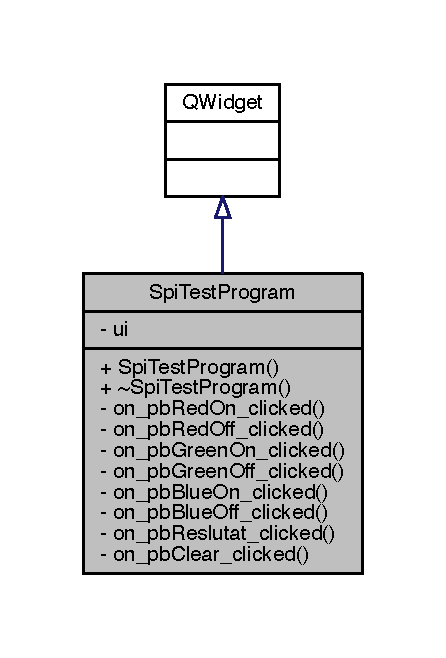
\includegraphics[width=214pt]{dc/d2e/class_spi_test_program__inherit__graph}
\end{center}
\end{figure}


Samarbejdsdiagram for Spi\+Test\+Program\+:\nopagebreak
\begin{figure}[H]
\begin{center}
\leavevmode
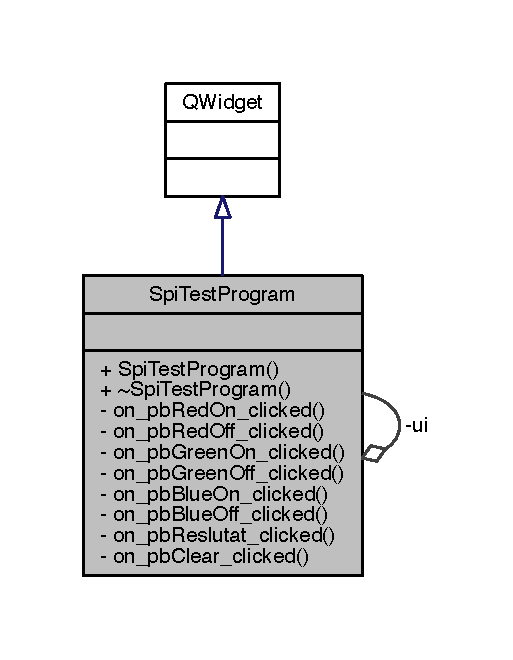
\includegraphics[width=246pt]{d9/d7b/class_spi_test_program__coll__graph}
\end{center}
\end{figure}
\subsubsection*{Offentlige metoder}
\begin{DoxyCompactItemize}
\item 
\hyperlink{class_spi_test_program_aea7280e485f6a12d40676144c83044b7}{Spi\+Test\+Program} (\hyperlink{class_q_widget}{Q\+Widget} $\ast$parent=0)
\item 
\hyperlink{class_spi_test_program_aacfefd1f225cb5dfdade78a4fbee94bd}{$\sim$\+Spi\+Test\+Program} ()
\end{DoxyCompactItemize}
\subsubsection*{Private slots}
\begin{DoxyCompactItemize}
\item 
void \hyperlink{class_spi_test_program_acd8877e279a4f79d7300588b9628bf90}{on\+\_\+pb\+Red\+On\+\_\+clicked} ()
\item 
void \hyperlink{class_spi_test_program_a79cfbfe880f6360ab788d2dc97853d0e}{on\+\_\+pb\+Red\+Off\+\_\+clicked} ()
\item 
void \hyperlink{class_spi_test_program_aa852cac65b64df0aac74a4b95b59a62e}{on\+\_\+pb\+Green\+On\+\_\+clicked} ()
\item 
void \hyperlink{class_spi_test_program_a4b93d87c6f8a6e8eb56f69c0326906af}{on\+\_\+pb\+Green\+Off\+\_\+clicked} ()
\item 
void \hyperlink{class_spi_test_program_ac575e89a52cd7dbeb68a4f5fa4926374}{on\+\_\+pb\+Blue\+On\+\_\+clicked} ()
\item 
void \hyperlink{class_spi_test_program_ada4246a223bc5273c0c53cd993203932}{on\+\_\+pb\+Blue\+Off\+\_\+clicked} ()
\item 
void \hyperlink{class_spi_test_program_acc0c70df85267b31e29c790ca2806895}{on\+\_\+pb\+Reslutat\+\_\+clicked} ()
\item 
void \hyperlink{class_spi_test_program_a5ca1e8292a9ae7b699e6395619650a95}{on\+\_\+pb\+Clear\+\_\+clicked} ()
\end{DoxyCompactItemize}
\subsubsection*{Private attributter}
\begin{DoxyCompactItemize}
\item 
\hyperlink{class_ui_1_1_spi_test_program}{Ui\+::\+Spi\+Test\+Program} $\ast$ \hyperlink{class_spi_test_program_aeb2a16d7ad7ec0f4e767355e60efcf05}{ui}
\end{DoxyCompactItemize}


\subsubsection{Detaljeret beskrivelse}


Defineret på linje 12 i filen spitestprogram.\+h.



\subsubsection{Dokumentation af konstruktører og destruktører}
\index{Spi\+Test\+Program@{Spi\+Test\+Program}!Spi\+Test\+Program@{Spi\+Test\+Program}}
\index{Spi\+Test\+Program@{Spi\+Test\+Program}!Spi\+Test\+Program@{Spi\+Test\+Program}}
\paragraph[{\texorpdfstring{Spi\+Test\+Program(\+Q\+Widget $\ast$parent=0)}{SpiTestProgram(QWidget *parent=0)}}]{\setlength{\rightskip}{0pt plus 5cm}{\bf Spi\+Test\+Program} (
\begin{DoxyParamCaption}
\item[{{\bf Q\+Widget} $\ast$}]{parent = {\ttfamily 0}}
\end{DoxyParamCaption}
)\hspace{0.3cm}{\ttfamily [explicit]}}\hypertarget{class_spi_test_program_aea7280e485f6a12d40676144c83044b7}{}\label{class_spi_test_program_aea7280e485f6a12d40676144c83044b7}
\index{Spi\+Test\+Program@{Spi\+Test\+Program}!````~Spi\+Test\+Program@{$\sim$\+Spi\+Test\+Program}}
\index{````~Spi\+Test\+Program@{$\sim$\+Spi\+Test\+Program}!Spi\+Test\+Program@{Spi\+Test\+Program}}
\paragraph[{\texorpdfstring{$\sim$\+Spi\+Test\+Program()}{~SpiTestProgram()}}]{\setlength{\rightskip}{0pt plus 5cm}$\sim${\bf Spi\+Test\+Program} (
\begin{DoxyParamCaption}
{}
\end{DoxyParamCaption}
)}\hypertarget{class_spi_test_program_aacfefd1f225cb5dfdade78a4fbee94bd}{}\label{class_spi_test_program_aacfefd1f225cb5dfdade78a4fbee94bd}


\subsubsection{Dokumentation af medlemsfunktioner}
\index{Spi\+Test\+Program@{Spi\+Test\+Program}!on\+\_\+pb\+Blue\+Off\+\_\+clicked@{on\+\_\+pb\+Blue\+Off\+\_\+clicked}}
\index{on\+\_\+pb\+Blue\+Off\+\_\+clicked@{on\+\_\+pb\+Blue\+Off\+\_\+clicked}!Spi\+Test\+Program@{Spi\+Test\+Program}}
\paragraph[{\texorpdfstring{on\+\_\+pb\+Blue\+Off\+\_\+clicked}{on_pbBlueOff_clicked}}]{\setlength{\rightskip}{0pt plus 5cm}void on\+\_\+pb\+Blue\+Off\+\_\+clicked (
\begin{DoxyParamCaption}
{}
\end{DoxyParamCaption}
)\hspace{0.3cm}{\ttfamily [private]}, {\ttfamily [slot]}}\hypertarget{class_spi_test_program_ada4246a223bc5273c0c53cd993203932}{}\label{class_spi_test_program_ada4246a223bc5273c0c53cd993203932}
\index{Spi\+Test\+Program@{Spi\+Test\+Program}!on\+\_\+pb\+Blue\+On\+\_\+clicked@{on\+\_\+pb\+Blue\+On\+\_\+clicked}}
\index{on\+\_\+pb\+Blue\+On\+\_\+clicked@{on\+\_\+pb\+Blue\+On\+\_\+clicked}!Spi\+Test\+Program@{Spi\+Test\+Program}}
\paragraph[{\texorpdfstring{on\+\_\+pb\+Blue\+On\+\_\+clicked}{on_pbBlueOn_clicked}}]{\setlength{\rightskip}{0pt plus 5cm}void on\+\_\+pb\+Blue\+On\+\_\+clicked (
\begin{DoxyParamCaption}
{}
\end{DoxyParamCaption}
)\hspace{0.3cm}{\ttfamily [private]}, {\ttfamily [slot]}}\hypertarget{class_spi_test_program_ac575e89a52cd7dbeb68a4f5fa4926374}{}\label{class_spi_test_program_ac575e89a52cd7dbeb68a4f5fa4926374}
\index{Spi\+Test\+Program@{Spi\+Test\+Program}!on\+\_\+pb\+Clear\+\_\+clicked@{on\+\_\+pb\+Clear\+\_\+clicked}}
\index{on\+\_\+pb\+Clear\+\_\+clicked@{on\+\_\+pb\+Clear\+\_\+clicked}!Spi\+Test\+Program@{Spi\+Test\+Program}}
\paragraph[{\texorpdfstring{on\+\_\+pb\+Clear\+\_\+clicked}{on_pbClear_clicked}}]{\setlength{\rightskip}{0pt plus 5cm}void on\+\_\+pb\+Clear\+\_\+clicked (
\begin{DoxyParamCaption}
{}
\end{DoxyParamCaption}
)\hspace{0.3cm}{\ttfamily [private]}, {\ttfamily [slot]}}\hypertarget{class_spi_test_program_a5ca1e8292a9ae7b699e6395619650a95}{}\label{class_spi_test_program_a5ca1e8292a9ae7b699e6395619650a95}
\index{Spi\+Test\+Program@{Spi\+Test\+Program}!on\+\_\+pb\+Green\+Off\+\_\+clicked@{on\+\_\+pb\+Green\+Off\+\_\+clicked}}
\index{on\+\_\+pb\+Green\+Off\+\_\+clicked@{on\+\_\+pb\+Green\+Off\+\_\+clicked}!Spi\+Test\+Program@{Spi\+Test\+Program}}
\paragraph[{\texorpdfstring{on\+\_\+pb\+Green\+Off\+\_\+clicked}{on_pbGreenOff_clicked}}]{\setlength{\rightskip}{0pt plus 5cm}void on\+\_\+pb\+Green\+Off\+\_\+clicked (
\begin{DoxyParamCaption}
{}
\end{DoxyParamCaption}
)\hspace{0.3cm}{\ttfamily [private]}, {\ttfamily [slot]}}\hypertarget{class_spi_test_program_a4b93d87c6f8a6e8eb56f69c0326906af}{}\label{class_spi_test_program_a4b93d87c6f8a6e8eb56f69c0326906af}
\index{Spi\+Test\+Program@{Spi\+Test\+Program}!on\+\_\+pb\+Green\+On\+\_\+clicked@{on\+\_\+pb\+Green\+On\+\_\+clicked}}
\index{on\+\_\+pb\+Green\+On\+\_\+clicked@{on\+\_\+pb\+Green\+On\+\_\+clicked}!Spi\+Test\+Program@{Spi\+Test\+Program}}
\paragraph[{\texorpdfstring{on\+\_\+pb\+Green\+On\+\_\+clicked}{on_pbGreenOn_clicked}}]{\setlength{\rightskip}{0pt plus 5cm}void on\+\_\+pb\+Green\+On\+\_\+clicked (
\begin{DoxyParamCaption}
{}
\end{DoxyParamCaption}
)\hspace{0.3cm}{\ttfamily [private]}, {\ttfamily [slot]}}\hypertarget{class_spi_test_program_aa852cac65b64df0aac74a4b95b59a62e}{}\label{class_spi_test_program_aa852cac65b64df0aac74a4b95b59a62e}
\index{Spi\+Test\+Program@{Spi\+Test\+Program}!on\+\_\+pb\+Red\+Off\+\_\+clicked@{on\+\_\+pb\+Red\+Off\+\_\+clicked}}
\index{on\+\_\+pb\+Red\+Off\+\_\+clicked@{on\+\_\+pb\+Red\+Off\+\_\+clicked}!Spi\+Test\+Program@{Spi\+Test\+Program}}
\paragraph[{\texorpdfstring{on\+\_\+pb\+Red\+Off\+\_\+clicked}{on_pbRedOff_clicked}}]{\setlength{\rightskip}{0pt plus 5cm}void on\+\_\+pb\+Red\+Off\+\_\+clicked (
\begin{DoxyParamCaption}
{}
\end{DoxyParamCaption}
)\hspace{0.3cm}{\ttfamily [private]}, {\ttfamily [slot]}}\hypertarget{class_spi_test_program_a79cfbfe880f6360ab788d2dc97853d0e}{}\label{class_spi_test_program_a79cfbfe880f6360ab788d2dc97853d0e}
\index{Spi\+Test\+Program@{Spi\+Test\+Program}!on\+\_\+pb\+Red\+On\+\_\+clicked@{on\+\_\+pb\+Red\+On\+\_\+clicked}}
\index{on\+\_\+pb\+Red\+On\+\_\+clicked@{on\+\_\+pb\+Red\+On\+\_\+clicked}!Spi\+Test\+Program@{Spi\+Test\+Program}}
\paragraph[{\texorpdfstring{on\+\_\+pb\+Red\+On\+\_\+clicked}{on_pbRedOn_clicked}}]{\setlength{\rightskip}{0pt plus 5cm}void on\+\_\+pb\+Red\+On\+\_\+clicked (
\begin{DoxyParamCaption}
{}
\end{DoxyParamCaption}
)\hspace{0.3cm}{\ttfamily [private]}, {\ttfamily [slot]}}\hypertarget{class_spi_test_program_acd8877e279a4f79d7300588b9628bf90}{}\label{class_spi_test_program_acd8877e279a4f79d7300588b9628bf90}
\index{Spi\+Test\+Program@{Spi\+Test\+Program}!on\+\_\+pb\+Reslutat\+\_\+clicked@{on\+\_\+pb\+Reslutat\+\_\+clicked}}
\index{on\+\_\+pb\+Reslutat\+\_\+clicked@{on\+\_\+pb\+Reslutat\+\_\+clicked}!Spi\+Test\+Program@{Spi\+Test\+Program}}
\paragraph[{\texorpdfstring{on\+\_\+pb\+Reslutat\+\_\+clicked}{on_pbReslutat_clicked}}]{\setlength{\rightskip}{0pt plus 5cm}void on\+\_\+pb\+Reslutat\+\_\+clicked (
\begin{DoxyParamCaption}
{}
\end{DoxyParamCaption}
)\hspace{0.3cm}{\ttfamily [private]}, {\ttfamily [slot]}}\hypertarget{class_spi_test_program_acc0c70df85267b31e29c790ca2806895}{}\label{class_spi_test_program_acc0c70df85267b31e29c790ca2806895}


\subsubsection{Felt-\/dokumentation}
\index{Spi\+Test\+Program@{Spi\+Test\+Program}!ui@{ui}}
\index{ui@{ui}!Spi\+Test\+Program@{Spi\+Test\+Program}}
\paragraph[{\texorpdfstring{ui}{ui}}]{\setlength{\rightskip}{0pt plus 5cm}{\bf Ui\+::\+Spi\+Test\+Program}$\ast$ ui\hspace{0.3cm}{\ttfamily [private]}}\hypertarget{class_spi_test_program_aeb2a16d7ad7ec0f4e767355e60efcf05}{}\label{class_spi_test_program_aeb2a16d7ad7ec0f4e767355e60efcf05}


Defineret på linje 31 i filen spitestprogram.\+h.



Dokumentationen for denne klasse blev genereret ud fra filen\+:\begin{DoxyCompactItemize}
\item 
\hyperlink{spitestprogram_8h}{spitestprogram.\+h}\end{DoxyCompactItemize}

\hypertarget{class_ui_1_1_spi_test_program}{}\subsection{Spi\+Test\+Program Klasse-\/reference}
\label{class_ui_1_1_spi_test_program}\index{Spi\+Test\+Program@{Spi\+Test\+Program}}


{\ttfamily \#include $<$ui\+\_\+spitestprogram.\+h$>$}



Stamtræ for Spi\+Test\+Program\+:\nopagebreak
\begin{figure}[H]
\begin{center}
\leavevmode
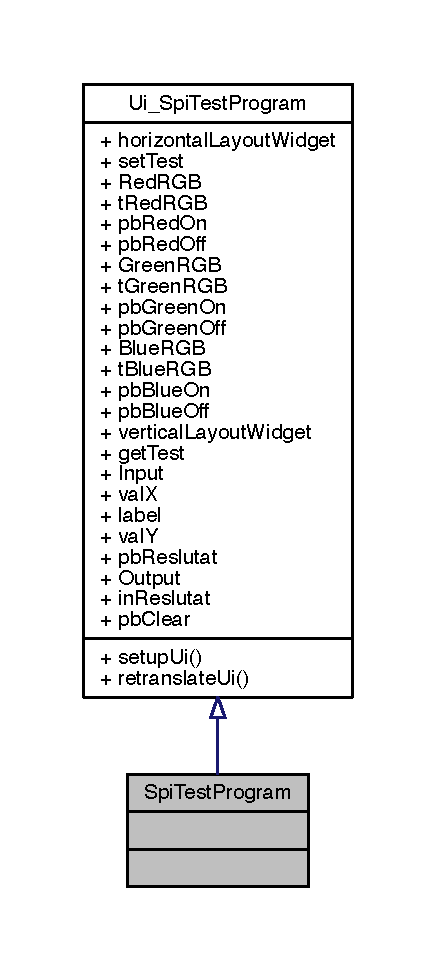
\includegraphics[width=209pt]{d7/d7b/class_ui_1_1_spi_test_program__inherit__graph}
\end{center}
\end{figure}


Samarbejdsdiagram for Spi\+Test\+Program\+:\nopagebreak
\begin{figure}[H]
\begin{center}
\leavevmode
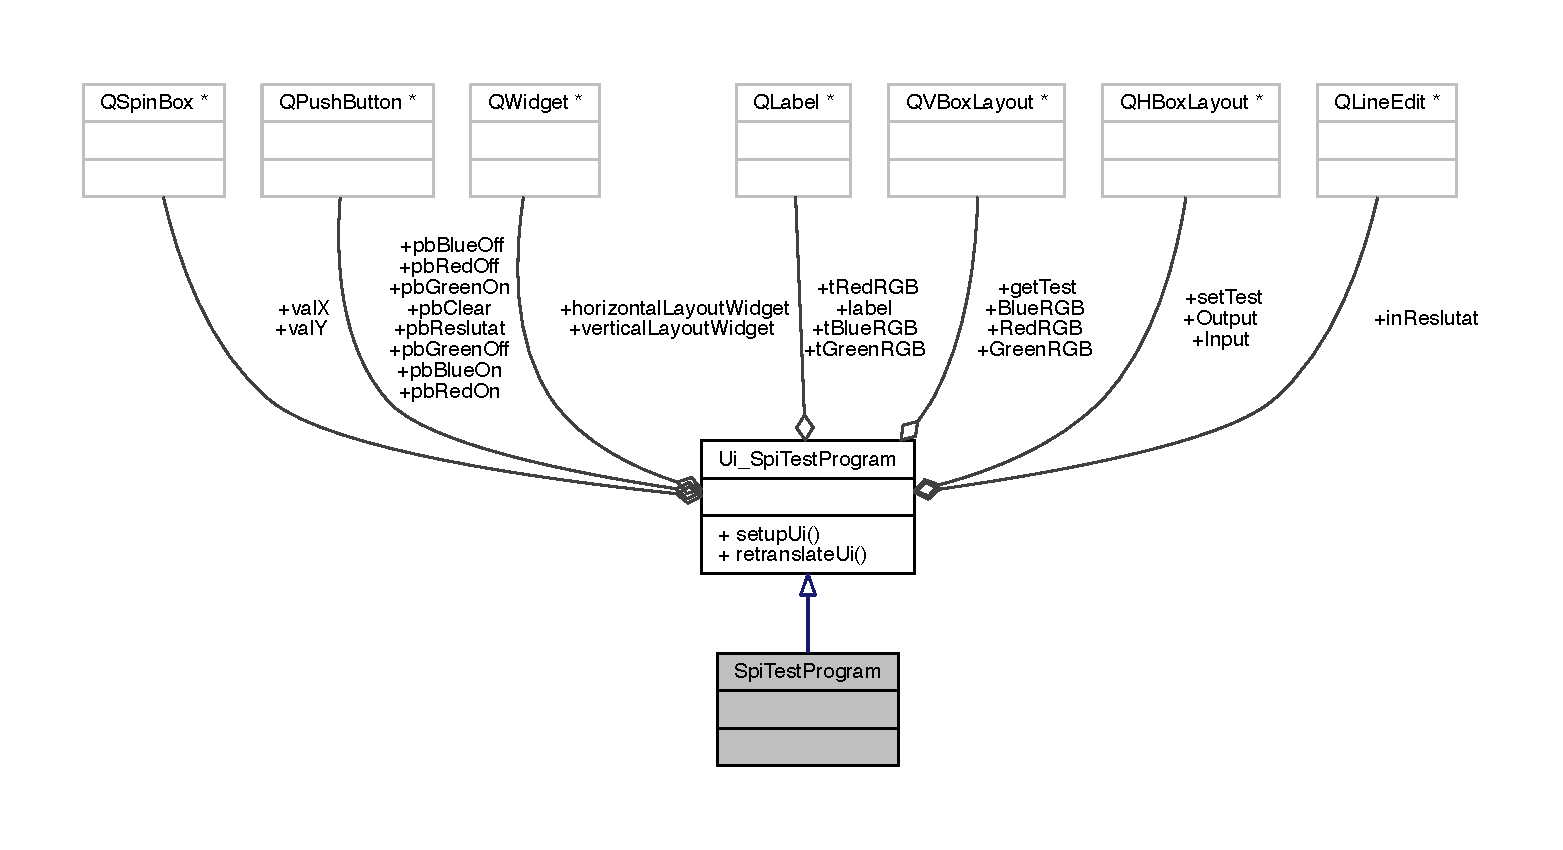
\includegraphics[width=350pt]{d1/d8e/class_ui_1_1_spi_test_program__coll__graph}
\end{center}
\end{figure}
\subsubsection*{Offentlige metoder}
\begin{DoxyCompactItemize}
\item 
void \hyperlink{class_ui___spi_test_program_a6408f1f402f52e12590b3e4968c84e34}{setup\+Ui} (\hyperlink{class_q_widget}{Q\+Widget} $\ast$\hyperlink{class_ui_1_1_spi_test_program}{Spi\+Test\+Program})
\item 
void \hyperlink{class_ui___spi_test_program_a0a1a85fdc36cee52aac338ef3494f996}{retranslate\+Ui} (\hyperlink{class_q_widget}{Q\+Widget} $\ast$\hyperlink{class_ui_1_1_spi_test_program}{Spi\+Test\+Program})
\end{DoxyCompactItemize}
\subsubsection*{Datafelter}
\begin{DoxyCompactItemize}
\item 
\hyperlink{class_q_widget}{Q\+Widget} $\ast$ \hyperlink{class_ui___spi_test_program_a8d9662f61dc85ce78495602f1d03006f}{horizontal\+Layout\+Widget}
\item 
Q\+H\+Box\+Layout $\ast$ \hyperlink{class_ui___spi_test_program_ab40f35f9bcce17af63ba573e1e8ee485}{set\+Test}
\item 
Q\+V\+Box\+Layout $\ast$ \hyperlink{class_ui___spi_test_program_a266d140f4ccd88877aee1b242908b21d}{Red\+R\+GB}
\item 
Q\+Label $\ast$ \hyperlink{class_ui___spi_test_program_a44f9277d36451995887541d6e333c772}{t\+Red\+R\+GB}
\item 
Q\+Push\+Button $\ast$ \hyperlink{class_ui___spi_test_program_a58972344360380ab7a3cedec6de9fb0d}{pb\+Red\+On}
\item 
Q\+Push\+Button $\ast$ \hyperlink{class_ui___spi_test_program_ad6661caed9d7154252ff188ea62e538c}{pb\+Red\+Off}
\item 
Q\+V\+Box\+Layout $\ast$ \hyperlink{class_ui___spi_test_program_a45540b28778c355f4e372566eb065ef3}{Green\+R\+GB}
\item 
Q\+Label $\ast$ \hyperlink{class_ui___spi_test_program_a56e39ae0021a6fba651282c09e6d38da}{t\+Green\+R\+GB}
\item 
Q\+Push\+Button $\ast$ \hyperlink{class_ui___spi_test_program_aa00d405e11fadc9dd8d0b7aae2632903}{pb\+Green\+On}
\item 
Q\+Push\+Button $\ast$ \hyperlink{class_ui___spi_test_program_ad4aa6f2ff845832ee96f6158c85bbfba}{pb\+Green\+Off}
\item 
Q\+V\+Box\+Layout $\ast$ \hyperlink{class_ui___spi_test_program_ac0ff6df3d4236129efdc0762eed715f4}{Blue\+R\+GB}
\item 
Q\+Label $\ast$ \hyperlink{class_ui___spi_test_program_a24f37f517fcdcba9802de32d4cb7cd2a}{t\+Blue\+R\+GB}
\item 
Q\+Push\+Button $\ast$ \hyperlink{class_ui___spi_test_program_a3f13697eb9ebac3370cf5b1456bb2ab6}{pb\+Blue\+On}
\item 
Q\+Push\+Button $\ast$ \hyperlink{class_ui___spi_test_program_add50c8a20a19c966af33418b767fb815}{pb\+Blue\+Off}
\item 
\hyperlink{class_q_widget}{Q\+Widget} $\ast$ \hyperlink{class_ui___spi_test_program_a4dab2ee47678bbea22fe10267a009293}{vertical\+Layout\+Widget}
\item 
Q\+V\+Box\+Layout $\ast$ \hyperlink{class_ui___spi_test_program_a6d63969ee767e7e499a5c6abd4424553}{get\+Test}
\item 
Q\+H\+Box\+Layout $\ast$ \hyperlink{class_ui___spi_test_program_a69c0d851a1ffb0301d02c43531ba2f6d}{Input}
\item 
Q\+Spin\+Box $\ast$ \hyperlink{class_ui___spi_test_program_a54b0fe6bef639246ec21b3109185814a}{valX}
\item 
Q\+Label $\ast$ \hyperlink{class_ui___spi_test_program_a22925632964060df176ccbc0de5fa511}{label}
\item 
Q\+Spin\+Box $\ast$ \hyperlink{class_ui___spi_test_program_a88a3fae2c7f772ec60bc66742e8c097e}{valY}
\item 
Q\+Push\+Button $\ast$ \hyperlink{class_ui___spi_test_program_ac3e098e270e17081064d010d68e7f0fc}{pb\+Reslutat}
\item 
Q\+H\+Box\+Layout $\ast$ \hyperlink{class_ui___spi_test_program_a535084bb7ec3f177d317c38db7e93aa6}{Output}
\item 
Q\+Line\+Edit $\ast$ \hyperlink{class_ui___spi_test_program_a14fdf98633693052d40f7b3dfaa64149}{in\+Reslutat}
\item 
Q\+Push\+Button $\ast$ \hyperlink{class_ui___spi_test_program_a9fa60ac8492007635b4648a0c6c88201}{pb\+Clear}
\end{DoxyCompactItemize}


\subsubsection{Detaljeret beskrivelse}


Defineret på linje 234 i filen ui\+\_\+spitestprogram.\+h.



\subsubsection{Dokumentation af medlemsfunktioner}
\index{Ui\+::\+Spi\+Test\+Program@{Ui\+::\+Spi\+Test\+Program}!retranslate\+Ui@{retranslate\+Ui}}
\index{retranslate\+Ui@{retranslate\+Ui}!Ui\+::\+Spi\+Test\+Program@{Ui\+::\+Spi\+Test\+Program}}
\paragraph[{\texorpdfstring{retranslate\+Ui(\+Q\+Widget $\ast$\+Spi\+Test\+Program)}{retranslateUi(QWidget *SpiTestProgram)}}]{\setlength{\rightskip}{0pt plus 5cm}void retranslate\+Ui (
\begin{DoxyParamCaption}
\item[{{\bf Q\+Widget} $\ast$}]{Spi\+Test\+Program}
\end{DoxyParamCaption}
)\hspace{0.3cm}{\ttfamily [inline]}, {\ttfamily [inherited]}}\hypertarget{class_ui___spi_test_program_a0a1a85fdc36cee52aac338ef3494f996}{}\label{class_ui___spi_test_program_a0a1a85fdc36cee52aac338ef3494f996}


Defineret på linje 214 i filen ui\+\_\+spitestprogram.\+h.



Refereret til af Ui\+\_\+\+Spi\+Test\+Program\+::setup\+Ui().


\begin{DoxyCode}
215     \{
216         \hyperlink{class_ui___spi_test_program_a44f9277d36451995887541d6e333c772}{tRedRGB}->setText(QApplication::translate(\textcolor{stringliteral}{"SpiTestProgram"}, \textcolor{stringliteral}{"Red RGB"}, 0, 
      QApplication::UnicodeUTF8));
217         \hyperlink{class_ui___spi_test_program_a58972344360380ab7a3cedec6de9fb0d}{pbRedOn}->setText(QApplication::translate(\textcolor{stringliteral}{"SpiTestProgram"}, \textcolor{stringliteral}{"On"}, 0, 
      QApplication::UnicodeUTF8));
218         \hyperlink{class_ui___spi_test_program_ad6661caed9d7154252ff188ea62e538c}{pbRedOff}->setText(QApplication::translate(\textcolor{stringliteral}{"SpiTestProgram"}, \textcolor{stringliteral}{"Off"}, 0, 
      QApplication::UnicodeUTF8));
219         \hyperlink{class_ui___spi_test_program_a56e39ae0021a6fba651282c09e6d38da}{tGreenRGB}->setText(QApplication::translate(\textcolor{stringliteral}{"SpiTestProgram"}, \textcolor{stringliteral}{"Green RGB"}, 0, 
      QApplication::UnicodeUTF8));
220         \hyperlink{class_ui___spi_test_program_aa00d405e11fadc9dd8d0b7aae2632903}{pbGreenOn}->setText(QApplication::translate(\textcolor{stringliteral}{"SpiTestProgram"}, \textcolor{stringliteral}{"On"}, 0, 
      QApplication::UnicodeUTF8));
221         \hyperlink{class_ui___spi_test_program_ad4aa6f2ff845832ee96f6158c85bbfba}{pbGreenOff}->setText(QApplication::translate(\textcolor{stringliteral}{"SpiTestProgram"}, \textcolor{stringliteral}{"Off"}, 0, 
      QApplication::UnicodeUTF8));
222         \hyperlink{class_ui___spi_test_program_a24f37f517fcdcba9802de32d4cb7cd2a}{tBlueRGB}->setText(QApplication::translate(\textcolor{stringliteral}{"SpiTestProgram"}, \textcolor{stringliteral}{"Blue RGB"}, 0, 
      QApplication::UnicodeUTF8));
223         \hyperlink{class_ui___spi_test_program_a3f13697eb9ebac3370cf5b1456bb2ab6}{pbBlueOn}->setText(QApplication::translate(\textcolor{stringliteral}{"SpiTestProgram"}, \textcolor{stringliteral}{"On"}, 0, 
      QApplication::UnicodeUTF8));
224         \hyperlink{class_ui___spi_test_program_add50c8a20a19c966af33418b767fb815}{pbBlueOff}->setText(QApplication::translate(\textcolor{stringliteral}{"SpiTestProgram"}, \textcolor{stringliteral}{"Off"}, 0, 
      QApplication::UnicodeUTF8));
225         \hyperlink{class_ui___spi_test_program_a22925632964060df176ccbc0de5fa511}{label}->setText(QApplication::translate(\textcolor{stringliteral}{"SpiTestProgram"}, \textcolor{stringliteral}{"x"}, 0, QApplication::UnicodeUTF8));
226         \hyperlink{class_ui___spi_test_program_ac3e098e270e17081064d010d68e7f0fc}{pbReslutat}->setText(QApplication::translate(\textcolor{stringliteral}{"SpiTestProgram"}, \textcolor{stringliteral}{"Resultat"}, 0, 
      QApplication::UnicodeUTF8));
227         \hyperlink{class_ui___spi_test_program_a9fa60ac8492007635b4648a0c6c88201}{pbClear}->setText(QApplication::translate(\textcolor{stringliteral}{"SpiTestProgram"}, \textcolor{stringliteral}{"Clear"}, 0, 
      QApplication::UnicodeUTF8));
228         Q\_UNUSED(SpiTestProgram);
229     \} \textcolor{comment}{// retranslateUi}
\end{DoxyCode}


Her er kalder-\/grafen for denne funktion\+:\nopagebreak
\begin{figure}[H]
\begin{center}
\leavevmode
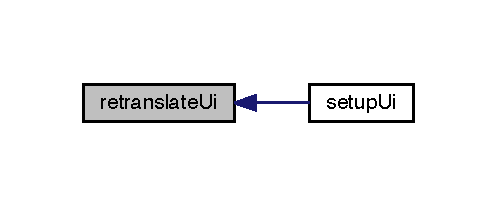
\includegraphics[width=239pt]{d7/de1/class_ui___spi_test_program_a0a1a85fdc36cee52aac338ef3494f996_icgraph}
\end{center}
\end{figure}


\index{Ui\+::\+Spi\+Test\+Program@{Ui\+::\+Spi\+Test\+Program}!setup\+Ui@{setup\+Ui}}
\index{setup\+Ui@{setup\+Ui}!Ui\+::\+Spi\+Test\+Program@{Ui\+::\+Spi\+Test\+Program}}
\paragraph[{\texorpdfstring{setup\+Ui(\+Q\+Widget $\ast$\+Spi\+Test\+Program)}{setupUi(QWidget *SpiTestProgram)}}]{\setlength{\rightskip}{0pt plus 5cm}void setup\+Ui (
\begin{DoxyParamCaption}
\item[{{\bf Q\+Widget} $\ast$}]{Spi\+Test\+Program}
\end{DoxyParamCaption}
)\hspace{0.3cm}{\ttfamily [inline]}, {\ttfamily [inherited]}}\hypertarget{class_ui___spi_test_program_a6408f1f402f52e12590b3e4968c84e34}{}\label{class_ui___spi_test_program_a6408f1f402f52e12590b3e4968c84e34}


Defineret på linje 55 i filen ui\+\_\+spitestprogram.\+h.



Indeholder referencer til Ui\+\_\+\+Spi\+Test\+Program\+::retranslate\+Ui().


\begin{DoxyCode}
56     \{
57         \textcolor{keywordflow}{if} (SpiTestProgram->objectName().isEmpty())
58             SpiTestProgram->setObjectName(QString::fromUtf8(\textcolor{stringliteral}{"SpiTestProgram"}));
59         SpiTestProgram->resize(480, 272);
60         QSizePolicy sizePolicy(QSizePolicy::Fixed, QSizePolicy::Fixed);
61         sizePolicy.setHorizontalStretch(0);
62         sizePolicy.setVerticalStretch(0);
63         sizePolicy.setHeightForWidth(SpiTestProgram->sizePolicy().hasHeightForWidth());
64         SpiTestProgram->setSizePolicy(sizePolicy);
65         SpiTestProgram->setMinimumSize(QSize(480, 272));
66         SpiTestProgram->setMaximumSize(QSize(480, 272));
67         \hyperlink{class_ui___spi_test_program_a8d9662f61dc85ce78495602f1d03006f}{horizontalLayoutWidget} = \textcolor{keyword}{new} \hyperlink{class_q_widget}{QWidget}(SpiTestProgram);
68         \hyperlink{class_ui___spi_test_program_a8d9662f61dc85ce78495602f1d03006f}{horizontalLayoutWidget}->setObjectName(QString::fromUtf8(\textcolor{stringliteral}{"
      horizontalLayoutWidget"}));
69         \hyperlink{class_ui___spi_test_program_a8d9662f61dc85ce78495602f1d03006f}{horizontalLayoutWidget}->setGeometry(QRect(9, 9, 461, 131));
70         \hyperlink{class_ui___spi_test_program_ab40f35f9bcce17af63ba573e1e8ee485}{setTest} = \textcolor{keyword}{new} QHBoxLayout(\hyperlink{class_ui___spi_test_program_a8d9662f61dc85ce78495602f1d03006f}{horizontalLayoutWidget});
71         \hyperlink{class_ui___spi_test_program_ab40f35f9bcce17af63ba573e1e8ee485}{setTest}->setSpacing(6);
72         \hyperlink{class_ui___spi_test_program_ab40f35f9bcce17af63ba573e1e8ee485}{setTest}->setContentsMargins(11, 11, 11, 11);
73         \hyperlink{class_ui___spi_test_program_ab40f35f9bcce17af63ba573e1e8ee485}{setTest}->setObjectName(QString::fromUtf8(\textcolor{stringliteral}{"setTest"}));
74         \hyperlink{class_ui___spi_test_program_ab40f35f9bcce17af63ba573e1e8ee485}{setTest}->setContentsMargins(0, 0, 0, 0);
75         \hyperlink{class_ui___spi_test_program_a266d140f4ccd88877aee1b242908b21d}{RedRGB} = \textcolor{keyword}{new} QVBoxLayout();
76         \hyperlink{class_ui___spi_test_program_a266d140f4ccd88877aee1b242908b21d}{RedRGB}->setSpacing(6);
77         \hyperlink{class_ui___spi_test_program_a266d140f4ccd88877aee1b242908b21d}{RedRGB}->setObjectName(QString::fromUtf8(\textcolor{stringliteral}{"RedRGB"}));
78         \hyperlink{class_ui___spi_test_program_a44f9277d36451995887541d6e333c772}{tRedRGB} = \textcolor{keyword}{new} QLabel(\hyperlink{class_ui___spi_test_program_a8d9662f61dc85ce78495602f1d03006f}{horizontalLayoutWidget});
79         \hyperlink{class_ui___spi_test_program_a44f9277d36451995887541d6e333c772}{tRedRGB}->setObjectName(QString::fromUtf8(\textcolor{stringliteral}{"tRedRGB"}));
80         \hyperlink{class_ui___spi_test_program_a44f9277d36451995887541d6e333c772}{tRedRGB}->setMaximumSize(QSize(272, 30));
81         \hyperlink{class_ui___spi_test_program_a44f9277d36451995887541d6e333c772}{tRedRGB}->setAlignment(Qt::AlignCenter);
82 
83         \hyperlink{class_ui___spi_test_program_a266d140f4ccd88877aee1b242908b21d}{RedRGB}->addWidget(\hyperlink{class_ui___spi_test_program_a44f9277d36451995887541d6e333c772}{tRedRGB});
84 
85         \hyperlink{class_ui___spi_test_program_a58972344360380ab7a3cedec6de9fb0d}{pbRedOn} = \textcolor{keyword}{new} QPushButton(\hyperlink{class_ui___spi_test_program_a8d9662f61dc85ce78495602f1d03006f}{horizontalLayoutWidget});
86         \hyperlink{class_ui___spi_test_program_a58972344360380ab7a3cedec6de9fb0d}{pbRedOn}->setObjectName(QString::fromUtf8(\textcolor{stringliteral}{"pbRedOn"}));
87         \hyperlink{class_ui___spi_test_program_a58972344360380ab7a3cedec6de9fb0d}{pbRedOn}->setMaximumSize(QSize(160, 30));
88 
89         \hyperlink{class_ui___spi_test_program_a266d140f4ccd88877aee1b242908b21d}{RedRGB}->addWidget(\hyperlink{class_ui___spi_test_program_a58972344360380ab7a3cedec6de9fb0d}{pbRedOn});
90 
91         \hyperlink{class_ui___spi_test_program_ad6661caed9d7154252ff188ea62e538c}{pbRedOff} = \textcolor{keyword}{new} QPushButton(\hyperlink{class_ui___spi_test_program_a8d9662f61dc85ce78495602f1d03006f}{horizontalLayoutWidget});
92         \hyperlink{class_ui___spi_test_program_ad6661caed9d7154252ff188ea62e538c}{pbRedOff}->setObjectName(QString::fromUtf8(\textcolor{stringliteral}{"pbRedOff"}));
93         \hyperlink{class_ui___spi_test_program_ad6661caed9d7154252ff188ea62e538c}{pbRedOff}->setMaximumSize(QSize(160, 30));
94 
95         \hyperlink{class_ui___spi_test_program_a266d140f4ccd88877aee1b242908b21d}{RedRGB}->addWidget(\hyperlink{class_ui___spi_test_program_ad6661caed9d7154252ff188ea62e538c}{pbRedOff});
96 
97 
98         \hyperlink{class_ui___spi_test_program_ab40f35f9bcce17af63ba573e1e8ee485}{setTest}->addLayout(\hyperlink{class_ui___spi_test_program_a266d140f4ccd88877aee1b242908b21d}{RedRGB});
99 
100         \hyperlink{class_ui___spi_test_program_a45540b28778c355f4e372566eb065ef3}{GreenRGB} = \textcolor{keyword}{new} QVBoxLayout();
101         \hyperlink{class_ui___spi_test_program_a45540b28778c355f4e372566eb065ef3}{GreenRGB}->setSpacing(6);
102         \hyperlink{class_ui___spi_test_program_a45540b28778c355f4e372566eb065ef3}{GreenRGB}->setObjectName(QString::fromUtf8(\textcolor{stringliteral}{"GreenRGB"}));
103         \hyperlink{class_ui___spi_test_program_a56e39ae0021a6fba651282c09e6d38da}{tGreenRGB} = \textcolor{keyword}{new} QLabel(\hyperlink{class_ui___spi_test_program_a8d9662f61dc85ce78495602f1d03006f}{horizontalLayoutWidget});
104         \hyperlink{class_ui___spi_test_program_a56e39ae0021a6fba651282c09e6d38da}{tGreenRGB}->setObjectName(QString::fromUtf8(\textcolor{stringliteral}{"tGreenRGB"}));
105         \hyperlink{class_ui___spi_test_program_a56e39ae0021a6fba651282c09e6d38da}{tGreenRGB}->setMaximumSize(QSize(160, 30));
106         \hyperlink{class_ui___spi_test_program_a56e39ae0021a6fba651282c09e6d38da}{tGreenRGB}->setAlignment(Qt::AlignCenter);
107 
108         \hyperlink{class_ui___spi_test_program_a45540b28778c355f4e372566eb065ef3}{GreenRGB}->addWidget(\hyperlink{class_ui___spi_test_program_a56e39ae0021a6fba651282c09e6d38da}{tGreenRGB});
109 
110         \hyperlink{class_ui___spi_test_program_aa00d405e11fadc9dd8d0b7aae2632903}{pbGreenOn} = \textcolor{keyword}{new} QPushButton(\hyperlink{class_ui___spi_test_program_a8d9662f61dc85ce78495602f1d03006f}{horizontalLayoutWidget});
111         \hyperlink{class_ui___spi_test_program_aa00d405e11fadc9dd8d0b7aae2632903}{pbGreenOn}->setObjectName(QString::fromUtf8(\textcolor{stringliteral}{"pbGreenOn"}));
112         \hyperlink{class_ui___spi_test_program_aa00d405e11fadc9dd8d0b7aae2632903}{pbGreenOn}->setMaximumSize(QSize(160, 30));
113 
114         \hyperlink{class_ui___spi_test_program_a45540b28778c355f4e372566eb065ef3}{GreenRGB}->addWidget(\hyperlink{class_ui___spi_test_program_aa00d405e11fadc9dd8d0b7aae2632903}{pbGreenOn});
115 
116         \hyperlink{class_ui___spi_test_program_ad4aa6f2ff845832ee96f6158c85bbfba}{pbGreenOff} = \textcolor{keyword}{new} QPushButton(\hyperlink{class_ui___spi_test_program_a8d9662f61dc85ce78495602f1d03006f}{horizontalLayoutWidget});
117         \hyperlink{class_ui___spi_test_program_ad4aa6f2ff845832ee96f6158c85bbfba}{pbGreenOff}->setObjectName(QString::fromUtf8(\textcolor{stringliteral}{"pbGreenOff"}));
118         \hyperlink{class_ui___spi_test_program_ad4aa6f2ff845832ee96f6158c85bbfba}{pbGreenOff}->setMaximumSize(QSize(160, 30));
119 
120         \hyperlink{class_ui___spi_test_program_a45540b28778c355f4e372566eb065ef3}{GreenRGB}->addWidget(\hyperlink{class_ui___spi_test_program_ad4aa6f2ff845832ee96f6158c85bbfba}{pbGreenOff});
121 
122 
123         \hyperlink{class_ui___spi_test_program_ab40f35f9bcce17af63ba573e1e8ee485}{setTest}->addLayout(\hyperlink{class_ui___spi_test_program_a45540b28778c355f4e372566eb065ef3}{GreenRGB});
124 
125         \hyperlink{class_ui___spi_test_program_ac0ff6df3d4236129efdc0762eed715f4}{BlueRGB} = \textcolor{keyword}{new} QVBoxLayout();
126         \hyperlink{class_ui___spi_test_program_ac0ff6df3d4236129efdc0762eed715f4}{BlueRGB}->setSpacing(6);
127         \hyperlink{class_ui___spi_test_program_ac0ff6df3d4236129efdc0762eed715f4}{BlueRGB}->setObjectName(QString::fromUtf8(\textcolor{stringliteral}{"BlueRGB"}));
128         \hyperlink{class_ui___spi_test_program_a24f37f517fcdcba9802de32d4cb7cd2a}{tBlueRGB} = \textcolor{keyword}{new} QLabel(\hyperlink{class_ui___spi_test_program_a8d9662f61dc85ce78495602f1d03006f}{horizontalLayoutWidget});
129         \hyperlink{class_ui___spi_test_program_a24f37f517fcdcba9802de32d4cb7cd2a}{tBlueRGB}->setObjectName(QString::fromUtf8(\textcolor{stringliteral}{"tBlueRGB"}));
130         \hyperlink{class_ui___spi_test_program_a24f37f517fcdcba9802de32d4cb7cd2a}{tBlueRGB}->setMaximumSize(QSize(160, 30));
131         \hyperlink{class_ui___spi_test_program_a24f37f517fcdcba9802de32d4cb7cd2a}{tBlueRGB}->setAlignment(Qt::AlignCenter);
132 
133         \hyperlink{class_ui___spi_test_program_ac0ff6df3d4236129efdc0762eed715f4}{BlueRGB}->addWidget(\hyperlink{class_ui___spi_test_program_a24f37f517fcdcba9802de32d4cb7cd2a}{tBlueRGB});
134 
135         \hyperlink{class_ui___spi_test_program_a3f13697eb9ebac3370cf5b1456bb2ab6}{pbBlueOn} = \textcolor{keyword}{new} QPushButton(\hyperlink{class_ui___spi_test_program_a8d9662f61dc85ce78495602f1d03006f}{horizontalLayoutWidget});
136         \hyperlink{class_ui___spi_test_program_a3f13697eb9ebac3370cf5b1456bb2ab6}{pbBlueOn}->setObjectName(QString::fromUtf8(\textcolor{stringliteral}{"pbBlueOn"}));
137         \hyperlink{class_ui___spi_test_program_a3f13697eb9ebac3370cf5b1456bb2ab6}{pbBlueOn}->setMaximumSize(QSize(160, 30));
138 
139         \hyperlink{class_ui___spi_test_program_ac0ff6df3d4236129efdc0762eed715f4}{BlueRGB}->addWidget(\hyperlink{class_ui___spi_test_program_a3f13697eb9ebac3370cf5b1456bb2ab6}{pbBlueOn});
140 
141         \hyperlink{class_ui___spi_test_program_add50c8a20a19c966af33418b767fb815}{pbBlueOff} = \textcolor{keyword}{new} QPushButton(\hyperlink{class_ui___spi_test_program_a8d9662f61dc85ce78495602f1d03006f}{horizontalLayoutWidget});
142         \hyperlink{class_ui___spi_test_program_add50c8a20a19c966af33418b767fb815}{pbBlueOff}->setObjectName(QString::fromUtf8(\textcolor{stringliteral}{"pbBlueOff"}));
143         \hyperlink{class_ui___spi_test_program_add50c8a20a19c966af33418b767fb815}{pbBlueOff}->setMaximumSize(QSize(160, 30));
144 
145         \hyperlink{class_ui___spi_test_program_ac0ff6df3d4236129efdc0762eed715f4}{BlueRGB}->addWidget(\hyperlink{class_ui___spi_test_program_add50c8a20a19c966af33418b767fb815}{pbBlueOff});
146 
147 
148         \hyperlink{class_ui___spi_test_program_ab40f35f9bcce17af63ba573e1e8ee485}{setTest}->addLayout(\hyperlink{class_ui___spi_test_program_ac0ff6df3d4236129efdc0762eed715f4}{BlueRGB});
149 
150         \hyperlink{class_ui___spi_test_program_a4dab2ee47678bbea22fe10267a009293}{verticalLayoutWidget} = \textcolor{keyword}{new} \hyperlink{class_q_widget}{QWidget}(SpiTestProgram);
151         \hyperlink{class_ui___spi_test_program_a4dab2ee47678bbea22fe10267a009293}{verticalLayoutWidget}->setObjectName(QString::fromUtf8(\textcolor{stringliteral}{"verticalLayoutWidget"}));
152         \hyperlink{class_ui___spi_test_program_a4dab2ee47678bbea22fe10267a009293}{verticalLayoutWidget}->setGeometry(QRect(10, 150, 461, 111));
153         \hyperlink{class_ui___spi_test_program_a6d63969ee767e7e499a5c6abd4424553}{getTest} = \textcolor{keyword}{new} QVBoxLayout(\hyperlink{class_ui___spi_test_program_a4dab2ee47678bbea22fe10267a009293}{verticalLayoutWidget});
154         \hyperlink{class_ui___spi_test_program_a6d63969ee767e7e499a5c6abd4424553}{getTest}->setSpacing(6);
155         \hyperlink{class_ui___spi_test_program_a6d63969ee767e7e499a5c6abd4424553}{getTest}->setContentsMargins(11, 11, 11, 11);
156         \hyperlink{class_ui___spi_test_program_a6d63969ee767e7e499a5c6abd4424553}{getTest}->setObjectName(QString::fromUtf8(\textcolor{stringliteral}{"getTest"}));
157         \hyperlink{class_ui___spi_test_program_a6d63969ee767e7e499a5c6abd4424553}{getTest}->setContentsMargins(0, 0, 0, 0);
158         \hyperlink{class_ui___spi_test_program_a69c0d851a1ffb0301d02c43531ba2f6d}{Input} = \textcolor{keyword}{new} QHBoxLayout();
159         \hyperlink{class_ui___spi_test_program_a69c0d851a1ffb0301d02c43531ba2f6d}{Input}->setSpacing(6);
160         \hyperlink{class_ui___spi_test_program_a69c0d851a1ffb0301d02c43531ba2f6d}{Input}->setObjectName(QString::fromUtf8(\textcolor{stringliteral}{"Input"}));
161         \hyperlink{class_ui___spi_test_program_a54b0fe6bef639246ec21b3109185814a}{valX} = \textcolor{keyword}{new} QSpinBox(\hyperlink{class_ui___spi_test_program_a4dab2ee47678bbea22fe10267a009293}{verticalLayoutWidget});
162         \hyperlink{class_ui___spi_test_program_a54b0fe6bef639246ec21b3109185814a}{valX}->setObjectName(QString::fromUtf8(\textcolor{stringliteral}{"valX"}));
163         \hyperlink{class_ui___spi_test_program_a54b0fe6bef639246ec21b3109185814a}{valX}->setMaximumSize(QSize(160, 30));
164 
165         \hyperlink{class_ui___spi_test_program_a69c0d851a1ffb0301d02c43531ba2f6d}{Input}->addWidget(\hyperlink{class_ui___spi_test_program_a54b0fe6bef639246ec21b3109185814a}{valX});
166 
167         \hyperlink{class_ui___spi_test_program_a22925632964060df176ccbc0de5fa511}{label} = \textcolor{keyword}{new} QLabel(\hyperlink{class_ui___spi_test_program_a4dab2ee47678bbea22fe10267a009293}{verticalLayoutWidget});
168         \hyperlink{class_ui___spi_test_program_a22925632964060df176ccbc0de5fa511}{label}->setObjectName(QString::fromUtf8(\textcolor{stringliteral}{"label"}));
169         \hyperlink{class_ui___spi_test_program_a22925632964060df176ccbc0de5fa511}{label}->setMaximumSize(QSize(20, 30));
170         \hyperlink{class_ui___spi_test_program_a22925632964060df176ccbc0de5fa511}{label}->setAlignment(Qt::AlignCenter);
171 
172         \hyperlink{class_ui___spi_test_program_a69c0d851a1ffb0301d02c43531ba2f6d}{Input}->addWidget(\hyperlink{class_ui___spi_test_program_a22925632964060df176ccbc0de5fa511}{label});
173 
174         \hyperlink{class_ui___spi_test_program_a88a3fae2c7f772ec60bc66742e8c097e}{valY} = \textcolor{keyword}{new} QSpinBox(\hyperlink{class_ui___spi_test_program_a4dab2ee47678bbea22fe10267a009293}{verticalLayoutWidget});
175         \hyperlink{class_ui___spi_test_program_a88a3fae2c7f772ec60bc66742e8c097e}{valY}->setObjectName(QString::fromUtf8(\textcolor{stringliteral}{"valY"}));
176         \hyperlink{class_ui___spi_test_program_a88a3fae2c7f772ec60bc66742e8c097e}{valY}->setMaximumSize(QSize(160, 30));
177 
178         \hyperlink{class_ui___spi_test_program_a69c0d851a1ffb0301d02c43531ba2f6d}{Input}->addWidget(\hyperlink{class_ui___spi_test_program_a88a3fae2c7f772ec60bc66742e8c097e}{valY});
179 
180         \hyperlink{class_ui___spi_test_program_ac3e098e270e17081064d010d68e7f0fc}{pbReslutat} = \textcolor{keyword}{new} QPushButton(\hyperlink{class_ui___spi_test_program_a4dab2ee47678bbea22fe10267a009293}{verticalLayoutWidget});
181         \hyperlink{class_ui___spi_test_program_ac3e098e270e17081064d010d68e7f0fc}{pbReslutat}->setObjectName(QString::fromUtf8(\textcolor{stringliteral}{"pbReslutat"}));
182         \hyperlink{class_ui___spi_test_program_ac3e098e270e17081064d010d68e7f0fc}{pbReslutat}->setMaximumSize(QSize(160, 30));
183 
184         \hyperlink{class_ui___spi_test_program_a69c0d851a1ffb0301d02c43531ba2f6d}{Input}->addWidget(\hyperlink{class_ui___spi_test_program_ac3e098e270e17081064d010d68e7f0fc}{pbReslutat});
185 
186 
187         \hyperlink{class_ui___spi_test_program_a6d63969ee767e7e499a5c6abd4424553}{getTest}->addLayout(\hyperlink{class_ui___spi_test_program_a69c0d851a1ffb0301d02c43531ba2f6d}{Input});
188 
189         \hyperlink{class_ui___spi_test_program_a535084bb7ec3f177d317c38db7e93aa6}{Output} = \textcolor{keyword}{new} QHBoxLayout();
190         \hyperlink{class_ui___spi_test_program_a535084bb7ec3f177d317c38db7e93aa6}{Output}->setSpacing(6);
191         \hyperlink{class_ui___spi_test_program_a535084bb7ec3f177d317c38db7e93aa6}{Output}->setObjectName(QString::fromUtf8(\textcolor{stringliteral}{"Output"}));
192         \hyperlink{class_ui___spi_test_program_a14fdf98633693052d40f7b3dfaa64149}{inReslutat} = \textcolor{keyword}{new} QLineEdit(\hyperlink{class_ui___spi_test_program_a4dab2ee47678bbea22fe10267a009293}{verticalLayoutWidget});
193         \hyperlink{class_ui___spi_test_program_a14fdf98633693052d40f7b3dfaa64149}{inReslutat}->setObjectName(QString::fromUtf8(\textcolor{stringliteral}{"inReslutat"}));
194         \hyperlink{class_ui___spi_test_program_a14fdf98633693052d40f7b3dfaa64149}{inReslutat}->setMaximumSize(QSize(340, 30));
195         \hyperlink{class_ui___spi_test_program_a14fdf98633693052d40f7b3dfaa64149}{inReslutat}->setAlignment(Qt::AlignCenter);
196 
197         \hyperlink{class_ui___spi_test_program_a535084bb7ec3f177d317c38db7e93aa6}{Output}->addWidget(\hyperlink{class_ui___spi_test_program_a14fdf98633693052d40f7b3dfaa64149}{inReslutat});
198 
199         \hyperlink{class_ui___spi_test_program_a9fa60ac8492007635b4648a0c6c88201}{pbClear} = \textcolor{keyword}{new} QPushButton(\hyperlink{class_ui___spi_test_program_a4dab2ee47678bbea22fe10267a009293}{verticalLayoutWidget});
200         \hyperlink{class_ui___spi_test_program_a9fa60ac8492007635b4648a0c6c88201}{pbClear}->setObjectName(QString::fromUtf8(\textcolor{stringliteral}{"pbClear"}));
201         \hyperlink{class_ui___spi_test_program_a9fa60ac8492007635b4648a0c6c88201}{pbClear}->setMaximumSize(QSize(160, 30));
202 
203         \hyperlink{class_ui___spi_test_program_a535084bb7ec3f177d317c38db7e93aa6}{Output}->addWidget(\hyperlink{class_ui___spi_test_program_a9fa60ac8492007635b4648a0c6c88201}{pbClear});
204 
205 
206         \hyperlink{class_ui___spi_test_program_a6d63969ee767e7e499a5c6abd4424553}{getTest}->addLayout(\hyperlink{class_ui___spi_test_program_a535084bb7ec3f177d317c38db7e93aa6}{Output});
207 
208 
209         \hyperlink{class_ui___spi_test_program_a0a1a85fdc36cee52aac338ef3494f996}{retranslateUi}(SpiTestProgram);
210 
211         QMetaObject::connectSlotsByName(SpiTestProgram);
212     \} \textcolor{comment}{// setupUi}
\end{DoxyCode}


Her er kald-\/grafen for denne funktion\+:\nopagebreak
\begin{figure}[H]
\begin{center}
\leavevmode
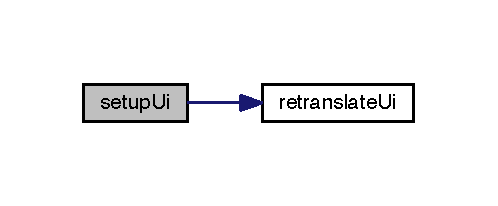
\includegraphics[width=239pt]{d7/de1/class_ui___spi_test_program_a6408f1f402f52e12590b3e4968c84e34_cgraph}
\end{center}
\end{figure}




\subsubsection{Felt-\/dokumentation}
\index{Ui\+::\+Spi\+Test\+Program@{Ui\+::\+Spi\+Test\+Program}!Blue\+R\+GB@{Blue\+R\+GB}}
\index{Blue\+R\+GB@{Blue\+R\+GB}!Ui\+::\+Spi\+Test\+Program@{Ui\+::\+Spi\+Test\+Program}}
\paragraph[{\texorpdfstring{Blue\+R\+GB}{BlueRGB}}]{\setlength{\rightskip}{0pt plus 5cm}Q\+V\+Box\+Layout$\ast$ Blue\+R\+GB\hspace{0.3cm}{\ttfamily [inherited]}}\hypertarget{class_ui___spi_test_program_ac0ff6df3d4236129efdc0762eed715f4}{}\label{class_ui___spi_test_program_ac0ff6df3d4236129efdc0762eed715f4}


Defineret på linje 40 i filen ui\+\_\+spitestprogram.\+h.

\index{Ui\+::\+Spi\+Test\+Program@{Ui\+::\+Spi\+Test\+Program}!get\+Test@{get\+Test}}
\index{get\+Test@{get\+Test}!Ui\+::\+Spi\+Test\+Program@{Ui\+::\+Spi\+Test\+Program}}
\paragraph[{\texorpdfstring{get\+Test}{getTest}}]{\setlength{\rightskip}{0pt plus 5cm}Q\+V\+Box\+Layout$\ast$ get\+Test\hspace{0.3cm}{\ttfamily [inherited]}}\hypertarget{class_ui___spi_test_program_a6d63969ee767e7e499a5c6abd4424553}{}\label{class_ui___spi_test_program_a6d63969ee767e7e499a5c6abd4424553}


Defineret på linje 45 i filen ui\+\_\+spitestprogram.\+h.

\index{Ui\+::\+Spi\+Test\+Program@{Ui\+::\+Spi\+Test\+Program}!Green\+R\+GB@{Green\+R\+GB}}
\index{Green\+R\+GB@{Green\+R\+GB}!Ui\+::\+Spi\+Test\+Program@{Ui\+::\+Spi\+Test\+Program}}
\paragraph[{\texorpdfstring{Green\+R\+GB}{GreenRGB}}]{\setlength{\rightskip}{0pt plus 5cm}Q\+V\+Box\+Layout$\ast$ Green\+R\+GB\hspace{0.3cm}{\ttfamily [inherited]}}\hypertarget{class_ui___spi_test_program_a45540b28778c355f4e372566eb065ef3}{}\label{class_ui___spi_test_program_a45540b28778c355f4e372566eb065ef3}


Defineret på linje 36 i filen ui\+\_\+spitestprogram.\+h.

\index{Ui\+::\+Spi\+Test\+Program@{Ui\+::\+Spi\+Test\+Program}!horizontal\+Layout\+Widget@{horizontal\+Layout\+Widget}}
\index{horizontal\+Layout\+Widget@{horizontal\+Layout\+Widget}!Ui\+::\+Spi\+Test\+Program@{Ui\+::\+Spi\+Test\+Program}}
\paragraph[{\texorpdfstring{horizontal\+Layout\+Widget}{horizontalLayoutWidget}}]{\setlength{\rightskip}{0pt plus 5cm}{\bf Q\+Widget}$\ast$ horizontal\+Layout\+Widget\hspace{0.3cm}{\ttfamily [inherited]}}\hypertarget{class_ui___spi_test_program_a8d9662f61dc85ce78495602f1d03006f}{}\label{class_ui___spi_test_program_a8d9662f61dc85ce78495602f1d03006f}


Defineret på linje 30 i filen ui\+\_\+spitestprogram.\+h.

\index{Ui\+::\+Spi\+Test\+Program@{Ui\+::\+Spi\+Test\+Program}!Input@{Input}}
\index{Input@{Input}!Ui\+::\+Spi\+Test\+Program@{Ui\+::\+Spi\+Test\+Program}}
\paragraph[{\texorpdfstring{Input}{Input}}]{\setlength{\rightskip}{0pt plus 5cm}Q\+H\+Box\+Layout$\ast$ Input\hspace{0.3cm}{\ttfamily [inherited]}}\hypertarget{class_ui___spi_test_program_a69c0d851a1ffb0301d02c43531ba2f6d}{}\label{class_ui___spi_test_program_a69c0d851a1ffb0301d02c43531ba2f6d}


Defineret på linje 46 i filen ui\+\_\+spitestprogram.\+h.

\index{Ui\+::\+Spi\+Test\+Program@{Ui\+::\+Spi\+Test\+Program}!in\+Reslutat@{in\+Reslutat}}
\index{in\+Reslutat@{in\+Reslutat}!Ui\+::\+Spi\+Test\+Program@{Ui\+::\+Spi\+Test\+Program}}
\paragraph[{\texorpdfstring{in\+Reslutat}{inReslutat}}]{\setlength{\rightskip}{0pt plus 5cm}Q\+Line\+Edit$\ast$ in\+Reslutat\hspace{0.3cm}{\ttfamily [inherited]}}\hypertarget{class_ui___spi_test_program_a14fdf98633693052d40f7b3dfaa64149}{}\label{class_ui___spi_test_program_a14fdf98633693052d40f7b3dfaa64149}


Defineret på linje 52 i filen ui\+\_\+spitestprogram.\+h.

\index{Ui\+::\+Spi\+Test\+Program@{Ui\+::\+Spi\+Test\+Program}!label@{label}}
\index{label@{label}!Ui\+::\+Spi\+Test\+Program@{Ui\+::\+Spi\+Test\+Program}}
\paragraph[{\texorpdfstring{label}{label}}]{\setlength{\rightskip}{0pt plus 5cm}Q\+Label$\ast$ label\hspace{0.3cm}{\ttfamily [inherited]}}\hypertarget{class_ui___spi_test_program_a22925632964060df176ccbc0de5fa511}{}\label{class_ui___spi_test_program_a22925632964060df176ccbc0de5fa511}


Defineret på linje 48 i filen ui\+\_\+spitestprogram.\+h.

\index{Ui\+::\+Spi\+Test\+Program@{Ui\+::\+Spi\+Test\+Program}!Output@{Output}}
\index{Output@{Output}!Ui\+::\+Spi\+Test\+Program@{Ui\+::\+Spi\+Test\+Program}}
\paragraph[{\texorpdfstring{Output}{Output}}]{\setlength{\rightskip}{0pt plus 5cm}Q\+H\+Box\+Layout$\ast$ Output\hspace{0.3cm}{\ttfamily [inherited]}}\hypertarget{class_ui___spi_test_program_a535084bb7ec3f177d317c38db7e93aa6}{}\label{class_ui___spi_test_program_a535084bb7ec3f177d317c38db7e93aa6}


Defineret på linje 51 i filen ui\+\_\+spitestprogram.\+h.

\index{Ui\+::\+Spi\+Test\+Program@{Ui\+::\+Spi\+Test\+Program}!pb\+Blue\+Off@{pb\+Blue\+Off}}
\index{pb\+Blue\+Off@{pb\+Blue\+Off}!Ui\+::\+Spi\+Test\+Program@{Ui\+::\+Spi\+Test\+Program}}
\paragraph[{\texorpdfstring{pb\+Blue\+Off}{pbBlueOff}}]{\setlength{\rightskip}{0pt plus 5cm}Q\+Push\+Button$\ast$ pb\+Blue\+Off\hspace{0.3cm}{\ttfamily [inherited]}}\hypertarget{class_ui___spi_test_program_add50c8a20a19c966af33418b767fb815}{}\label{class_ui___spi_test_program_add50c8a20a19c966af33418b767fb815}


Defineret på linje 43 i filen ui\+\_\+spitestprogram.\+h.

\index{Ui\+::\+Spi\+Test\+Program@{Ui\+::\+Spi\+Test\+Program}!pb\+Blue\+On@{pb\+Blue\+On}}
\index{pb\+Blue\+On@{pb\+Blue\+On}!Ui\+::\+Spi\+Test\+Program@{Ui\+::\+Spi\+Test\+Program}}
\paragraph[{\texorpdfstring{pb\+Blue\+On}{pbBlueOn}}]{\setlength{\rightskip}{0pt plus 5cm}Q\+Push\+Button$\ast$ pb\+Blue\+On\hspace{0.3cm}{\ttfamily [inherited]}}\hypertarget{class_ui___spi_test_program_a3f13697eb9ebac3370cf5b1456bb2ab6}{}\label{class_ui___spi_test_program_a3f13697eb9ebac3370cf5b1456bb2ab6}


Defineret på linje 42 i filen ui\+\_\+spitestprogram.\+h.

\index{Ui\+::\+Spi\+Test\+Program@{Ui\+::\+Spi\+Test\+Program}!pb\+Clear@{pb\+Clear}}
\index{pb\+Clear@{pb\+Clear}!Ui\+::\+Spi\+Test\+Program@{Ui\+::\+Spi\+Test\+Program}}
\paragraph[{\texorpdfstring{pb\+Clear}{pbClear}}]{\setlength{\rightskip}{0pt plus 5cm}Q\+Push\+Button$\ast$ pb\+Clear\hspace{0.3cm}{\ttfamily [inherited]}}\hypertarget{class_ui___spi_test_program_a9fa60ac8492007635b4648a0c6c88201}{}\label{class_ui___spi_test_program_a9fa60ac8492007635b4648a0c6c88201}


Defineret på linje 53 i filen ui\+\_\+spitestprogram.\+h.

\index{Ui\+::\+Spi\+Test\+Program@{Ui\+::\+Spi\+Test\+Program}!pb\+Green\+Off@{pb\+Green\+Off}}
\index{pb\+Green\+Off@{pb\+Green\+Off}!Ui\+::\+Spi\+Test\+Program@{Ui\+::\+Spi\+Test\+Program}}
\paragraph[{\texorpdfstring{pb\+Green\+Off}{pbGreenOff}}]{\setlength{\rightskip}{0pt plus 5cm}Q\+Push\+Button$\ast$ pb\+Green\+Off\hspace{0.3cm}{\ttfamily [inherited]}}\hypertarget{class_ui___spi_test_program_ad4aa6f2ff845832ee96f6158c85bbfba}{}\label{class_ui___spi_test_program_ad4aa6f2ff845832ee96f6158c85bbfba}


Defineret på linje 39 i filen ui\+\_\+spitestprogram.\+h.

\index{Ui\+::\+Spi\+Test\+Program@{Ui\+::\+Spi\+Test\+Program}!pb\+Green\+On@{pb\+Green\+On}}
\index{pb\+Green\+On@{pb\+Green\+On}!Ui\+::\+Spi\+Test\+Program@{Ui\+::\+Spi\+Test\+Program}}
\paragraph[{\texorpdfstring{pb\+Green\+On}{pbGreenOn}}]{\setlength{\rightskip}{0pt plus 5cm}Q\+Push\+Button$\ast$ pb\+Green\+On\hspace{0.3cm}{\ttfamily [inherited]}}\hypertarget{class_ui___spi_test_program_aa00d405e11fadc9dd8d0b7aae2632903}{}\label{class_ui___spi_test_program_aa00d405e11fadc9dd8d0b7aae2632903}


Defineret på linje 38 i filen ui\+\_\+spitestprogram.\+h.

\index{Ui\+::\+Spi\+Test\+Program@{Ui\+::\+Spi\+Test\+Program}!pb\+Red\+Off@{pb\+Red\+Off}}
\index{pb\+Red\+Off@{pb\+Red\+Off}!Ui\+::\+Spi\+Test\+Program@{Ui\+::\+Spi\+Test\+Program}}
\paragraph[{\texorpdfstring{pb\+Red\+Off}{pbRedOff}}]{\setlength{\rightskip}{0pt plus 5cm}Q\+Push\+Button$\ast$ pb\+Red\+Off\hspace{0.3cm}{\ttfamily [inherited]}}\hypertarget{class_ui___spi_test_program_ad6661caed9d7154252ff188ea62e538c}{}\label{class_ui___spi_test_program_ad6661caed9d7154252ff188ea62e538c}


Defineret på linje 35 i filen ui\+\_\+spitestprogram.\+h.

\index{Ui\+::\+Spi\+Test\+Program@{Ui\+::\+Spi\+Test\+Program}!pb\+Red\+On@{pb\+Red\+On}}
\index{pb\+Red\+On@{pb\+Red\+On}!Ui\+::\+Spi\+Test\+Program@{Ui\+::\+Spi\+Test\+Program}}
\paragraph[{\texorpdfstring{pb\+Red\+On}{pbRedOn}}]{\setlength{\rightskip}{0pt plus 5cm}Q\+Push\+Button$\ast$ pb\+Red\+On\hspace{0.3cm}{\ttfamily [inherited]}}\hypertarget{class_ui___spi_test_program_a58972344360380ab7a3cedec6de9fb0d}{}\label{class_ui___spi_test_program_a58972344360380ab7a3cedec6de9fb0d}


Defineret på linje 34 i filen ui\+\_\+spitestprogram.\+h.

\index{Ui\+::\+Spi\+Test\+Program@{Ui\+::\+Spi\+Test\+Program}!pb\+Reslutat@{pb\+Reslutat}}
\index{pb\+Reslutat@{pb\+Reslutat}!Ui\+::\+Spi\+Test\+Program@{Ui\+::\+Spi\+Test\+Program}}
\paragraph[{\texorpdfstring{pb\+Reslutat}{pbReslutat}}]{\setlength{\rightskip}{0pt plus 5cm}Q\+Push\+Button$\ast$ pb\+Reslutat\hspace{0.3cm}{\ttfamily [inherited]}}\hypertarget{class_ui___spi_test_program_ac3e098e270e17081064d010d68e7f0fc}{}\label{class_ui___spi_test_program_ac3e098e270e17081064d010d68e7f0fc}


Defineret på linje 50 i filen ui\+\_\+spitestprogram.\+h.

\index{Ui\+::\+Spi\+Test\+Program@{Ui\+::\+Spi\+Test\+Program}!Red\+R\+GB@{Red\+R\+GB}}
\index{Red\+R\+GB@{Red\+R\+GB}!Ui\+::\+Spi\+Test\+Program@{Ui\+::\+Spi\+Test\+Program}}
\paragraph[{\texorpdfstring{Red\+R\+GB}{RedRGB}}]{\setlength{\rightskip}{0pt plus 5cm}Q\+V\+Box\+Layout$\ast$ Red\+R\+GB\hspace{0.3cm}{\ttfamily [inherited]}}\hypertarget{class_ui___spi_test_program_a266d140f4ccd88877aee1b242908b21d}{}\label{class_ui___spi_test_program_a266d140f4ccd88877aee1b242908b21d}


Defineret på linje 32 i filen ui\+\_\+spitestprogram.\+h.

\index{Ui\+::\+Spi\+Test\+Program@{Ui\+::\+Spi\+Test\+Program}!set\+Test@{set\+Test}}
\index{set\+Test@{set\+Test}!Ui\+::\+Spi\+Test\+Program@{Ui\+::\+Spi\+Test\+Program}}
\paragraph[{\texorpdfstring{set\+Test}{setTest}}]{\setlength{\rightskip}{0pt plus 5cm}Q\+H\+Box\+Layout$\ast$ set\+Test\hspace{0.3cm}{\ttfamily [inherited]}}\hypertarget{class_ui___spi_test_program_ab40f35f9bcce17af63ba573e1e8ee485}{}\label{class_ui___spi_test_program_ab40f35f9bcce17af63ba573e1e8ee485}


Defineret på linje 31 i filen ui\+\_\+spitestprogram.\+h.

\index{Ui\+::\+Spi\+Test\+Program@{Ui\+::\+Spi\+Test\+Program}!t\+Blue\+R\+GB@{t\+Blue\+R\+GB}}
\index{t\+Blue\+R\+GB@{t\+Blue\+R\+GB}!Ui\+::\+Spi\+Test\+Program@{Ui\+::\+Spi\+Test\+Program}}
\paragraph[{\texorpdfstring{t\+Blue\+R\+GB}{tBlueRGB}}]{\setlength{\rightskip}{0pt plus 5cm}Q\+Label$\ast$ t\+Blue\+R\+GB\hspace{0.3cm}{\ttfamily [inherited]}}\hypertarget{class_ui___spi_test_program_a24f37f517fcdcba9802de32d4cb7cd2a}{}\label{class_ui___spi_test_program_a24f37f517fcdcba9802de32d4cb7cd2a}


Defineret på linje 41 i filen ui\+\_\+spitestprogram.\+h.

\index{Ui\+::\+Spi\+Test\+Program@{Ui\+::\+Spi\+Test\+Program}!t\+Green\+R\+GB@{t\+Green\+R\+GB}}
\index{t\+Green\+R\+GB@{t\+Green\+R\+GB}!Ui\+::\+Spi\+Test\+Program@{Ui\+::\+Spi\+Test\+Program}}
\paragraph[{\texorpdfstring{t\+Green\+R\+GB}{tGreenRGB}}]{\setlength{\rightskip}{0pt plus 5cm}Q\+Label$\ast$ t\+Green\+R\+GB\hspace{0.3cm}{\ttfamily [inherited]}}\hypertarget{class_ui___spi_test_program_a56e39ae0021a6fba651282c09e6d38da}{}\label{class_ui___spi_test_program_a56e39ae0021a6fba651282c09e6d38da}


Defineret på linje 37 i filen ui\+\_\+spitestprogram.\+h.

\index{Ui\+::\+Spi\+Test\+Program@{Ui\+::\+Spi\+Test\+Program}!t\+Red\+R\+GB@{t\+Red\+R\+GB}}
\index{t\+Red\+R\+GB@{t\+Red\+R\+GB}!Ui\+::\+Spi\+Test\+Program@{Ui\+::\+Spi\+Test\+Program}}
\paragraph[{\texorpdfstring{t\+Red\+R\+GB}{tRedRGB}}]{\setlength{\rightskip}{0pt plus 5cm}Q\+Label$\ast$ t\+Red\+R\+GB\hspace{0.3cm}{\ttfamily [inherited]}}\hypertarget{class_ui___spi_test_program_a44f9277d36451995887541d6e333c772}{}\label{class_ui___spi_test_program_a44f9277d36451995887541d6e333c772}


Defineret på linje 33 i filen ui\+\_\+spitestprogram.\+h.

\index{Ui\+::\+Spi\+Test\+Program@{Ui\+::\+Spi\+Test\+Program}!valX@{valX}}
\index{valX@{valX}!Ui\+::\+Spi\+Test\+Program@{Ui\+::\+Spi\+Test\+Program}}
\paragraph[{\texorpdfstring{valX}{valX}}]{\setlength{\rightskip}{0pt plus 5cm}Q\+Spin\+Box$\ast$ valX\hspace{0.3cm}{\ttfamily [inherited]}}\hypertarget{class_ui___spi_test_program_a54b0fe6bef639246ec21b3109185814a}{}\label{class_ui___spi_test_program_a54b0fe6bef639246ec21b3109185814a}


Defineret på linje 47 i filen ui\+\_\+spitestprogram.\+h.

\index{Ui\+::\+Spi\+Test\+Program@{Ui\+::\+Spi\+Test\+Program}!valY@{valY}}
\index{valY@{valY}!Ui\+::\+Spi\+Test\+Program@{Ui\+::\+Spi\+Test\+Program}}
\paragraph[{\texorpdfstring{valY}{valY}}]{\setlength{\rightskip}{0pt plus 5cm}Q\+Spin\+Box$\ast$ valY\hspace{0.3cm}{\ttfamily [inherited]}}\hypertarget{class_ui___spi_test_program_a88a3fae2c7f772ec60bc66742e8c097e}{}\label{class_ui___spi_test_program_a88a3fae2c7f772ec60bc66742e8c097e}


Defineret på linje 49 i filen ui\+\_\+spitestprogram.\+h.

\index{Ui\+::\+Spi\+Test\+Program@{Ui\+::\+Spi\+Test\+Program}!vertical\+Layout\+Widget@{vertical\+Layout\+Widget}}
\index{vertical\+Layout\+Widget@{vertical\+Layout\+Widget}!Ui\+::\+Spi\+Test\+Program@{Ui\+::\+Spi\+Test\+Program}}
\paragraph[{\texorpdfstring{vertical\+Layout\+Widget}{verticalLayoutWidget}}]{\setlength{\rightskip}{0pt plus 5cm}{\bf Q\+Widget}$\ast$ vertical\+Layout\+Widget\hspace{0.3cm}{\ttfamily [inherited]}}\hypertarget{class_ui___spi_test_program_a4dab2ee47678bbea22fe10267a009293}{}\label{class_ui___spi_test_program_a4dab2ee47678bbea22fe10267a009293}


Defineret på linje 44 i filen ui\+\_\+spitestprogram.\+h.



Dokumentationen for denne klasse blev genereret ud fra filen\+:\begin{DoxyCompactItemize}
\item 
\hyperlink{ui__spitestprogram_8h}{ui\+\_\+spitestprogram.\+h}\end{DoxyCompactItemize}

\hypertarget{class_ui___e3_p_j_r}{}\subsection{Ui\+\_\+\+E3\+P\+JR Klasse-\/reference}
\label{class_ui___e3_p_j_r}\index{Ui\+\_\+\+E3\+P\+JR@{Ui\+\_\+\+E3\+P\+JR}}


{\ttfamily \#include $<$ui\+\_\+e3pjr.\+h$>$}



Stamtræ for Ui\+\_\+\+E3\+P\+JR\+:
\nopagebreak
\begin{figure}[H]
\begin{center}
\leavevmode
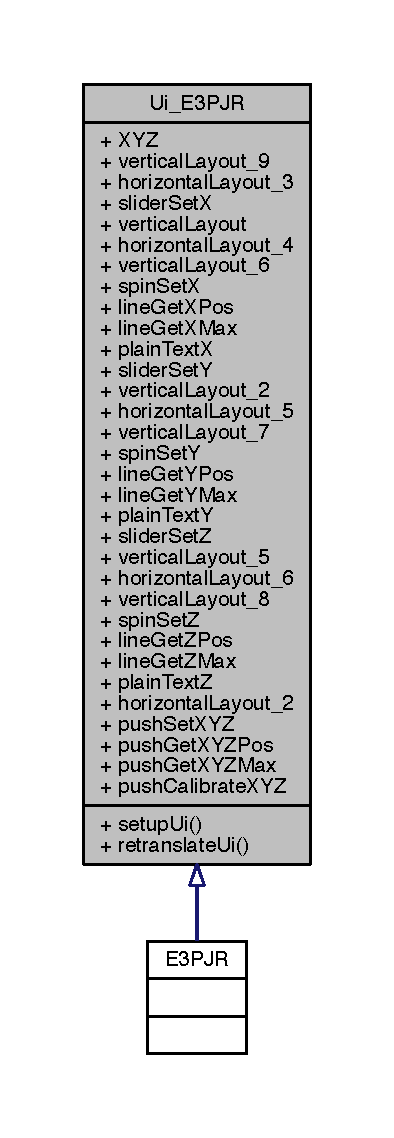
\includegraphics[width=189pt]{d0/d34/class_ui___e3_p_j_r__inherit__graph}
\end{center}
\end{figure}


Samarbejdsdiagram for Ui\+\_\+\+E3\+P\+JR\+:
\nopagebreak
\begin{figure}[H]
\begin{center}
\leavevmode
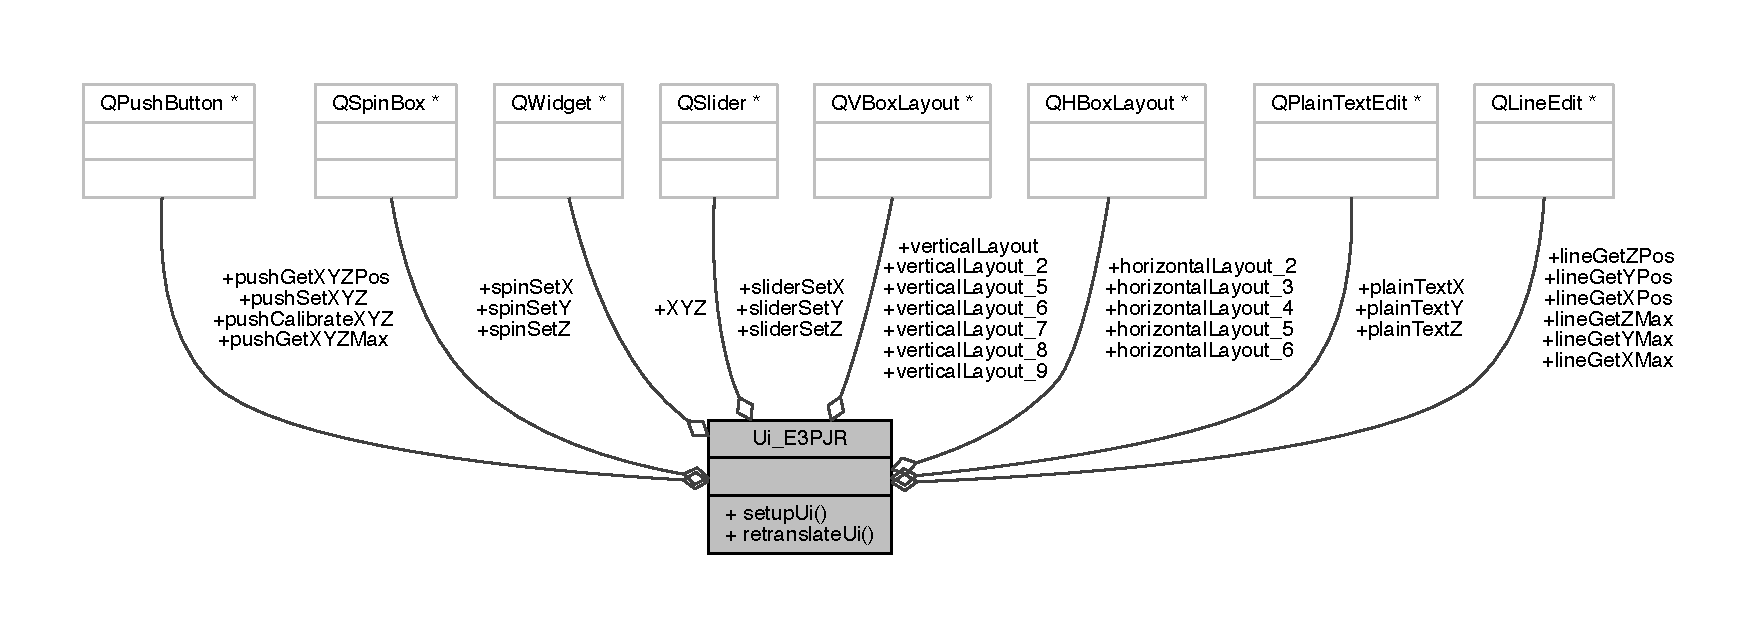
\includegraphics[width=350pt]{dd/d9a/class_ui___e3_p_j_r__coll__graph}
\end{center}
\end{figure}
\subsubsection*{Offentlige metoder}
\begin{DoxyCompactItemize}
\item 
void \hyperlink{class_ui___e3_p_j_r_acd00a207b203ce4e08e2d4fe020281d2}{setup\+Ui} (\hyperlink{class_q_tab_widget}{Q\+Tab\+Widget} $\ast$\hyperlink{class_e3_p_j_r}{E3\+P\+JR})
\item 
void \hyperlink{class_ui___e3_p_j_r_ab4d1867d3517a19d5b74c57ffd921202}{retranslate\+Ui} (\hyperlink{class_q_tab_widget}{Q\+Tab\+Widget} $\ast$\hyperlink{class_e3_p_j_r}{E3\+P\+JR})
\end{DoxyCompactItemize}
\subsubsection*{Datafelter}
\begin{DoxyCompactItemize}
\item 
\hyperlink{class_q_widget}{Q\+Widget} $\ast$ \hyperlink{class_ui___e3_p_j_r_a098a80b873d9e0a09fd834f09e5028b4}{X\+YZ}
\item 
Q\+V\+Box\+Layout $\ast$ \hyperlink{class_ui___e3_p_j_r_a7c00a0b53a83fa0709131b996a6249a9}{vertical\+Layout\+\_\+9}
\item 
Q\+H\+Box\+Layout $\ast$ \hyperlink{class_ui___e3_p_j_r_af1b2167ad3027fe2c2328701164e54ec}{horizontal\+Layout\+\_\+3}
\item 
Q\+Slider $\ast$ \hyperlink{class_ui___e3_p_j_r_ac45c355780da0c571a472ccb5f74c977}{slider\+SetX}
\item 
Q\+V\+Box\+Layout $\ast$ \hyperlink{class_ui___e3_p_j_r_ad85f9339d941aa92fe82db7dcba6664c}{vertical\+Layout}
\item 
Q\+H\+Box\+Layout $\ast$ \hyperlink{class_ui___e3_p_j_r_aeb3eff1a8b0673c92f1ed957263d272b}{horizontal\+Layout\+\_\+4}
\item 
Q\+V\+Box\+Layout $\ast$ \hyperlink{class_ui___e3_p_j_r_a123f4222372065593b6a3433ac1dde9d}{vertical\+Layout\+\_\+6}
\item 
Q\+Spin\+Box $\ast$ \hyperlink{class_ui___e3_p_j_r_ab782845855d3c29e2d229ff09b717771}{spin\+SetX}
\item 
Q\+Line\+Edit $\ast$ \hyperlink{class_ui___e3_p_j_r_a2aa996a4bf178178f8c776bd139e1e98}{line\+Get\+X\+Pos}
\item 
Q\+Line\+Edit $\ast$ \hyperlink{class_ui___e3_p_j_r_aa70a702ff832048eb7b3a06560b1cccd}{line\+Get\+X\+Max}
\item 
Q\+Plain\+Text\+Edit $\ast$ \hyperlink{class_ui___e3_p_j_r_ac06b3dba512fbdc4436a33323fd6e737}{plain\+TextX}
\item 
Q\+Slider $\ast$ \hyperlink{class_ui___e3_p_j_r_afc14eb4b41f896c3881b1f3f86ebb5ab}{slider\+SetY}
\item 
Q\+V\+Box\+Layout $\ast$ \hyperlink{class_ui___e3_p_j_r_a1f81b7e95162efcbe551b64ca41869c8}{vertical\+Layout\+\_\+2}
\item 
Q\+H\+Box\+Layout $\ast$ \hyperlink{class_ui___e3_p_j_r_a9200504b29bbbfa17f9e6aefafc2c122}{horizontal\+Layout\+\_\+5}
\item 
Q\+V\+Box\+Layout $\ast$ \hyperlink{class_ui___e3_p_j_r_a6846ec6f18ab0ea13bdb2d00b2cb3947}{vertical\+Layout\+\_\+7}
\item 
Q\+Spin\+Box $\ast$ \hyperlink{class_ui___e3_p_j_r_a855f6972ba1dc6a61308080e1dea2447}{spin\+SetY}
\item 
Q\+Line\+Edit $\ast$ \hyperlink{class_ui___e3_p_j_r_af7a504d650e35e560d66d6e9cc2ec20e}{line\+Get\+Y\+Pos}
\item 
Q\+Line\+Edit $\ast$ \hyperlink{class_ui___e3_p_j_r_a6db76c359ac491d1e084a0febda62fa8}{line\+Get\+Y\+Max}
\item 
Q\+Plain\+Text\+Edit $\ast$ \hyperlink{class_ui___e3_p_j_r_aded895240a26d5b3349be548e863fcd2}{plain\+TextY}
\item 
Q\+Slider $\ast$ \hyperlink{class_ui___e3_p_j_r_a6ef8bc7a96e71c14d44d1573f43506d4}{slider\+SetZ}
\item 
Q\+V\+Box\+Layout $\ast$ \hyperlink{class_ui___e3_p_j_r_acbe0600e63ca9c63fe807730289e677a}{vertical\+Layout\+\_\+5}
\item 
Q\+H\+Box\+Layout $\ast$ \hyperlink{class_ui___e3_p_j_r_aee7bbbb4f14e80e5c3821623d9c4d52b}{horizontal\+Layout\+\_\+6}
\item 
Q\+V\+Box\+Layout $\ast$ \hyperlink{class_ui___e3_p_j_r_aecbd2cafbe12abcd4a5a7865aad8d917}{vertical\+Layout\+\_\+8}
\item 
Q\+Spin\+Box $\ast$ \hyperlink{class_ui___e3_p_j_r_a1c5f1bef8dc94bae1a91139a37d1d881}{spin\+SetZ}
\item 
Q\+Line\+Edit $\ast$ \hyperlink{class_ui___e3_p_j_r_af271cd40f5223cbdb1803e41493746cc}{line\+Get\+Z\+Pos}
\item 
Q\+Line\+Edit $\ast$ \hyperlink{class_ui___e3_p_j_r_a4bd5e082a2fb51522d5606ed355289d5}{line\+Get\+Z\+Max}
\item 
Q\+Plain\+Text\+Edit $\ast$ \hyperlink{class_ui___e3_p_j_r_aa688da4507156fb25ab31678d45842c9}{plain\+TextZ}
\item 
Q\+H\+Box\+Layout $\ast$ \hyperlink{class_ui___e3_p_j_r_a535a43287b7a5605cfc11580d146d3fb}{horizontal\+Layout\+\_\+2}
\item 
Q\+Push\+Button $\ast$ \hyperlink{class_ui___e3_p_j_r_a95989982eaebbf117db602b9c5642fc5}{push\+Set\+X\+YZ}
\item 
Q\+Push\+Button $\ast$ \hyperlink{class_ui___e3_p_j_r_a5a172ff2cdd7f0b1731e866267981cd4}{push\+Get\+X\+Y\+Z\+Pos}
\item 
Q\+Push\+Button $\ast$ \hyperlink{class_ui___e3_p_j_r_a16f1701307e43c614a3c0aed623577b7}{push\+Get\+X\+Y\+Z\+Max}
\item 
Q\+Push\+Button $\ast$ \hyperlink{class_ui___e3_p_j_r_a0a82bc71b94b2c607f872cbcf936811a}{push\+Calibrate\+X\+YZ}
\end{DoxyCompactItemize}


\subsubsection{Detaljeret beskrivelse}


Defineret på linje 29 i filen ui\+\_\+e3pjr.\+h.



\subsubsection{Dokumentation af medlemsfunktioner}
\index{Ui\+\_\+\+E3\+P\+JR@{Ui\+\_\+\+E3\+P\+JR}!retranslate\+Ui@{retranslate\+Ui}}
\index{retranslate\+Ui@{retranslate\+Ui}!Ui\+\_\+\+E3\+P\+JR@{Ui\+\_\+\+E3\+P\+JR}}
\paragraph[{\texorpdfstring{retranslate\+Ui(\+Q\+Tab\+Widget $\ast$\+E3\+P\+J\+R)}{retranslateUi(QTabWidget *E3PJR)}}]{\setlength{\rightskip}{0pt plus 5cm}void retranslate\+Ui (
\begin{DoxyParamCaption}
\item[{{\bf Q\+Tab\+Widget} $\ast$}]{E3\+P\+JR}
\end{DoxyParamCaption}
)\hspace{0.3cm}{\ttfamily [inline]}}\hypertarget{class_ui___e3_p_j_r_ab4d1867d3517a19d5b74c57ffd921202}{}\label{class_ui___e3_p_j_r_ab4d1867d3517a19d5b74c57ffd921202}


Defineret på linje 281 i filen ui\+\_\+e3pjr.\+h.



Refereret til af setup\+Ui().


\begin{DoxyCode}
282     \{
283         E3PJR->setWindowTitle(QApplication::translate(\textcolor{stringliteral}{"E3PJR"}, \textcolor{stringliteral}{"TabWidget"}, 0, QApplication::UnicodeUTF8));
284         \hyperlink{class_ui___e3_p_j_r_a2aa996a4bf178178f8c776bd139e1e98}{lineGetXPos}->setPlaceholderText(QApplication::translate(\textcolor{stringliteral}{"E3PJR"}, \textcolor{stringliteral}{"xPos"}, 0, 
      QApplication::UnicodeUTF8));
285         \hyperlink{class_ui___e3_p_j_r_aa70a702ff832048eb7b3a06560b1cccd}{lineGetXMax}->setPlaceholderText(QApplication::translate(\textcolor{stringliteral}{"E3PJR"}, \textcolor{stringliteral}{"xMax"}, 0, 
      QApplication::UnicodeUTF8));
286         \hyperlink{class_ui___e3_p_j_r_af7a504d650e35e560d66d6e9cc2ec20e}{lineGetYPos}->setPlaceholderText(QApplication::translate(\textcolor{stringliteral}{"E3PJR"}, \textcolor{stringliteral}{"yPos"}, 0, 
      QApplication::UnicodeUTF8));
287         \hyperlink{class_ui___e3_p_j_r_a6db76c359ac491d1e084a0febda62fa8}{lineGetYMax}->setPlaceholderText(QApplication::translate(\textcolor{stringliteral}{"E3PJR"}, \textcolor{stringliteral}{"yMax"}, 0, 
      QApplication::UnicodeUTF8));
288         \hyperlink{class_ui___e3_p_j_r_af271cd40f5223cbdb1803e41493746cc}{lineGetZPos}->setPlaceholderText(QApplication::translate(\textcolor{stringliteral}{"E3PJR"}, \textcolor{stringliteral}{"zPos"}, 0, 
      QApplication::UnicodeUTF8));
289         \hyperlink{class_ui___e3_p_j_r_a4bd5e082a2fb51522d5606ed355289d5}{lineGetZMax}->setPlaceholderText(QApplication::translate(\textcolor{stringliteral}{"E3PJR"}, \textcolor{stringliteral}{"zMax"}, 0, 
      QApplication::UnicodeUTF8));
290         \hyperlink{class_ui___e3_p_j_r_a95989982eaebbf117db602b9c5642fc5}{pushSetXYZ}->setText(QApplication::translate(\textcolor{stringliteral}{"E3PJR"}, \textcolor{stringliteral}{"SetXYZPos"}, 0, 
      QApplication::UnicodeUTF8));
291         \hyperlink{class_ui___e3_p_j_r_a5a172ff2cdd7f0b1731e866267981cd4}{pushGetXYZPos}->setText(QApplication::translate(\textcolor{stringliteral}{"E3PJR"}, \textcolor{stringliteral}{"GetXYZPos"}, 0, 
      QApplication::UnicodeUTF8));
292         \hyperlink{class_ui___e3_p_j_r_a16f1701307e43c614a3c0aed623577b7}{pushGetXYZMax}->setText(QApplication::translate(\textcolor{stringliteral}{"E3PJR"}, \textcolor{stringliteral}{"GetXYZMax"}, 0, 
      QApplication::UnicodeUTF8));
293         \hyperlink{class_ui___e3_p_j_r_a0a82bc71b94b2c607f872cbcf936811a}{pushCalibrateXYZ}->setText(QApplication::translate(\textcolor{stringliteral}{"E3PJR"}, \textcolor{stringliteral}{"CalibrateXYZ"}, 0, 
      QApplication::UnicodeUTF8));
294         E3PJR->setTabText(E3PJR->indexOf(\hyperlink{class_ui___e3_p_j_r_a098a80b873d9e0a09fd834f09e5028b4}{XYZ}), QApplication::translate(\textcolor{stringliteral}{"E3PJR"}, \textcolor{stringliteral}{"XYZ"}, 0, 
      QApplication::UnicodeUTF8));
295     \} \textcolor{comment}{// retranslateUi}
\end{DoxyCode}


Her er kalder-\/grafen for denne funktion\+:
\nopagebreak
\begin{figure}[H]
\begin{center}
\leavevmode
\includegraphics[width=239pt]{db/de3/class_ui___e3_p_j_r_ab4d1867d3517a19d5b74c57ffd921202_icgraph}
\end{center}
\end{figure}


\index{Ui\+\_\+\+E3\+P\+JR@{Ui\+\_\+\+E3\+P\+JR}!setup\+Ui@{setup\+Ui}}
\index{setup\+Ui@{setup\+Ui}!Ui\+\_\+\+E3\+P\+JR@{Ui\+\_\+\+E3\+P\+JR}}
\paragraph[{\texorpdfstring{setup\+Ui(\+Q\+Tab\+Widget $\ast$\+E3\+P\+J\+R)}{setupUi(QTabWidget *E3PJR)}}]{\setlength{\rightskip}{0pt plus 5cm}void setup\+Ui (
\begin{DoxyParamCaption}
\item[{{\bf Q\+Tab\+Widget} $\ast$}]{E3\+P\+JR}
\end{DoxyParamCaption}
)\hspace{0.3cm}{\ttfamily [inline]}}\hypertarget{class_ui___e3_p_j_r_acd00a207b203ce4e08e2d4fe020281d2}{}\label{class_ui___e3_p_j_r_acd00a207b203ce4e08e2d4fe020281d2}


Defineret på linje 65 i filen ui\+\_\+e3pjr.\+h.



Indeholder referencer til retranslate\+Ui().


\begin{DoxyCode}
66     \{
67         \textcolor{keywordflow}{if} (E3PJR->objectName().isEmpty())
68             E3PJR->setObjectName(QString::fromUtf8(\textcolor{stringliteral}{"E3PJR"}));
69         E3PJR->resize(480, 278);
70         \hyperlink{class_ui___e3_p_j_r_a098a80b873d9e0a09fd834f09e5028b4}{XYZ} = \textcolor{keyword}{new} \hyperlink{class_q_widget}{QWidget}();
71         \hyperlink{class_ui___e3_p_j_r_a098a80b873d9e0a09fd834f09e5028b4}{XYZ}->setObjectName(QString::fromUtf8(\textcolor{stringliteral}{"XYZ"}));
72         \hyperlink{class_ui___e3_p_j_r_a7c00a0b53a83fa0709131b996a6249a9}{verticalLayout\_9} = \textcolor{keyword}{new} QVBoxLayout(\hyperlink{class_ui___e3_p_j_r_a098a80b873d9e0a09fd834f09e5028b4}{XYZ});
73         \hyperlink{class_ui___e3_p_j_r_a7c00a0b53a83fa0709131b996a6249a9}{verticalLayout\_9}->setObjectName(QString::fromUtf8(\textcolor{stringliteral}{"verticalLayout\_9"}));
74         \hyperlink{class_ui___e3_p_j_r_af1b2167ad3027fe2c2328701164e54ec}{horizontalLayout\_3} = \textcolor{keyword}{new} QHBoxLayout();
75         \hyperlink{class_ui___e3_p_j_r_af1b2167ad3027fe2c2328701164e54ec}{horizontalLayout\_3}->setObjectName(QString::fromUtf8(\textcolor{stringliteral}{"horizontalLayout\_3"}));
76         \hyperlink{class_ui___e3_p_j_r_ac45c355780da0c571a472ccb5f74c977}{sliderSetX} = \textcolor{keyword}{new} QSlider(\hyperlink{class_ui___e3_p_j_r_a098a80b873d9e0a09fd834f09e5028b4}{XYZ});
77         \hyperlink{class_ui___e3_p_j_r_ac45c355780da0c571a472ccb5f74c977}{sliderSetX}->setObjectName(QString::fromUtf8(\textcolor{stringliteral}{"sliderSetX"}));
78         \hyperlink{class_ui___e3_p_j_r_ac45c355780da0c571a472ccb5f74c977}{sliderSetX}->setMaximum(255);
79         \hyperlink{class_ui___e3_p_j_r_ac45c355780da0c571a472ccb5f74c977}{sliderSetX}->setSingleStep(5);
80         \hyperlink{class_ui___e3_p_j_r_ac45c355780da0c571a472ccb5f74c977}{sliderSetX}->setPageStep(15);
81         \hyperlink{class_ui___e3_p_j_r_ac45c355780da0c571a472ccb5f74c977}{sliderSetX}->setOrientation(Qt::Vertical);
82 
83         \hyperlink{class_ui___e3_p_j_r_af1b2167ad3027fe2c2328701164e54ec}{horizontalLayout\_3}->addWidget(\hyperlink{class_ui___e3_p_j_r_ac45c355780da0c571a472ccb5f74c977}{sliderSetX});
84 
85         \hyperlink{class_ui___e3_p_j_r_ad85f9339d941aa92fe82db7dcba6664c}{verticalLayout} = \textcolor{keyword}{new} QVBoxLayout();
86         \hyperlink{class_ui___e3_p_j_r_ad85f9339d941aa92fe82db7dcba6664c}{verticalLayout}->setObjectName(QString::fromUtf8(\textcolor{stringliteral}{"verticalLayout"}));
87         \hyperlink{class_ui___e3_p_j_r_aeb3eff1a8b0673c92f1ed957263d272b}{horizontalLayout\_4} = \textcolor{keyword}{new} QHBoxLayout();
88         \hyperlink{class_ui___e3_p_j_r_aeb3eff1a8b0673c92f1ed957263d272b}{horizontalLayout\_4}->setObjectName(QString::fromUtf8(\textcolor{stringliteral}{"horizontalLayout\_4"}));
89         \hyperlink{class_ui___e3_p_j_r_a123f4222372065593b6a3433ac1dde9d}{verticalLayout\_6} = \textcolor{keyword}{new} QVBoxLayout();
90         \hyperlink{class_ui___e3_p_j_r_a123f4222372065593b6a3433ac1dde9d}{verticalLayout\_6}->setObjectName(QString::fromUtf8(\textcolor{stringliteral}{"verticalLayout\_6"}));
91         \hyperlink{class_ui___e3_p_j_r_ab782845855d3c29e2d229ff09b717771}{spinSetX} = \textcolor{keyword}{new} QSpinBox(\hyperlink{class_ui___e3_p_j_r_a098a80b873d9e0a09fd834f09e5028b4}{XYZ});
92         \hyperlink{class_ui___e3_p_j_r_ab782845855d3c29e2d229ff09b717771}{spinSetX}->setObjectName(QString::fromUtf8(\textcolor{stringliteral}{"spinSetX"}));
93         \hyperlink{class_ui___e3_p_j_r_ab782845855d3c29e2d229ff09b717771}{spinSetX}->setAlignment(Qt::AlignCenter);
94         \hyperlink{class_ui___e3_p_j_r_ab782845855d3c29e2d229ff09b717771}{spinSetX}->setMaximum(255);
95         \hyperlink{class_ui___e3_p_j_r_ab782845855d3c29e2d229ff09b717771}{spinSetX}->setSingleStep(5);
96 
97         \hyperlink{class_ui___e3_p_j_r_a123f4222372065593b6a3433ac1dde9d}{verticalLayout\_6}->addWidget(\hyperlink{class_ui___e3_p_j_r_ab782845855d3c29e2d229ff09b717771}{spinSetX});
98 
99         \hyperlink{class_ui___e3_p_j_r_a2aa996a4bf178178f8c776bd139e1e98}{lineGetXPos} = \textcolor{keyword}{new} QLineEdit(\hyperlink{class_ui___e3_p_j_r_a098a80b873d9e0a09fd834f09e5028b4}{XYZ});
100         \hyperlink{class_ui___e3_p_j_r_a2aa996a4bf178178f8c776bd139e1e98}{lineGetXPos}->setObjectName(QString::fromUtf8(\textcolor{stringliteral}{"lineGetXPos"}));
101         \hyperlink{class_ui___e3_p_j_r_a2aa996a4bf178178f8c776bd139e1e98}{lineGetXPos}->setAlignment(Qt::AlignCenter);
102 
103         \hyperlink{class_ui___e3_p_j_r_a123f4222372065593b6a3433ac1dde9d}{verticalLayout\_6}->addWidget(\hyperlink{class_ui___e3_p_j_r_a2aa996a4bf178178f8c776bd139e1e98}{lineGetXPos});
104 
105         \hyperlink{class_ui___e3_p_j_r_aa70a702ff832048eb7b3a06560b1cccd}{lineGetXMax} = \textcolor{keyword}{new} QLineEdit(\hyperlink{class_ui___e3_p_j_r_a098a80b873d9e0a09fd834f09e5028b4}{XYZ});
106         \hyperlink{class_ui___e3_p_j_r_aa70a702ff832048eb7b3a06560b1cccd}{lineGetXMax}->setObjectName(QString::fromUtf8(\textcolor{stringliteral}{"lineGetXMax"}));
107         \hyperlink{class_ui___e3_p_j_r_aa70a702ff832048eb7b3a06560b1cccd}{lineGetXMax}->setAlignment(Qt::AlignCenter);
108 
109         \hyperlink{class_ui___e3_p_j_r_a123f4222372065593b6a3433ac1dde9d}{verticalLayout\_6}->addWidget(\hyperlink{class_ui___e3_p_j_r_aa70a702ff832048eb7b3a06560b1cccd}{lineGetXMax});
110 
111 
112         \hyperlink{class_ui___e3_p_j_r_aeb3eff1a8b0673c92f1ed957263d272b}{horizontalLayout\_4}->addLayout(\hyperlink{class_ui___e3_p_j_r_a123f4222372065593b6a3433ac1dde9d}{verticalLayout\_6});
113 
114 
115         \hyperlink{class_ui___e3_p_j_r_ad85f9339d941aa92fe82db7dcba6664c}{verticalLayout}->addLayout(\hyperlink{class_ui___e3_p_j_r_aeb3eff1a8b0673c92f1ed957263d272b}{horizontalLayout\_4});
116 
117         \hyperlink{class_ui___e3_p_j_r_ac06b3dba512fbdc4436a33323fd6e737}{plainTextX} = \textcolor{keyword}{new} QPlainTextEdit(\hyperlink{class_ui___e3_p_j_r_a098a80b873d9e0a09fd834f09e5028b4}{XYZ});
118         \hyperlink{class_ui___e3_p_j_r_ac06b3dba512fbdc4436a33323fd6e737}{plainTextX}->setObjectName(QString::fromUtf8(\textcolor{stringliteral}{"plainTextX"}));
119         \hyperlink{class_ui___e3_p_j_r_ac06b3dba512fbdc4436a33323fd6e737}{plainTextX}->setVerticalScrollBarPolicy(Qt::ScrollBarAlwaysOff);
120         \hyperlink{class_ui___e3_p_j_r_ac06b3dba512fbdc4436a33323fd6e737}{plainTextX}->setHorizontalScrollBarPolicy(Qt::ScrollBarAlwaysOff);
121         \hyperlink{class_ui___e3_p_j_r_ac06b3dba512fbdc4436a33323fd6e737}{plainTextX}->setUndoRedoEnabled(\textcolor{keyword}{false});
122         \hyperlink{class_ui___e3_p_j_r_ac06b3dba512fbdc4436a33323fd6e737}{plainTextX}->setReadOnly(\textcolor{keyword}{true});
123         \hyperlink{class_ui___e3_p_j_r_ac06b3dba512fbdc4436a33323fd6e737}{plainTextX}->setOverwriteMode(\textcolor{keyword}{false});
124 
125         \hyperlink{class_ui___e3_p_j_r_ad85f9339d941aa92fe82db7dcba6664c}{verticalLayout}->addWidget(\hyperlink{class_ui___e3_p_j_r_ac06b3dba512fbdc4436a33323fd6e737}{plainTextX});
126 
127 
128         \hyperlink{class_ui___e3_p_j_r_af1b2167ad3027fe2c2328701164e54ec}{horizontalLayout\_3}->addLayout(\hyperlink{class_ui___e3_p_j_r_ad85f9339d941aa92fe82db7dcba6664c}{verticalLayout});
129 
130         \hyperlink{class_ui___e3_p_j_r_afc14eb4b41f896c3881b1f3f86ebb5ab}{sliderSetY} = \textcolor{keyword}{new} QSlider(\hyperlink{class_ui___e3_p_j_r_a098a80b873d9e0a09fd834f09e5028b4}{XYZ});
131         \hyperlink{class_ui___e3_p_j_r_afc14eb4b41f896c3881b1f3f86ebb5ab}{sliderSetY}->setObjectName(QString::fromUtf8(\textcolor{stringliteral}{"sliderSetY"}));
132         \hyperlink{class_ui___e3_p_j_r_afc14eb4b41f896c3881b1f3f86ebb5ab}{sliderSetY}->setMaximum(255);
133         \hyperlink{class_ui___e3_p_j_r_afc14eb4b41f896c3881b1f3f86ebb5ab}{sliderSetY}->setSingleStep(5);
134         \hyperlink{class_ui___e3_p_j_r_afc14eb4b41f896c3881b1f3f86ebb5ab}{sliderSetY}->setPageStep(15);
135         \hyperlink{class_ui___e3_p_j_r_afc14eb4b41f896c3881b1f3f86ebb5ab}{sliderSetY}->setOrientation(Qt::Vertical);
136 
137         \hyperlink{class_ui___e3_p_j_r_af1b2167ad3027fe2c2328701164e54ec}{horizontalLayout\_3}->addWidget(\hyperlink{class_ui___e3_p_j_r_afc14eb4b41f896c3881b1f3f86ebb5ab}{sliderSetY});
138 
139         \hyperlink{class_ui___e3_p_j_r_a1f81b7e95162efcbe551b64ca41869c8}{verticalLayout\_2} = \textcolor{keyword}{new} QVBoxLayout();
140         \hyperlink{class_ui___e3_p_j_r_a1f81b7e95162efcbe551b64ca41869c8}{verticalLayout\_2}->setObjectName(QString::fromUtf8(\textcolor{stringliteral}{"verticalLayout\_2"}));
141         \hyperlink{class_ui___e3_p_j_r_a9200504b29bbbfa17f9e6aefafc2c122}{horizontalLayout\_5} = \textcolor{keyword}{new} QHBoxLayout();
142         \hyperlink{class_ui___e3_p_j_r_a9200504b29bbbfa17f9e6aefafc2c122}{horizontalLayout\_5}->setObjectName(QString::fromUtf8(\textcolor{stringliteral}{"horizontalLayout\_5"}));
143         \hyperlink{class_ui___e3_p_j_r_a6846ec6f18ab0ea13bdb2d00b2cb3947}{verticalLayout\_7} = \textcolor{keyword}{new} QVBoxLayout();
144         \hyperlink{class_ui___e3_p_j_r_a6846ec6f18ab0ea13bdb2d00b2cb3947}{verticalLayout\_7}->setObjectName(QString::fromUtf8(\textcolor{stringliteral}{"verticalLayout\_7"}));
145         \hyperlink{class_ui___e3_p_j_r_a855f6972ba1dc6a61308080e1dea2447}{spinSetY} = \textcolor{keyword}{new} QSpinBox(\hyperlink{class_ui___e3_p_j_r_a098a80b873d9e0a09fd834f09e5028b4}{XYZ});
146         \hyperlink{class_ui___e3_p_j_r_a855f6972ba1dc6a61308080e1dea2447}{spinSetY}->setObjectName(QString::fromUtf8(\textcolor{stringliteral}{"spinSetY"}));
147         \hyperlink{class_ui___e3_p_j_r_a855f6972ba1dc6a61308080e1dea2447}{spinSetY}->setAlignment(Qt::AlignCenter);
148         \hyperlink{class_ui___e3_p_j_r_a855f6972ba1dc6a61308080e1dea2447}{spinSetY}->setMaximum(255);
149         \hyperlink{class_ui___e3_p_j_r_a855f6972ba1dc6a61308080e1dea2447}{spinSetY}->setSingleStep(5);
150 
151         \hyperlink{class_ui___e3_p_j_r_a6846ec6f18ab0ea13bdb2d00b2cb3947}{verticalLayout\_7}->addWidget(\hyperlink{class_ui___e3_p_j_r_a855f6972ba1dc6a61308080e1dea2447}{spinSetY});
152 
153         \hyperlink{class_ui___e3_p_j_r_af7a504d650e35e560d66d6e9cc2ec20e}{lineGetYPos} = \textcolor{keyword}{new} QLineEdit(\hyperlink{class_ui___e3_p_j_r_a098a80b873d9e0a09fd834f09e5028b4}{XYZ});
154         \hyperlink{class_ui___e3_p_j_r_af7a504d650e35e560d66d6e9cc2ec20e}{lineGetYPos}->setObjectName(QString::fromUtf8(\textcolor{stringliteral}{"lineGetYPos"}));
155         \hyperlink{class_ui___e3_p_j_r_af7a504d650e35e560d66d6e9cc2ec20e}{lineGetYPos}->setAlignment(Qt::AlignCenter);
156 
157         \hyperlink{class_ui___e3_p_j_r_a6846ec6f18ab0ea13bdb2d00b2cb3947}{verticalLayout\_7}->addWidget(\hyperlink{class_ui___e3_p_j_r_af7a504d650e35e560d66d6e9cc2ec20e}{lineGetYPos});
158 
159         \hyperlink{class_ui___e3_p_j_r_a6db76c359ac491d1e084a0febda62fa8}{lineGetYMax} = \textcolor{keyword}{new} QLineEdit(\hyperlink{class_ui___e3_p_j_r_a098a80b873d9e0a09fd834f09e5028b4}{XYZ});
160         \hyperlink{class_ui___e3_p_j_r_a6db76c359ac491d1e084a0febda62fa8}{lineGetYMax}->setObjectName(QString::fromUtf8(\textcolor{stringliteral}{"lineGetYMax"}));
161         \hyperlink{class_ui___e3_p_j_r_a6db76c359ac491d1e084a0febda62fa8}{lineGetYMax}->setAlignment(Qt::AlignCenter);
162 
163         \hyperlink{class_ui___e3_p_j_r_a6846ec6f18ab0ea13bdb2d00b2cb3947}{verticalLayout\_7}->addWidget(\hyperlink{class_ui___e3_p_j_r_a6db76c359ac491d1e084a0febda62fa8}{lineGetYMax});
164 
165 
166         \hyperlink{class_ui___e3_p_j_r_a9200504b29bbbfa17f9e6aefafc2c122}{horizontalLayout\_5}->addLayout(\hyperlink{class_ui___e3_p_j_r_a6846ec6f18ab0ea13bdb2d00b2cb3947}{verticalLayout\_7});
167 
168 
169         \hyperlink{class_ui___e3_p_j_r_a1f81b7e95162efcbe551b64ca41869c8}{verticalLayout\_2}->addLayout(\hyperlink{class_ui___e3_p_j_r_a9200504b29bbbfa17f9e6aefafc2c122}{horizontalLayout\_5});
170 
171         \hyperlink{class_ui___e3_p_j_r_aded895240a26d5b3349be548e863fcd2}{plainTextY} = \textcolor{keyword}{new} QPlainTextEdit(\hyperlink{class_ui___e3_p_j_r_a098a80b873d9e0a09fd834f09e5028b4}{XYZ});
172         \hyperlink{class_ui___e3_p_j_r_aded895240a26d5b3349be548e863fcd2}{plainTextY}->setObjectName(QString::fromUtf8(\textcolor{stringliteral}{"plainTextY"}));
173         \hyperlink{class_ui___e3_p_j_r_aded895240a26d5b3349be548e863fcd2}{plainTextY}->setVerticalScrollBarPolicy(Qt::ScrollBarAlwaysOff);
174         \hyperlink{class_ui___e3_p_j_r_aded895240a26d5b3349be548e863fcd2}{plainTextY}->setHorizontalScrollBarPolicy(Qt::ScrollBarAlwaysOff);
175         \hyperlink{class_ui___e3_p_j_r_aded895240a26d5b3349be548e863fcd2}{plainTextY}->setUndoRedoEnabled(\textcolor{keyword}{false});
176         \hyperlink{class_ui___e3_p_j_r_aded895240a26d5b3349be548e863fcd2}{plainTextY}->setReadOnly(\textcolor{keyword}{true});
177 
178         \hyperlink{class_ui___e3_p_j_r_a1f81b7e95162efcbe551b64ca41869c8}{verticalLayout\_2}->addWidget(\hyperlink{class_ui___e3_p_j_r_aded895240a26d5b3349be548e863fcd2}{plainTextY});
179 
180 
181         \hyperlink{class_ui___e3_p_j_r_af1b2167ad3027fe2c2328701164e54ec}{horizontalLayout\_3}->addLayout(\hyperlink{class_ui___e3_p_j_r_a1f81b7e95162efcbe551b64ca41869c8}{verticalLayout\_2});
182 
183         \hyperlink{class_ui___e3_p_j_r_a6ef8bc7a96e71c14d44d1573f43506d4}{sliderSetZ} = \textcolor{keyword}{new} QSlider(\hyperlink{class_ui___e3_p_j_r_a098a80b873d9e0a09fd834f09e5028b4}{XYZ});
184         \hyperlink{class_ui___e3_p_j_r_a6ef8bc7a96e71c14d44d1573f43506d4}{sliderSetZ}->setObjectName(QString::fromUtf8(\textcolor{stringliteral}{"sliderSetZ"}));
185         \hyperlink{class_ui___e3_p_j_r_a6ef8bc7a96e71c14d44d1573f43506d4}{sliderSetZ}->setMaximum(255);
186         \hyperlink{class_ui___e3_p_j_r_a6ef8bc7a96e71c14d44d1573f43506d4}{sliderSetZ}->setSingleStep(5);
187         \hyperlink{class_ui___e3_p_j_r_a6ef8bc7a96e71c14d44d1573f43506d4}{sliderSetZ}->setPageStep(15);
188         \hyperlink{class_ui___e3_p_j_r_a6ef8bc7a96e71c14d44d1573f43506d4}{sliderSetZ}->setOrientation(Qt::Vertical);
189 
190         \hyperlink{class_ui___e3_p_j_r_af1b2167ad3027fe2c2328701164e54ec}{horizontalLayout\_3}->addWidget(\hyperlink{class_ui___e3_p_j_r_a6ef8bc7a96e71c14d44d1573f43506d4}{sliderSetZ});
191 
192         \hyperlink{class_ui___e3_p_j_r_acbe0600e63ca9c63fe807730289e677a}{verticalLayout\_5} = \textcolor{keyword}{new} QVBoxLayout();
193         \hyperlink{class_ui___e3_p_j_r_acbe0600e63ca9c63fe807730289e677a}{verticalLayout\_5}->setObjectName(QString::fromUtf8(\textcolor{stringliteral}{"verticalLayout\_5"}));
194         \hyperlink{class_ui___e3_p_j_r_aee7bbbb4f14e80e5c3821623d9c4d52b}{horizontalLayout\_6} = \textcolor{keyword}{new} QHBoxLayout();
195         \hyperlink{class_ui___e3_p_j_r_aee7bbbb4f14e80e5c3821623d9c4d52b}{horizontalLayout\_6}->setObjectName(QString::fromUtf8(\textcolor{stringliteral}{"horizontalLayout\_6"}));
196         \hyperlink{class_ui___e3_p_j_r_aecbd2cafbe12abcd4a5a7865aad8d917}{verticalLayout\_8} = \textcolor{keyword}{new} QVBoxLayout();
197         \hyperlink{class_ui___e3_p_j_r_aecbd2cafbe12abcd4a5a7865aad8d917}{verticalLayout\_8}->setObjectName(QString::fromUtf8(\textcolor{stringliteral}{"verticalLayout\_8"}));
198         \hyperlink{class_ui___e3_p_j_r_a1c5f1bef8dc94bae1a91139a37d1d881}{spinSetZ} = \textcolor{keyword}{new} QSpinBox(\hyperlink{class_ui___e3_p_j_r_a098a80b873d9e0a09fd834f09e5028b4}{XYZ});
199         \hyperlink{class_ui___e3_p_j_r_a1c5f1bef8dc94bae1a91139a37d1d881}{spinSetZ}->setObjectName(QString::fromUtf8(\textcolor{stringliteral}{"spinSetZ"}));
200         \hyperlink{class_ui___e3_p_j_r_a1c5f1bef8dc94bae1a91139a37d1d881}{spinSetZ}->setAlignment(Qt::AlignCenter);
201         \hyperlink{class_ui___e3_p_j_r_a1c5f1bef8dc94bae1a91139a37d1d881}{spinSetZ}->setMaximum(255);
202         \hyperlink{class_ui___e3_p_j_r_a1c5f1bef8dc94bae1a91139a37d1d881}{spinSetZ}->setSingleStep(5);
203 
204         \hyperlink{class_ui___e3_p_j_r_aecbd2cafbe12abcd4a5a7865aad8d917}{verticalLayout\_8}->addWidget(\hyperlink{class_ui___e3_p_j_r_a1c5f1bef8dc94bae1a91139a37d1d881}{spinSetZ});
205 
206         \hyperlink{class_ui___e3_p_j_r_af271cd40f5223cbdb1803e41493746cc}{lineGetZPos} = \textcolor{keyword}{new} QLineEdit(\hyperlink{class_ui___e3_p_j_r_a098a80b873d9e0a09fd834f09e5028b4}{XYZ});
207         \hyperlink{class_ui___e3_p_j_r_af271cd40f5223cbdb1803e41493746cc}{lineGetZPos}->setObjectName(QString::fromUtf8(\textcolor{stringliteral}{"lineGetZPos"}));
208         \hyperlink{class_ui___e3_p_j_r_af271cd40f5223cbdb1803e41493746cc}{lineGetZPos}->setAlignment(Qt::AlignCenter);
209 
210         \hyperlink{class_ui___e3_p_j_r_aecbd2cafbe12abcd4a5a7865aad8d917}{verticalLayout\_8}->addWidget(\hyperlink{class_ui___e3_p_j_r_af271cd40f5223cbdb1803e41493746cc}{lineGetZPos});
211 
212         \hyperlink{class_ui___e3_p_j_r_a4bd5e082a2fb51522d5606ed355289d5}{lineGetZMax} = \textcolor{keyword}{new} QLineEdit(\hyperlink{class_ui___e3_p_j_r_a098a80b873d9e0a09fd834f09e5028b4}{XYZ});
213         \hyperlink{class_ui___e3_p_j_r_a4bd5e082a2fb51522d5606ed355289d5}{lineGetZMax}->setObjectName(QString::fromUtf8(\textcolor{stringliteral}{"lineGetZMax"}));
214         \hyperlink{class_ui___e3_p_j_r_a4bd5e082a2fb51522d5606ed355289d5}{lineGetZMax}->setAlignment(Qt::AlignCenter);
215 
216         \hyperlink{class_ui___e3_p_j_r_aecbd2cafbe12abcd4a5a7865aad8d917}{verticalLayout\_8}->addWidget(\hyperlink{class_ui___e3_p_j_r_a4bd5e082a2fb51522d5606ed355289d5}{lineGetZMax});
217 
218 
219         \hyperlink{class_ui___e3_p_j_r_aee7bbbb4f14e80e5c3821623d9c4d52b}{horizontalLayout\_6}->addLayout(\hyperlink{class_ui___e3_p_j_r_aecbd2cafbe12abcd4a5a7865aad8d917}{verticalLayout\_8});
220 
221 
222         \hyperlink{class_ui___e3_p_j_r_acbe0600e63ca9c63fe807730289e677a}{verticalLayout\_5}->addLayout(\hyperlink{class_ui___e3_p_j_r_aee7bbbb4f14e80e5c3821623d9c4d52b}{horizontalLayout\_6});
223 
224         \hyperlink{class_ui___e3_p_j_r_aa688da4507156fb25ab31678d45842c9}{plainTextZ} = \textcolor{keyword}{new} QPlainTextEdit(\hyperlink{class_ui___e3_p_j_r_a098a80b873d9e0a09fd834f09e5028b4}{XYZ});
225         \hyperlink{class_ui___e3_p_j_r_aa688da4507156fb25ab31678d45842c9}{plainTextZ}->setObjectName(QString::fromUtf8(\textcolor{stringliteral}{"plainTextZ"}));
226         \hyperlink{class_ui___e3_p_j_r_aa688da4507156fb25ab31678d45842c9}{plainTextZ}->setVerticalScrollBarPolicy(Qt::ScrollBarAlwaysOff);
227         \hyperlink{class_ui___e3_p_j_r_aa688da4507156fb25ab31678d45842c9}{plainTextZ}->setHorizontalScrollBarPolicy(Qt::ScrollBarAlwaysOff);
228         \hyperlink{class_ui___e3_p_j_r_aa688da4507156fb25ab31678d45842c9}{plainTextZ}->setUndoRedoEnabled(\textcolor{keyword}{false});
229         \hyperlink{class_ui___e3_p_j_r_aa688da4507156fb25ab31678d45842c9}{plainTextZ}->setReadOnly(\textcolor{keyword}{true});
230 
231         \hyperlink{class_ui___e3_p_j_r_acbe0600e63ca9c63fe807730289e677a}{verticalLayout\_5}->addWidget(\hyperlink{class_ui___e3_p_j_r_aa688da4507156fb25ab31678d45842c9}{plainTextZ});
232 
233 
234         \hyperlink{class_ui___e3_p_j_r_af1b2167ad3027fe2c2328701164e54ec}{horizontalLayout\_3}->addLayout(\hyperlink{class_ui___e3_p_j_r_acbe0600e63ca9c63fe807730289e677a}{verticalLayout\_5});
235 
236 
237         \hyperlink{class_ui___e3_p_j_r_a7c00a0b53a83fa0709131b996a6249a9}{verticalLayout\_9}->addLayout(\hyperlink{class_ui___e3_p_j_r_af1b2167ad3027fe2c2328701164e54ec}{horizontalLayout\_3});
238 
239         \hyperlink{class_ui___e3_p_j_r_a535a43287b7a5605cfc11580d146d3fb}{horizontalLayout\_2} = \textcolor{keyword}{new} QHBoxLayout();
240         \hyperlink{class_ui___e3_p_j_r_a535a43287b7a5605cfc11580d146d3fb}{horizontalLayout\_2}->setObjectName(QString::fromUtf8(\textcolor{stringliteral}{"horizontalLayout\_2"}));
241         \hyperlink{class_ui___e3_p_j_r_a95989982eaebbf117db602b9c5642fc5}{pushSetXYZ} = \textcolor{keyword}{new} QPushButton(\hyperlink{class_ui___e3_p_j_r_a098a80b873d9e0a09fd834f09e5028b4}{XYZ});
242         \hyperlink{class_ui___e3_p_j_r_a95989982eaebbf117db602b9c5642fc5}{pushSetXYZ}->setObjectName(QString::fromUtf8(\textcolor{stringliteral}{"pushSetXYZ"}));
243 
244         \hyperlink{class_ui___e3_p_j_r_a535a43287b7a5605cfc11580d146d3fb}{horizontalLayout\_2}->addWidget(\hyperlink{class_ui___e3_p_j_r_a95989982eaebbf117db602b9c5642fc5}{pushSetXYZ});
245 
246         \hyperlink{class_ui___e3_p_j_r_a5a172ff2cdd7f0b1731e866267981cd4}{pushGetXYZPos} = \textcolor{keyword}{new} QPushButton(\hyperlink{class_ui___e3_p_j_r_a098a80b873d9e0a09fd834f09e5028b4}{XYZ});
247         \hyperlink{class_ui___e3_p_j_r_a5a172ff2cdd7f0b1731e866267981cd4}{pushGetXYZPos}->setObjectName(QString::fromUtf8(\textcolor{stringliteral}{"pushGetXYZPos"}));
248 
249         \hyperlink{class_ui___e3_p_j_r_a535a43287b7a5605cfc11580d146d3fb}{horizontalLayout\_2}->addWidget(\hyperlink{class_ui___e3_p_j_r_a5a172ff2cdd7f0b1731e866267981cd4}{pushGetXYZPos});
250 
251         \hyperlink{class_ui___e3_p_j_r_a16f1701307e43c614a3c0aed623577b7}{pushGetXYZMax} = \textcolor{keyword}{new} QPushButton(\hyperlink{class_ui___e3_p_j_r_a098a80b873d9e0a09fd834f09e5028b4}{XYZ});
252         \hyperlink{class_ui___e3_p_j_r_a16f1701307e43c614a3c0aed623577b7}{pushGetXYZMax}->setObjectName(QString::fromUtf8(\textcolor{stringliteral}{"pushGetXYZMax"}));
253 
254         \hyperlink{class_ui___e3_p_j_r_a535a43287b7a5605cfc11580d146d3fb}{horizontalLayout\_2}->addWidget(\hyperlink{class_ui___e3_p_j_r_a16f1701307e43c614a3c0aed623577b7}{pushGetXYZMax});
255 
256         \hyperlink{class_ui___e3_p_j_r_a0a82bc71b94b2c607f872cbcf936811a}{pushCalibrateXYZ} = \textcolor{keyword}{new} QPushButton(\hyperlink{class_ui___e3_p_j_r_a098a80b873d9e0a09fd834f09e5028b4}{XYZ});
257         \hyperlink{class_ui___e3_p_j_r_a0a82bc71b94b2c607f872cbcf936811a}{pushCalibrateXYZ}->setObjectName(QString::fromUtf8(\textcolor{stringliteral}{"pushCalibrateXYZ"}));
258 
259         \hyperlink{class_ui___e3_p_j_r_a535a43287b7a5605cfc11580d146d3fb}{horizontalLayout\_2}->addWidget(\hyperlink{class_ui___e3_p_j_r_a0a82bc71b94b2c607f872cbcf936811a}{pushCalibrateXYZ});
260 
261 
262         \hyperlink{class_ui___e3_p_j_r_a7c00a0b53a83fa0709131b996a6249a9}{verticalLayout\_9}->addLayout(\hyperlink{class_ui___e3_p_j_r_a535a43287b7a5605cfc11580d146d3fb}{horizontalLayout\_2});
263 
264         E3PJR->addTab(\hyperlink{class_ui___e3_p_j_r_a098a80b873d9e0a09fd834f09e5028b4}{XYZ}, QString());
265         QWidget::setTabOrder(\hyperlink{class_ui___e3_p_j_r_a855f6972ba1dc6a61308080e1dea2447}{spinSetY}, \hyperlink{class_ui___e3_p_j_r_a1c5f1bef8dc94bae1a91139a37d1d881}{spinSetZ});
266 
267         \hyperlink{class_ui___e3_p_j_r_ab4d1867d3517a19d5b74c57ffd921202}{retranslateUi}(E3PJR);
268         QObject::connect(\hyperlink{class_ui___e3_p_j_r_afc14eb4b41f896c3881b1f3f86ebb5ab}{sliderSetY}, SIGNAL(valueChanged(\textcolor{keywordtype}{int})), 
      \hyperlink{class_ui___e3_p_j_r_a855f6972ba1dc6a61308080e1dea2447}{spinSetY}, SLOT(setValue(\textcolor{keywordtype}{int})));
269         QObject::connect(\hyperlink{class_ui___e3_p_j_r_a855f6972ba1dc6a61308080e1dea2447}{spinSetY}, SIGNAL(valueChanged(\textcolor{keywordtype}{int})), \hyperlink{class_ui___e3_p_j_r_afc14eb4b41f896c3881b1f3f86ebb5ab}{sliderSetY}, SLOT(setValue(\textcolor{keywordtype}{
      int})));
270         QObject::connect(\hyperlink{class_ui___e3_p_j_r_a6ef8bc7a96e71c14d44d1573f43506d4}{sliderSetZ}, SIGNAL(valueChanged(\textcolor{keywordtype}{int})), 
      \hyperlink{class_ui___e3_p_j_r_a1c5f1bef8dc94bae1a91139a37d1d881}{spinSetZ}, SLOT(setValue(\textcolor{keywordtype}{int})));
271         QObject::connect(\hyperlink{class_ui___e3_p_j_r_a1c5f1bef8dc94bae1a91139a37d1d881}{spinSetZ}, SIGNAL(valueChanged(\textcolor{keywordtype}{int})), \hyperlink{class_ui___e3_p_j_r_a6ef8bc7a96e71c14d44d1573f43506d4}{sliderSetZ}, SLOT(setValue(\textcolor{keywordtype}{
      int})));
272         QObject::connect(\hyperlink{class_ui___e3_p_j_r_ac45c355780da0c571a472ccb5f74c977}{sliderSetX}, SIGNAL(valueChanged(\textcolor{keywordtype}{int})), 
      \hyperlink{class_ui___e3_p_j_r_ab782845855d3c29e2d229ff09b717771}{spinSetX}, SLOT(setValue(\textcolor{keywordtype}{int})));
273         QObject::connect(\hyperlink{class_ui___e3_p_j_r_ab782845855d3c29e2d229ff09b717771}{spinSetX}, SIGNAL(valueChanged(\textcolor{keywordtype}{int})), \hyperlink{class_ui___e3_p_j_r_ac45c355780da0c571a472ccb5f74c977}{sliderSetX}, SLOT(setValue(\textcolor{keywordtype}{
      int})));
274 
275         E3PJR->setCurrentIndex(0);
276 
277 
278         QMetaObject::connectSlotsByName(E3PJR);
279     \} \textcolor{comment}{// setupUi}
\end{DoxyCode}


Her er kald-\/grafen for denne funktion\+:
\nopagebreak
\begin{figure}[H]
\begin{center}
\leavevmode
\includegraphics[width=239pt]{db/de3/class_ui___e3_p_j_r_acd00a207b203ce4e08e2d4fe020281d2_cgraph}
\end{center}
\end{figure}




\subsubsection{Felt-\/dokumentation}
\index{Ui\+\_\+\+E3\+P\+JR@{Ui\+\_\+\+E3\+P\+JR}!horizontal\+Layout\+\_\+2@{horizontal\+Layout\+\_\+2}}
\index{horizontal\+Layout\+\_\+2@{horizontal\+Layout\+\_\+2}!Ui\+\_\+\+E3\+P\+JR@{Ui\+\_\+\+E3\+P\+JR}}
\paragraph[{\texorpdfstring{horizontal\+Layout\+\_\+2}{horizontalLayout_2}}]{\setlength{\rightskip}{0pt plus 5cm}Q\+H\+Box\+Layout$\ast$ horizontal\+Layout\+\_\+2}\hypertarget{class_ui___e3_p_j_r_a535a43287b7a5605cfc11580d146d3fb}{}\label{class_ui___e3_p_j_r_a535a43287b7a5605cfc11580d146d3fb}


Defineret på linje 59 i filen ui\+\_\+e3pjr.\+h.

\index{Ui\+\_\+\+E3\+P\+JR@{Ui\+\_\+\+E3\+P\+JR}!horizontal\+Layout\+\_\+3@{horizontal\+Layout\+\_\+3}}
\index{horizontal\+Layout\+\_\+3@{horizontal\+Layout\+\_\+3}!Ui\+\_\+\+E3\+P\+JR@{Ui\+\_\+\+E3\+P\+JR}}
\paragraph[{\texorpdfstring{horizontal\+Layout\+\_\+3}{horizontalLayout_3}}]{\setlength{\rightskip}{0pt plus 5cm}Q\+H\+Box\+Layout$\ast$ horizontal\+Layout\+\_\+3}\hypertarget{class_ui___e3_p_j_r_af1b2167ad3027fe2c2328701164e54ec}{}\label{class_ui___e3_p_j_r_af1b2167ad3027fe2c2328701164e54ec}


Defineret på linje 34 i filen ui\+\_\+e3pjr.\+h.

\index{Ui\+\_\+\+E3\+P\+JR@{Ui\+\_\+\+E3\+P\+JR}!horizontal\+Layout\+\_\+4@{horizontal\+Layout\+\_\+4}}
\index{horizontal\+Layout\+\_\+4@{horizontal\+Layout\+\_\+4}!Ui\+\_\+\+E3\+P\+JR@{Ui\+\_\+\+E3\+P\+JR}}
\paragraph[{\texorpdfstring{horizontal\+Layout\+\_\+4}{horizontalLayout_4}}]{\setlength{\rightskip}{0pt plus 5cm}Q\+H\+Box\+Layout$\ast$ horizontal\+Layout\+\_\+4}\hypertarget{class_ui___e3_p_j_r_aeb3eff1a8b0673c92f1ed957263d272b}{}\label{class_ui___e3_p_j_r_aeb3eff1a8b0673c92f1ed957263d272b}


Defineret på linje 37 i filen ui\+\_\+e3pjr.\+h.

\index{Ui\+\_\+\+E3\+P\+JR@{Ui\+\_\+\+E3\+P\+JR}!horizontal\+Layout\+\_\+5@{horizontal\+Layout\+\_\+5}}
\index{horizontal\+Layout\+\_\+5@{horizontal\+Layout\+\_\+5}!Ui\+\_\+\+E3\+P\+JR@{Ui\+\_\+\+E3\+P\+JR}}
\paragraph[{\texorpdfstring{horizontal\+Layout\+\_\+5}{horizontalLayout_5}}]{\setlength{\rightskip}{0pt plus 5cm}Q\+H\+Box\+Layout$\ast$ horizontal\+Layout\+\_\+5}\hypertarget{class_ui___e3_p_j_r_a9200504b29bbbfa17f9e6aefafc2c122}{}\label{class_ui___e3_p_j_r_a9200504b29bbbfa17f9e6aefafc2c122}


Defineret på linje 45 i filen ui\+\_\+e3pjr.\+h.

\index{Ui\+\_\+\+E3\+P\+JR@{Ui\+\_\+\+E3\+P\+JR}!horizontal\+Layout\+\_\+6@{horizontal\+Layout\+\_\+6}}
\index{horizontal\+Layout\+\_\+6@{horizontal\+Layout\+\_\+6}!Ui\+\_\+\+E3\+P\+JR@{Ui\+\_\+\+E3\+P\+JR}}
\paragraph[{\texorpdfstring{horizontal\+Layout\+\_\+6}{horizontalLayout_6}}]{\setlength{\rightskip}{0pt plus 5cm}Q\+H\+Box\+Layout$\ast$ horizontal\+Layout\+\_\+6}\hypertarget{class_ui___e3_p_j_r_aee7bbbb4f14e80e5c3821623d9c4d52b}{}\label{class_ui___e3_p_j_r_aee7bbbb4f14e80e5c3821623d9c4d52b}


Defineret på linje 53 i filen ui\+\_\+e3pjr.\+h.

\index{Ui\+\_\+\+E3\+P\+JR@{Ui\+\_\+\+E3\+P\+JR}!line\+Get\+X\+Max@{line\+Get\+X\+Max}}
\index{line\+Get\+X\+Max@{line\+Get\+X\+Max}!Ui\+\_\+\+E3\+P\+JR@{Ui\+\_\+\+E3\+P\+JR}}
\paragraph[{\texorpdfstring{line\+Get\+X\+Max}{lineGetXMax}}]{\setlength{\rightskip}{0pt plus 5cm}Q\+Line\+Edit$\ast$ line\+Get\+X\+Max}\hypertarget{class_ui___e3_p_j_r_aa70a702ff832048eb7b3a06560b1cccd}{}\label{class_ui___e3_p_j_r_aa70a702ff832048eb7b3a06560b1cccd}


Defineret på linje 41 i filen ui\+\_\+e3pjr.\+h.

\index{Ui\+\_\+\+E3\+P\+JR@{Ui\+\_\+\+E3\+P\+JR}!line\+Get\+X\+Pos@{line\+Get\+X\+Pos}}
\index{line\+Get\+X\+Pos@{line\+Get\+X\+Pos}!Ui\+\_\+\+E3\+P\+JR@{Ui\+\_\+\+E3\+P\+JR}}
\paragraph[{\texorpdfstring{line\+Get\+X\+Pos}{lineGetXPos}}]{\setlength{\rightskip}{0pt plus 5cm}Q\+Line\+Edit$\ast$ line\+Get\+X\+Pos}\hypertarget{class_ui___e3_p_j_r_a2aa996a4bf178178f8c776bd139e1e98}{}\label{class_ui___e3_p_j_r_a2aa996a4bf178178f8c776bd139e1e98}


Defineret på linje 40 i filen ui\+\_\+e3pjr.\+h.

\index{Ui\+\_\+\+E3\+P\+JR@{Ui\+\_\+\+E3\+P\+JR}!line\+Get\+Y\+Max@{line\+Get\+Y\+Max}}
\index{line\+Get\+Y\+Max@{line\+Get\+Y\+Max}!Ui\+\_\+\+E3\+P\+JR@{Ui\+\_\+\+E3\+P\+JR}}
\paragraph[{\texorpdfstring{line\+Get\+Y\+Max}{lineGetYMax}}]{\setlength{\rightskip}{0pt plus 5cm}Q\+Line\+Edit$\ast$ line\+Get\+Y\+Max}\hypertarget{class_ui___e3_p_j_r_a6db76c359ac491d1e084a0febda62fa8}{}\label{class_ui___e3_p_j_r_a6db76c359ac491d1e084a0febda62fa8}


Defineret på linje 49 i filen ui\+\_\+e3pjr.\+h.

\index{Ui\+\_\+\+E3\+P\+JR@{Ui\+\_\+\+E3\+P\+JR}!line\+Get\+Y\+Pos@{line\+Get\+Y\+Pos}}
\index{line\+Get\+Y\+Pos@{line\+Get\+Y\+Pos}!Ui\+\_\+\+E3\+P\+JR@{Ui\+\_\+\+E3\+P\+JR}}
\paragraph[{\texorpdfstring{line\+Get\+Y\+Pos}{lineGetYPos}}]{\setlength{\rightskip}{0pt plus 5cm}Q\+Line\+Edit$\ast$ line\+Get\+Y\+Pos}\hypertarget{class_ui___e3_p_j_r_af7a504d650e35e560d66d6e9cc2ec20e}{}\label{class_ui___e3_p_j_r_af7a504d650e35e560d66d6e9cc2ec20e}


Defineret på linje 48 i filen ui\+\_\+e3pjr.\+h.

\index{Ui\+\_\+\+E3\+P\+JR@{Ui\+\_\+\+E3\+P\+JR}!line\+Get\+Z\+Max@{line\+Get\+Z\+Max}}
\index{line\+Get\+Z\+Max@{line\+Get\+Z\+Max}!Ui\+\_\+\+E3\+P\+JR@{Ui\+\_\+\+E3\+P\+JR}}
\paragraph[{\texorpdfstring{line\+Get\+Z\+Max}{lineGetZMax}}]{\setlength{\rightskip}{0pt plus 5cm}Q\+Line\+Edit$\ast$ line\+Get\+Z\+Max}\hypertarget{class_ui___e3_p_j_r_a4bd5e082a2fb51522d5606ed355289d5}{}\label{class_ui___e3_p_j_r_a4bd5e082a2fb51522d5606ed355289d5}


Defineret på linje 57 i filen ui\+\_\+e3pjr.\+h.

\index{Ui\+\_\+\+E3\+P\+JR@{Ui\+\_\+\+E3\+P\+JR}!line\+Get\+Z\+Pos@{line\+Get\+Z\+Pos}}
\index{line\+Get\+Z\+Pos@{line\+Get\+Z\+Pos}!Ui\+\_\+\+E3\+P\+JR@{Ui\+\_\+\+E3\+P\+JR}}
\paragraph[{\texorpdfstring{line\+Get\+Z\+Pos}{lineGetZPos}}]{\setlength{\rightskip}{0pt plus 5cm}Q\+Line\+Edit$\ast$ line\+Get\+Z\+Pos}\hypertarget{class_ui___e3_p_j_r_af271cd40f5223cbdb1803e41493746cc}{}\label{class_ui___e3_p_j_r_af271cd40f5223cbdb1803e41493746cc}


Defineret på linje 56 i filen ui\+\_\+e3pjr.\+h.

\index{Ui\+\_\+\+E3\+P\+JR@{Ui\+\_\+\+E3\+P\+JR}!plain\+TextX@{plain\+TextX}}
\index{plain\+TextX@{plain\+TextX}!Ui\+\_\+\+E3\+P\+JR@{Ui\+\_\+\+E3\+P\+JR}}
\paragraph[{\texorpdfstring{plain\+TextX}{plainTextX}}]{\setlength{\rightskip}{0pt plus 5cm}Q\+Plain\+Text\+Edit$\ast$ plain\+TextX}\hypertarget{class_ui___e3_p_j_r_ac06b3dba512fbdc4436a33323fd6e737}{}\label{class_ui___e3_p_j_r_ac06b3dba512fbdc4436a33323fd6e737}


Defineret på linje 42 i filen ui\+\_\+e3pjr.\+h.

\index{Ui\+\_\+\+E3\+P\+JR@{Ui\+\_\+\+E3\+P\+JR}!plain\+TextY@{plain\+TextY}}
\index{plain\+TextY@{plain\+TextY}!Ui\+\_\+\+E3\+P\+JR@{Ui\+\_\+\+E3\+P\+JR}}
\paragraph[{\texorpdfstring{plain\+TextY}{plainTextY}}]{\setlength{\rightskip}{0pt plus 5cm}Q\+Plain\+Text\+Edit$\ast$ plain\+TextY}\hypertarget{class_ui___e3_p_j_r_aded895240a26d5b3349be548e863fcd2}{}\label{class_ui___e3_p_j_r_aded895240a26d5b3349be548e863fcd2}


Defineret på linje 50 i filen ui\+\_\+e3pjr.\+h.

\index{Ui\+\_\+\+E3\+P\+JR@{Ui\+\_\+\+E3\+P\+JR}!plain\+TextZ@{plain\+TextZ}}
\index{plain\+TextZ@{plain\+TextZ}!Ui\+\_\+\+E3\+P\+JR@{Ui\+\_\+\+E3\+P\+JR}}
\paragraph[{\texorpdfstring{plain\+TextZ}{plainTextZ}}]{\setlength{\rightskip}{0pt plus 5cm}Q\+Plain\+Text\+Edit$\ast$ plain\+TextZ}\hypertarget{class_ui___e3_p_j_r_aa688da4507156fb25ab31678d45842c9}{}\label{class_ui___e3_p_j_r_aa688da4507156fb25ab31678d45842c9}


Defineret på linje 58 i filen ui\+\_\+e3pjr.\+h.

\index{Ui\+\_\+\+E3\+P\+JR@{Ui\+\_\+\+E3\+P\+JR}!push\+Calibrate\+X\+YZ@{push\+Calibrate\+X\+YZ}}
\index{push\+Calibrate\+X\+YZ@{push\+Calibrate\+X\+YZ}!Ui\+\_\+\+E3\+P\+JR@{Ui\+\_\+\+E3\+P\+JR}}
\paragraph[{\texorpdfstring{push\+Calibrate\+X\+YZ}{pushCalibrateXYZ}}]{\setlength{\rightskip}{0pt plus 5cm}Q\+Push\+Button$\ast$ push\+Calibrate\+X\+YZ}\hypertarget{class_ui___e3_p_j_r_a0a82bc71b94b2c607f872cbcf936811a}{}\label{class_ui___e3_p_j_r_a0a82bc71b94b2c607f872cbcf936811a}


Defineret på linje 63 i filen ui\+\_\+e3pjr.\+h.

\index{Ui\+\_\+\+E3\+P\+JR@{Ui\+\_\+\+E3\+P\+JR}!push\+Get\+X\+Y\+Z\+Max@{push\+Get\+X\+Y\+Z\+Max}}
\index{push\+Get\+X\+Y\+Z\+Max@{push\+Get\+X\+Y\+Z\+Max}!Ui\+\_\+\+E3\+P\+JR@{Ui\+\_\+\+E3\+P\+JR}}
\paragraph[{\texorpdfstring{push\+Get\+X\+Y\+Z\+Max}{pushGetXYZMax}}]{\setlength{\rightskip}{0pt plus 5cm}Q\+Push\+Button$\ast$ push\+Get\+X\+Y\+Z\+Max}\hypertarget{class_ui___e3_p_j_r_a16f1701307e43c614a3c0aed623577b7}{}\label{class_ui___e3_p_j_r_a16f1701307e43c614a3c0aed623577b7}


Defineret på linje 62 i filen ui\+\_\+e3pjr.\+h.

\index{Ui\+\_\+\+E3\+P\+JR@{Ui\+\_\+\+E3\+P\+JR}!push\+Get\+X\+Y\+Z\+Pos@{push\+Get\+X\+Y\+Z\+Pos}}
\index{push\+Get\+X\+Y\+Z\+Pos@{push\+Get\+X\+Y\+Z\+Pos}!Ui\+\_\+\+E3\+P\+JR@{Ui\+\_\+\+E3\+P\+JR}}
\paragraph[{\texorpdfstring{push\+Get\+X\+Y\+Z\+Pos}{pushGetXYZPos}}]{\setlength{\rightskip}{0pt plus 5cm}Q\+Push\+Button$\ast$ push\+Get\+X\+Y\+Z\+Pos}\hypertarget{class_ui___e3_p_j_r_a5a172ff2cdd7f0b1731e866267981cd4}{}\label{class_ui___e3_p_j_r_a5a172ff2cdd7f0b1731e866267981cd4}


Defineret på linje 61 i filen ui\+\_\+e3pjr.\+h.

\index{Ui\+\_\+\+E3\+P\+JR@{Ui\+\_\+\+E3\+P\+JR}!push\+Set\+X\+YZ@{push\+Set\+X\+YZ}}
\index{push\+Set\+X\+YZ@{push\+Set\+X\+YZ}!Ui\+\_\+\+E3\+P\+JR@{Ui\+\_\+\+E3\+P\+JR}}
\paragraph[{\texorpdfstring{push\+Set\+X\+YZ}{pushSetXYZ}}]{\setlength{\rightskip}{0pt plus 5cm}Q\+Push\+Button$\ast$ push\+Set\+X\+YZ}\hypertarget{class_ui___e3_p_j_r_a95989982eaebbf117db602b9c5642fc5}{}\label{class_ui___e3_p_j_r_a95989982eaebbf117db602b9c5642fc5}


Defineret på linje 60 i filen ui\+\_\+e3pjr.\+h.

\index{Ui\+\_\+\+E3\+P\+JR@{Ui\+\_\+\+E3\+P\+JR}!slider\+SetX@{slider\+SetX}}
\index{slider\+SetX@{slider\+SetX}!Ui\+\_\+\+E3\+P\+JR@{Ui\+\_\+\+E3\+P\+JR}}
\paragraph[{\texorpdfstring{slider\+SetX}{sliderSetX}}]{\setlength{\rightskip}{0pt plus 5cm}Q\+Slider$\ast$ slider\+SetX}\hypertarget{class_ui___e3_p_j_r_ac45c355780da0c571a472ccb5f74c977}{}\label{class_ui___e3_p_j_r_ac45c355780da0c571a472ccb5f74c977}


Defineret på linje 35 i filen ui\+\_\+e3pjr.\+h.

\index{Ui\+\_\+\+E3\+P\+JR@{Ui\+\_\+\+E3\+P\+JR}!slider\+SetY@{slider\+SetY}}
\index{slider\+SetY@{slider\+SetY}!Ui\+\_\+\+E3\+P\+JR@{Ui\+\_\+\+E3\+P\+JR}}
\paragraph[{\texorpdfstring{slider\+SetY}{sliderSetY}}]{\setlength{\rightskip}{0pt plus 5cm}Q\+Slider$\ast$ slider\+SetY}\hypertarget{class_ui___e3_p_j_r_afc14eb4b41f896c3881b1f3f86ebb5ab}{}\label{class_ui___e3_p_j_r_afc14eb4b41f896c3881b1f3f86ebb5ab}


Defineret på linje 43 i filen ui\+\_\+e3pjr.\+h.

\index{Ui\+\_\+\+E3\+P\+JR@{Ui\+\_\+\+E3\+P\+JR}!slider\+SetZ@{slider\+SetZ}}
\index{slider\+SetZ@{slider\+SetZ}!Ui\+\_\+\+E3\+P\+JR@{Ui\+\_\+\+E3\+P\+JR}}
\paragraph[{\texorpdfstring{slider\+SetZ}{sliderSetZ}}]{\setlength{\rightskip}{0pt plus 5cm}Q\+Slider$\ast$ slider\+SetZ}\hypertarget{class_ui___e3_p_j_r_a6ef8bc7a96e71c14d44d1573f43506d4}{}\label{class_ui___e3_p_j_r_a6ef8bc7a96e71c14d44d1573f43506d4}


Defineret på linje 51 i filen ui\+\_\+e3pjr.\+h.

\index{Ui\+\_\+\+E3\+P\+JR@{Ui\+\_\+\+E3\+P\+JR}!spin\+SetX@{spin\+SetX}}
\index{spin\+SetX@{spin\+SetX}!Ui\+\_\+\+E3\+P\+JR@{Ui\+\_\+\+E3\+P\+JR}}
\paragraph[{\texorpdfstring{spin\+SetX}{spinSetX}}]{\setlength{\rightskip}{0pt plus 5cm}Q\+Spin\+Box$\ast$ spin\+SetX}\hypertarget{class_ui___e3_p_j_r_ab782845855d3c29e2d229ff09b717771}{}\label{class_ui___e3_p_j_r_ab782845855d3c29e2d229ff09b717771}


Defineret på linje 39 i filen ui\+\_\+e3pjr.\+h.

\index{Ui\+\_\+\+E3\+P\+JR@{Ui\+\_\+\+E3\+P\+JR}!spin\+SetY@{spin\+SetY}}
\index{spin\+SetY@{spin\+SetY}!Ui\+\_\+\+E3\+P\+JR@{Ui\+\_\+\+E3\+P\+JR}}
\paragraph[{\texorpdfstring{spin\+SetY}{spinSetY}}]{\setlength{\rightskip}{0pt plus 5cm}Q\+Spin\+Box$\ast$ spin\+SetY}\hypertarget{class_ui___e3_p_j_r_a855f6972ba1dc6a61308080e1dea2447}{}\label{class_ui___e3_p_j_r_a855f6972ba1dc6a61308080e1dea2447}


Defineret på linje 47 i filen ui\+\_\+e3pjr.\+h.

\index{Ui\+\_\+\+E3\+P\+JR@{Ui\+\_\+\+E3\+P\+JR}!spin\+SetZ@{spin\+SetZ}}
\index{spin\+SetZ@{spin\+SetZ}!Ui\+\_\+\+E3\+P\+JR@{Ui\+\_\+\+E3\+P\+JR}}
\paragraph[{\texorpdfstring{spin\+SetZ}{spinSetZ}}]{\setlength{\rightskip}{0pt plus 5cm}Q\+Spin\+Box$\ast$ spin\+SetZ}\hypertarget{class_ui___e3_p_j_r_a1c5f1bef8dc94bae1a91139a37d1d881}{}\label{class_ui___e3_p_j_r_a1c5f1bef8dc94bae1a91139a37d1d881}


Defineret på linje 55 i filen ui\+\_\+e3pjr.\+h.

\index{Ui\+\_\+\+E3\+P\+JR@{Ui\+\_\+\+E3\+P\+JR}!vertical\+Layout@{vertical\+Layout}}
\index{vertical\+Layout@{vertical\+Layout}!Ui\+\_\+\+E3\+P\+JR@{Ui\+\_\+\+E3\+P\+JR}}
\paragraph[{\texorpdfstring{vertical\+Layout}{verticalLayout}}]{\setlength{\rightskip}{0pt plus 5cm}Q\+V\+Box\+Layout$\ast$ vertical\+Layout}\hypertarget{class_ui___e3_p_j_r_ad85f9339d941aa92fe82db7dcba6664c}{}\label{class_ui___e3_p_j_r_ad85f9339d941aa92fe82db7dcba6664c}


Defineret på linje 36 i filen ui\+\_\+e3pjr.\+h.

\index{Ui\+\_\+\+E3\+P\+JR@{Ui\+\_\+\+E3\+P\+JR}!vertical\+Layout\+\_\+2@{vertical\+Layout\+\_\+2}}
\index{vertical\+Layout\+\_\+2@{vertical\+Layout\+\_\+2}!Ui\+\_\+\+E3\+P\+JR@{Ui\+\_\+\+E3\+P\+JR}}
\paragraph[{\texorpdfstring{vertical\+Layout\+\_\+2}{verticalLayout_2}}]{\setlength{\rightskip}{0pt plus 5cm}Q\+V\+Box\+Layout$\ast$ vertical\+Layout\+\_\+2}\hypertarget{class_ui___e3_p_j_r_a1f81b7e95162efcbe551b64ca41869c8}{}\label{class_ui___e3_p_j_r_a1f81b7e95162efcbe551b64ca41869c8}


Defineret på linje 44 i filen ui\+\_\+e3pjr.\+h.

\index{Ui\+\_\+\+E3\+P\+JR@{Ui\+\_\+\+E3\+P\+JR}!vertical\+Layout\+\_\+5@{vertical\+Layout\+\_\+5}}
\index{vertical\+Layout\+\_\+5@{vertical\+Layout\+\_\+5}!Ui\+\_\+\+E3\+P\+JR@{Ui\+\_\+\+E3\+P\+JR}}
\paragraph[{\texorpdfstring{vertical\+Layout\+\_\+5}{verticalLayout_5}}]{\setlength{\rightskip}{0pt plus 5cm}Q\+V\+Box\+Layout$\ast$ vertical\+Layout\+\_\+5}\hypertarget{class_ui___e3_p_j_r_acbe0600e63ca9c63fe807730289e677a}{}\label{class_ui___e3_p_j_r_acbe0600e63ca9c63fe807730289e677a}


Defineret på linje 52 i filen ui\+\_\+e3pjr.\+h.

\index{Ui\+\_\+\+E3\+P\+JR@{Ui\+\_\+\+E3\+P\+JR}!vertical\+Layout\+\_\+6@{vertical\+Layout\+\_\+6}}
\index{vertical\+Layout\+\_\+6@{vertical\+Layout\+\_\+6}!Ui\+\_\+\+E3\+P\+JR@{Ui\+\_\+\+E3\+P\+JR}}
\paragraph[{\texorpdfstring{vertical\+Layout\+\_\+6}{verticalLayout_6}}]{\setlength{\rightskip}{0pt plus 5cm}Q\+V\+Box\+Layout$\ast$ vertical\+Layout\+\_\+6}\hypertarget{class_ui___e3_p_j_r_a123f4222372065593b6a3433ac1dde9d}{}\label{class_ui___e3_p_j_r_a123f4222372065593b6a3433ac1dde9d}


Defineret på linje 38 i filen ui\+\_\+e3pjr.\+h.

\index{Ui\+\_\+\+E3\+P\+JR@{Ui\+\_\+\+E3\+P\+JR}!vertical\+Layout\+\_\+7@{vertical\+Layout\+\_\+7}}
\index{vertical\+Layout\+\_\+7@{vertical\+Layout\+\_\+7}!Ui\+\_\+\+E3\+P\+JR@{Ui\+\_\+\+E3\+P\+JR}}
\paragraph[{\texorpdfstring{vertical\+Layout\+\_\+7}{verticalLayout_7}}]{\setlength{\rightskip}{0pt plus 5cm}Q\+V\+Box\+Layout$\ast$ vertical\+Layout\+\_\+7}\hypertarget{class_ui___e3_p_j_r_a6846ec6f18ab0ea13bdb2d00b2cb3947}{}\label{class_ui___e3_p_j_r_a6846ec6f18ab0ea13bdb2d00b2cb3947}


Defineret på linje 46 i filen ui\+\_\+e3pjr.\+h.

\index{Ui\+\_\+\+E3\+P\+JR@{Ui\+\_\+\+E3\+P\+JR}!vertical\+Layout\+\_\+8@{vertical\+Layout\+\_\+8}}
\index{vertical\+Layout\+\_\+8@{vertical\+Layout\+\_\+8}!Ui\+\_\+\+E3\+P\+JR@{Ui\+\_\+\+E3\+P\+JR}}
\paragraph[{\texorpdfstring{vertical\+Layout\+\_\+8}{verticalLayout_8}}]{\setlength{\rightskip}{0pt plus 5cm}Q\+V\+Box\+Layout$\ast$ vertical\+Layout\+\_\+8}\hypertarget{class_ui___e3_p_j_r_aecbd2cafbe12abcd4a5a7865aad8d917}{}\label{class_ui___e3_p_j_r_aecbd2cafbe12abcd4a5a7865aad8d917}


Defineret på linje 54 i filen ui\+\_\+e3pjr.\+h.

\index{Ui\+\_\+\+E3\+P\+JR@{Ui\+\_\+\+E3\+P\+JR}!vertical\+Layout\+\_\+9@{vertical\+Layout\+\_\+9}}
\index{vertical\+Layout\+\_\+9@{vertical\+Layout\+\_\+9}!Ui\+\_\+\+E3\+P\+JR@{Ui\+\_\+\+E3\+P\+JR}}
\paragraph[{\texorpdfstring{vertical\+Layout\+\_\+9}{verticalLayout_9}}]{\setlength{\rightskip}{0pt plus 5cm}Q\+V\+Box\+Layout$\ast$ vertical\+Layout\+\_\+9}\hypertarget{class_ui___e3_p_j_r_a7c00a0b53a83fa0709131b996a6249a9}{}\label{class_ui___e3_p_j_r_a7c00a0b53a83fa0709131b996a6249a9}


Defineret på linje 33 i filen ui\+\_\+e3pjr.\+h.

\index{Ui\+\_\+\+E3\+P\+JR@{Ui\+\_\+\+E3\+P\+JR}!X\+YZ@{X\+YZ}}
\index{X\+YZ@{X\+YZ}!Ui\+\_\+\+E3\+P\+JR@{Ui\+\_\+\+E3\+P\+JR}}
\paragraph[{\texorpdfstring{X\+YZ}{XYZ}}]{\setlength{\rightskip}{0pt plus 5cm}{\bf Q\+Widget}$\ast$ X\+YZ}\hypertarget{class_ui___e3_p_j_r_a098a80b873d9e0a09fd834f09e5028b4}{}\label{class_ui___e3_p_j_r_a098a80b873d9e0a09fd834f09e5028b4}


Defineret på linje 32 i filen ui\+\_\+e3pjr.\+h.



Dokumentationen for denne klasse blev genereret ud fra filen\+:\begin{DoxyCompactItemize}
\item 
\hyperlink{ui__e3pjr_8h}{ui\+\_\+e3pjr.\+h}\end{DoxyCompactItemize}

\hypertarget{class_ui___spi_test_program}{}\subsection{Ui\+\_\+\+Spi\+Test\+Program Klasse-\/reference}
\label{class_ui___spi_test_program}\index{Ui\+\_\+\+Spi\+Test\+Program@{Ui\+\_\+\+Spi\+Test\+Program}}


{\ttfamily \#include $<$ui\+\_\+spitestprogram.\+h$>$}



Stamtræ for Ui\+\_\+\+Spi\+Test\+Program\+:
\nopagebreak
\begin{figure}[H]
\begin{center}
\leavevmode
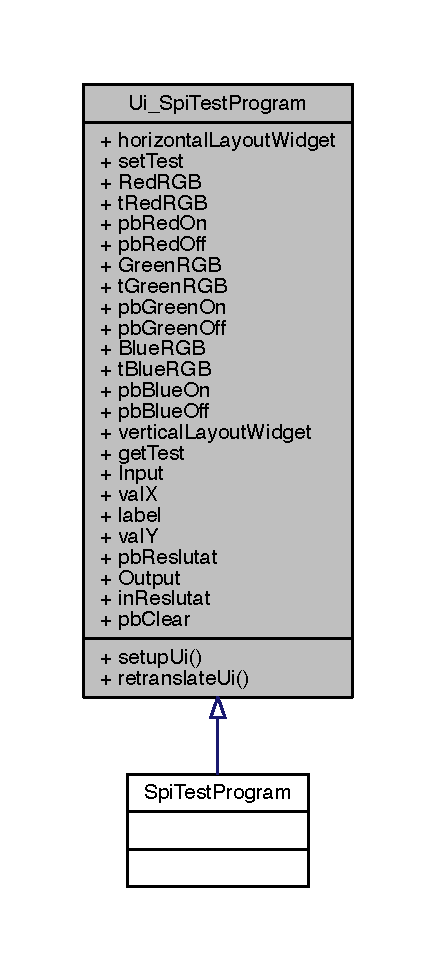
\includegraphics[width=209pt]{d3/dcb/class_ui___spi_test_program__inherit__graph}
\end{center}
\end{figure}


Samarbejdsdiagram for Ui\+\_\+\+Spi\+Test\+Program\+:
\nopagebreak
\begin{figure}[H]
\begin{center}
\leavevmode
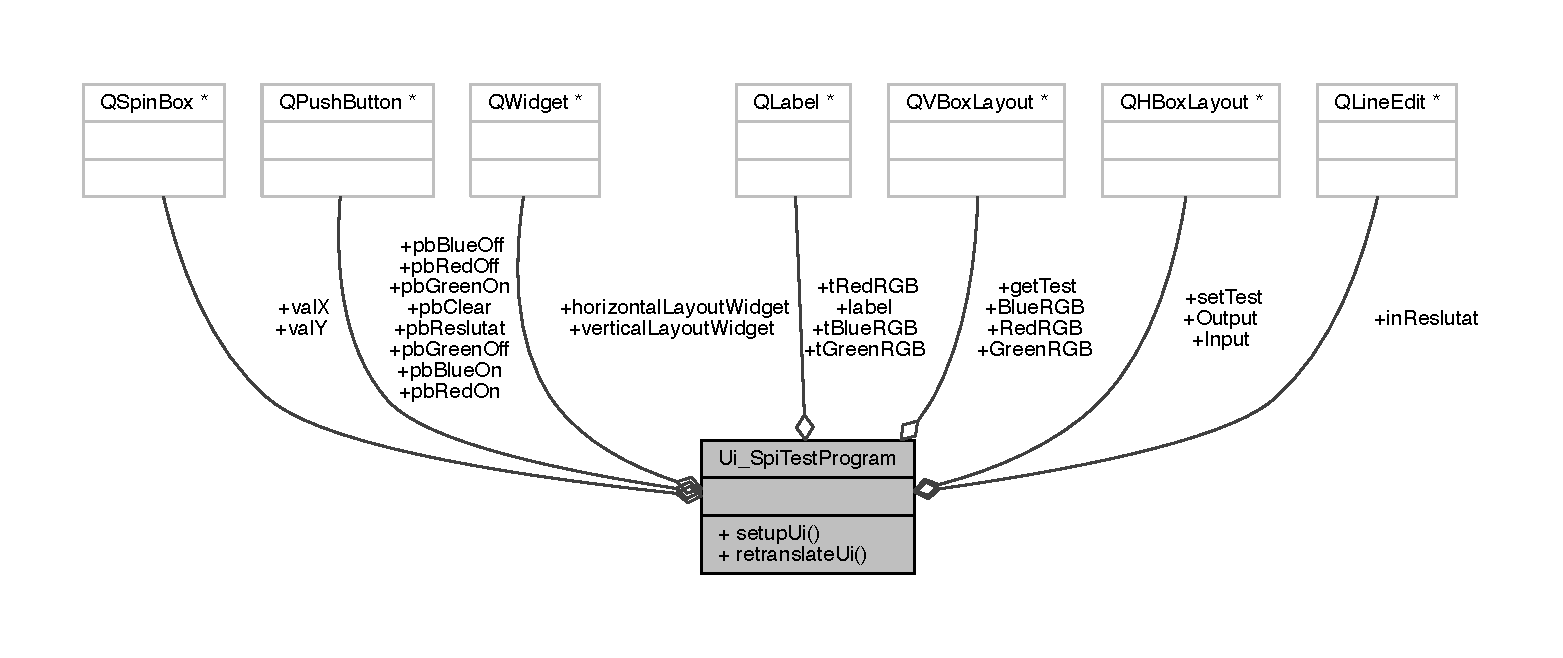
\includegraphics[width=350pt]{d7/d07/class_ui___spi_test_program__coll__graph}
\end{center}
\end{figure}
\subsubsection*{Offentlige metoder}
\begin{DoxyCompactItemize}
\item 
void \hyperlink{class_ui___spi_test_program_a6408f1f402f52e12590b3e4968c84e34}{setup\+Ui} (\hyperlink{class_q_widget}{Q\+Widget} $\ast$\hyperlink{class_spi_test_program}{Spi\+Test\+Program})
\item 
void \hyperlink{class_ui___spi_test_program_a0a1a85fdc36cee52aac338ef3494f996}{retranslate\+Ui} (\hyperlink{class_q_widget}{Q\+Widget} $\ast$\hyperlink{class_spi_test_program}{Spi\+Test\+Program})
\end{DoxyCompactItemize}
\subsubsection*{Datafelter}
\begin{DoxyCompactItemize}
\item 
\hyperlink{class_q_widget}{Q\+Widget} $\ast$ \hyperlink{class_ui___spi_test_program_a8d9662f61dc85ce78495602f1d03006f}{horizontal\+Layout\+Widget}
\item 
Q\+H\+Box\+Layout $\ast$ \hyperlink{class_ui___spi_test_program_ab40f35f9bcce17af63ba573e1e8ee485}{set\+Test}
\item 
Q\+V\+Box\+Layout $\ast$ \hyperlink{class_ui___spi_test_program_a266d140f4ccd88877aee1b242908b21d}{Red\+R\+GB}
\item 
Q\+Label $\ast$ \hyperlink{class_ui___spi_test_program_a44f9277d36451995887541d6e333c772}{t\+Red\+R\+GB}
\item 
Q\+Push\+Button $\ast$ \hyperlink{class_ui___spi_test_program_a58972344360380ab7a3cedec6de9fb0d}{pb\+Red\+On}
\item 
Q\+Push\+Button $\ast$ \hyperlink{class_ui___spi_test_program_ad6661caed9d7154252ff188ea62e538c}{pb\+Red\+Off}
\item 
Q\+V\+Box\+Layout $\ast$ \hyperlink{class_ui___spi_test_program_a45540b28778c355f4e372566eb065ef3}{Green\+R\+GB}
\item 
Q\+Label $\ast$ \hyperlink{class_ui___spi_test_program_a56e39ae0021a6fba651282c09e6d38da}{t\+Green\+R\+GB}
\item 
Q\+Push\+Button $\ast$ \hyperlink{class_ui___spi_test_program_aa00d405e11fadc9dd8d0b7aae2632903}{pb\+Green\+On}
\item 
Q\+Push\+Button $\ast$ \hyperlink{class_ui___spi_test_program_ad4aa6f2ff845832ee96f6158c85bbfba}{pb\+Green\+Off}
\item 
Q\+V\+Box\+Layout $\ast$ \hyperlink{class_ui___spi_test_program_ac0ff6df3d4236129efdc0762eed715f4}{Blue\+R\+GB}
\item 
Q\+Label $\ast$ \hyperlink{class_ui___spi_test_program_a24f37f517fcdcba9802de32d4cb7cd2a}{t\+Blue\+R\+GB}
\item 
Q\+Push\+Button $\ast$ \hyperlink{class_ui___spi_test_program_a3f13697eb9ebac3370cf5b1456bb2ab6}{pb\+Blue\+On}
\item 
Q\+Push\+Button $\ast$ \hyperlink{class_ui___spi_test_program_add50c8a20a19c966af33418b767fb815}{pb\+Blue\+Off}
\item 
\hyperlink{class_q_widget}{Q\+Widget} $\ast$ \hyperlink{class_ui___spi_test_program_a4dab2ee47678bbea22fe10267a009293}{vertical\+Layout\+Widget}
\item 
Q\+V\+Box\+Layout $\ast$ \hyperlink{class_ui___spi_test_program_a6d63969ee767e7e499a5c6abd4424553}{get\+Test}
\item 
Q\+H\+Box\+Layout $\ast$ \hyperlink{class_ui___spi_test_program_a69c0d851a1ffb0301d02c43531ba2f6d}{Input}
\item 
Q\+Spin\+Box $\ast$ \hyperlink{class_ui___spi_test_program_a54b0fe6bef639246ec21b3109185814a}{valX}
\item 
Q\+Label $\ast$ \hyperlink{class_ui___spi_test_program_a22925632964060df176ccbc0de5fa511}{label}
\item 
Q\+Spin\+Box $\ast$ \hyperlink{class_ui___spi_test_program_a88a3fae2c7f772ec60bc66742e8c097e}{valY}
\item 
Q\+Push\+Button $\ast$ \hyperlink{class_ui___spi_test_program_ac3e098e270e17081064d010d68e7f0fc}{pb\+Reslutat}
\item 
Q\+H\+Box\+Layout $\ast$ \hyperlink{class_ui___spi_test_program_a535084bb7ec3f177d317c38db7e93aa6}{Output}
\item 
Q\+Line\+Edit $\ast$ \hyperlink{class_ui___spi_test_program_a14fdf98633693052d40f7b3dfaa64149}{in\+Reslutat}
\item 
Q\+Push\+Button $\ast$ \hyperlink{class_ui___spi_test_program_a9fa60ac8492007635b4648a0c6c88201}{pb\+Clear}
\end{DoxyCompactItemize}


\subsubsection{Detaljeret beskrivelse}


Defineret på linje 27 i filen ui\+\_\+spitestprogram.\+h.



\subsubsection{Dokumentation af medlemsfunktioner}
\index{Ui\+\_\+\+Spi\+Test\+Program@{Ui\+\_\+\+Spi\+Test\+Program}!retranslate\+Ui@{retranslate\+Ui}}
\index{retranslate\+Ui@{retranslate\+Ui}!Ui\+\_\+\+Spi\+Test\+Program@{Ui\+\_\+\+Spi\+Test\+Program}}
\paragraph[{\texorpdfstring{retranslate\+Ui(\+Q\+Widget $\ast$\+Spi\+Test\+Program)}{retranslateUi(QWidget *SpiTestProgram)}}]{\setlength{\rightskip}{0pt plus 5cm}void retranslate\+Ui (
\begin{DoxyParamCaption}
\item[{{\bf Q\+Widget} $\ast$}]{Spi\+Test\+Program}
\end{DoxyParamCaption}
)\hspace{0.3cm}{\ttfamily [inline]}}\hypertarget{class_ui___spi_test_program_a0a1a85fdc36cee52aac338ef3494f996}{}\label{class_ui___spi_test_program_a0a1a85fdc36cee52aac338ef3494f996}


Defineret på linje 214 i filen ui\+\_\+spitestprogram.\+h.



Refereret til af setup\+Ui().


\begin{DoxyCode}
215     \{
216         \hyperlink{class_ui___spi_test_program_a44f9277d36451995887541d6e333c772}{tRedRGB}->setText(QApplication::translate(\textcolor{stringliteral}{"SpiTestProgram"}, \textcolor{stringliteral}{"Red RGB"}, 0, 
      QApplication::UnicodeUTF8));
217         \hyperlink{class_ui___spi_test_program_a58972344360380ab7a3cedec6de9fb0d}{pbRedOn}->setText(QApplication::translate(\textcolor{stringliteral}{"SpiTestProgram"}, \textcolor{stringliteral}{"On"}, 0, 
      QApplication::UnicodeUTF8));
218         \hyperlink{class_ui___spi_test_program_ad6661caed9d7154252ff188ea62e538c}{pbRedOff}->setText(QApplication::translate(\textcolor{stringliteral}{"SpiTestProgram"}, \textcolor{stringliteral}{"Off"}, 0, 
      QApplication::UnicodeUTF8));
219         \hyperlink{class_ui___spi_test_program_a56e39ae0021a6fba651282c09e6d38da}{tGreenRGB}->setText(QApplication::translate(\textcolor{stringliteral}{"SpiTestProgram"}, \textcolor{stringliteral}{"Green RGB"}, 0, 
      QApplication::UnicodeUTF8));
220         \hyperlink{class_ui___spi_test_program_aa00d405e11fadc9dd8d0b7aae2632903}{pbGreenOn}->setText(QApplication::translate(\textcolor{stringliteral}{"SpiTestProgram"}, \textcolor{stringliteral}{"On"}, 0, 
      QApplication::UnicodeUTF8));
221         \hyperlink{class_ui___spi_test_program_ad4aa6f2ff845832ee96f6158c85bbfba}{pbGreenOff}->setText(QApplication::translate(\textcolor{stringliteral}{"SpiTestProgram"}, \textcolor{stringliteral}{"Off"}, 0, 
      QApplication::UnicodeUTF8));
222         \hyperlink{class_ui___spi_test_program_a24f37f517fcdcba9802de32d4cb7cd2a}{tBlueRGB}->setText(QApplication::translate(\textcolor{stringliteral}{"SpiTestProgram"}, \textcolor{stringliteral}{"Blue RGB"}, 0, 
      QApplication::UnicodeUTF8));
223         \hyperlink{class_ui___spi_test_program_a3f13697eb9ebac3370cf5b1456bb2ab6}{pbBlueOn}->setText(QApplication::translate(\textcolor{stringliteral}{"SpiTestProgram"}, \textcolor{stringliteral}{"On"}, 0, 
      QApplication::UnicodeUTF8));
224         \hyperlink{class_ui___spi_test_program_add50c8a20a19c966af33418b767fb815}{pbBlueOff}->setText(QApplication::translate(\textcolor{stringliteral}{"SpiTestProgram"}, \textcolor{stringliteral}{"Off"}, 0, 
      QApplication::UnicodeUTF8));
225         \hyperlink{class_ui___spi_test_program_a22925632964060df176ccbc0de5fa511}{label}->setText(QApplication::translate(\textcolor{stringliteral}{"SpiTestProgram"}, \textcolor{stringliteral}{"x"}, 0, QApplication::UnicodeUTF8));
226         \hyperlink{class_ui___spi_test_program_ac3e098e270e17081064d010d68e7f0fc}{pbReslutat}->setText(QApplication::translate(\textcolor{stringliteral}{"SpiTestProgram"}, \textcolor{stringliteral}{"Resultat"}, 0, 
      QApplication::UnicodeUTF8));
227         \hyperlink{class_ui___spi_test_program_a9fa60ac8492007635b4648a0c6c88201}{pbClear}->setText(QApplication::translate(\textcolor{stringliteral}{"SpiTestProgram"}, \textcolor{stringliteral}{"Clear"}, 0, 
      QApplication::UnicodeUTF8));
228         Q\_UNUSED(SpiTestProgram);
229     \} \textcolor{comment}{// retranslateUi}
\end{DoxyCode}


Her er kalder-\/grafen for denne funktion\+:
\nopagebreak
\begin{figure}[H]
\begin{center}
\leavevmode
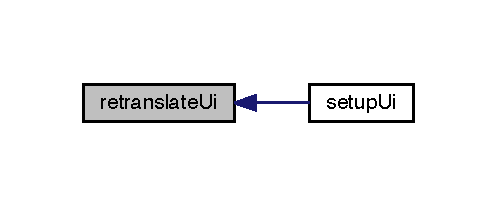
\includegraphics[width=239pt]{d7/de1/class_ui___spi_test_program_a0a1a85fdc36cee52aac338ef3494f996_icgraph}
\end{center}
\end{figure}


\index{Ui\+\_\+\+Spi\+Test\+Program@{Ui\+\_\+\+Spi\+Test\+Program}!setup\+Ui@{setup\+Ui}}
\index{setup\+Ui@{setup\+Ui}!Ui\+\_\+\+Spi\+Test\+Program@{Ui\+\_\+\+Spi\+Test\+Program}}
\paragraph[{\texorpdfstring{setup\+Ui(\+Q\+Widget $\ast$\+Spi\+Test\+Program)}{setupUi(QWidget *SpiTestProgram)}}]{\setlength{\rightskip}{0pt plus 5cm}void setup\+Ui (
\begin{DoxyParamCaption}
\item[{{\bf Q\+Widget} $\ast$}]{Spi\+Test\+Program}
\end{DoxyParamCaption}
)\hspace{0.3cm}{\ttfamily [inline]}}\hypertarget{class_ui___spi_test_program_a6408f1f402f52e12590b3e4968c84e34}{}\label{class_ui___spi_test_program_a6408f1f402f52e12590b3e4968c84e34}


Defineret på linje 55 i filen ui\+\_\+spitestprogram.\+h.



Indeholder referencer til retranslate\+Ui().


\begin{DoxyCode}
56     \{
57         \textcolor{keywordflow}{if} (SpiTestProgram->objectName().isEmpty())
58             SpiTestProgram->setObjectName(QString::fromUtf8(\textcolor{stringliteral}{"SpiTestProgram"}));
59         SpiTestProgram->resize(480, 272);
60         QSizePolicy sizePolicy(QSizePolicy::Fixed, QSizePolicy::Fixed);
61         sizePolicy.setHorizontalStretch(0);
62         sizePolicy.setVerticalStretch(0);
63         sizePolicy.setHeightForWidth(SpiTestProgram->sizePolicy().hasHeightForWidth());
64         SpiTestProgram->setSizePolicy(sizePolicy);
65         SpiTestProgram->setMinimumSize(QSize(480, 272));
66         SpiTestProgram->setMaximumSize(QSize(480, 272));
67         \hyperlink{class_ui___spi_test_program_a8d9662f61dc85ce78495602f1d03006f}{horizontalLayoutWidget} = \textcolor{keyword}{new} \hyperlink{class_q_widget}{QWidget}(SpiTestProgram);
68         \hyperlink{class_ui___spi_test_program_a8d9662f61dc85ce78495602f1d03006f}{horizontalLayoutWidget}->setObjectName(QString::fromUtf8(\textcolor{stringliteral}{"
      horizontalLayoutWidget"}));
69         \hyperlink{class_ui___spi_test_program_a8d9662f61dc85ce78495602f1d03006f}{horizontalLayoutWidget}->setGeometry(QRect(9, 9, 461, 131));
70         \hyperlink{class_ui___spi_test_program_ab40f35f9bcce17af63ba573e1e8ee485}{setTest} = \textcolor{keyword}{new} QHBoxLayout(\hyperlink{class_ui___spi_test_program_a8d9662f61dc85ce78495602f1d03006f}{horizontalLayoutWidget});
71         \hyperlink{class_ui___spi_test_program_ab40f35f9bcce17af63ba573e1e8ee485}{setTest}->setSpacing(6);
72         \hyperlink{class_ui___spi_test_program_ab40f35f9bcce17af63ba573e1e8ee485}{setTest}->setContentsMargins(11, 11, 11, 11);
73         \hyperlink{class_ui___spi_test_program_ab40f35f9bcce17af63ba573e1e8ee485}{setTest}->setObjectName(QString::fromUtf8(\textcolor{stringliteral}{"setTest"}));
74         \hyperlink{class_ui___spi_test_program_ab40f35f9bcce17af63ba573e1e8ee485}{setTest}->setContentsMargins(0, 0, 0, 0);
75         \hyperlink{class_ui___spi_test_program_a266d140f4ccd88877aee1b242908b21d}{RedRGB} = \textcolor{keyword}{new} QVBoxLayout();
76         \hyperlink{class_ui___spi_test_program_a266d140f4ccd88877aee1b242908b21d}{RedRGB}->setSpacing(6);
77         \hyperlink{class_ui___spi_test_program_a266d140f4ccd88877aee1b242908b21d}{RedRGB}->setObjectName(QString::fromUtf8(\textcolor{stringliteral}{"RedRGB"}));
78         \hyperlink{class_ui___spi_test_program_a44f9277d36451995887541d6e333c772}{tRedRGB} = \textcolor{keyword}{new} QLabel(\hyperlink{class_ui___spi_test_program_a8d9662f61dc85ce78495602f1d03006f}{horizontalLayoutWidget});
79         \hyperlink{class_ui___spi_test_program_a44f9277d36451995887541d6e333c772}{tRedRGB}->setObjectName(QString::fromUtf8(\textcolor{stringliteral}{"tRedRGB"}));
80         \hyperlink{class_ui___spi_test_program_a44f9277d36451995887541d6e333c772}{tRedRGB}->setMaximumSize(QSize(272, 30));
81         \hyperlink{class_ui___spi_test_program_a44f9277d36451995887541d6e333c772}{tRedRGB}->setAlignment(Qt::AlignCenter);
82 
83         \hyperlink{class_ui___spi_test_program_a266d140f4ccd88877aee1b242908b21d}{RedRGB}->addWidget(\hyperlink{class_ui___spi_test_program_a44f9277d36451995887541d6e333c772}{tRedRGB});
84 
85         \hyperlink{class_ui___spi_test_program_a58972344360380ab7a3cedec6de9fb0d}{pbRedOn} = \textcolor{keyword}{new} QPushButton(\hyperlink{class_ui___spi_test_program_a8d9662f61dc85ce78495602f1d03006f}{horizontalLayoutWidget});
86         \hyperlink{class_ui___spi_test_program_a58972344360380ab7a3cedec6de9fb0d}{pbRedOn}->setObjectName(QString::fromUtf8(\textcolor{stringliteral}{"pbRedOn"}));
87         \hyperlink{class_ui___spi_test_program_a58972344360380ab7a3cedec6de9fb0d}{pbRedOn}->setMaximumSize(QSize(160, 30));
88 
89         \hyperlink{class_ui___spi_test_program_a266d140f4ccd88877aee1b242908b21d}{RedRGB}->addWidget(\hyperlink{class_ui___spi_test_program_a58972344360380ab7a3cedec6de9fb0d}{pbRedOn});
90 
91         \hyperlink{class_ui___spi_test_program_ad6661caed9d7154252ff188ea62e538c}{pbRedOff} = \textcolor{keyword}{new} QPushButton(\hyperlink{class_ui___spi_test_program_a8d9662f61dc85ce78495602f1d03006f}{horizontalLayoutWidget});
92         \hyperlink{class_ui___spi_test_program_ad6661caed9d7154252ff188ea62e538c}{pbRedOff}->setObjectName(QString::fromUtf8(\textcolor{stringliteral}{"pbRedOff"}));
93         \hyperlink{class_ui___spi_test_program_ad6661caed9d7154252ff188ea62e538c}{pbRedOff}->setMaximumSize(QSize(160, 30));
94 
95         \hyperlink{class_ui___spi_test_program_a266d140f4ccd88877aee1b242908b21d}{RedRGB}->addWidget(\hyperlink{class_ui___spi_test_program_ad6661caed9d7154252ff188ea62e538c}{pbRedOff});
96 
97 
98         \hyperlink{class_ui___spi_test_program_ab40f35f9bcce17af63ba573e1e8ee485}{setTest}->addLayout(\hyperlink{class_ui___spi_test_program_a266d140f4ccd88877aee1b242908b21d}{RedRGB});
99 
100         \hyperlink{class_ui___spi_test_program_a45540b28778c355f4e372566eb065ef3}{GreenRGB} = \textcolor{keyword}{new} QVBoxLayout();
101         \hyperlink{class_ui___spi_test_program_a45540b28778c355f4e372566eb065ef3}{GreenRGB}->setSpacing(6);
102         \hyperlink{class_ui___spi_test_program_a45540b28778c355f4e372566eb065ef3}{GreenRGB}->setObjectName(QString::fromUtf8(\textcolor{stringliteral}{"GreenRGB"}));
103         \hyperlink{class_ui___spi_test_program_a56e39ae0021a6fba651282c09e6d38da}{tGreenRGB} = \textcolor{keyword}{new} QLabel(\hyperlink{class_ui___spi_test_program_a8d9662f61dc85ce78495602f1d03006f}{horizontalLayoutWidget});
104         \hyperlink{class_ui___spi_test_program_a56e39ae0021a6fba651282c09e6d38da}{tGreenRGB}->setObjectName(QString::fromUtf8(\textcolor{stringliteral}{"tGreenRGB"}));
105         \hyperlink{class_ui___spi_test_program_a56e39ae0021a6fba651282c09e6d38da}{tGreenRGB}->setMaximumSize(QSize(160, 30));
106         \hyperlink{class_ui___spi_test_program_a56e39ae0021a6fba651282c09e6d38da}{tGreenRGB}->setAlignment(Qt::AlignCenter);
107 
108         \hyperlink{class_ui___spi_test_program_a45540b28778c355f4e372566eb065ef3}{GreenRGB}->addWidget(\hyperlink{class_ui___spi_test_program_a56e39ae0021a6fba651282c09e6d38da}{tGreenRGB});
109 
110         \hyperlink{class_ui___spi_test_program_aa00d405e11fadc9dd8d0b7aae2632903}{pbGreenOn} = \textcolor{keyword}{new} QPushButton(\hyperlink{class_ui___spi_test_program_a8d9662f61dc85ce78495602f1d03006f}{horizontalLayoutWidget});
111         \hyperlink{class_ui___spi_test_program_aa00d405e11fadc9dd8d0b7aae2632903}{pbGreenOn}->setObjectName(QString::fromUtf8(\textcolor{stringliteral}{"pbGreenOn"}));
112         \hyperlink{class_ui___spi_test_program_aa00d405e11fadc9dd8d0b7aae2632903}{pbGreenOn}->setMaximumSize(QSize(160, 30));
113 
114         \hyperlink{class_ui___spi_test_program_a45540b28778c355f4e372566eb065ef3}{GreenRGB}->addWidget(\hyperlink{class_ui___spi_test_program_aa00d405e11fadc9dd8d0b7aae2632903}{pbGreenOn});
115 
116         \hyperlink{class_ui___spi_test_program_ad4aa6f2ff845832ee96f6158c85bbfba}{pbGreenOff} = \textcolor{keyword}{new} QPushButton(\hyperlink{class_ui___spi_test_program_a8d9662f61dc85ce78495602f1d03006f}{horizontalLayoutWidget});
117         \hyperlink{class_ui___spi_test_program_ad4aa6f2ff845832ee96f6158c85bbfba}{pbGreenOff}->setObjectName(QString::fromUtf8(\textcolor{stringliteral}{"pbGreenOff"}));
118         \hyperlink{class_ui___spi_test_program_ad4aa6f2ff845832ee96f6158c85bbfba}{pbGreenOff}->setMaximumSize(QSize(160, 30));
119 
120         \hyperlink{class_ui___spi_test_program_a45540b28778c355f4e372566eb065ef3}{GreenRGB}->addWidget(\hyperlink{class_ui___spi_test_program_ad4aa6f2ff845832ee96f6158c85bbfba}{pbGreenOff});
121 
122 
123         \hyperlink{class_ui___spi_test_program_ab40f35f9bcce17af63ba573e1e8ee485}{setTest}->addLayout(\hyperlink{class_ui___spi_test_program_a45540b28778c355f4e372566eb065ef3}{GreenRGB});
124 
125         \hyperlink{class_ui___spi_test_program_ac0ff6df3d4236129efdc0762eed715f4}{BlueRGB} = \textcolor{keyword}{new} QVBoxLayout();
126         \hyperlink{class_ui___spi_test_program_ac0ff6df3d4236129efdc0762eed715f4}{BlueRGB}->setSpacing(6);
127         \hyperlink{class_ui___spi_test_program_ac0ff6df3d4236129efdc0762eed715f4}{BlueRGB}->setObjectName(QString::fromUtf8(\textcolor{stringliteral}{"BlueRGB"}));
128         \hyperlink{class_ui___spi_test_program_a24f37f517fcdcba9802de32d4cb7cd2a}{tBlueRGB} = \textcolor{keyword}{new} QLabel(\hyperlink{class_ui___spi_test_program_a8d9662f61dc85ce78495602f1d03006f}{horizontalLayoutWidget});
129         \hyperlink{class_ui___spi_test_program_a24f37f517fcdcba9802de32d4cb7cd2a}{tBlueRGB}->setObjectName(QString::fromUtf8(\textcolor{stringliteral}{"tBlueRGB"}));
130         \hyperlink{class_ui___spi_test_program_a24f37f517fcdcba9802de32d4cb7cd2a}{tBlueRGB}->setMaximumSize(QSize(160, 30));
131         \hyperlink{class_ui___spi_test_program_a24f37f517fcdcba9802de32d4cb7cd2a}{tBlueRGB}->setAlignment(Qt::AlignCenter);
132 
133         \hyperlink{class_ui___spi_test_program_ac0ff6df3d4236129efdc0762eed715f4}{BlueRGB}->addWidget(\hyperlink{class_ui___spi_test_program_a24f37f517fcdcba9802de32d4cb7cd2a}{tBlueRGB});
134 
135         \hyperlink{class_ui___spi_test_program_a3f13697eb9ebac3370cf5b1456bb2ab6}{pbBlueOn} = \textcolor{keyword}{new} QPushButton(\hyperlink{class_ui___spi_test_program_a8d9662f61dc85ce78495602f1d03006f}{horizontalLayoutWidget});
136         \hyperlink{class_ui___spi_test_program_a3f13697eb9ebac3370cf5b1456bb2ab6}{pbBlueOn}->setObjectName(QString::fromUtf8(\textcolor{stringliteral}{"pbBlueOn"}));
137         \hyperlink{class_ui___spi_test_program_a3f13697eb9ebac3370cf5b1456bb2ab6}{pbBlueOn}->setMaximumSize(QSize(160, 30));
138 
139         \hyperlink{class_ui___spi_test_program_ac0ff6df3d4236129efdc0762eed715f4}{BlueRGB}->addWidget(\hyperlink{class_ui___spi_test_program_a3f13697eb9ebac3370cf5b1456bb2ab6}{pbBlueOn});
140 
141         \hyperlink{class_ui___spi_test_program_add50c8a20a19c966af33418b767fb815}{pbBlueOff} = \textcolor{keyword}{new} QPushButton(\hyperlink{class_ui___spi_test_program_a8d9662f61dc85ce78495602f1d03006f}{horizontalLayoutWidget});
142         \hyperlink{class_ui___spi_test_program_add50c8a20a19c966af33418b767fb815}{pbBlueOff}->setObjectName(QString::fromUtf8(\textcolor{stringliteral}{"pbBlueOff"}));
143         \hyperlink{class_ui___spi_test_program_add50c8a20a19c966af33418b767fb815}{pbBlueOff}->setMaximumSize(QSize(160, 30));
144 
145         \hyperlink{class_ui___spi_test_program_ac0ff6df3d4236129efdc0762eed715f4}{BlueRGB}->addWidget(\hyperlink{class_ui___spi_test_program_add50c8a20a19c966af33418b767fb815}{pbBlueOff});
146 
147 
148         \hyperlink{class_ui___spi_test_program_ab40f35f9bcce17af63ba573e1e8ee485}{setTest}->addLayout(\hyperlink{class_ui___spi_test_program_ac0ff6df3d4236129efdc0762eed715f4}{BlueRGB});
149 
150         \hyperlink{class_ui___spi_test_program_a4dab2ee47678bbea22fe10267a009293}{verticalLayoutWidget} = \textcolor{keyword}{new} \hyperlink{class_q_widget}{QWidget}(SpiTestProgram);
151         \hyperlink{class_ui___spi_test_program_a4dab2ee47678bbea22fe10267a009293}{verticalLayoutWidget}->setObjectName(QString::fromUtf8(\textcolor{stringliteral}{"verticalLayoutWidget"}));
152         \hyperlink{class_ui___spi_test_program_a4dab2ee47678bbea22fe10267a009293}{verticalLayoutWidget}->setGeometry(QRect(10, 150, 461, 111));
153         \hyperlink{class_ui___spi_test_program_a6d63969ee767e7e499a5c6abd4424553}{getTest} = \textcolor{keyword}{new} QVBoxLayout(\hyperlink{class_ui___spi_test_program_a4dab2ee47678bbea22fe10267a009293}{verticalLayoutWidget});
154         \hyperlink{class_ui___spi_test_program_a6d63969ee767e7e499a5c6abd4424553}{getTest}->setSpacing(6);
155         \hyperlink{class_ui___spi_test_program_a6d63969ee767e7e499a5c6abd4424553}{getTest}->setContentsMargins(11, 11, 11, 11);
156         \hyperlink{class_ui___spi_test_program_a6d63969ee767e7e499a5c6abd4424553}{getTest}->setObjectName(QString::fromUtf8(\textcolor{stringliteral}{"getTest"}));
157         \hyperlink{class_ui___spi_test_program_a6d63969ee767e7e499a5c6abd4424553}{getTest}->setContentsMargins(0, 0, 0, 0);
158         \hyperlink{class_ui___spi_test_program_a69c0d851a1ffb0301d02c43531ba2f6d}{Input} = \textcolor{keyword}{new} QHBoxLayout();
159         \hyperlink{class_ui___spi_test_program_a69c0d851a1ffb0301d02c43531ba2f6d}{Input}->setSpacing(6);
160         \hyperlink{class_ui___spi_test_program_a69c0d851a1ffb0301d02c43531ba2f6d}{Input}->setObjectName(QString::fromUtf8(\textcolor{stringliteral}{"Input"}));
161         \hyperlink{class_ui___spi_test_program_a54b0fe6bef639246ec21b3109185814a}{valX} = \textcolor{keyword}{new} QSpinBox(\hyperlink{class_ui___spi_test_program_a4dab2ee47678bbea22fe10267a009293}{verticalLayoutWidget});
162         \hyperlink{class_ui___spi_test_program_a54b0fe6bef639246ec21b3109185814a}{valX}->setObjectName(QString::fromUtf8(\textcolor{stringliteral}{"valX"}));
163         \hyperlink{class_ui___spi_test_program_a54b0fe6bef639246ec21b3109185814a}{valX}->setMaximumSize(QSize(160, 30));
164 
165         \hyperlink{class_ui___spi_test_program_a69c0d851a1ffb0301d02c43531ba2f6d}{Input}->addWidget(\hyperlink{class_ui___spi_test_program_a54b0fe6bef639246ec21b3109185814a}{valX});
166 
167         \hyperlink{class_ui___spi_test_program_a22925632964060df176ccbc0de5fa511}{label} = \textcolor{keyword}{new} QLabel(\hyperlink{class_ui___spi_test_program_a4dab2ee47678bbea22fe10267a009293}{verticalLayoutWidget});
168         \hyperlink{class_ui___spi_test_program_a22925632964060df176ccbc0de5fa511}{label}->setObjectName(QString::fromUtf8(\textcolor{stringliteral}{"label"}));
169         \hyperlink{class_ui___spi_test_program_a22925632964060df176ccbc0de5fa511}{label}->setMaximumSize(QSize(20, 30));
170         \hyperlink{class_ui___spi_test_program_a22925632964060df176ccbc0de5fa511}{label}->setAlignment(Qt::AlignCenter);
171 
172         \hyperlink{class_ui___spi_test_program_a69c0d851a1ffb0301d02c43531ba2f6d}{Input}->addWidget(\hyperlink{class_ui___spi_test_program_a22925632964060df176ccbc0de5fa511}{label});
173 
174         \hyperlink{class_ui___spi_test_program_a88a3fae2c7f772ec60bc66742e8c097e}{valY} = \textcolor{keyword}{new} QSpinBox(\hyperlink{class_ui___spi_test_program_a4dab2ee47678bbea22fe10267a009293}{verticalLayoutWidget});
175         \hyperlink{class_ui___spi_test_program_a88a3fae2c7f772ec60bc66742e8c097e}{valY}->setObjectName(QString::fromUtf8(\textcolor{stringliteral}{"valY"}));
176         \hyperlink{class_ui___spi_test_program_a88a3fae2c7f772ec60bc66742e8c097e}{valY}->setMaximumSize(QSize(160, 30));
177 
178         \hyperlink{class_ui___spi_test_program_a69c0d851a1ffb0301d02c43531ba2f6d}{Input}->addWidget(\hyperlink{class_ui___spi_test_program_a88a3fae2c7f772ec60bc66742e8c097e}{valY});
179 
180         \hyperlink{class_ui___spi_test_program_ac3e098e270e17081064d010d68e7f0fc}{pbReslutat} = \textcolor{keyword}{new} QPushButton(\hyperlink{class_ui___spi_test_program_a4dab2ee47678bbea22fe10267a009293}{verticalLayoutWidget});
181         \hyperlink{class_ui___spi_test_program_ac3e098e270e17081064d010d68e7f0fc}{pbReslutat}->setObjectName(QString::fromUtf8(\textcolor{stringliteral}{"pbReslutat"}));
182         \hyperlink{class_ui___spi_test_program_ac3e098e270e17081064d010d68e7f0fc}{pbReslutat}->setMaximumSize(QSize(160, 30));
183 
184         \hyperlink{class_ui___spi_test_program_a69c0d851a1ffb0301d02c43531ba2f6d}{Input}->addWidget(\hyperlink{class_ui___spi_test_program_ac3e098e270e17081064d010d68e7f0fc}{pbReslutat});
185 
186 
187         \hyperlink{class_ui___spi_test_program_a6d63969ee767e7e499a5c6abd4424553}{getTest}->addLayout(\hyperlink{class_ui___spi_test_program_a69c0d851a1ffb0301d02c43531ba2f6d}{Input});
188 
189         \hyperlink{class_ui___spi_test_program_a535084bb7ec3f177d317c38db7e93aa6}{Output} = \textcolor{keyword}{new} QHBoxLayout();
190         \hyperlink{class_ui___spi_test_program_a535084bb7ec3f177d317c38db7e93aa6}{Output}->setSpacing(6);
191         \hyperlink{class_ui___spi_test_program_a535084bb7ec3f177d317c38db7e93aa6}{Output}->setObjectName(QString::fromUtf8(\textcolor{stringliteral}{"Output"}));
192         \hyperlink{class_ui___spi_test_program_a14fdf98633693052d40f7b3dfaa64149}{inReslutat} = \textcolor{keyword}{new} QLineEdit(\hyperlink{class_ui___spi_test_program_a4dab2ee47678bbea22fe10267a009293}{verticalLayoutWidget});
193         \hyperlink{class_ui___spi_test_program_a14fdf98633693052d40f7b3dfaa64149}{inReslutat}->setObjectName(QString::fromUtf8(\textcolor{stringliteral}{"inReslutat"}));
194         \hyperlink{class_ui___spi_test_program_a14fdf98633693052d40f7b3dfaa64149}{inReslutat}->setMaximumSize(QSize(340, 30));
195         \hyperlink{class_ui___spi_test_program_a14fdf98633693052d40f7b3dfaa64149}{inReslutat}->setAlignment(Qt::AlignCenter);
196 
197         \hyperlink{class_ui___spi_test_program_a535084bb7ec3f177d317c38db7e93aa6}{Output}->addWidget(\hyperlink{class_ui___spi_test_program_a14fdf98633693052d40f7b3dfaa64149}{inReslutat});
198 
199         \hyperlink{class_ui___spi_test_program_a9fa60ac8492007635b4648a0c6c88201}{pbClear} = \textcolor{keyword}{new} QPushButton(\hyperlink{class_ui___spi_test_program_a4dab2ee47678bbea22fe10267a009293}{verticalLayoutWidget});
200         \hyperlink{class_ui___spi_test_program_a9fa60ac8492007635b4648a0c6c88201}{pbClear}->setObjectName(QString::fromUtf8(\textcolor{stringliteral}{"pbClear"}));
201         \hyperlink{class_ui___spi_test_program_a9fa60ac8492007635b4648a0c6c88201}{pbClear}->setMaximumSize(QSize(160, 30));
202 
203         \hyperlink{class_ui___spi_test_program_a535084bb7ec3f177d317c38db7e93aa6}{Output}->addWidget(\hyperlink{class_ui___spi_test_program_a9fa60ac8492007635b4648a0c6c88201}{pbClear});
204 
205 
206         \hyperlink{class_ui___spi_test_program_a6d63969ee767e7e499a5c6abd4424553}{getTest}->addLayout(\hyperlink{class_ui___spi_test_program_a535084bb7ec3f177d317c38db7e93aa6}{Output});
207 
208 
209         \hyperlink{class_ui___spi_test_program_a0a1a85fdc36cee52aac338ef3494f996}{retranslateUi}(SpiTestProgram);
210 
211         QMetaObject::connectSlotsByName(SpiTestProgram);
212     \} \textcolor{comment}{// setupUi}
\end{DoxyCode}


Her er kald-\/grafen for denne funktion\+:
\nopagebreak
\begin{figure}[H]
\begin{center}
\leavevmode
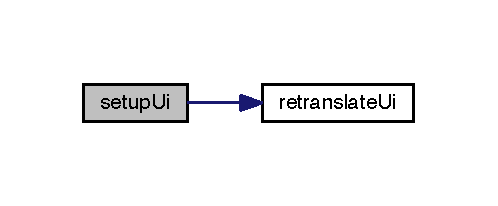
\includegraphics[width=239pt]{d7/de1/class_ui___spi_test_program_a6408f1f402f52e12590b3e4968c84e34_cgraph}
\end{center}
\end{figure}




\subsubsection{Felt-\/dokumentation}
\index{Ui\+\_\+\+Spi\+Test\+Program@{Ui\+\_\+\+Spi\+Test\+Program}!Blue\+R\+GB@{Blue\+R\+GB}}
\index{Blue\+R\+GB@{Blue\+R\+GB}!Ui\+\_\+\+Spi\+Test\+Program@{Ui\+\_\+\+Spi\+Test\+Program}}
\paragraph[{\texorpdfstring{Blue\+R\+GB}{BlueRGB}}]{\setlength{\rightskip}{0pt plus 5cm}Q\+V\+Box\+Layout$\ast$ Blue\+R\+GB}\hypertarget{class_ui___spi_test_program_ac0ff6df3d4236129efdc0762eed715f4}{}\label{class_ui___spi_test_program_ac0ff6df3d4236129efdc0762eed715f4}


Defineret på linje 40 i filen ui\+\_\+spitestprogram.\+h.

\index{Ui\+\_\+\+Spi\+Test\+Program@{Ui\+\_\+\+Spi\+Test\+Program}!get\+Test@{get\+Test}}
\index{get\+Test@{get\+Test}!Ui\+\_\+\+Spi\+Test\+Program@{Ui\+\_\+\+Spi\+Test\+Program}}
\paragraph[{\texorpdfstring{get\+Test}{getTest}}]{\setlength{\rightskip}{0pt plus 5cm}Q\+V\+Box\+Layout$\ast$ get\+Test}\hypertarget{class_ui___spi_test_program_a6d63969ee767e7e499a5c6abd4424553}{}\label{class_ui___spi_test_program_a6d63969ee767e7e499a5c6abd4424553}


Defineret på linje 45 i filen ui\+\_\+spitestprogram.\+h.

\index{Ui\+\_\+\+Spi\+Test\+Program@{Ui\+\_\+\+Spi\+Test\+Program}!Green\+R\+GB@{Green\+R\+GB}}
\index{Green\+R\+GB@{Green\+R\+GB}!Ui\+\_\+\+Spi\+Test\+Program@{Ui\+\_\+\+Spi\+Test\+Program}}
\paragraph[{\texorpdfstring{Green\+R\+GB}{GreenRGB}}]{\setlength{\rightskip}{0pt plus 5cm}Q\+V\+Box\+Layout$\ast$ Green\+R\+GB}\hypertarget{class_ui___spi_test_program_a45540b28778c355f4e372566eb065ef3}{}\label{class_ui___spi_test_program_a45540b28778c355f4e372566eb065ef3}


Defineret på linje 36 i filen ui\+\_\+spitestprogram.\+h.

\index{Ui\+\_\+\+Spi\+Test\+Program@{Ui\+\_\+\+Spi\+Test\+Program}!horizontal\+Layout\+Widget@{horizontal\+Layout\+Widget}}
\index{horizontal\+Layout\+Widget@{horizontal\+Layout\+Widget}!Ui\+\_\+\+Spi\+Test\+Program@{Ui\+\_\+\+Spi\+Test\+Program}}
\paragraph[{\texorpdfstring{horizontal\+Layout\+Widget}{horizontalLayoutWidget}}]{\setlength{\rightskip}{0pt plus 5cm}{\bf Q\+Widget}$\ast$ horizontal\+Layout\+Widget}\hypertarget{class_ui___spi_test_program_a8d9662f61dc85ce78495602f1d03006f}{}\label{class_ui___spi_test_program_a8d9662f61dc85ce78495602f1d03006f}


Defineret på linje 30 i filen ui\+\_\+spitestprogram.\+h.

\index{Ui\+\_\+\+Spi\+Test\+Program@{Ui\+\_\+\+Spi\+Test\+Program}!Input@{Input}}
\index{Input@{Input}!Ui\+\_\+\+Spi\+Test\+Program@{Ui\+\_\+\+Spi\+Test\+Program}}
\paragraph[{\texorpdfstring{Input}{Input}}]{\setlength{\rightskip}{0pt plus 5cm}Q\+H\+Box\+Layout$\ast$ Input}\hypertarget{class_ui___spi_test_program_a69c0d851a1ffb0301d02c43531ba2f6d}{}\label{class_ui___spi_test_program_a69c0d851a1ffb0301d02c43531ba2f6d}


Defineret på linje 46 i filen ui\+\_\+spitestprogram.\+h.

\index{Ui\+\_\+\+Spi\+Test\+Program@{Ui\+\_\+\+Spi\+Test\+Program}!in\+Reslutat@{in\+Reslutat}}
\index{in\+Reslutat@{in\+Reslutat}!Ui\+\_\+\+Spi\+Test\+Program@{Ui\+\_\+\+Spi\+Test\+Program}}
\paragraph[{\texorpdfstring{in\+Reslutat}{inReslutat}}]{\setlength{\rightskip}{0pt plus 5cm}Q\+Line\+Edit$\ast$ in\+Reslutat}\hypertarget{class_ui___spi_test_program_a14fdf98633693052d40f7b3dfaa64149}{}\label{class_ui___spi_test_program_a14fdf98633693052d40f7b3dfaa64149}


Defineret på linje 52 i filen ui\+\_\+spitestprogram.\+h.

\index{Ui\+\_\+\+Spi\+Test\+Program@{Ui\+\_\+\+Spi\+Test\+Program}!label@{label}}
\index{label@{label}!Ui\+\_\+\+Spi\+Test\+Program@{Ui\+\_\+\+Spi\+Test\+Program}}
\paragraph[{\texorpdfstring{label}{label}}]{\setlength{\rightskip}{0pt plus 5cm}Q\+Label$\ast$ label}\hypertarget{class_ui___spi_test_program_a22925632964060df176ccbc0de5fa511}{}\label{class_ui___spi_test_program_a22925632964060df176ccbc0de5fa511}


Defineret på linje 48 i filen ui\+\_\+spitestprogram.\+h.

\index{Ui\+\_\+\+Spi\+Test\+Program@{Ui\+\_\+\+Spi\+Test\+Program}!Output@{Output}}
\index{Output@{Output}!Ui\+\_\+\+Spi\+Test\+Program@{Ui\+\_\+\+Spi\+Test\+Program}}
\paragraph[{\texorpdfstring{Output}{Output}}]{\setlength{\rightskip}{0pt plus 5cm}Q\+H\+Box\+Layout$\ast$ Output}\hypertarget{class_ui___spi_test_program_a535084bb7ec3f177d317c38db7e93aa6}{}\label{class_ui___spi_test_program_a535084bb7ec3f177d317c38db7e93aa6}


Defineret på linje 51 i filen ui\+\_\+spitestprogram.\+h.

\index{Ui\+\_\+\+Spi\+Test\+Program@{Ui\+\_\+\+Spi\+Test\+Program}!pb\+Blue\+Off@{pb\+Blue\+Off}}
\index{pb\+Blue\+Off@{pb\+Blue\+Off}!Ui\+\_\+\+Spi\+Test\+Program@{Ui\+\_\+\+Spi\+Test\+Program}}
\paragraph[{\texorpdfstring{pb\+Blue\+Off}{pbBlueOff}}]{\setlength{\rightskip}{0pt plus 5cm}Q\+Push\+Button$\ast$ pb\+Blue\+Off}\hypertarget{class_ui___spi_test_program_add50c8a20a19c966af33418b767fb815}{}\label{class_ui___spi_test_program_add50c8a20a19c966af33418b767fb815}


Defineret på linje 43 i filen ui\+\_\+spitestprogram.\+h.

\index{Ui\+\_\+\+Spi\+Test\+Program@{Ui\+\_\+\+Spi\+Test\+Program}!pb\+Blue\+On@{pb\+Blue\+On}}
\index{pb\+Blue\+On@{pb\+Blue\+On}!Ui\+\_\+\+Spi\+Test\+Program@{Ui\+\_\+\+Spi\+Test\+Program}}
\paragraph[{\texorpdfstring{pb\+Blue\+On}{pbBlueOn}}]{\setlength{\rightskip}{0pt plus 5cm}Q\+Push\+Button$\ast$ pb\+Blue\+On}\hypertarget{class_ui___spi_test_program_a3f13697eb9ebac3370cf5b1456bb2ab6}{}\label{class_ui___spi_test_program_a3f13697eb9ebac3370cf5b1456bb2ab6}


Defineret på linje 42 i filen ui\+\_\+spitestprogram.\+h.

\index{Ui\+\_\+\+Spi\+Test\+Program@{Ui\+\_\+\+Spi\+Test\+Program}!pb\+Clear@{pb\+Clear}}
\index{pb\+Clear@{pb\+Clear}!Ui\+\_\+\+Spi\+Test\+Program@{Ui\+\_\+\+Spi\+Test\+Program}}
\paragraph[{\texorpdfstring{pb\+Clear}{pbClear}}]{\setlength{\rightskip}{0pt plus 5cm}Q\+Push\+Button$\ast$ pb\+Clear}\hypertarget{class_ui___spi_test_program_a9fa60ac8492007635b4648a0c6c88201}{}\label{class_ui___spi_test_program_a9fa60ac8492007635b4648a0c6c88201}


Defineret på linje 53 i filen ui\+\_\+spitestprogram.\+h.

\index{Ui\+\_\+\+Spi\+Test\+Program@{Ui\+\_\+\+Spi\+Test\+Program}!pb\+Green\+Off@{pb\+Green\+Off}}
\index{pb\+Green\+Off@{pb\+Green\+Off}!Ui\+\_\+\+Spi\+Test\+Program@{Ui\+\_\+\+Spi\+Test\+Program}}
\paragraph[{\texorpdfstring{pb\+Green\+Off}{pbGreenOff}}]{\setlength{\rightskip}{0pt plus 5cm}Q\+Push\+Button$\ast$ pb\+Green\+Off}\hypertarget{class_ui___spi_test_program_ad4aa6f2ff845832ee96f6158c85bbfba}{}\label{class_ui___spi_test_program_ad4aa6f2ff845832ee96f6158c85bbfba}


Defineret på linje 39 i filen ui\+\_\+spitestprogram.\+h.

\index{Ui\+\_\+\+Spi\+Test\+Program@{Ui\+\_\+\+Spi\+Test\+Program}!pb\+Green\+On@{pb\+Green\+On}}
\index{pb\+Green\+On@{pb\+Green\+On}!Ui\+\_\+\+Spi\+Test\+Program@{Ui\+\_\+\+Spi\+Test\+Program}}
\paragraph[{\texorpdfstring{pb\+Green\+On}{pbGreenOn}}]{\setlength{\rightskip}{0pt plus 5cm}Q\+Push\+Button$\ast$ pb\+Green\+On}\hypertarget{class_ui___spi_test_program_aa00d405e11fadc9dd8d0b7aae2632903}{}\label{class_ui___spi_test_program_aa00d405e11fadc9dd8d0b7aae2632903}


Defineret på linje 38 i filen ui\+\_\+spitestprogram.\+h.

\index{Ui\+\_\+\+Spi\+Test\+Program@{Ui\+\_\+\+Spi\+Test\+Program}!pb\+Red\+Off@{pb\+Red\+Off}}
\index{pb\+Red\+Off@{pb\+Red\+Off}!Ui\+\_\+\+Spi\+Test\+Program@{Ui\+\_\+\+Spi\+Test\+Program}}
\paragraph[{\texorpdfstring{pb\+Red\+Off}{pbRedOff}}]{\setlength{\rightskip}{0pt plus 5cm}Q\+Push\+Button$\ast$ pb\+Red\+Off}\hypertarget{class_ui___spi_test_program_ad6661caed9d7154252ff188ea62e538c}{}\label{class_ui___spi_test_program_ad6661caed9d7154252ff188ea62e538c}


Defineret på linje 35 i filen ui\+\_\+spitestprogram.\+h.

\index{Ui\+\_\+\+Spi\+Test\+Program@{Ui\+\_\+\+Spi\+Test\+Program}!pb\+Red\+On@{pb\+Red\+On}}
\index{pb\+Red\+On@{pb\+Red\+On}!Ui\+\_\+\+Spi\+Test\+Program@{Ui\+\_\+\+Spi\+Test\+Program}}
\paragraph[{\texorpdfstring{pb\+Red\+On}{pbRedOn}}]{\setlength{\rightskip}{0pt plus 5cm}Q\+Push\+Button$\ast$ pb\+Red\+On}\hypertarget{class_ui___spi_test_program_a58972344360380ab7a3cedec6de9fb0d}{}\label{class_ui___spi_test_program_a58972344360380ab7a3cedec6de9fb0d}


Defineret på linje 34 i filen ui\+\_\+spitestprogram.\+h.

\index{Ui\+\_\+\+Spi\+Test\+Program@{Ui\+\_\+\+Spi\+Test\+Program}!pb\+Reslutat@{pb\+Reslutat}}
\index{pb\+Reslutat@{pb\+Reslutat}!Ui\+\_\+\+Spi\+Test\+Program@{Ui\+\_\+\+Spi\+Test\+Program}}
\paragraph[{\texorpdfstring{pb\+Reslutat}{pbReslutat}}]{\setlength{\rightskip}{0pt plus 5cm}Q\+Push\+Button$\ast$ pb\+Reslutat}\hypertarget{class_ui___spi_test_program_ac3e098e270e17081064d010d68e7f0fc}{}\label{class_ui___spi_test_program_ac3e098e270e17081064d010d68e7f0fc}


Defineret på linje 50 i filen ui\+\_\+spitestprogram.\+h.

\index{Ui\+\_\+\+Spi\+Test\+Program@{Ui\+\_\+\+Spi\+Test\+Program}!Red\+R\+GB@{Red\+R\+GB}}
\index{Red\+R\+GB@{Red\+R\+GB}!Ui\+\_\+\+Spi\+Test\+Program@{Ui\+\_\+\+Spi\+Test\+Program}}
\paragraph[{\texorpdfstring{Red\+R\+GB}{RedRGB}}]{\setlength{\rightskip}{0pt plus 5cm}Q\+V\+Box\+Layout$\ast$ Red\+R\+GB}\hypertarget{class_ui___spi_test_program_a266d140f4ccd88877aee1b242908b21d}{}\label{class_ui___spi_test_program_a266d140f4ccd88877aee1b242908b21d}


Defineret på linje 32 i filen ui\+\_\+spitestprogram.\+h.

\index{Ui\+\_\+\+Spi\+Test\+Program@{Ui\+\_\+\+Spi\+Test\+Program}!set\+Test@{set\+Test}}
\index{set\+Test@{set\+Test}!Ui\+\_\+\+Spi\+Test\+Program@{Ui\+\_\+\+Spi\+Test\+Program}}
\paragraph[{\texorpdfstring{set\+Test}{setTest}}]{\setlength{\rightskip}{0pt plus 5cm}Q\+H\+Box\+Layout$\ast$ set\+Test}\hypertarget{class_ui___spi_test_program_ab40f35f9bcce17af63ba573e1e8ee485}{}\label{class_ui___spi_test_program_ab40f35f9bcce17af63ba573e1e8ee485}


Defineret på linje 31 i filen ui\+\_\+spitestprogram.\+h.

\index{Ui\+\_\+\+Spi\+Test\+Program@{Ui\+\_\+\+Spi\+Test\+Program}!t\+Blue\+R\+GB@{t\+Blue\+R\+GB}}
\index{t\+Blue\+R\+GB@{t\+Blue\+R\+GB}!Ui\+\_\+\+Spi\+Test\+Program@{Ui\+\_\+\+Spi\+Test\+Program}}
\paragraph[{\texorpdfstring{t\+Blue\+R\+GB}{tBlueRGB}}]{\setlength{\rightskip}{0pt plus 5cm}Q\+Label$\ast$ t\+Blue\+R\+GB}\hypertarget{class_ui___spi_test_program_a24f37f517fcdcba9802de32d4cb7cd2a}{}\label{class_ui___spi_test_program_a24f37f517fcdcba9802de32d4cb7cd2a}


Defineret på linje 41 i filen ui\+\_\+spitestprogram.\+h.

\index{Ui\+\_\+\+Spi\+Test\+Program@{Ui\+\_\+\+Spi\+Test\+Program}!t\+Green\+R\+GB@{t\+Green\+R\+GB}}
\index{t\+Green\+R\+GB@{t\+Green\+R\+GB}!Ui\+\_\+\+Spi\+Test\+Program@{Ui\+\_\+\+Spi\+Test\+Program}}
\paragraph[{\texorpdfstring{t\+Green\+R\+GB}{tGreenRGB}}]{\setlength{\rightskip}{0pt plus 5cm}Q\+Label$\ast$ t\+Green\+R\+GB}\hypertarget{class_ui___spi_test_program_a56e39ae0021a6fba651282c09e6d38da}{}\label{class_ui___spi_test_program_a56e39ae0021a6fba651282c09e6d38da}


Defineret på linje 37 i filen ui\+\_\+spitestprogram.\+h.

\index{Ui\+\_\+\+Spi\+Test\+Program@{Ui\+\_\+\+Spi\+Test\+Program}!t\+Red\+R\+GB@{t\+Red\+R\+GB}}
\index{t\+Red\+R\+GB@{t\+Red\+R\+GB}!Ui\+\_\+\+Spi\+Test\+Program@{Ui\+\_\+\+Spi\+Test\+Program}}
\paragraph[{\texorpdfstring{t\+Red\+R\+GB}{tRedRGB}}]{\setlength{\rightskip}{0pt plus 5cm}Q\+Label$\ast$ t\+Red\+R\+GB}\hypertarget{class_ui___spi_test_program_a44f9277d36451995887541d6e333c772}{}\label{class_ui___spi_test_program_a44f9277d36451995887541d6e333c772}


Defineret på linje 33 i filen ui\+\_\+spitestprogram.\+h.

\index{Ui\+\_\+\+Spi\+Test\+Program@{Ui\+\_\+\+Spi\+Test\+Program}!valX@{valX}}
\index{valX@{valX}!Ui\+\_\+\+Spi\+Test\+Program@{Ui\+\_\+\+Spi\+Test\+Program}}
\paragraph[{\texorpdfstring{valX}{valX}}]{\setlength{\rightskip}{0pt plus 5cm}Q\+Spin\+Box$\ast$ valX}\hypertarget{class_ui___spi_test_program_a54b0fe6bef639246ec21b3109185814a}{}\label{class_ui___spi_test_program_a54b0fe6bef639246ec21b3109185814a}


Defineret på linje 47 i filen ui\+\_\+spitestprogram.\+h.

\index{Ui\+\_\+\+Spi\+Test\+Program@{Ui\+\_\+\+Spi\+Test\+Program}!valY@{valY}}
\index{valY@{valY}!Ui\+\_\+\+Spi\+Test\+Program@{Ui\+\_\+\+Spi\+Test\+Program}}
\paragraph[{\texorpdfstring{valY}{valY}}]{\setlength{\rightskip}{0pt plus 5cm}Q\+Spin\+Box$\ast$ valY}\hypertarget{class_ui___spi_test_program_a88a3fae2c7f772ec60bc66742e8c097e}{}\label{class_ui___spi_test_program_a88a3fae2c7f772ec60bc66742e8c097e}


Defineret på linje 49 i filen ui\+\_\+spitestprogram.\+h.

\index{Ui\+\_\+\+Spi\+Test\+Program@{Ui\+\_\+\+Spi\+Test\+Program}!vertical\+Layout\+Widget@{vertical\+Layout\+Widget}}
\index{vertical\+Layout\+Widget@{vertical\+Layout\+Widget}!Ui\+\_\+\+Spi\+Test\+Program@{Ui\+\_\+\+Spi\+Test\+Program}}
\paragraph[{\texorpdfstring{vertical\+Layout\+Widget}{verticalLayoutWidget}}]{\setlength{\rightskip}{0pt plus 5cm}{\bf Q\+Widget}$\ast$ vertical\+Layout\+Widget}\hypertarget{class_ui___spi_test_program_a4dab2ee47678bbea22fe10267a009293}{}\label{class_ui___spi_test_program_a4dab2ee47678bbea22fe10267a009293}


Defineret på linje 44 i filen ui\+\_\+spitestprogram.\+h.



Dokumentationen for denne klasse blev genereret ud fra filen\+:\begin{DoxyCompactItemize}
\item 
\hyperlink{ui__spitestprogram_8h}{ui\+\_\+spitestprogram.\+h}\end{DoxyCompactItemize}

\section{Fil-\/dokumentation}
\hypertarget{e3pjr_8h}{}\subsection{e3pjr.\+h filreference}
\label{e3pjr_8h}\index{e3pjr.\+h@{e3pjr.\+h}}
{\ttfamily \#include $<$Q\+Tab\+Widget$>$}\\*
{\ttfamily \#include $<$Q\+String$>$}\\*
{\ttfamily \#include $<$Q\+Shortcut\+Event$>$}\\*
{\ttfamily \#include $<$Q\+Key\+Event$>$}\\*
{\ttfamily \#include $<$Q\+Line\+Edit$>$}\\*
{\ttfamily \#include \char`\"{}spiapi.\+h\char`\"{}}\\*
Inklusions-\/afhængighedsgraf for e3pjr.\+h\+:
\nopagebreak
\begin{figure}[H]
\begin{center}
\leavevmode
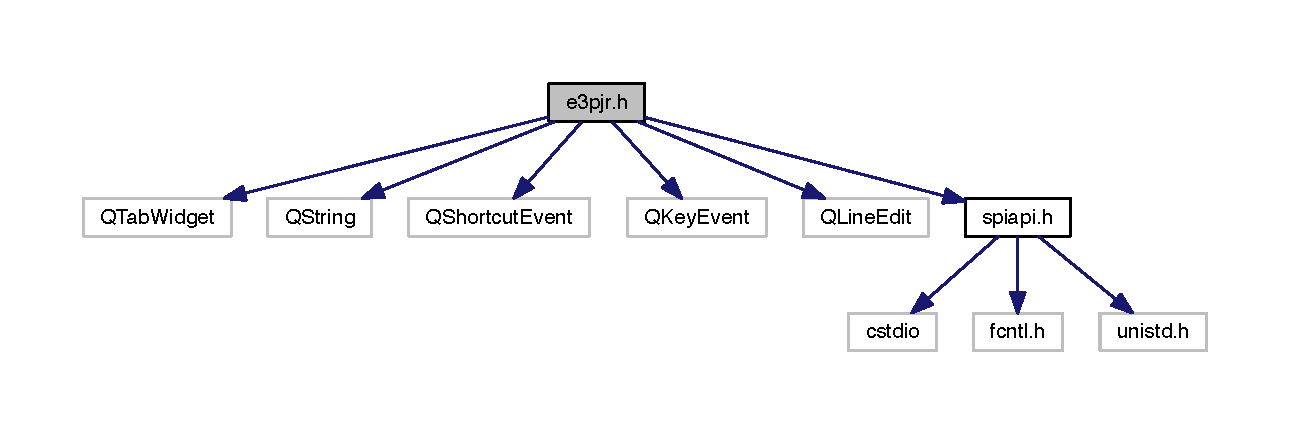
\includegraphics[width=350pt]{e3pjr_8h__incl}
\end{center}
\end{figure}
\subsubsection*{Datastrukturer}
\begin{DoxyCompactItemize}
\item 
class \hyperlink{class_e3_p_j_r}{E3\+P\+JR}
\end{DoxyCompactItemize}
\subsubsection*{Namespaces}
\begin{DoxyCompactItemize}
\item 
 \hyperlink{namespace_ui}{Ui}
\end{DoxyCompactItemize}

\hypertarget{hotplug__psoc__spi__device_8c}{}\subsection{hotplug\+\_\+psoc\+\_\+spi\+\_\+device.\+c filreference}
\label{hotplug__psoc__spi__device_8c}\index{hotplug\+\_\+psoc\+\_\+spi\+\_\+device.\+c@{hotplug\+\_\+psoc\+\_\+spi\+\_\+device.\+c}}
{\ttfamily \#include $<$linux/init.\+h$>$}\\*
{\ttfamily \#include $<$linux/module.\+h$>$}\\*
{\ttfamily \#include $<$linux/spi/spi.\+h$>$}\\*
{\ttfamily \#include $<$asm/uaccess.\+h$>$}\\*
{\ttfamily \#include $<$linux/platform\+\_\+data/spi-\/omap2-\/mcspi.\+h$>$}\\*
Inklusions-\/afhængighedsgraf for hotplug\+\_\+psoc\+\_\+spi\+\_\+device.\+c\+:
\nopagebreak
\begin{figure}[H]
\begin{center}
\leavevmode
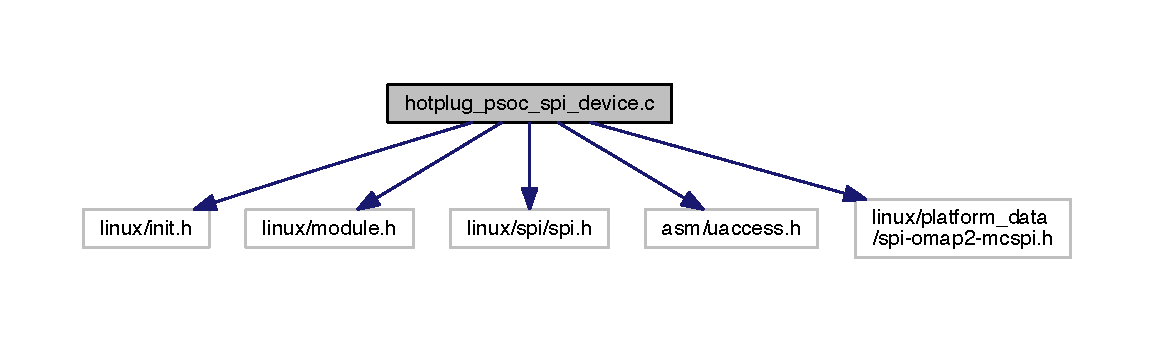
\includegraphics[width=350pt]{d3/dd2/hotplug__psoc__spi__device_8c__incl}
\end{center}
\end{figure}
\subsubsection*{Funktioner}
\begin{DoxyCompactItemize}
\item 
\hyperlink{hotplug__psoc__spi__device_8c_a76205f40e50e793bad85477c56a1fcb5}{M\+O\+D\+U\+L\+E\+\_\+\+A\+U\+T\+H\+OR} (\char`\"{}Jeppe Stærk\char`\"{})
\item 
\hyperlink{hotplug__psoc__spi__device_8c_a5c95e2cd11cba226f5f3513060a8928e}{M\+O\+D\+U\+L\+E\+\_\+\+L\+I\+C\+E\+N\+SE} (\char`\"{}Dual B\+SD/G\+PL\char`\"{})
\item 
static int \hyperlink{hotplug__psoc__spi__device_8c_ad22e734f3f2605901ebaeecc84688362}{hotplug\+\_\+spi\+\_\+init} (void)
\item 
static void \hyperlink{hotplug__psoc__spi__device_8c_aeb21f0923200cce2c073558c826a6257}{hotplug\+\_\+spi\+\_\+exit} (void)
\item 
\hyperlink{hotplug__psoc__spi__device_8c_aa5bc2e887faa7c9d28e378e434228edb}{module\+\_\+init} (\hyperlink{hotplug__psoc__spi__device_8c_ad22e734f3f2605901ebaeecc84688362}{hotplug\+\_\+spi\+\_\+init})
\item 
\hyperlink{hotplug__psoc__spi__device_8c_a9598455ed5fae1360ad263793d9d2357}{module\+\_\+exit} (\hyperlink{hotplug__psoc__spi__device_8c_aeb21f0923200cce2c073558c826a6257}{hotplug\+\_\+spi\+\_\+exit})
\end{DoxyCompactItemize}
\subsubsection*{Variable}
\begin{DoxyCompactItemize}
\item 
static struct spi\+\_\+device $\ast$ \hyperlink{hotplug__psoc__spi__device_8c_a4c80f5a180249a93e8946022ede52199}{slave\+\_\+spi\+\_\+device}
\item 
static struct omap2\+\_\+mcspi\+\_\+device\+\_\+config \hyperlink{hotplug__psoc__spi__device_8c_a52cfe025127b44fa0e131f99a4acfab4}{mcspi\+\_\+config}
\item 
static struct spi\+\_\+board\+\_\+info \hyperlink{hotplug__psoc__spi__device_8c_ae5d3eeebde04f85290320b9f6310b8be}{slave\+\_\+spi\+\_\+board\+\_\+info}
\end{DoxyCompactItemize}


\subsubsection{Funktions-\/dokumentation}
\index{hotplug\+\_\+psoc\+\_\+spi\+\_\+device.\+c@{hotplug\+\_\+psoc\+\_\+spi\+\_\+device.\+c}!hotplug\+\_\+spi\+\_\+exit@{hotplug\+\_\+spi\+\_\+exit}}
\index{hotplug\+\_\+spi\+\_\+exit@{hotplug\+\_\+spi\+\_\+exit}!hotplug\+\_\+psoc\+\_\+spi\+\_\+device.\+c@{hotplug\+\_\+psoc\+\_\+spi\+\_\+device.\+c}}
\paragraph[{\texorpdfstring{hotplug\+\_\+spi\+\_\+exit(void)}{hotplug_spi_exit(void)}}]{\setlength{\rightskip}{0pt plus 5cm}static void hotplug\+\_\+spi\+\_\+exit (
\begin{DoxyParamCaption}
\item[{void}]{}
\end{DoxyParamCaption}
)\hspace{0.3cm}{\ttfamily [static]}}\hypertarget{hotplug__psoc__spi__device_8c_aeb21f0923200cce2c073558c826a6257}{}\label{hotplug__psoc__spi__device_8c_aeb21f0923200cce2c073558c826a6257}


Defineret på linje 67 i filen hotplug\+\_\+psoc\+\_\+spi\+\_\+device.\+c.



Indeholder referencer til hotplug\+\_\+spi\+\_\+init(), module\+\_\+exit(), module\+\_\+init(), slave\+\_\+spi\+\_\+board\+\_\+info og slave\+\_\+spi\+\_\+device.


\begin{DoxyCode}
68 \{
69   printk(KERN\_ALERT \textcolor{stringliteral}{"Removing SPI Device: %s, bus: %i, chip-sel: %i\(\backslash\)n"}, 
70      \hyperlink{hotplug__psoc__spi__device_8c_ae5d3eeebde04f85290320b9f6310b8be}{slave\_spi\_board\_info}.modalias, \hyperlink{hotplug__psoc__spi__device_8c_ae5d3eeebde04f85290320b9f6310b8be}{slave\_spi\_board\_info}.bus\_num, 
      \hyperlink{hotplug__psoc__spi__device_8c_ae5d3eeebde04f85290320b9f6310b8be}{slave\_spi\_board\_info}.chip\_select);
71   spi\_unregister\_device(\hyperlink{hotplug__psoc__spi__device_8c_a4c80f5a180249a93e8946022ede52199}{slave\_spi\_device});
72 \}
\end{DoxyCode}


Her er kald-\/grafen for denne funktion\+:
\nopagebreak
\begin{figure}[H]
\begin{center}
\leavevmode
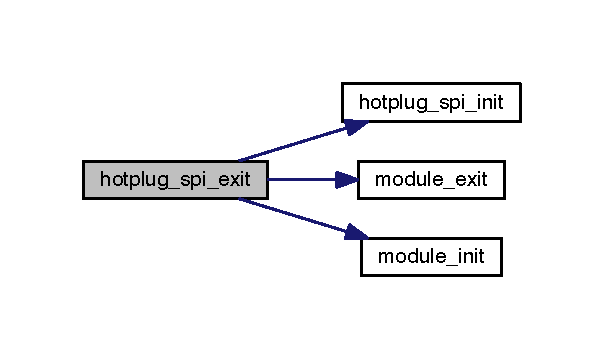
\includegraphics[width=290pt]{d1/dca/hotplug__psoc__spi__device_8c_aeb21f0923200cce2c073558c826a6257_cgraph}
\end{center}
\end{figure}


\index{hotplug\+\_\+psoc\+\_\+spi\+\_\+device.\+c@{hotplug\+\_\+psoc\+\_\+spi\+\_\+device.\+c}!hotplug\+\_\+spi\+\_\+init@{hotplug\+\_\+spi\+\_\+init}}
\index{hotplug\+\_\+spi\+\_\+init@{hotplug\+\_\+spi\+\_\+init}!hotplug\+\_\+psoc\+\_\+spi\+\_\+device.\+c@{hotplug\+\_\+psoc\+\_\+spi\+\_\+device.\+c}}
\paragraph[{\texorpdfstring{hotplug\+\_\+spi\+\_\+init(void)}{hotplug_spi_init(void)}}]{\setlength{\rightskip}{0pt plus 5cm}static int hotplug\+\_\+spi\+\_\+init (
\begin{DoxyParamCaption}
\item[{void}]{}
\end{DoxyParamCaption}
)\hspace{0.3cm}{\ttfamily [static]}}\hypertarget{hotplug__psoc__spi__device_8c_ad22e734f3f2605901ebaeecc84688362}{}\label{hotplug__psoc__spi__device_8c_ad22e734f3f2605901ebaeecc84688362}


Defineret på linje 32 i filen hotplug\+\_\+psoc\+\_\+spi\+\_\+device.\+c.



Indeholder referencer til slave\+\_\+spi\+\_\+board\+\_\+info og slave\+\_\+spi\+\_\+device.



Refereret til af hotplug\+\_\+spi\+\_\+exit().


\begin{DoxyCode}
33 \{
34   \textcolor{keywordtype}{int} bus\_num;
35   \textcolor{keyword}{struct }spi\_master *slaves\_spi\_master;
36 
37   printk(KERN\_ALERT \textcolor{stringliteral}{"Adding SPI Device: %s, bus: %i, chip-sel: %i\(\backslash\)n"}, 
38      \hyperlink{hotplug__psoc__spi__device_8c_ae5d3eeebde04f85290320b9f6310b8be}{slave\_spi\_board\_info}.modalias, \hyperlink{hotplug__psoc__spi__device_8c_ae5d3eeebde04f85290320b9f6310b8be}{slave\_spi\_board\_info}.bus\_num, 
      \hyperlink{hotplug__psoc__spi__device_8c_ae5d3eeebde04f85290320b9f6310b8be}{slave\_spi\_board\_info}.chip\_select);
39   
40   \textcolor{comment}{/* Add the slave SPI device to the SPI bus}
41 \textcolor{comment}{   *}
42 \textcolor{comment}{   * These methods are used to hot-plug spi devices.}
43 \textcolor{comment}{   * SPI devices are by nature NOT hot-pluggable, as}
44 \textcolor{comment}{   * they cannot be probed for functionality etc. SPI}
45 \textcolor{comment}{   * devices are normally cold-plugged during boot, that}
46 \textcolor{comment}{   * is, they are added in the board description file:}
47 \textcolor{comment}{   * /arch/arm/mach-omap2/board-devkit8000.c}
48 \textcolor{comment}{   * Using this method we actually doing "hot" cold-plugging}
49 \textcolor{comment}{   * adding devices using a kernel module.}
50 \textcolor{comment}{   * Note that it is crusial that driver and device uses}
51 \textcolor{comment}{   * the same name alias. If not, the device and driver}
52 \textcolor{comment}{   * will not be paired and the probe method in the driver}
53 \textcolor{comment}{   * not be called.}
54 \textcolor{comment}{   */} 
55   bus\_num = \hyperlink{hotplug__psoc__spi__device_8c_ae5d3eeebde04f85290320b9f6310b8be}{slave\_spi\_board\_info}.bus\_num;
56   slaves\_spi\_master = spi\_busnum\_to\_master(bus\_num);
57   \hyperlink{hotplug__psoc__spi__device_8c_a4c80f5a180249a93e8946022ede52199}{slave\_spi\_device} = spi\_new\_device(slaves\_spi\_master,
58                     &\hyperlink{hotplug__psoc__spi__device_8c_ae5d3eeebde04f85290320b9f6310b8be}{slave\_spi\_board\_info});
59   \textcolor{keywordflow}{if}(\hyperlink{hotplug__psoc__spi__device_8c_a4c80f5a180249a93e8946022ede52199}{slave\_spi\_device} < 0) \{
60     printk(KERN\_ALERT \textcolor{stringliteral}{"Unsuccesful creating a new device\(\backslash\)n"});
61     \textcolor{keywordflow}{return} -1;
62   \}
63     
64   \textcolor{keywordflow}{return} 0;
65 \}
\end{DoxyCode}


Her er kalder-\/grafen for denne funktion\+:
\nopagebreak
\begin{figure}[H]
\begin{center}
\leavevmode
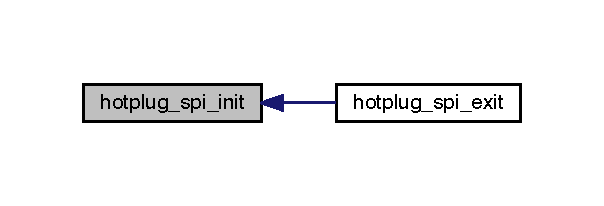
\includegraphics[width=290pt]{d1/dca/hotplug__psoc__spi__device_8c_ad22e734f3f2605901ebaeecc84688362_icgraph}
\end{center}
\end{figure}


\index{hotplug\+\_\+psoc\+\_\+spi\+\_\+device.\+c@{hotplug\+\_\+psoc\+\_\+spi\+\_\+device.\+c}!M\+O\+D\+U\+L\+E\+\_\+\+A\+U\+T\+H\+OR@{M\+O\+D\+U\+L\+E\+\_\+\+A\+U\+T\+H\+OR}}
\index{M\+O\+D\+U\+L\+E\+\_\+\+A\+U\+T\+H\+OR@{M\+O\+D\+U\+L\+E\+\_\+\+A\+U\+T\+H\+OR}!hotplug\+\_\+psoc\+\_\+spi\+\_\+device.\+c@{hotplug\+\_\+psoc\+\_\+spi\+\_\+device.\+c}}
\paragraph[{\texorpdfstring{M\+O\+D\+U\+L\+E\+\_\+\+A\+U\+T\+H\+O\+R(""Jeppe Stærk"")}{MODULE_AUTHOR("Jeppe Stærk")}}]{\setlength{\rightskip}{0pt plus 5cm}M\+O\+D\+U\+L\+E\+\_\+\+A\+U\+T\+H\+OR (
\begin{DoxyParamCaption}
\item[{\char`\"{}Jeppe Stærk\char`\"{}}]{}
\end{DoxyParamCaption}
)}\hypertarget{hotplug__psoc__spi__device_8c_a76205f40e50e793bad85477c56a1fcb5}{}\label{hotplug__psoc__spi__device_8c_a76205f40e50e793bad85477c56a1fcb5}
\index{hotplug\+\_\+psoc\+\_\+spi\+\_\+device.\+c@{hotplug\+\_\+psoc\+\_\+spi\+\_\+device.\+c}!module\+\_\+exit@{module\+\_\+exit}}
\index{module\+\_\+exit@{module\+\_\+exit}!hotplug\+\_\+psoc\+\_\+spi\+\_\+device.\+c@{hotplug\+\_\+psoc\+\_\+spi\+\_\+device.\+c}}
\paragraph[{\texorpdfstring{module\+\_\+exit(hotplug\+\_\+spi\+\_\+exit)}{module_exit(hotplug_spi_exit)}}]{\setlength{\rightskip}{0pt plus 5cm}module\+\_\+exit (
\begin{DoxyParamCaption}
\item[{{\bf hotplug\+\_\+spi\+\_\+exit}}]{}
\end{DoxyParamCaption}
)}\hypertarget{hotplug__psoc__spi__device_8c_a9598455ed5fae1360ad263793d9d2357}{}\label{hotplug__psoc__spi__device_8c_a9598455ed5fae1360ad263793d9d2357}


Refereret til af hotplug\+\_\+spi\+\_\+exit().



Her er kalder-\/grafen for denne funktion\+:
\nopagebreak
\begin{figure}[H]
\begin{center}
\leavevmode
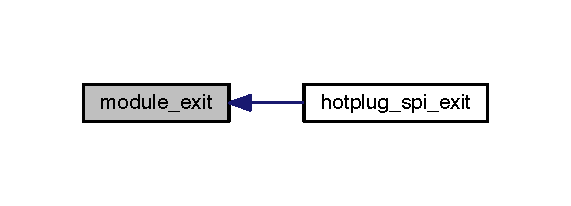
\includegraphics[width=274pt]{d1/dca/hotplug__psoc__spi__device_8c_a9598455ed5fae1360ad263793d9d2357_icgraph}
\end{center}
\end{figure}


\index{hotplug\+\_\+psoc\+\_\+spi\+\_\+device.\+c@{hotplug\+\_\+psoc\+\_\+spi\+\_\+device.\+c}!module\+\_\+init@{module\+\_\+init}}
\index{module\+\_\+init@{module\+\_\+init}!hotplug\+\_\+psoc\+\_\+spi\+\_\+device.\+c@{hotplug\+\_\+psoc\+\_\+spi\+\_\+device.\+c}}
\paragraph[{\texorpdfstring{module\+\_\+init(hotplug\+\_\+spi\+\_\+init)}{module_init(hotplug_spi_init)}}]{\setlength{\rightskip}{0pt plus 5cm}module\+\_\+init (
\begin{DoxyParamCaption}
\item[{{\bf hotplug\+\_\+spi\+\_\+init}}]{}
\end{DoxyParamCaption}
)}\hypertarget{hotplug__psoc__spi__device_8c_aa5bc2e887faa7c9d28e378e434228edb}{}\label{hotplug__psoc__spi__device_8c_aa5bc2e887faa7c9d28e378e434228edb}


Refereret til af hotplug\+\_\+spi\+\_\+exit().



Her er kalder-\/grafen for denne funktion\+:
\nopagebreak
\begin{figure}[H]
\begin{center}
\leavevmode
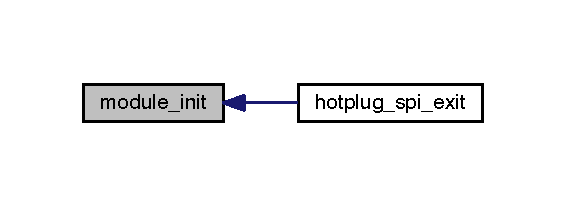
\includegraphics[width=271pt]{d1/dca/hotplug__psoc__spi__device_8c_aa5bc2e887faa7c9d28e378e434228edb_icgraph}
\end{center}
\end{figure}


\index{hotplug\+\_\+psoc\+\_\+spi\+\_\+device.\+c@{hotplug\+\_\+psoc\+\_\+spi\+\_\+device.\+c}!M\+O\+D\+U\+L\+E\+\_\+\+L\+I\+C\+E\+N\+SE@{M\+O\+D\+U\+L\+E\+\_\+\+L\+I\+C\+E\+N\+SE}}
\index{M\+O\+D\+U\+L\+E\+\_\+\+L\+I\+C\+E\+N\+SE@{M\+O\+D\+U\+L\+E\+\_\+\+L\+I\+C\+E\+N\+SE}!hotplug\+\_\+psoc\+\_\+spi\+\_\+device.\+c@{hotplug\+\_\+psoc\+\_\+spi\+\_\+device.\+c}}
\paragraph[{\texorpdfstring{M\+O\+D\+U\+L\+E\+\_\+\+L\+I\+C\+E\+N\+S\+E(""Dual B\+S\+D/\+G\+PL"")}{MODULE_LICENSE("Dual BSD/GPL")}}]{\setlength{\rightskip}{0pt plus 5cm}M\+O\+D\+U\+L\+E\+\_\+\+L\+I\+C\+E\+N\+SE (
\begin{DoxyParamCaption}
\item[{\char`\"{}Dual B\+SD/G\+PL\char`\"{}}]{}
\end{DoxyParamCaption}
)}\hypertarget{hotplug__psoc__spi__device_8c_a5c95e2cd11cba226f5f3513060a8928e}{}\label{hotplug__psoc__spi__device_8c_a5c95e2cd11cba226f5f3513060a8928e}


\subsubsection{Variabel-\/dokumentation}
\index{hotplug\+\_\+psoc\+\_\+spi\+\_\+device.\+c@{hotplug\+\_\+psoc\+\_\+spi\+\_\+device.\+c}!mcspi\+\_\+config@{mcspi\+\_\+config}}
\index{mcspi\+\_\+config@{mcspi\+\_\+config}!hotplug\+\_\+psoc\+\_\+spi\+\_\+device.\+c@{hotplug\+\_\+psoc\+\_\+spi\+\_\+device.\+c}}
\paragraph[{\texorpdfstring{mcspi\+\_\+config}{mcspi_config}}]{\setlength{\rightskip}{0pt plus 5cm}struct omap2\+\_\+mcspi\+\_\+device\+\_\+config mcspi\+\_\+config\hspace{0.3cm}{\ttfamily [static]}}\hypertarget{hotplug__psoc__spi__device_8c_a52cfe025127b44fa0e131f99a4acfab4}{}\label{hotplug__psoc__spi__device_8c_a52cfe025127b44fa0e131f99a4acfab4}
{\bfseries Startværdi\+:}
\begin{DoxyCode}
= \{
  .turbo\_mode       = 1,
\}
\end{DoxyCode}


Defineret på linje 16 i filen hotplug\+\_\+psoc\+\_\+spi\+\_\+device.\+c.

\index{hotplug\+\_\+psoc\+\_\+spi\+\_\+device.\+c@{hotplug\+\_\+psoc\+\_\+spi\+\_\+device.\+c}!slave\+\_\+spi\+\_\+board\+\_\+info@{slave\+\_\+spi\+\_\+board\+\_\+info}}
\index{slave\+\_\+spi\+\_\+board\+\_\+info@{slave\+\_\+spi\+\_\+board\+\_\+info}!hotplug\+\_\+psoc\+\_\+spi\+\_\+device.\+c@{hotplug\+\_\+psoc\+\_\+spi\+\_\+device.\+c}}
\paragraph[{\texorpdfstring{slave\+\_\+spi\+\_\+board\+\_\+info}{slave_spi_board_info}}]{\setlength{\rightskip}{0pt plus 5cm}struct spi\+\_\+board\+\_\+info slave\+\_\+spi\+\_\+board\+\_\+info\hspace{0.3cm}{\ttfamily [static]}}\hypertarget{hotplug__psoc__spi__device_8c_ae5d3eeebde04f85290320b9f6310b8be}{}\label{hotplug__psoc__spi__device_8c_ae5d3eeebde04f85290320b9f6310b8be}
{\bfseries Startværdi\+:}
\begin{DoxyCode}
= \{
  .modalias     = \textcolor{stringliteral}{"psoc4"},
  .bus\_num      = 1,
  .chip\_select      = 0,
  .max\_speed\_hz     = 100000,
  .controller\_data  = &\hyperlink{hotplug__psoc__spi__device_8c_a52cfe025127b44fa0e131f99a4acfab4}{mcspi\_config},
  .mode             = SPI\_MODE\_3, 
\}
\end{DoxyCode}


Defineret på linje 23 i filen hotplug\+\_\+psoc\+\_\+spi\+\_\+device.\+c.



Refereret til af hotplug\+\_\+spi\+\_\+exit() og hotplug\+\_\+spi\+\_\+init().

\index{hotplug\+\_\+psoc\+\_\+spi\+\_\+device.\+c@{hotplug\+\_\+psoc\+\_\+spi\+\_\+device.\+c}!slave\+\_\+spi\+\_\+device@{slave\+\_\+spi\+\_\+device}}
\index{slave\+\_\+spi\+\_\+device@{slave\+\_\+spi\+\_\+device}!hotplug\+\_\+psoc\+\_\+spi\+\_\+device.\+c@{hotplug\+\_\+psoc\+\_\+spi\+\_\+device.\+c}}
\paragraph[{\texorpdfstring{slave\+\_\+spi\+\_\+device}{slave_spi_device}}]{\setlength{\rightskip}{0pt plus 5cm}struct spi\+\_\+device$\ast$ slave\+\_\+spi\+\_\+device\hspace{0.3cm}{\ttfamily [static]}}\hypertarget{hotplug__psoc__spi__device_8c_a4c80f5a180249a93e8946022ede52199}{}\label{hotplug__psoc__spi__device_8c_a4c80f5a180249a93e8946022ede52199}


Defineret på linje 11 i filen hotplug\+\_\+psoc\+\_\+spi\+\_\+device.\+c.



Refereret til af hotplug\+\_\+spi\+\_\+exit() og hotplug\+\_\+spi\+\_\+init().


\hypertarget{light_8h}{}\subsection{light.\+h filreference}
\label{light_8h}\index{light.\+h@{light.\+h}}
{\ttfamily \#include $<$Q\+Widget$>$}\\*
Inklusions-\/afhængighedsgraf for light.\+h\+:\nopagebreak
\begin{figure}[H]
\begin{center}
\leavevmode
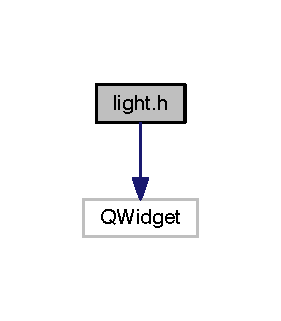
\includegraphics[width=135pt]{d5/dfc/light_8h__incl}
\end{center}
\end{figure}
\subsubsection*{Datastrukturer}
\begin{DoxyCompactItemize}
\item 
class \hyperlink{class_light}{Light}
\end{DoxyCompactItemize}

\hypertarget{maindisplay_8h}{}\subsection{maindisplay.\+h filreference}
\label{maindisplay_8h}\index{maindisplay.\+h@{maindisplay.\+h}}


Handles all U\+I-\/related in maindisplay including all tabs.  


{\ttfamily \#include $<$Q\+Widget$>$}\\*
{\ttfamily \#include $<$Q\+Application$>$}\\*
{\ttfamily \#include \char`\"{}spiapi.\+h\char`\"{}}\\*
Inklusions-\/afhængighedsgraf for maindisplay.\+h\+:
\nopagebreak
\begin{figure}[H]
\begin{center}
\leavevmode
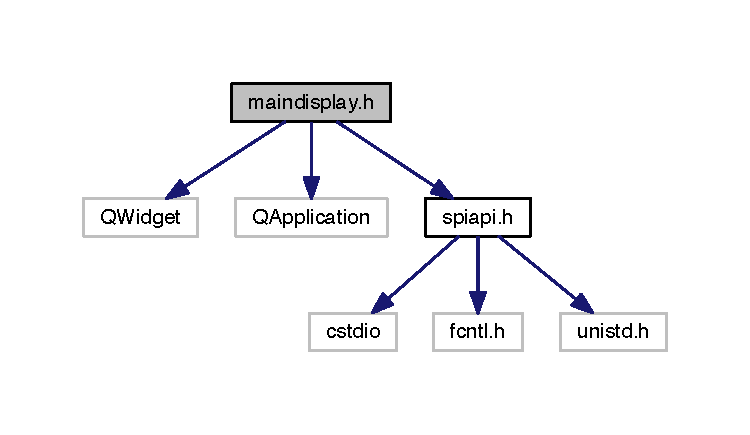
\includegraphics[width=350pt]{maindisplay_8h__incl}
\end{center}
\end{figure}
\subsubsection*{Datastrukturer}
\begin{DoxyCompactItemize}
\item 
class \hyperlink{class_main_display}{Main\+Display}
\end{DoxyCompactItemize}
\subsubsection*{Namespaces}
\begin{DoxyCompactItemize}
\item 
 \hyperlink{namespace_ui}{Ui}
\end{DoxyCompactItemize}


\subsubsection{Detaljeret beskrivelse}
Handles all U\+I-\/related in maindisplay including all tabs. 


\hypertarget{planner_8h}{}\subsection{planner.\+h filreference}
\label{planner_8h}\index{planner.\+h@{planner.\+h}}
{\ttfamily \#include $<$Q\+Widget$>$}\\*
Inklusions-\/afhængighedsgraf for planner.\+h\+:\nopagebreak
\begin{figure}[H]
\begin{center}
\leavevmode
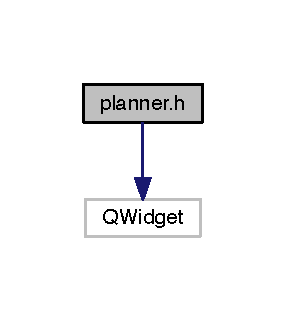
\includegraphics[width=137pt]{dc/def/planner_8h__incl}
\end{center}
\end{figure}
\subsubsection*{Datastrukturer}
\begin{DoxyCompactItemize}
\item 
class \hyperlink{class_planner}{Planner}
\end{DoxyCompactItemize}

\hypertarget{plannerdialog_8h}{}\subsection{plannerdialog.\+h filreference}
\label{plannerdialog_8h}\index{plannerdialog.\+h@{plannerdialog.\+h}}


Handles all U\+I-\/related in plannerdialog.  


{\ttfamily \#include $<$Q\+Dialog$>$}\\*
{\ttfamily \#include \char`\"{}plannerdialog.\+h\char`\"{}}\\*
Inklusions-\/afhængighedsgraf for plannerdialog.\+h\+:
\nopagebreak
\begin{figure}[H]
\begin{center}
\leavevmode
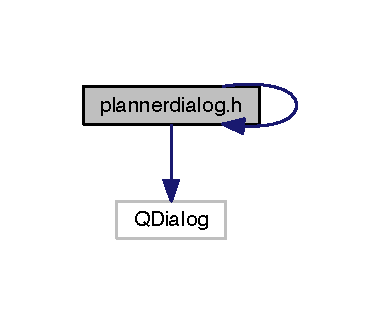
\includegraphics[width=182pt]{d5/d91/plannerdialog_8h__incl}
\end{center}
\end{figure}
Denne graf viser, hvilke filer der direkte eller indirekte inkluderer denne fil\+:
\nopagebreak
\begin{figure}[H]
\begin{center}
\leavevmode
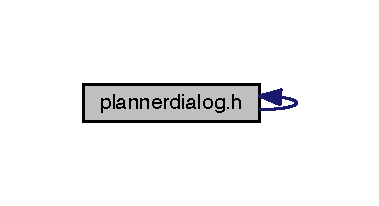
\includegraphics[width=182pt]{d9/df6/plannerdialog_8h__dep__incl}
\end{center}
\end{figure}
\subsubsection*{Datastrukturer}
\begin{DoxyCompactItemize}
\item 
class \hyperlink{class_planner_dialog}{Planner\+Dialog}
\end{DoxyCompactItemize}
\subsubsection*{Namespaces}
\begin{DoxyCompactItemize}
\item 
 \hyperlink{namespace_ui}{Ui}
\end{DoxyCompactItemize}


\subsubsection{Detaljeret beskrivelse}
Handles all U\+I-\/related in plannerdialog. 


\hypertarget{psoc__spi__cdrv_8c}{}\subsection{psoc\+\_\+spi\+\_\+cdrv.\+c filreference}
\label{psoc__spi__cdrv_8c}\index{psoc\+\_\+spi\+\_\+cdrv.\+c@{psoc\+\_\+spi\+\_\+cdrv.\+c}}
{\ttfamily \#include $<$linux/err.\+h$>$}\\*
{\ttfamily \#include $<$linux/ctype.\+h$>$}\\*
{\ttfamily \#include $<$linux/cdev.\+h$>$}\\*
{\ttfamily \#include $<$asm/uaccess.\+h$>$}\\*
{\ttfamily \#include $<$linux/input.\+h$>$}\\*
{\ttfamily \#include $<$linux/module.\+h$>$}\\*
{\ttfamily \#include \char`\"{}psoc\+\_\+spi\+\_\+dev.\+h\char`\"{}}\\*
Inklusions-\/afhængighedsgraf for psoc\+\_\+spi\+\_\+cdrv.\+c\+:
\nopagebreak
\begin{figure}[H]
\begin{center}
\leavevmode
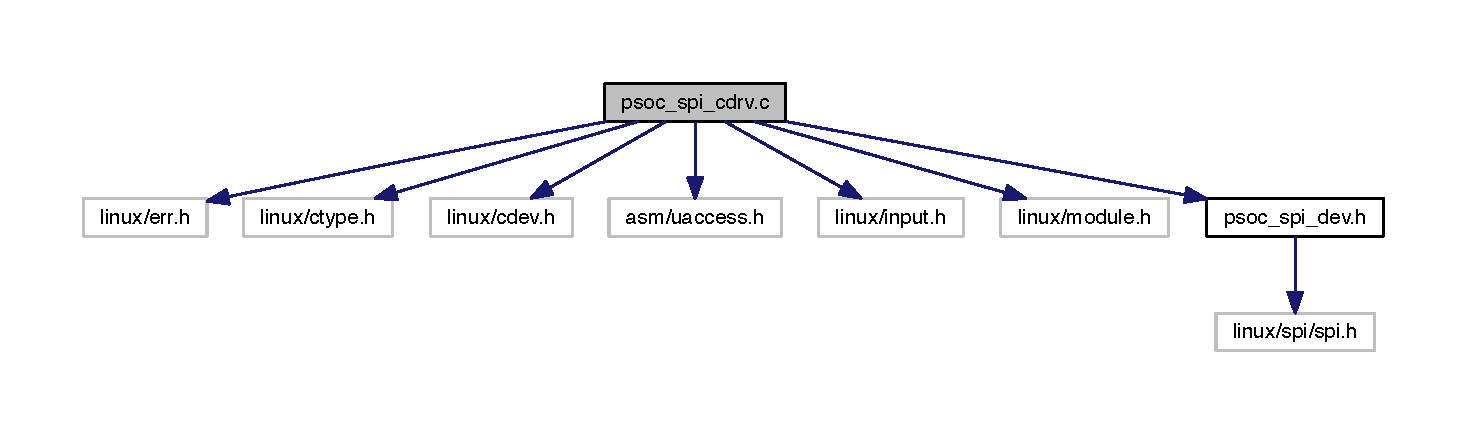
\includegraphics[width=350pt]{psoc__spi__cdrv_8c__incl}
\end{center}
\end{figure}
\subsubsection*{\#Defines}
\begin{DoxyCompactItemize}
\item 
\#define \hyperlink{psoc__spi__cdrv_8c_a124f980cd43bd8fc55e93146e383dfa1}{psoc4\+\_\+\+M\+A\+J\+OR}~64
\item 
\#define \hyperlink{psoc__spi__cdrv_8c_ad31e561878608dc6a09701bbc47fd6da}{psoc4\+\_\+\+M\+I\+N\+OR}~0
\item 
\#define \hyperlink{psoc__spi__cdrv_8c_a7a5b3d2485bcd2ccbb86c7e7cebe14e6}{psoc4\+\_\+\+D\+E\+V\+I\+CE}~1
\item 
\#define \hyperlink{psoc__spi__cdrv_8c_ae6648cd71a8bd49d58ae8ed33ba910d1}{M\+A\+X\+L\+EN}~16
\item 
\#define \hyperlink{psoc__spi__cdrv_8c_ae5874b45ddf4a96602ab046bb2bca80a}{M\+O\+D\+U\+L\+E\+\_\+\+D\+E\+B\+UG}~1
\item 
\#define \hyperlink{psoc__spi__cdrv_8c_aec31c17a958eb660efb41c39552beaff}{E\+R\+R\+G\+O\+TO}(label, ...)                                  
\end{DoxyCompactItemize}
\subsubsection*{Funktioner}
\begin{DoxyCompactItemize}
\item 
\hyperlink{psoc__spi__cdrv_8c_a76205f40e50e793bad85477c56a1fcb5}{M\+O\+D\+U\+L\+E\+\_\+\+A\+U\+T\+H\+OR} (\char`\"{}Jeppe Stærk\char`\"{})
\item 
\hyperlink{psoc__spi__cdrv_8c_a5c95e2cd11cba226f5f3513060a8928e}{M\+O\+D\+U\+L\+E\+\_\+\+L\+I\+C\+E\+N\+SE} (\char`\"{}Dual B\+SD/G\+PL\char`\"{})
\item 
static int \+\_\+\+\_\+init \hyperlink{psoc__spi__cdrv_8c_aab06beebbb38dd06b8e09548670afb21}{psoc4\+\_\+cdrv\+\_\+init} (void)
\item 
static void \+\_\+\+\_\+exit \hyperlink{psoc__spi__cdrv_8c_a016013e009a7cf15be35db2e3ec5d1f5}{psoc4\+\_\+cdrv\+\_\+exit} (void)
\item 
int \hyperlink{psoc__spi__cdrv_8c_a07168c0964966774fe208a05d9434cb1}{psoc4\+\_\+cdrv\+\_\+open} (struct inode $\ast$inode, struct file $\ast$filep)
\item 
int \hyperlink{psoc__spi__cdrv_8c_aa5f178db147ff43e6606e84bee03dc4e}{psoc4\+\_\+cdrv\+\_\+release} (struct inode $\ast$inode, struct file $\ast$filep)
\item 
ssize\+\_\+t \hyperlink{psoc__spi__cdrv_8c_a466ecffe904674771c9cff7f85590714}{psoc4\+\_\+cdrv\+\_\+write} (struct file $\ast$filep, const char \+\_\+\+\_\+user $\ast$ubuf, size\+\_\+t count, loff\+\_\+t $\ast$f\+\_\+pos)
\item 
ssize\+\_\+t \hyperlink{psoc__spi__cdrv_8c_a07b1fa48cf0fce6dafea41605b75d06c}{psoc4\+\_\+cdrv\+\_\+read} (struct file $\ast$filep, char \+\_\+\+\_\+user $\ast$ubuf, size\+\_\+t count, loff\+\_\+t $\ast$f\+\_\+pos)
\item 
\hyperlink{psoc__spi__cdrv_8c_a29681621922a8dc64ff84e750913f81a}{module\+\_\+init} (\hyperlink{psoc__spi__cdrv_8c_aab06beebbb38dd06b8e09548670afb21}{psoc4\+\_\+cdrv\+\_\+init})
\item 
\hyperlink{psoc__spi__cdrv_8c_a31b4f4d359c645ad1bb69792eff1f94b}{module\+\_\+exit} (\hyperlink{psoc__spi__cdrv_8c_a016013e009a7cf15be35db2e3ec5d1f5}{psoc4\+\_\+cdrv\+\_\+exit})
\end{DoxyCompactItemize}
\subsubsection*{Variable}
\begin{DoxyCompactItemize}
\item 
static struct cdev \hyperlink{psoc__spi__cdrv_8c_a333f62d9a833315715c266689805cf1a}{psoc4\+Dev}
\item 
struct file\+\_\+operations \hyperlink{psoc__spi__cdrv_8c_a867a6cfbce3482b70eb142dd2067774f}{psoc4\+\_\+\+Fops}
\item 
static int \hyperlink{psoc__spi__cdrv_8c_a68915ca671494de990d424ea3a02d7e9}{devno}
\item 
static struct spi\+\_\+device $\ast$ \hyperlink{psoc__spi__cdrv_8c_a777bc87492fc7e5d359aa1f0450fc370}{psoc4\+\_\+spi\+\_\+device} = N\+U\+LL
\end{DoxyCompactItemize}


\subsubsection{\#Define-\/dokumentation}
\index{psoc\+\_\+spi\+\_\+cdrv.\+c@{psoc\+\_\+spi\+\_\+cdrv.\+c}!E\+R\+R\+G\+O\+TO@{E\+R\+R\+G\+O\+TO}}
\index{E\+R\+R\+G\+O\+TO@{E\+R\+R\+G\+O\+TO}!psoc\+\_\+spi\+\_\+cdrv.\+c@{psoc\+\_\+spi\+\_\+cdrv.\+c}}
\paragraph[{\texorpdfstring{E\+R\+R\+G\+O\+TO}{ERRGOTO}}]{\setlength{\rightskip}{0pt plus 5cm}\#define E\+R\+R\+G\+O\+TO(
\begin{DoxyParamCaption}
\item[{}]{label, }
\item[{}]{...}
\end{DoxyParamCaption}
)}\hypertarget{psoc__spi__cdrv_8c_aec31c17a958eb660efb41c39552beaff}{}\label{psoc__spi__cdrv_8c_aec31c17a958eb660efb41c39552beaff}
{\bfseries Værdi\+:}
\begin{DoxyCode}
\{                                             \(\backslash\)
    printk (\_\_VA\_ARGS\_\_);                     \(\backslash\)
    goto label;                               \(\backslash\)
\} \textcolor{keywordflow}{while}(0)
\end{DoxyCode}


Defineret på linje 28 i filen psoc\+\_\+spi\+\_\+cdrv.\+c.



Refereret til af psoc4\+\_\+cdrv\+\_\+init().

\index{psoc\+\_\+spi\+\_\+cdrv.\+c@{psoc\+\_\+spi\+\_\+cdrv.\+c}!M\+A\+X\+L\+EN@{M\+A\+X\+L\+EN}}
\index{M\+A\+X\+L\+EN@{M\+A\+X\+L\+EN}!psoc\+\_\+spi\+\_\+cdrv.\+c@{psoc\+\_\+spi\+\_\+cdrv.\+c}}
\paragraph[{\texorpdfstring{M\+A\+X\+L\+EN}{MAXLEN}}]{\setlength{\rightskip}{0pt plus 5cm}\#define M\+A\+X\+L\+EN~16}\hypertarget{psoc__spi__cdrv_8c_ae6648cd71a8bd49d58ae8ed33ba910d1}{}\label{psoc__spi__cdrv_8c_ae6648cd71a8bd49d58ae8ed33ba910d1}


Defineret på linje 15 i filen psoc\+\_\+spi\+\_\+cdrv.\+c.



Refereret til af psoc4\+\_\+cdrv\+\_\+write().

\index{psoc\+\_\+spi\+\_\+cdrv.\+c@{psoc\+\_\+spi\+\_\+cdrv.\+c}!M\+O\+D\+U\+L\+E\+\_\+\+D\+E\+B\+UG@{M\+O\+D\+U\+L\+E\+\_\+\+D\+E\+B\+UG}}
\index{M\+O\+D\+U\+L\+E\+\_\+\+D\+E\+B\+UG@{M\+O\+D\+U\+L\+E\+\_\+\+D\+E\+B\+UG}!psoc\+\_\+spi\+\_\+cdrv.\+c@{psoc\+\_\+spi\+\_\+cdrv.\+c}}
\paragraph[{\texorpdfstring{M\+O\+D\+U\+L\+E\+\_\+\+D\+E\+B\+UG}{MODULE_DEBUG}}]{\setlength{\rightskip}{0pt plus 5cm}\#define M\+O\+D\+U\+L\+E\+\_\+\+D\+E\+B\+UG~1}\hypertarget{psoc__spi__cdrv_8c_ae5874b45ddf4a96602ab046bb2bca80a}{}\label{psoc__spi__cdrv_8c_ae5874b45ddf4a96602ab046bb2bca80a}


Defineret på linje 17 i filen psoc\+\_\+spi\+\_\+cdrv.\+c.



Refereret til af psoc4\+\_\+cdrv\+\_\+read() og psoc4\+\_\+cdrv\+\_\+write().

\index{psoc\+\_\+spi\+\_\+cdrv.\+c@{psoc\+\_\+spi\+\_\+cdrv.\+c}!psoc4\+\_\+\+D\+E\+V\+I\+CE@{psoc4\+\_\+\+D\+E\+V\+I\+CE}}
\index{psoc4\+\_\+\+D\+E\+V\+I\+CE@{psoc4\+\_\+\+D\+E\+V\+I\+CE}!psoc\+\_\+spi\+\_\+cdrv.\+c@{psoc\+\_\+spi\+\_\+cdrv.\+c}}
\paragraph[{\texorpdfstring{psoc4\+\_\+\+D\+E\+V\+I\+CE}{psoc4_DEVICE}}]{\setlength{\rightskip}{0pt plus 5cm}\#define psoc4\+\_\+\+D\+E\+V\+I\+CE~1}\hypertarget{psoc__spi__cdrv_8c_a7a5b3d2485bcd2ccbb86c7e7cebe14e6}{}\label{psoc__spi__cdrv_8c_a7a5b3d2485bcd2ccbb86c7e7cebe14e6}


Defineret på linje 14 i filen psoc\+\_\+spi\+\_\+cdrv.\+c.



Refereret til af psoc4\+\_\+cdrv\+\_\+exit(), psoc4\+\_\+cdrv\+\_\+init(), psoc4\+\_\+cdrv\+\_\+open() og psoc4\+\_\+cdrv\+\_\+release().

\index{psoc\+\_\+spi\+\_\+cdrv.\+c@{psoc\+\_\+spi\+\_\+cdrv.\+c}!psoc4\+\_\+\+M\+A\+J\+OR@{psoc4\+\_\+\+M\+A\+J\+OR}}
\index{psoc4\+\_\+\+M\+A\+J\+OR@{psoc4\+\_\+\+M\+A\+J\+OR}!psoc\+\_\+spi\+\_\+cdrv.\+c@{psoc\+\_\+spi\+\_\+cdrv.\+c}}
\paragraph[{\texorpdfstring{psoc4\+\_\+\+M\+A\+J\+OR}{psoc4_MAJOR}}]{\setlength{\rightskip}{0pt plus 5cm}\#define psoc4\+\_\+\+M\+A\+J\+OR~64}\hypertarget{psoc__spi__cdrv_8c_a124f980cd43bd8fc55e93146e383dfa1}{}\label{psoc__spi__cdrv_8c_a124f980cd43bd8fc55e93146e383dfa1}


Defineret på linje 12 i filen psoc\+\_\+spi\+\_\+cdrv.\+c.



Refereret til af psoc4\+\_\+cdrv\+\_\+init().

\index{psoc\+\_\+spi\+\_\+cdrv.\+c@{psoc\+\_\+spi\+\_\+cdrv.\+c}!psoc4\+\_\+\+M\+I\+N\+OR@{psoc4\+\_\+\+M\+I\+N\+OR}}
\index{psoc4\+\_\+\+M\+I\+N\+OR@{psoc4\+\_\+\+M\+I\+N\+OR}!psoc\+\_\+spi\+\_\+cdrv.\+c@{psoc\+\_\+spi\+\_\+cdrv.\+c}}
\paragraph[{\texorpdfstring{psoc4\+\_\+\+M\+I\+N\+OR}{psoc4_MINOR}}]{\setlength{\rightskip}{0pt plus 5cm}\#define psoc4\+\_\+\+M\+I\+N\+OR~0}\hypertarget{psoc__spi__cdrv_8c_ad31e561878608dc6a09701bbc47fd6da}{}\label{psoc__spi__cdrv_8c_ad31e561878608dc6a09701bbc47fd6da}


Defineret på linje 13 i filen psoc\+\_\+spi\+\_\+cdrv.\+c.



Refereret til af psoc4\+\_\+cdrv\+\_\+init().



\subsubsection{Funktions-\/dokumentation}
\index{psoc\+\_\+spi\+\_\+cdrv.\+c@{psoc\+\_\+spi\+\_\+cdrv.\+c}!M\+O\+D\+U\+L\+E\+\_\+\+A\+U\+T\+H\+OR@{M\+O\+D\+U\+L\+E\+\_\+\+A\+U\+T\+H\+OR}}
\index{M\+O\+D\+U\+L\+E\+\_\+\+A\+U\+T\+H\+OR@{M\+O\+D\+U\+L\+E\+\_\+\+A\+U\+T\+H\+OR}!psoc\+\_\+spi\+\_\+cdrv.\+c@{psoc\+\_\+spi\+\_\+cdrv.\+c}}
\paragraph[{\texorpdfstring{M\+O\+D\+U\+L\+E\+\_\+\+A\+U\+T\+H\+O\+R(""Jeppe Stærk"")}{MODULE_AUTHOR("Jeppe Stærk")}}]{\setlength{\rightskip}{0pt plus 5cm}M\+O\+D\+U\+L\+E\+\_\+\+A\+U\+T\+H\+OR (
\begin{DoxyParamCaption}
\item[{\char`\"{}Jeppe Stærk\char`\"{}}]{}
\end{DoxyParamCaption}
)}\hypertarget{psoc__spi__cdrv_8c_a76205f40e50e793bad85477c56a1fcb5}{}\label{psoc__spi__cdrv_8c_a76205f40e50e793bad85477c56a1fcb5}
\index{psoc\+\_\+spi\+\_\+cdrv.\+c@{psoc\+\_\+spi\+\_\+cdrv.\+c}!module\+\_\+exit@{module\+\_\+exit}}
\index{module\+\_\+exit@{module\+\_\+exit}!psoc\+\_\+spi\+\_\+cdrv.\+c@{psoc\+\_\+spi\+\_\+cdrv.\+c}}
\paragraph[{\texorpdfstring{module\+\_\+exit(psoc4\+\_\+cdrv\+\_\+exit)}{module_exit(psoc4_cdrv_exit)}}]{\setlength{\rightskip}{0pt plus 5cm}module\+\_\+exit (
\begin{DoxyParamCaption}
\item[{{\bf psoc4\+\_\+cdrv\+\_\+exit}}]{}
\end{DoxyParamCaption}
)}\hypertarget{psoc__spi__cdrv_8c_a31b4f4d359c645ad1bb69792eff1f94b}{}\label{psoc__spi__cdrv_8c_a31b4f4d359c645ad1bb69792eff1f94b}


Refereret til af psoc4\+\_\+cdrv\+\_\+read().



Her er kalder-\/grafen for denne funktion\+:
\nopagebreak
\begin{figure}[H]
\begin{center}
\leavevmode
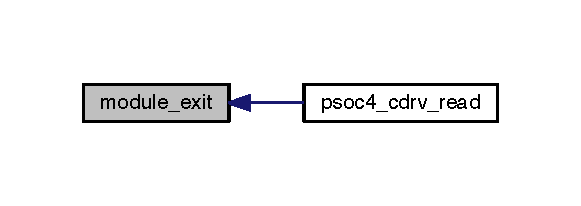
\includegraphics[width=279pt]{psoc__spi__cdrv_8c_a31b4f4d359c645ad1bb69792eff1f94b_icgraph}
\end{center}
\end{figure}


\index{psoc\+\_\+spi\+\_\+cdrv.\+c@{psoc\+\_\+spi\+\_\+cdrv.\+c}!module\+\_\+init@{module\+\_\+init}}
\index{module\+\_\+init@{module\+\_\+init}!psoc\+\_\+spi\+\_\+cdrv.\+c@{psoc\+\_\+spi\+\_\+cdrv.\+c}}
\paragraph[{\texorpdfstring{module\+\_\+init(psoc4\+\_\+cdrv\+\_\+init)}{module_init(psoc4_cdrv_init)}}]{\setlength{\rightskip}{0pt plus 5cm}module\+\_\+init (
\begin{DoxyParamCaption}
\item[{{\bf psoc4\+\_\+cdrv\+\_\+init}}]{}
\end{DoxyParamCaption}
)}\hypertarget{psoc__spi__cdrv_8c_a29681621922a8dc64ff84e750913f81a}{}\label{psoc__spi__cdrv_8c_a29681621922a8dc64ff84e750913f81a}


Refereret til af psoc4\+\_\+cdrv\+\_\+read().



Her er kalder-\/grafen for denne funktion\+:
\nopagebreak
\begin{figure}[H]
\begin{center}
\leavevmode
\includegraphics[width=276pt]{psoc__spi__cdrv_8c_a29681621922a8dc64ff84e750913f81a_icgraph}
\end{center}
\end{figure}


\index{psoc\+\_\+spi\+\_\+cdrv.\+c@{psoc\+\_\+spi\+\_\+cdrv.\+c}!M\+O\+D\+U\+L\+E\+\_\+\+L\+I\+C\+E\+N\+SE@{M\+O\+D\+U\+L\+E\+\_\+\+L\+I\+C\+E\+N\+SE}}
\index{M\+O\+D\+U\+L\+E\+\_\+\+L\+I\+C\+E\+N\+SE@{M\+O\+D\+U\+L\+E\+\_\+\+L\+I\+C\+E\+N\+SE}!psoc\+\_\+spi\+\_\+cdrv.\+c@{psoc\+\_\+spi\+\_\+cdrv.\+c}}
\paragraph[{\texorpdfstring{M\+O\+D\+U\+L\+E\+\_\+\+L\+I\+C\+E\+N\+S\+E(""Dual B\+S\+D/\+G\+PL"")}{MODULE_LICENSE("Dual BSD/GPL")}}]{\setlength{\rightskip}{0pt plus 5cm}M\+O\+D\+U\+L\+E\+\_\+\+L\+I\+C\+E\+N\+SE (
\begin{DoxyParamCaption}
\item[{\char`\"{}Dual B\+SD/G\+PL\char`\"{}}]{}
\end{DoxyParamCaption}
)}\hypertarget{psoc__spi__cdrv_8c_a5c95e2cd11cba226f5f3513060a8928e}{}\label{psoc__spi__cdrv_8c_a5c95e2cd11cba226f5f3513060a8928e}
\index{psoc\+\_\+spi\+\_\+cdrv.\+c@{psoc\+\_\+spi\+\_\+cdrv.\+c}!psoc4\+\_\+cdrv\+\_\+exit@{psoc4\+\_\+cdrv\+\_\+exit}}
\index{psoc4\+\_\+cdrv\+\_\+exit@{psoc4\+\_\+cdrv\+\_\+exit}!psoc\+\_\+spi\+\_\+cdrv.\+c@{psoc\+\_\+spi\+\_\+cdrv.\+c}}
\paragraph[{\texorpdfstring{psoc4\+\_\+cdrv\+\_\+exit(void)}{psoc4_cdrv_exit(void)}}]{\setlength{\rightskip}{0pt plus 5cm}static void \+\_\+\+\_\+exit psoc4\+\_\+cdrv\+\_\+exit (
\begin{DoxyParamCaption}
\item[{void}]{}
\end{DoxyParamCaption}
)\hspace{0.3cm}{\ttfamily [static]}}\hypertarget{psoc__spi__cdrv_8c_a016013e009a7cf15be35db2e3ec5d1f5}{}\label{psoc__spi__cdrv_8c_a016013e009a7cf15be35db2e3ec5d1f5}


Defineret på linje 74 i filen psoc\+\_\+spi\+\_\+cdrv.\+c.



Indeholder referencer til devno, psoc4\+\_\+\+D\+E\+V\+I\+CE, psoc4\+\_\+spi\+\_\+exit() og psoc4\+Dev.



Refereret til af psoc4\+\_\+cdrv\+\_\+read().


\begin{DoxyCode}
75 \{
76     printk(\textcolor{stringliteral}{"psoc4 driver Exit\(\backslash\)n"});
77     cdev\_del(&\hyperlink{psoc__spi__cdrv_8c_a333f62d9a833315715c266689805cf1a}{psoc4Dev});
78     
79     unregister\_chrdev\_region(\hyperlink{psoc__spi__cdrv_8c_a68915ca671494de990d424ea3a02d7e9}{devno}, \hyperlink{psoc__spi__cdrv_8c_a7a5b3d2485bcd2ccbb86c7e7cebe14e6}{psoc4\_DEVICE});
80     
81     \hyperlink{psoc__spi__dev_8c_a9d271797d6983fd0f289b7f6b266d0be}{psoc4\_spi\_exit}();
82 \}
\end{DoxyCode}


Her er kald-\/grafen for denne funktion\+:
\nopagebreak
\begin{figure}[H]
\begin{center}
\leavevmode
\includegraphics[width=286pt]{psoc__spi__cdrv_8c_a016013e009a7cf15be35db2e3ec5d1f5_cgraph}
\end{center}
\end{figure}




Her er kalder-\/grafen for denne funktion\+:
\nopagebreak
\begin{figure}[H]
\begin{center}
\leavevmode
\includegraphics[width=297pt]{psoc__spi__cdrv_8c_a016013e009a7cf15be35db2e3ec5d1f5_icgraph}
\end{center}
\end{figure}


\index{psoc\+\_\+spi\+\_\+cdrv.\+c@{psoc\+\_\+spi\+\_\+cdrv.\+c}!psoc4\+\_\+cdrv\+\_\+init@{psoc4\+\_\+cdrv\+\_\+init}}
\index{psoc4\+\_\+cdrv\+\_\+init@{psoc4\+\_\+cdrv\+\_\+init}!psoc\+\_\+spi\+\_\+cdrv.\+c@{psoc\+\_\+spi\+\_\+cdrv.\+c}}
\paragraph[{\texorpdfstring{psoc4\+\_\+cdrv\+\_\+init(void)}{psoc4_cdrv_init(void)}}]{\setlength{\rightskip}{0pt plus 5cm}static int \+\_\+\+\_\+init psoc4\+\_\+cdrv\+\_\+init (
\begin{DoxyParamCaption}
\item[{void}]{}
\end{DoxyParamCaption}
)\hspace{0.3cm}{\ttfamily [static]}}\hypertarget{psoc__spi__cdrv_8c_aab06beebbb38dd06b8e09548670afb21}{}\label{psoc__spi__cdrv_8c_aab06beebbb38dd06b8e09548670afb21}


Defineret på linje 38 i filen psoc\+\_\+spi\+\_\+cdrv.\+c.



Indeholder referencer til devno, E\+R\+R\+G\+O\+TO, psoc4\+\_\+\+D\+E\+V\+I\+CE, psoc4\+\_\+\+Fops, psoc4\+\_\+\+M\+A\+J\+OR, psoc4\+\_\+\+M\+I\+N\+OR, psoc4\+\_\+spi\+\_\+exit(), psoc4\+\_\+spi\+\_\+init() og psoc4\+Dev.



Refereret til af psoc4\+\_\+cdrv\+\_\+read().


\begin{DoxyCode}
39 \{
40     \textcolor{keywordtype}{int} err;
41     
42     printk(\textcolor{stringliteral}{"psoc4 driver initializing\(\backslash\)n"});
43     
44     \textcolor{comment}{/* Register SPI Driver */}
45     err=\hyperlink{psoc__spi__dev_8c_a8d33dfea48e2a1e88f7758492ede12cf}{psoc4\_spi\_init}();
46     \textcolor{keywordflow}{if}(err)
47         \hyperlink{psoc__spi__cdrv_8c_aec31c17a958eb660efb41c39552beaff}{ERRGOTO}(error, \textcolor{stringliteral}{"Failed SPI Initialization\(\backslash\)n"});
48     
49     \textcolor{comment}{/* Allocate chrdev region */}
50     \hyperlink{psoc__spi__cdrv_8c_a68915ca671494de990d424ea3a02d7e9}{devno} = MKDEV(\hyperlink{psoc__spi__cdrv_8c_a124f980cd43bd8fc55e93146e383dfa1}{psoc4\_MAJOR}, \hyperlink{psoc__spi__cdrv_8c_ad31e561878608dc6a09701bbc47fd6da}{psoc4\_MINOR});
51     err = register\_chrdev\_region(\hyperlink{psoc__spi__cdrv_8c_a68915ca671494de990d424ea3a02d7e9}{devno}, \hyperlink{psoc__spi__cdrv_8c_a7a5b3d2485bcd2ccbb86c7e7cebe14e6}{psoc4\_DEVICE}, \textcolor{stringliteral}{"psoc4"});
52     \textcolor{keywordflow}{if}(err)
53         \hyperlink{psoc__spi__cdrv_8c_aec31c17a958eb660efb41c39552beaff}{ERRGOTO}(err\_spi\_init, \textcolor{stringliteral}{"Failed registering char region (%d,%d) +%d, error %d\(\backslash\)n"},
54                 \hyperlink{psoc__spi__cdrv_8c_a124f980cd43bd8fc55e93146e383dfa1}{psoc4\_MAJOR}, \hyperlink{psoc__spi__cdrv_8c_ad31e561878608dc6a09701bbc47fd6da}{psoc4\_MINOR}, \hyperlink{psoc__spi__cdrv_8c_a7a5b3d2485bcd2ccbb86c7e7cebe14e6}{psoc4\_DEVICE}, err);
55     
56     \textcolor{comment}{/* Register Char Device */}
57     cdev\_init(&\hyperlink{psoc__spi__cdrv_8c_a333f62d9a833315715c266689805cf1a}{psoc4Dev}, &\hyperlink{psoc__spi__cdrv_8c_a867a6cfbce3482b70eb142dd2067774f}{psoc4\_Fops});
58     err = cdev\_add(&\hyperlink{psoc__spi__cdrv_8c_a333f62d9a833315715c266689805cf1a}{psoc4Dev}, \hyperlink{psoc__spi__cdrv_8c_a68915ca671494de990d424ea3a02d7e9}{devno}, \hyperlink{psoc__spi__cdrv_8c_a7a5b3d2485bcd2ccbb86c7e7cebe14e6}{psoc4\_DEVICE});
59     \textcolor{keywordflow}{if} (err)
60         \hyperlink{psoc__spi__cdrv_8c_aec31c17a958eb660efb41c39552beaff}{ERRGOTO}(err\_register, \textcolor{stringliteral}{"Error %d adding psoc4 device\(\backslash\)n"}, err);
61     
62     \textcolor{keywordflow}{return} 0;
63     
64 err\_register:
65     unregister\_chrdev\_region(\hyperlink{psoc__spi__cdrv_8c_a68915ca671494de990d424ea3a02d7e9}{devno}, \hyperlink{psoc__spi__cdrv_8c_a7a5b3d2485bcd2ccbb86c7e7cebe14e6}{psoc4\_DEVICE});
66     
67 err\_spi\_init:
68     \hyperlink{psoc__spi__dev_8c_a9d271797d6983fd0f289b7f6b266d0be}{psoc4\_spi\_exit}();
69     
70 error:
71     \textcolor{keywordflow}{return} err;
72 \}
\end{DoxyCode}


Her er kald-\/grafen for denne funktion\+:
\nopagebreak
\begin{figure}[H]
\begin{center}
\leavevmode
\includegraphics[width=284pt]{psoc__spi__cdrv_8c_aab06beebbb38dd06b8e09548670afb21_cgraph}
\end{center}
\end{figure}




Her er kalder-\/grafen for denne funktion\+:
\nopagebreak
\begin{figure}[H]
\begin{center}
\leavevmode
\includegraphics[width=294pt]{psoc__spi__cdrv_8c_aab06beebbb38dd06b8e09548670afb21_icgraph}
\end{center}
\end{figure}


\index{psoc\+\_\+spi\+\_\+cdrv.\+c@{psoc\+\_\+spi\+\_\+cdrv.\+c}!psoc4\+\_\+cdrv\+\_\+open@{psoc4\+\_\+cdrv\+\_\+open}}
\index{psoc4\+\_\+cdrv\+\_\+open@{psoc4\+\_\+cdrv\+\_\+open}!psoc\+\_\+spi\+\_\+cdrv.\+c@{psoc\+\_\+spi\+\_\+cdrv.\+c}}
\paragraph[{\texorpdfstring{psoc4\+\_\+cdrv\+\_\+open(struct inode $\ast$inode, struct file $\ast$filep)}{psoc4_cdrv_open(struct inode *inode, struct file *filep)}}]{\setlength{\rightskip}{0pt plus 5cm}int psoc4\+\_\+cdrv\+\_\+open (
\begin{DoxyParamCaption}
\item[{struct inode $\ast$}]{inode, }
\item[{struct file $\ast$}]{filep}
\end{DoxyParamCaption}
)}\hypertarget{psoc__spi__cdrv_8c_a07168c0964966774fe208a05d9434cb1}{}\label{psoc__spi__cdrv_8c_a07168c0964966774fe208a05d9434cb1}


Defineret på linje 84 i filen psoc\+\_\+spi\+\_\+cdrv.\+c.



Indeholder referencer til psoc4\+\_\+\+D\+E\+V\+I\+CE, psoc4\+\_\+get\+\_\+device() og psoc4\+\_\+spi\+\_\+device.



Refereret til af psoc4\+\_\+cdrv\+\_\+read().


\begin{DoxyCode}
85 \{
86     \textcolor{keywordtype}{int} major = imajor(inode);
87     \textcolor{keywordtype}{int} minor = iminor(inode);
88     
89     printk(\textcolor{stringliteral}{"cdrv\_open: Opening psoc4 Device [major], [minor]: %i, %i\(\backslash\)n"}, major, minor);
90     
91     \textcolor{comment}{/* Check if minor number is within range */}
92     \textcolor{keywordflow}{if} (minor > \hyperlink{psoc__spi__cdrv_8c_a7a5b3d2485bcd2ccbb86c7e7cebe14e6}{psoc4\_DEVICE}-1)
93     \{
94         printk(\textcolor{stringliteral}{"Minor no out of range (0-%i): %i\(\backslash\)n"}, \hyperlink{psoc__spi__cdrv_8c_a7a5b3d2485bcd2ccbb86c7e7cebe14e6}{psoc4\_DEVICE}, minor);
95         \textcolor{keywordflow}{return} -ENODEV;
96     \}
97     
98     \textcolor{comment}{/* Check if a psoc4 device is registered */}
99     \textcolor{keywordflow}{if}(!(\hyperlink{psoc__spi__cdrv_8c_a777bc87492fc7e5d359aa1f0450fc370}{psoc4\_spi\_device}=\hyperlink{psoc__spi__dev_8c_a2870b5e4e3611c8ba3baf9592c4d8be1}{psoc4\_get\_device}()))
100         \textcolor{keywordflow}{return} -ENODEV;
101     
102     \textcolor{keywordflow}{return} 0;
103 \}
\end{DoxyCode}


Her er kald-\/grafen for denne funktion\+:
\nopagebreak
\begin{figure}[H]
\begin{center}
\leavevmode
\includegraphics[width=308pt]{psoc__spi__cdrv_8c_a07168c0964966774fe208a05d9434cb1_cgraph}
\end{center}
\end{figure}




Her er kalder-\/grafen for denne funktion\+:
\nopagebreak
\begin{figure}[H]
\begin{center}
\leavevmode
\includegraphics[width=304pt]{psoc__spi__cdrv_8c_a07168c0964966774fe208a05d9434cb1_icgraph}
\end{center}
\end{figure}


\index{psoc\+\_\+spi\+\_\+cdrv.\+c@{psoc\+\_\+spi\+\_\+cdrv.\+c}!psoc4\+\_\+cdrv\+\_\+read@{psoc4\+\_\+cdrv\+\_\+read}}
\index{psoc4\+\_\+cdrv\+\_\+read@{psoc4\+\_\+cdrv\+\_\+read}!psoc\+\_\+spi\+\_\+cdrv.\+c@{psoc\+\_\+spi\+\_\+cdrv.\+c}}
\paragraph[{\texorpdfstring{psoc4\+\_\+cdrv\+\_\+read(struct file $\ast$filep, char \+\_\+\+\_\+user $\ast$ubuf, size\+\_\+t count, loff\+\_\+t $\ast$f\+\_\+pos)}{psoc4_cdrv_read(struct file *filep, char __user *ubuf, size_t count, loff_t *f_pos)}}]{\setlength{\rightskip}{0pt plus 5cm}ssize\+\_\+t psoc4\+\_\+cdrv\+\_\+read (
\begin{DoxyParamCaption}
\item[{struct file $\ast$}]{filep, }
\item[{char \+\_\+\+\_\+user $\ast$}]{ubuf, }
\item[{size\+\_\+t}]{count, }
\item[{loff\+\_\+t $\ast$}]{f\+\_\+pos}
\end{DoxyParamCaption}
)}\hypertarget{psoc__spi__cdrv_8c_a07b1fa48cf0fce6dafea41605b75d06c}{}\label{psoc__spi__cdrv_8c_a07b1fa48cf0fce6dafea41605b75d06c}


Defineret på linje 158 i filen psoc\+\_\+spi\+\_\+cdrv.\+c.



Indeholder referencer til M\+O\+D\+U\+L\+E\+\_\+\+D\+E\+B\+UG, module\+\_\+exit(), module\+\_\+init(), psoc4\+\_\+cdrv\+\_\+exit(), psoc4\+\_\+cdrv\+\_\+init(), psoc4\+\_\+cdrv\+\_\+open(), psoc4\+\_\+cdrv\+\_\+release(), psoc4\+\_\+cdrv\+\_\+write(), psoc4\+\_\+\+Fops, psoc4\+\_\+spi\+\_\+device og psoc4\+\_\+spi\+\_\+read().


\begin{DoxyCode}
159 \{
160     \textcolor{keywordtype}{int} minor, rxLen;
161     u16 rxData;
162     \textcolor{keywordtype}{char} rxBuffer[5];
163     
164     minor = iminor(filep->f\_inode);
165     
166     \textcolor{keywordflow}{if}(\hyperlink{psoc__spi__cdrv_8c_ae5874b45ddf4a96602ab046bb2bca80a}{MODULE\_DEBUG})
167         printk(KERN\_ALERT \textcolor{stringliteral}{"cdrv\_read: Reading from psoc4 [Minor] %i \(\backslash\)n"}, minor);
168     
169     \hyperlink{psoc__spi__dev_8c_aafd69a02e9977933fb6789e99d296bee}{psoc4\_spi\_read}(\hyperlink{psoc__spi__cdrv_8c_a777bc87492fc7e5d359aa1f0450fc370}{psoc4\_spi\_device}, &rxData);
170     
171     \textcolor{keywordflow}{if}(\hyperlink{psoc__spi__cdrv_8c_ae5874b45ddf4a96602ab046bb2bca80a}{MODULE\_DEBUG})
172         printk(KERN\_DEBUG \textcolor{stringliteral}{"cdrv\_read: Reading from psoc4 result: 0x%02x\(\backslash\)n"}, rxData);
173         
174     \textcolor{comment}{// Laver en int om til en string}
175     \textcolor{comment}{/* Convert to string and copy to user space */}
176     \textcolor{comment}{//  len = snprintf(resultBuf, sizeof resultBuf, "%d\(\backslash\)n", result);}
177     \textcolor{comment}{/* Convert integer to string limited to "count" size. Returns}
178 \textcolor{comment}{    * length excluding NULL termination */}
179     rxLen = sprintf(rxBuffer, \textcolor{stringliteral}{"%hu"}, rxData);
180     rxLen++;
181 
182     \textcolor{keywordflow}{if}(\hyperlink{psoc__spi__cdrv_8c_ae5874b45ddf4a96602ab046bb2bca80a}{MODULE\_DEBUG})
183         printk(KERN\_DEBUG \textcolor{stringliteral}{"cdrv\_read: Convert from psoc4 result: %s \(\backslash\)n"}, rxBuffer);
184 
185     \textcolor{comment}{/* Copy data to user space */}
186     \textcolor{keywordflow}{if}(copy\_to\_user(ubuf, rxBuffer, rxLen))
187         \textcolor{keywordflow}{return} -EFAULT;
188 
189     \textcolor{comment}{/* Move fileptr */}
190     *f\_pos += rxLen;
191     
192     \textcolor{keywordflow}{return} rxLen;
193 \}
\end{DoxyCode}


Her er kald-\/grafen for denne funktion\+:
\nopagebreak
\begin{figure}[H]
\begin{center}
\leavevmode
\includegraphics[width=350pt]{psoc__spi__cdrv_8c_a07b1fa48cf0fce6dafea41605b75d06c_cgraph}
\end{center}
\end{figure}


\index{psoc\+\_\+spi\+\_\+cdrv.\+c@{psoc\+\_\+spi\+\_\+cdrv.\+c}!psoc4\+\_\+cdrv\+\_\+release@{psoc4\+\_\+cdrv\+\_\+release}}
\index{psoc4\+\_\+cdrv\+\_\+release@{psoc4\+\_\+cdrv\+\_\+release}!psoc\+\_\+spi\+\_\+cdrv.\+c@{psoc\+\_\+spi\+\_\+cdrv.\+c}}
\paragraph[{\texorpdfstring{psoc4\+\_\+cdrv\+\_\+release(struct inode $\ast$inode, struct file $\ast$filep)}{psoc4_cdrv_release(struct inode *inode, struct file *filep)}}]{\setlength{\rightskip}{0pt plus 5cm}int psoc4\+\_\+cdrv\+\_\+release (
\begin{DoxyParamCaption}
\item[{struct inode $\ast$}]{inode, }
\item[{struct file $\ast$}]{filep}
\end{DoxyParamCaption}
)}\hypertarget{psoc__spi__cdrv_8c_aa5f178db147ff43e6606e84bee03dc4e}{}\label{psoc__spi__cdrv_8c_aa5f178db147ff43e6606e84bee03dc4e}


Defineret på linje 105 i filen psoc\+\_\+spi\+\_\+cdrv.\+c.



Indeholder referencer til psoc4\+\_\+\+D\+E\+V\+I\+CE, psoc4\+\_\+get\+\_\+device() og psoc4\+\_\+spi\+\_\+device.



Refereret til af psoc4\+\_\+cdrv\+\_\+read().


\begin{DoxyCode}
106 \{
107     \textcolor{keywordtype}{int} major = imajor(inode);
108     \textcolor{keywordtype}{int} minor = iminor(inode);
109     
110     printk(\textcolor{stringliteral}{"cdrv\_release: Closing psoc4 Device [major], [minor]: %i, %i\(\backslash\)n"}, major, minor);
111     
112     \textcolor{keywordflow}{if} ((minor > \hyperlink{psoc__spi__cdrv_8c_a7a5b3d2485bcd2ccbb86c7e7cebe14e6}{psoc4\_DEVICE}-1) || !(\hyperlink{psoc__spi__cdrv_8c_a777bc87492fc7e5d359aa1f0450fc370}{psoc4\_spi\_device}=
      \hyperlink{psoc__spi__dev_8c_a2870b5e4e3611c8ba3baf9592c4d8be1}{psoc4\_get\_device}()))
113         \textcolor{keywordflow}{return} -ENODEV;
114     
115     \textcolor{keywordflow}{return} 0;
116 \}
\end{DoxyCode}


Her er kald-\/grafen for denne funktion\+:
\nopagebreak
\begin{figure}[H]
\begin{center}
\leavevmode
\includegraphics[width=318pt]{psoc__spi__cdrv_8c_aa5f178db147ff43e6606e84bee03dc4e_cgraph}
\end{center}
\end{figure}




Her er kalder-\/grafen for denne funktion\+:
\nopagebreak
\begin{figure}[H]
\begin{center}
\leavevmode
\includegraphics[width=314pt]{psoc__spi__cdrv_8c_aa5f178db147ff43e6606e84bee03dc4e_icgraph}
\end{center}
\end{figure}


\index{psoc\+\_\+spi\+\_\+cdrv.\+c@{psoc\+\_\+spi\+\_\+cdrv.\+c}!psoc4\+\_\+cdrv\+\_\+write@{psoc4\+\_\+cdrv\+\_\+write}}
\index{psoc4\+\_\+cdrv\+\_\+write@{psoc4\+\_\+cdrv\+\_\+write}!psoc\+\_\+spi\+\_\+cdrv.\+c@{psoc\+\_\+spi\+\_\+cdrv.\+c}}
\paragraph[{\texorpdfstring{psoc4\+\_\+cdrv\+\_\+write(struct file $\ast$filep, const char \+\_\+\+\_\+user $\ast$ubuf, size\+\_\+t count, loff\+\_\+t $\ast$f\+\_\+pos)}{psoc4_cdrv_write(struct file *filep, const char __user *ubuf, size_t count, loff_t *f_pos)}}]{\setlength{\rightskip}{0pt plus 5cm}ssize\+\_\+t psoc4\+\_\+cdrv\+\_\+write (
\begin{DoxyParamCaption}
\item[{struct file $\ast$}]{filep, }
\item[{const char \+\_\+\+\_\+user $\ast$}]{ubuf, }
\item[{size\+\_\+t}]{count, }
\item[{loff\+\_\+t $\ast$}]{f\+\_\+pos}
\end{DoxyParamCaption}
)}\hypertarget{psoc__spi__cdrv_8c_a466ecffe904674771c9cff7f85590714}{}\label{psoc__spi__cdrv_8c_a466ecffe904674771c9cff7f85590714}


Defineret på linje 119 i filen psoc\+\_\+spi\+\_\+cdrv.\+c.



Indeholder referencer til M\+A\+X\+L\+EN, M\+O\+D\+U\+L\+E\+\_\+\+D\+E\+B\+UG, psoc4\+\_\+spi\+\_\+device og psoc4\+\_\+spi\+\_\+write().



Refereret til af psoc4\+\_\+cdrv\+\_\+read().


\begin{DoxyCode}
120 \{
121     \textcolor{keywordtype}{int} err, minor, txLen;
122     \textcolor{keywordtype}{char} txBuffer[\hyperlink{psoc__spi__cdrv_8c_ae6648cd71a8bd49d58ae8ed33ba910d1}{MAXLEN}];
123     u16 txData;
124     
125     minor = iminor(filep->f\_inode);
126     
127     printk(KERN\_ALERT \textcolor{stringliteral}{"cdrv\_write: Writing to psoc4 [Minor] %i \(\backslash\)n"}, minor);
128     
129     \textcolor{comment}{/* Limit copy length to MAXLEN allocated andCopy from user */}
130     txLen = count < \hyperlink{psoc__spi__cdrv_8c_ae6648cd71a8bd49d58ae8ed33ba910d1}{MAXLEN} ? count : \hyperlink{psoc__spi__cdrv_8c_ae6648cd71a8bd49d58ae8ed33ba910d1}{MAXLEN};
131     err = copy\_from\_user(txBuffer, ubuf, txLen);
132     \textcolor{keywordflow}{if}(err) \{\textcolor{keywordflow}{return} -err;\}
133     
134     \textcolor{comment}{/* Pad null termination to string */}
135     txBuffer[txLen] = \textcolor{charliteral}{'\(\backslash\)0'};
136     
137     \textcolor{keywordflow}{if}(\hyperlink{psoc__spi__cdrv_8c_ae5874b45ddf4a96602ab046bb2bca80a}{MODULE\_DEBUG})
138         printk(\textcolor{stringliteral}{"cdrv\_write: string from user: %s lenth: %i\(\backslash\)n"}, txBuffer, txLen);
139     
140     \textcolor{comment}{/* Convert sting to int */}
141     sscanf(txBuffer, \textcolor{stringliteral}{"%hu"}, &txData);
142     
143     \textcolor{keywordflow}{if}(\hyperlink{psoc__spi__cdrv_8c_ae5874b45ddf4a96602ab046bb2bca80a}{MODULE\_DEBUG})
144         printk(\textcolor{stringliteral}{"cdrv\_write: data from user: 0x%x\(\backslash\)n"}, txData);
145     
146     \hyperlink{psoc__spi__dev_8c_a53b6a4eaa64bcfe04302321ffb085b82}{psoc4\_spi\_write}(\hyperlink{psoc__spi__cdrv_8c_a777bc87492fc7e5d359aa1f0450fc370}{psoc4\_spi\_device}, txData);
147     
148     \textcolor{comment}{/* Legacy file ptr f\_pos. Used to support}
149 \textcolor{comment}{     * random access but in char drv we dont!}
150 \textcolor{comment}{     * Move it the length actually  written}
151 \textcolor{comment}{     * for compability */}
152     *f\_pos += txLen;
153     
154     \textcolor{comment}{/* return length actually written */}
155     \textcolor{keywordflow}{return} txLen;
156 \}
\end{DoxyCode}


Her er kald-\/grafen for denne funktion\+:
\nopagebreak
\begin{figure}[H]
\begin{center}
\leavevmode
\includegraphics[width=298pt]{psoc__spi__cdrv_8c_a466ecffe904674771c9cff7f85590714_cgraph}
\end{center}
\end{figure}




Her er kalder-\/grafen for denne funktion\+:
\nopagebreak
\begin{figure}[H]
\begin{center}
\leavevmode
\includegraphics[width=303pt]{psoc__spi__cdrv_8c_a466ecffe904674771c9cff7f85590714_icgraph}
\end{center}
\end{figure}




\subsubsection{Variabel-\/dokumentation}
\index{psoc\+\_\+spi\+\_\+cdrv.\+c@{psoc\+\_\+spi\+\_\+cdrv.\+c}!devno@{devno}}
\index{devno@{devno}!psoc\+\_\+spi\+\_\+cdrv.\+c@{psoc\+\_\+spi\+\_\+cdrv.\+c}}
\paragraph[{\texorpdfstring{devno}{devno}}]{\setlength{\rightskip}{0pt plus 5cm}int devno\hspace{0.3cm}{\ttfamily [static]}}\hypertarget{psoc__spi__cdrv_8c_a68915ca671494de990d424ea3a02d7e9}{}\label{psoc__spi__cdrv_8c_a68915ca671494de990d424ea3a02d7e9}


Defineret på linje 22 i filen psoc\+\_\+spi\+\_\+cdrv.\+c.



Refereret til af psoc4\+\_\+cdrv\+\_\+exit() og psoc4\+\_\+cdrv\+\_\+init().

\index{psoc\+\_\+spi\+\_\+cdrv.\+c@{psoc\+\_\+spi\+\_\+cdrv.\+c}!psoc4\+\_\+\+Fops@{psoc4\+\_\+\+Fops}}
\index{psoc4\+\_\+\+Fops@{psoc4\+\_\+\+Fops}!psoc\+\_\+spi\+\_\+cdrv.\+c@{psoc\+\_\+spi\+\_\+cdrv.\+c}}
\paragraph[{\texorpdfstring{psoc4\+\_\+\+Fops}{psoc4_Fops}}]{\setlength{\rightskip}{0pt plus 5cm}struct file\+\_\+operations psoc4\+\_\+\+Fops}\hypertarget{psoc__spi__cdrv_8c_a867a6cfbce3482b70eb142dd2067774f}{}\label{psoc__spi__cdrv_8c_a867a6cfbce3482b70eb142dd2067774f}
{\bfseries Startværdi\+:}
\begin{DoxyCode}
=
\{
    .owner   = THIS\_MODULE,
    .open    = \hyperlink{psoc__spi__cdrv_8c_a07168c0964966774fe208a05d9434cb1}{psoc4\_cdrv\_open},
    .release = \hyperlink{psoc__spi__cdrv_8c_aa5f178db147ff43e6606e84bee03dc4e}{psoc4\_cdrv\_release},
    .write   = \hyperlink{psoc__spi__cdrv_8c_a466ecffe904674771c9cff7f85590714}{psoc4\_cdrv\_write},
    .read    = \hyperlink{psoc__spi__cdrv_8c_a07b1fa48cf0fce6dafea41605b75d06c}{psoc4\_cdrv\_read},
\}
\end{DoxyCode}


Defineret på linje 21 i filen psoc\+\_\+spi\+\_\+cdrv.\+c.



Refereret til af psoc4\+\_\+cdrv\+\_\+init() og psoc4\+\_\+cdrv\+\_\+read().

\index{psoc\+\_\+spi\+\_\+cdrv.\+c@{psoc\+\_\+spi\+\_\+cdrv.\+c}!psoc4\+\_\+spi\+\_\+device@{psoc4\+\_\+spi\+\_\+device}}
\index{psoc4\+\_\+spi\+\_\+device@{psoc4\+\_\+spi\+\_\+device}!psoc\+\_\+spi\+\_\+cdrv.\+c@{psoc\+\_\+spi\+\_\+cdrv.\+c}}
\paragraph[{\texorpdfstring{psoc4\+\_\+spi\+\_\+device}{psoc4_spi_device}}]{\setlength{\rightskip}{0pt plus 5cm}struct spi\+\_\+device$\ast$ psoc4\+\_\+spi\+\_\+device = N\+U\+LL\hspace{0.3cm}{\ttfamily [static]}}\hypertarget{psoc__spi__cdrv_8c_a777bc87492fc7e5d359aa1f0450fc370}{}\label{psoc__spi__cdrv_8c_a777bc87492fc7e5d359aa1f0450fc370}


Defineret på linje 25 i filen psoc\+\_\+spi\+\_\+cdrv.\+c.



Refereret til af psoc4\+\_\+cdrv\+\_\+open(), psoc4\+\_\+cdrv\+\_\+read(), psoc4\+\_\+cdrv\+\_\+release() og psoc4\+\_\+cdrv\+\_\+write().

\index{psoc\+\_\+spi\+\_\+cdrv.\+c@{psoc\+\_\+spi\+\_\+cdrv.\+c}!psoc4\+Dev@{psoc4\+Dev}}
\index{psoc4\+Dev@{psoc4\+Dev}!psoc\+\_\+spi\+\_\+cdrv.\+c@{psoc\+\_\+spi\+\_\+cdrv.\+c}}
\paragraph[{\texorpdfstring{psoc4\+Dev}{psoc4Dev}}]{\setlength{\rightskip}{0pt plus 5cm}struct cdev psoc4\+Dev\hspace{0.3cm}{\ttfamily [static]}}\hypertarget{psoc__spi__cdrv_8c_a333f62d9a833315715c266689805cf1a}{}\label{psoc__spi__cdrv_8c_a333f62d9a833315715c266689805cf1a}


Defineret på linje 20 i filen psoc\+\_\+spi\+\_\+cdrv.\+c.



Refereret til af psoc4\+\_\+cdrv\+\_\+exit() og psoc4\+\_\+cdrv\+\_\+init().


\hypertarget{psoc__spi__dev_8c}{}\subsection{psoc\+\_\+spi\+\_\+dev.\+c filreference}
\label{psoc__spi__dev_8c}\index{psoc\+\_\+spi\+\_\+dev.\+c@{psoc\+\_\+spi\+\_\+dev.\+c}}
{\ttfamily \#include $<$linux/err.\+h$>$}\\*
{\ttfamily \#include $<$linux/spi/spi.\+h$>$}\\*
{\ttfamily \#include $<$linux/module.\+h$>$}\\*
{\ttfamily \#include \char`\"{}psoc\+\_\+spi\+\_\+dev.\+h\char`\"{}}\\*
Inklusions-\/afhængighedsgraf for psoc\+\_\+spi\+\_\+dev.\+c\+:\nopagebreak
\begin{figure}[H]
\begin{center}
\leavevmode
\includegraphics[width=350pt]{d1/db0/psoc__spi__dev_8c__incl}
\end{center}
\end{figure}
\subsubsection*{\#Defines}
\begin{DoxyCompactItemize}
\item 
\#define \hyperlink{psoc__spi__dev_8c_ae5874b45ddf4a96602ab046bb2bca80a}{M\+O\+D\+U\+L\+E\+\_\+\+D\+E\+B\+UG}~1
\end{DoxyCompactItemize}
\subsubsection*{Funktioner}
\begin{DoxyCompactItemize}
\item 
\hyperlink{psoc__spi__dev_8c_a76205f40e50e793bad85477c56a1fcb5}{M\+O\+D\+U\+L\+E\+\_\+\+A\+U\+T\+H\+OR} (\char`\"{}Jeppe Stærk\char`\"{})
\item 
\hyperlink{psoc__spi__dev_8c_a5c95e2cd11cba226f5f3513060a8928e}{M\+O\+D\+U\+L\+E\+\_\+\+L\+I\+C\+E\+N\+SE} (\char`\"{}Dual B\+SD/G\+PL\char`\"{})
\item 
struct spi\+\_\+device $\ast$ \hyperlink{psoc__spi__dev_8c_a2870b5e4e3611c8ba3baf9592c4d8be1}{psoc4\+\_\+get\+\_\+device} (void)
\item 
int \hyperlink{psoc__spi__dev_8c_aafd69a02e9977933fb6789e99d296bee}{psoc4\+\_\+spi\+\_\+read} (struct spi\+\_\+device $\ast$spi, u16 $\ast$rx\+Data)
\item 
int \hyperlink{psoc__spi__dev_8c_a53b6a4eaa64bcfe04302321ffb085b82}{psoc4\+\_\+spi\+\_\+write} (struct spi\+\_\+device $\ast$spi, u16 tx\+Data)
\item 
static int \hyperlink{psoc__spi__dev_8c_a98a7ec9e977a856ef680755ce14a209b}{psoc4\+\_\+spi\+\_\+probe} (struct spi\+\_\+device $\ast$spi)
\item 
static int \hyperlink{psoc__spi__dev_8c_afa22919ae703d35db38b7119d0a107a6}{psoc4\+\_\+remove} (struct spi\+\_\+device $\ast$spi)
\item 
int \hyperlink{psoc__spi__dev_8c_a8d33dfea48e2a1e88f7758492ede12cf}{psoc4\+\_\+spi\+\_\+init} (void)
\item 
void \hyperlink{psoc__spi__dev_8c_a9d271797d6983fd0f289b7f6b266d0be}{psoc4\+\_\+spi\+\_\+exit} (void)
\end{DoxyCompactItemize}
\subsubsection*{Variable}
\begin{DoxyCompactItemize}
\item 
static struct spi\+\_\+device $\ast$ \hyperlink{psoc__spi__dev_8c_a777bc87492fc7e5d359aa1f0450fc370}{psoc4\+\_\+spi\+\_\+device} = N\+U\+LL
\item 
static struct spi\+\_\+driver \hyperlink{psoc__spi__dev_8c_a6e4de39568a493450dcb9ce0684944af}{psoc4\+\_\+spi\+\_\+driver}
\end{DoxyCompactItemize}


\subsubsection{\#Define-\/dokumentation}
\index{psoc\+\_\+spi\+\_\+dev.\+c@{psoc\+\_\+spi\+\_\+dev.\+c}!M\+O\+D\+U\+L\+E\+\_\+\+D\+E\+B\+UG@{M\+O\+D\+U\+L\+E\+\_\+\+D\+E\+B\+UG}}
\index{M\+O\+D\+U\+L\+E\+\_\+\+D\+E\+B\+UG@{M\+O\+D\+U\+L\+E\+\_\+\+D\+E\+B\+UG}!psoc\+\_\+spi\+\_\+dev.\+c@{psoc\+\_\+spi\+\_\+dev.\+c}}
\paragraph[{\texorpdfstring{M\+O\+D\+U\+L\+E\+\_\+\+D\+E\+B\+UG}{MODULE_DEBUG}}]{\setlength{\rightskip}{0pt plus 5cm}\#define M\+O\+D\+U\+L\+E\+\_\+\+D\+E\+B\+UG~1}\hypertarget{psoc__spi__dev_8c_ae5874b45ddf4a96602ab046bb2bca80a}{}\label{psoc__spi__dev_8c_ae5874b45ddf4a96602ab046bb2bca80a}


Defineret på linje 9 i filen psoc\+\_\+spi\+\_\+dev.\+c.



Refereret til af psoc4\+\_\+spi\+\_\+read() og psoc4\+\_\+spi\+\_\+write().



\subsubsection{Funktions-\/dokumentation}
\index{psoc\+\_\+spi\+\_\+dev.\+c@{psoc\+\_\+spi\+\_\+dev.\+c}!M\+O\+D\+U\+L\+E\+\_\+\+A\+U\+T\+H\+OR@{M\+O\+D\+U\+L\+E\+\_\+\+A\+U\+T\+H\+OR}}
\index{M\+O\+D\+U\+L\+E\+\_\+\+A\+U\+T\+H\+OR@{M\+O\+D\+U\+L\+E\+\_\+\+A\+U\+T\+H\+OR}!psoc\+\_\+spi\+\_\+dev.\+c@{psoc\+\_\+spi\+\_\+dev.\+c}}
\paragraph[{\texorpdfstring{M\+O\+D\+U\+L\+E\+\_\+\+A\+U\+T\+H\+O\+R(""Jeppe Stærk"")}{MODULE_AUTHOR("Jeppe Stærk")}}]{\setlength{\rightskip}{0pt plus 5cm}M\+O\+D\+U\+L\+E\+\_\+\+A\+U\+T\+H\+OR (
\begin{DoxyParamCaption}
\item[{\char`\"{}Jeppe Stærk\char`\"{}}]{}
\end{DoxyParamCaption}
)}\hypertarget{psoc__spi__dev_8c_a76205f40e50e793bad85477c56a1fcb5}{}\label{psoc__spi__dev_8c_a76205f40e50e793bad85477c56a1fcb5}
\index{psoc\+\_\+spi\+\_\+dev.\+c@{psoc\+\_\+spi\+\_\+dev.\+c}!M\+O\+D\+U\+L\+E\+\_\+\+L\+I\+C\+E\+N\+SE@{M\+O\+D\+U\+L\+E\+\_\+\+L\+I\+C\+E\+N\+SE}}
\index{M\+O\+D\+U\+L\+E\+\_\+\+L\+I\+C\+E\+N\+SE@{M\+O\+D\+U\+L\+E\+\_\+\+L\+I\+C\+E\+N\+SE}!psoc\+\_\+spi\+\_\+dev.\+c@{psoc\+\_\+spi\+\_\+dev.\+c}}
\paragraph[{\texorpdfstring{M\+O\+D\+U\+L\+E\+\_\+\+L\+I\+C\+E\+N\+S\+E(""Dual B\+S\+D/\+G\+PL"")}{MODULE_LICENSE("Dual BSD/GPL")}}]{\setlength{\rightskip}{0pt plus 5cm}M\+O\+D\+U\+L\+E\+\_\+\+L\+I\+C\+E\+N\+SE (
\begin{DoxyParamCaption}
\item[{\char`\"{}Dual B\+SD/G\+PL\char`\"{}}]{}
\end{DoxyParamCaption}
)}\hypertarget{psoc__spi__dev_8c_a5c95e2cd11cba226f5f3513060a8928e}{}\label{psoc__spi__dev_8c_a5c95e2cd11cba226f5f3513060a8928e}
\index{psoc\+\_\+spi\+\_\+dev.\+c@{psoc\+\_\+spi\+\_\+dev.\+c}!psoc4\+\_\+get\+\_\+device@{psoc4\+\_\+get\+\_\+device}}
\index{psoc4\+\_\+get\+\_\+device@{psoc4\+\_\+get\+\_\+device}!psoc\+\_\+spi\+\_\+dev.\+c@{psoc\+\_\+spi\+\_\+dev.\+c}}
\paragraph[{\texorpdfstring{psoc4\+\_\+get\+\_\+device(void)}{psoc4_get_device(void)}}]{\setlength{\rightskip}{0pt plus 5cm}struct spi\+\_\+device$\ast$ psoc4\+\_\+get\+\_\+device (
\begin{DoxyParamCaption}
\item[{void}]{}
\end{DoxyParamCaption}
)}\hypertarget{psoc__spi__dev_8c_a2870b5e4e3611c8ba3baf9592c4d8be1}{}\label{psoc__spi__dev_8c_a2870b5e4e3611c8ba3baf9592c4d8be1}


Defineret på linje 16 i filen psoc\+\_\+spi\+\_\+dev.\+c.



Indeholder referencer til psoc4\+\_\+spi\+\_\+device.



Refereret til af psoc4\+\_\+cdrv\+\_\+open() og psoc4\+\_\+cdrv\+\_\+release().


\begin{DoxyCode}
16                                          \{
17     \textcolor{keywordflow}{return} \hyperlink{psoc__spi__dev_8c_a777bc87492fc7e5d359aa1f0450fc370}{psoc4\_spi\_device};
18 \}
\end{DoxyCode}


Her er kalder-\/grafen for denne funktion\+:\nopagebreak
\begin{figure}[H]
\begin{center}
\leavevmode
\includegraphics[width=350pt]{da/d2f/psoc__spi__dev_8c_a2870b5e4e3611c8ba3baf9592c4d8be1_icgraph}
\end{center}
\end{figure}


\index{psoc\+\_\+spi\+\_\+dev.\+c@{psoc\+\_\+spi\+\_\+dev.\+c}!psoc4\+\_\+remove@{psoc4\+\_\+remove}}
\index{psoc4\+\_\+remove@{psoc4\+\_\+remove}!psoc\+\_\+spi\+\_\+dev.\+c@{psoc\+\_\+spi\+\_\+dev.\+c}}
\paragraph[{\texorpdfstring{psoc4\+\_\+remove(struct spi\+\_\+device $\ast$spi)}{psoc4_remove(struct spi_device *spi)}}]{\setlength{\rightskip}{0pt plus 5cm}static int psoc4\+\_\+remove (
\begin{DoxyParamCaption}
\item[{struct spi\+\_\+device $\ast$}]{spi}
\end{DoxyParamCaption}
)\hspace{0.3cm}{\ttfamily [static]}}\hypertarget{psoc__spi__dev_8c_afa22919ae703d35db38b7119d0a107a6}{}\label{psoc__spi__dev_8c_afa22919ae703d35db38b7119d0a107a6}


Defineret på linje 117 i filen psoc\+\_\+spi\+\_\+dev.\+c.



Indeholder referencer til psoc4\+\_\+spi\+\_\+device.


\begin{DoxyCode}
118 \{
119     \hyperlink{psoc__spi__dev_8c_a777bc87492fc7e5d359aa1f0450fc370}{psoc4\_spi\_device} = 0;
120     
121     printk (KERN\_ALERT \textcolor{stringliteral}{"dev\_remove: Removing SPI device %s on chip select %i\(\backslash\)n"},
122             spi->modalias, spi->chip\_select);
123     
124     \textcolor{keywordflow}{return} 0;
125 \}
\end{DoxyCode}
\index{psoc\+\_\+spi\+\_\+dev.\+c@{psoc\+\_\+spi\+\_\+dev.\+c}!psoc4\+\_\+spi\+\_\+exit@{psoc4\+\_\+spi\+\_\+exit}}
\index{psoc4\+\_\+spi\+\_\+exit@{psoc4\+\_\+spi\+\_\+exit}!psoc\+\_\+spi\+\_\+dev.\+c@{psoc\+\_\+spi\+\_\+dev.\+c}}
\paragraph[{\texorpdfstring{psoc4\+\_\+spi\+\_\+exit(void)}{psoc4_spi_exit(void)}}]{\setlength{\rightskip}{0pt plus 5cm}void psoc4\+\_\+spi\+\_\+exit (
\begin{DoxyParamCaption}
\item[{void}]{}
\end{DoxyParamCaption}
)}\hypertarget{psoc__spi__dev_8c_a9d271797d6983fd0f289b7f6b266d0be}{}\label{psoc__spi__dev_8c_a9d271797d6983fd0f289b7f6b266d0be}


Defineret på linje 165 i filen psoc\+\_\+spi\+\_\+dev.\+c.



Indeholder referencer til psoc4\+\_\+spi\+\_\+driver.



Refereret til af psoc4\+\_\+cdrv\+\_\+exit() og psoc4\+\_\+cdrv\+\_\+init().


\begin{DoxyCode}
166 \{
167     spi\_unregister\_driver(&\hyperlink{psoc__spi__dev_8c_a6e4de39568a493450dcb9ce0684944af}{psoc4\_spi\_driver});
168 \}\end{DoxyCode}


Her er kalder-\/grafen for denne funktion\+:\nopagebreak
\begin{figure}[H]
\begin{center}
\leavevmode
\includegraphics[width=350pt]{da/d2f/psoc__spi__dev_8c_a9d271797d6983fd0f289b7f6b266d0be_icgraph}
\end{center}
\end{figure}


\index{psoc\+\_\+spi\+\_\+dev.\+c@{psoc\+\_\+spi\+\_\+dev.\+c}!psoc4\+\_\+spi\+\_\+init@{psoc4\+\_\+spi\+\_\+init}}
\index{psoc4\+\_\+spi\+\_\+init@{psoc4\+\_\+spi\+\_\+init}!psoc\+\_\+spi\+\_\+dev.\+c@{psoc\+\_\+spi\+\_\+dev.\+c}}
\paragraph[{\texorpdfstring{psoc4\+\_\+spi\+\_\+init(void)}{psoc4_spi_init(void)}}]{\setlength{\rightskip}{0pt plus 5cm}int psoc4\+\_\+spi\+\_\+init (
\begin{DoxyParamCaption}
\item[{void}]{}
\end{DoxyParamCaption}
)}\hypertarget{psoc__spi__dev_8c_a8d33dfea48e2a1e88f7758492ede12cf}{}\label{psoc__spi__dev_8c_a8d33dfea48e2a1e88f7758492ede12cf}


Defineret på linje 148 i filen psoc\+\_\+spi\+\_\+dev.\+c.



Indeholder referencer til psoc4\+\_\+spi\+\_\+driver.



Refereret til af psoc4\+\_\+cdrv\+\_\+init().


\begin{DoxyCode}
149 \{
150     \textcolor{keywordtype}{int} err;
151     
152     err = spi\_register\_driver(&\hyperlink{psoc__spi__dev_8c_a6e4de39568a493450dcb9ce0684944af}{psoc4\_spi\_driver});
153     
154     \textcolor{keywordflow}{if}(err<0)
155         printk (KERN\_ALERT \textcolor{stringliteral}{"Error %d registering the psoc4 SPI driver\(\backslash\)n"}, err);
156     
157     \textcolor{keywordflow}{return} err;
158 \}
\end{DoxyCode}


Her er kalder-\/grafen for denne funktion\+:\nopagebreak
\begin{figure}[H]
\begin{center}
\leavevmode
\includegraphics[width=350pt]{da/d2f/psoc__spi__dev_8c_a8d33dfea48e2a1e88f7758492ede12cf_icgraph}
\end{center}
\end{figure}


\index{psoc\+\_\+spi\+\_\+dev.\+c@{psoc\+\_\+spi\+\_\+dev.\+c}!psoc4\+\_\+spi\+\_\+probe@{psoc4\+\_\+spi\+\_\+probe}}
\index{psoc4\+\_\+spi\+\_\+probe@{psoc4\+\_\+spi\+\_\+probe}!psoc\+\_\+spi\+\_\+dev.\+c@{psoc\+\_\+spi\+\_\+dev.\+c}}
\paragraph[{\texorpdfstring{psoc4\+\_\+spi\+\_\+probe(struct spi\+\_\+device $\ast$spi)}{psoc4_spi_probe(struct spi_device *spi)}}]{\setlength{\rightskip}{0pt plus 5cm}static int psoc4\+\_\+spi\+\_\+probe (
\begin{DoxyParamCaption}
\item[{struct spi\+\_\+device $\ast$}]{spi}
\end{DoxyParamCaption}
)\hspace{0.3cm}{\ttfamily [static]}}\hypertarget{psoc__spi__dev_8c_a98a7ec9e977a856ef680755ce14a209b}{}\label{psoc__spi__dev_8c_a98a7ec9e977a856ef680755ce14a209b}


Defineret på linje 97 i filen psoc\+\_\+spi\+\_\+dev.\+c.



Indeholder referencer til psoc4\+\_\+spi\+\_\+device.


\begin{DoxyCode}
98 \{    
99     \textcolor{keywordtype}{int} err = 0;
100     printk(KERN\_DEBUG \textcolor{stringliteral}{"dev\_probe: New SPI device: %s using chip select: %i\(\backslash\)n"},
101            spi->modalias, spi->chip\_select);
102     
103     spi->bits\_per\_word = 16;
104     
105     spi\_setup(spi);
106     
107     \textcolor{comment}{/* In this case we assume just one device */}
108     \hyperlink{psoc__spi__dev_8c_a777bc87492fc7e5d359aa1f0450fc370}{psoc4\_spi\_device} = spi;
109     
110     \textcolor{keywordflow}{return} err;
111 \}
\end{DoxyCode}
\index{psoc\+\_\+spi\+\_\+dev.\+c@{psoc\+\_\+spi\+\_\+dev.\+c}!psoc4\+\_\+spi\+\_\+read@{psoc4\+\_\+spi\+\_\+read}}
\index{psoc4\+\_\+spi\+\_\+read@{psoc4\+\_\+spi\+\_\+read}!psoc\+\_\+spi\+\_\+dev.\+c@{psoc\+\_\+spi\+\_\+dev.\+c}}
\paragraph[{\texorpdfstring{psoc4\+\_\+spi\+\_\+read(struct spi\+\_\+device $\ast$spi, u16 $\ast$rx\+Data)}{psoc4_spi_read(struct spi_device *spi, u16 *rxData)}}]{\setlength{\rightskip}{0pt plus 5cm}int psoc4\+\_\+spi\+\_\+read (
\begin{DoxyParamCaption}
\item[{struct spi\+\_\+device $\ast$}]{spi, }
\item[{u16 $\ast$}]{rx\+Data}
\end{DoxyParamCaption}
)}\hypertarget{psoc__spi__dev_8c_aafd69a02e9977933fb6789e99d296bee}{}\label{psoc__spi__dev_8c_aafd69a02e9977933fb6789e99d296bee}


Defineret på linje 25 i filen psoc\+\_\+spi\+\_\+dev.\+c.



Indeholder referencer til M\+O\+D\+U\+L\+E\+\_\+\+D\+E\+B\+UG.



Refereret til af psoc4\+\_\+cdrv\+\_\+read().


\begin{DoxyCode}
26 \{
27     \textcolor{keyword}{struct }spi\_transfer t[1];
28     \textcolor{keyword}{struct }spi\_message m;
29     u16 rxBuffer = 0;
30     
31     \textcolor{comment}{/* Check for valid spi device */}
32     \textcolor{keywordflow}{if}(!spi)
33         \textcolor{keywordflow}{return} -ENODEV;
34     
35     \textcolor{comment}{/* Init Message */}
36     memset(t, 0, \textcolor{keyword}{sizeof}(t));
37     spi\_message\_init(&m);
38     m.spi = spi;
39     
40     t[0].delay\_usecs = 60;
41     t[0].tx\_buf = NULL;
42     t[0].rx\_buf = &rxBuffer;
43     t[0].len = 2;
44     spi\_message\_add\_tail(&t[0], &m);
45     
46     \textcolor{comment}{/* Transmit SPI Data (blocking) */}
47     spi\_sync(m.spi, &m);
48     
49     \textcolor{keywordflow}{if}(\hyperlink{psoc__spi__dev_8c_ae5874b45ddf4a96602ab046bb2bca80a}{MODULE\_DEBUG})
50         printk(KERN\_DEBUG \textcolor{stringliteral}{"dev\_read: Read data 0x%hx\(\backslash\)n"}, rxBuffer);
51       
52     *rxData = rxBuffer;
53     \textcolor{keywordflow}{return} 0;
54 \}
\end{DoxyCode}


Her er kalder-\/grafen for denne funktion\+:\nopagebreak
\begin{figure}[H]
\begin{center}
\leavevmode
\includegraphics[width=295pt]{da/d2f/psoc__spi__dev_8c_aafd69a02e9977933fb6789e99d296bee_icgraph}
\end{center}
\end{figure}


\index{psoc\+\_\+spi\+\_\+dev.\+c@{psoc\+\_\+spi\+\_\+dev.\+c}!psoc4\+\_\+spi\+\_\+write@{psoc4\+\_\+spi\+\_\+write}}
\index{psoc4\+\_\+spi\+\_\+write@{psoc4\+\_\+spi\+\_\+write}!psoc\+\_\+spi\+\_\+dev.\+c@{psoc\+\_\+spi\+\_\+dev.\+c}}
\paragraph[{\texorpdfstring{psoc4\+\_\+spi\+\_\+write(struct spi\+\_\+device $\ast$spi, u16 tx\+Data)}{psoc4_spi_write(struct spi_device *spi, u16 txData)}}]{\setlength{\rightskip}{0pt plus 5cm}int psoc4\+\_\+spi\+\_\+write (
\begin{DoxyParamCaption}
\item[{struct spi\+\_\+device $\ast$}]{spi, }
\item[{u16}]{tx\+Data}
\end{DoxyParamCaption}
)}\hypertarget{psoc__spi__dev_8c_a53b6a4eaa64bcfe04302321ffb085b82}{}\label{psoc__spi__dev_8c_a53b6a4eaa64bcfe04302321ffb085b82}


Defineret på linje 61 i filen psoc\+\_\+spi\+\_\+dev.\+c.



Indeholder referencer til M\+O\+D\+U\+L\+E\+\_\+\+D\+E\+B\+UG.



Refereret til af psoc4\+\_\+cdrv\+\_\+write().


\begin{DoxyCode}
62 \{
63     \textcolor{keyword}{struct }spi\_transfer t[1];
64     \textcolor{keyword}{struct }spi\_message m;
65         
66     \textcolor{comment}{/* Check for valid spi device */}
67     \textcolor{keywordflow}{if}(!spi)
68         \textcolor{keywordflow}{return} -ENODEV;
69     
70     \textcolor{comment}{/* Init Message */}
71     memset(&t, 0, \textcolor{keyword}{sizeof}(t)); 
72     spi\_message\_init(&m);
73     m.spi = spi;
74     
75     \textcolor{keywordflow}{if}(\hyperlink{psoc__spi__dev_8c_ae5874b45ddf4a96602ab046bb2bca80a}{MODULE\_DEBUG})
76         printk(KERN\_DEBUG \textcolor{stringliteral}{"dev\_write: Write data 0x%x\(\backslash\)n"}, txData);
77 
78     \textcolor{comment}{/* Configure tx/rx buffers */}
79     t[0].tx\_buf = &txData;
80     t[0].rx\_buf = NULL;
81     t[0].len = 2;
82     t[0].delay\_usecs = 60;
83     spi\_message\_add\_tail(&t[0], &m);
84 
85     \textcolor{comment}{/* Transmit SPI Data (blocking) */}
86     spi\_sync(m.spi, &m);
87     
88     \textcolor{keywordflow}{return} 0;
89 \}
\end{DoxyCode}


Her er kalder-\/grafen for denne funktion\+:\nopagebreak
\begin{figure}[H]
\begin{center}
\leavevmode
\includegraphics[width=350pt]{da/d2f/psoc__spi__dev_8c_a53b6a4eaa64bcfe04302321ffb085b82_icgraph}
\end{center}
\end{figure}




\subsubsection{Variabel-\/dokumentation}
\index{psoc\+\_\+spi\+\_\+dev.\+c@{psoc\+\_\+spi\+\_\+dev.\+c}!psoc4\+\_\+spi\+\_\+device@{psoc4\+\_\+spi\+\_\+device}}
\index{psoc4\+\_\+spi\+\_\+device@{psoc4\+\_\+spi\+\_\+device}!psoc\+\_\+spi\+\_\+dev.\+c@{psoc\+\_\+spi\+\_\+dev.\+c}}
\paragraph[{\texorpdfstring{psoc4\+\_\+spi\+\_\+device}{psoc4_spi_device}}]{\setlength{\rightskip}{0pt plus 5cm}struct spi\+\_\+device$\ast$ psoc4\+\_\+spi\+\_\+device = N\+U\+LL\hspace{0.3cm}{\ttfamily [static]}}\hypertarget{psoc__spi__dev_8c_a777bc87492fc7e5d359aa1f0450fc370}{}\label{psoc__spi__dev_8c_a777bc87492fc7e5d359aa1f0450fc370}


Defineret på linje 13 i filen psoc\+\_\+spi\+\_\+dev.\+c.



Refereret til af psoc4\+\_\+get\+\_\+device(), psoc4\+\_\+remove() og psoc4\+\_\+spi\+\_\+probe().

\index{psoc\+\_\+spi\+\_\+dev.\+c@{psoc\+\_\+spi\+\_\+dev.\+c}!psoc4\+\_\+spi\+\_\+driver@{psoc4\+\_\+spi\+\_\+driver}}
\index{psoc4\+\_\+spi\+\_\+driver@{psoc4\+\_\+spi\+\_\+driver}!psoc\+\_\+spi\+\_\+dev.\+c@{psoc\+\_\+spi\+\_\+dev.\+c}}
\paragraph[{\texorpdfstring{psoc4\+\_\+spi\+\_\+driver}{psoc4_spi_driver}}]{\setlength{\rightskip}{0pt plus 5cm}struct spi\+\_\+driver psoc4\+\_\+spi\+\_\+driver\hspace{0.3cm}{\ttfamily [static]}}\hypertarget{psoc__spi__dev_8c_a6e4de39568a493450dcb9ce0684944af}{}\label{psoc__spi__dev_8c_a6e4de39568a493450dcb9ce0684944af}
{\bfseries Startværdi\+:}
\begin{DoxyCode}
= \{
    .driver = \{
        .name = \textcolor{stringliteral}{"psoc4"},
        .bus = &spi\_bus\_type,
        .owner = THIS\_MODULE,
    \},
    .probe = \hyperlink{psoc__spi__dev_8c_a98a7ec9e977a856ef680755ce14a209b}{psoc4\_spi\_probe},
    .remove = \hyperlink{psoc__spi__dev_8c_afa22919ae703d35db38b7119d0a107a6}{psoc4\_remove},
\}
\end{DoxyCode}


Defineret på linje 133 i filen psoc\+\_\+spi\+\_\+dev.\+c.



Refereret til af psoc4\+\_\+spi\+\_\+exit() og psoc4\+\_\+spi\+\_\+init().


\hypertarget{psoc__spi__dev_8h}{}\subsection{psoc\+\_\+spi\+\_\+dev.\+h filreference}
\label{psoc__spi__dev_8h}\index{psoc\+\_\+spi\+\_\+dev.\+h@{psoc\+\_\+spi\+\_\+dev.\+h}}
{\ttfamily \#include $<$linux/spi/spi.\+h$>$}\\*
Inklusions-\/afhængighedsgraf for psoc\+\_\+spi\+\_\+dev.\+h\+:
\nopagebreak
\begin{figure}[H]
\begin{center}
\leavevmode
\includegraphics[width=165pt]{psoc__spi__dev_8h__incl}
\end{center}
\end{figure}
Denne graf viser, hvilke filer der direkte eller indirekte inkluderer denne fil\+:
\nopagebreak
\begin{figure}[H]
\begin{center}
\leavevmode
\includegraphics[width=270pt]{psoc__spi__dev_8h__dep__incl}
\end{center}
\end{figure}
\subsubsection*{Funktioner}
\begin{DoxyCompactItemize}
\item 
struct spi\+\_\+device $\ast$ \hyperlink{psoc__spi__dev_8h_a2870b5e4e3611c8ba3baf9592c4d8be1}{psoc4\+\_\+get\+\_\+device} (void)
\item 
int \hyperlink{psoc__spi__dev_8h_aafd69a02e9977933fb6789e99d296bee}{psoc4\+\_\+spi\+\_\+read} (struct spi\+\_\+device $\ast$spi, u16 $\ast$rx\+Data)
\item 
int \hyperlink{psoc__spi__dev_8h_a34cb58fb736b9f7012add30a88839107}{psoc4\+\_\+spi\+\_\+write} (struct spi\+\_\+device $\ast$spi, u16 tx\+Date)
\item 
int \hyperlink{psoc__spi__dev_8h_a8d33dfea48e2a1e88f7758492ede12cf}{psoc4\+\_\+spi\+\_\+init} (void)
\item 
void \hyperlink{psoc__spi__dev_8h_a9d271797d6983fd0f289b7f6b266d0be}{psoc4\+\_\+spi\+\_\+exit} (void)
\end{DoxyCompactItemize}


\subsubsection{Funktions-\/dokumentation}
\index{psoc\+\_\+spi\+\_\+dev.\+h@{psoc\+\_\+spi\+\_\+dev.\+h}!psoc4\+\_\+get\+\_\+device@{psoc4\+\_\+get\+\_\+device}}
\index{psoc4\+\_\+get\+\_\+device@{psoc4\+\_\+get\+\_\+device}!psoc\+\_\+spi\+\_\+dev.\+h@{psoc\+\_\+spi\+\_\+dev.\+h}}
\paragraph[{\texorpdfstring{psoc4\+\_\+get\+\_\+device(void)}{psoc4_get_device(void)}}]{\setlength{\rightskip}{0pt plus 5cm}struct spi\+\_\+device$\ast$ psoc4\+\_\+get\+\_\+device (
\begin{DoxyParamCaption}
\item[{void}]{}
\end{DoxyParamCaption}
)}\hypertarget{psoc__spi__dev_8h_a2870b5e4e3611c8ba3baf9592c4d8be1}{}\label{psoc__spi__dev_8h_a2870b5e4e3611c8ba3baf9592c4d8be1}


Defineret på linje 16 i filen psoc\+\_\+spi\+\_\+dev.\+c.



Indeholder referencer til psoc4\+\_\+spi\+\_\+device.



Refereret til af psoc4\+\_\+cdrv\+\_\+open() og psoc4\+\_\+cdrv\+\_\+release().


\begin{DoxyCode}
16                                          \{
17     \textcolor{keywordflow}{return} \hyperlink{psoc__spi__dev_8c_a777bc87492fc7e5d359aa1f0450fc370}{psoc4\_spi\_device};
18 \}
\end{DoxyCode}


Her er kalder-\/grafen for denne funktion\+:
\nopagebreak
\begin{figure}[H]
\begin{center}
\leavevmode
\includegraphics[width=350pt]{psoc__spi__dev_8h_a2870b5e4e3611c8ba3baf9592c4d8be1_icgraph}
\end{center}
\end{figure}


\index{psoc\+\_\+spi\+\_\+dev.\+h@{psoc\+\_\+spi\+\_\+dev.\+h}!psoc4\+\_\+spi\+\_\+exit@{psoc4\+\_\+spi\+\_\+exit}}
\index{psoc4\+\_\+spi\+\_\+exit@{psoc4\+\_\+spi\+\_\+exit}!psoc\+\_\+spi\+\_\+dev.\+h@{psoc\+\_\+spi\+\_\+dev.\+h}}
\paragraph[{\texorpdfstring{psoc4\+\_\+spi\+\_\+exit(void)}{psoc4_spi_exit(void)}}]{\setlength{\rightskip}{0pt plus 5cm}void psoc4\+\_\+spi\+\_\+exit (
\begin{DoxyParamCaption}
\item[{void}]{}
\end{DoxyParamCaption}
)}\hypertarget{psoc__spi__dev_8h_a9d271797d6983fd0f289b7f6b266d0be}{}\label{psoc__spi__dev_8h_a9d271797d6983fd0f289b7f6b266d0be}


Defineret på linje 165 i filen psoc\+\_\+spi\+\_\+dev.\+c.



Indeholder referencer til psoc4\+\_\+spi\+\_\+driver.



Refereret til af psoc4\+\_\+cdrv\+\_\+exit() og psoc4\+\_\+cdrv\+\_\+init().


\begin{DoxyCode}
166 \{
167     spi\_unregister\_driver(&\hyperlink{psoc__spi__dev_8c_a6e4de39568a493450dcb9ce0684944af}{psoc4\_spi\_driver});
168 \}\end{DoxyCode}


Her er kalder-\/grafen for denne funktion\+:
\nopagebreak
\begin{figure}[H]
\begin{center}
\leavevmode
\includegraphics[width=350pt]{psoc__spi__dev_8h_a9d271797d6983fd0f289b7f6b266d0be_icgraph}
\end{center}
\end{figure}


\index{psoc\+\_\+spi\+\_\+dev.\+h@{psoc\+\_\+spi\+\_\+dev.\+h}!psoc4\+\_\+spi\+\_\+init@{psoc4\+\_\+spi\+\_\+init}}
\index{psoc4\+\_\+spi\+\_\+init@{psoc4\+\_\+spi\+\_\+init}!psoc\+\_\+spi\+\_\+dev.\+h@{psoc\+\_\+spi\+\_\+dev.\+h}}
\paragraph[{\texorpdfstring{psoc4\+\_\+spi\+\_\+init(void)}{psoc4_spi_init(void)}}]{\setlength{\rightskip}{0pt plus 5cm}int psoc4\+\_\+spi\+\_\+init (
\begin{DoxyParamCaption}
\item[{void}]{}
\end{DoxyParamCaption}
)}\hypertarget{psoc__spi__dev_8h_a8d33dfea48e2a1e88f7758492ede12cf}{}\label{psoc__spi__dev_8h_a8d33dfea48e2a1e88f7758492ede12cf}


Defineret på linje 148 i filen psoc\+\_\+spi\+\_\+dev.\+c.



Indeholder referencer til psoc4\+\_\+spi\+\_\+driver.



Refereret til af psoc4\+\_\+cdrv\+\_\+init().


\begin{DoxyCode}
149 \{
150     \textcolor{keywordtype}{int} err;
151     
152     err = spi\_register\_driver(&\hyperlink{psoc__spi__dev_8c_a6e4de39568a493450dcb9ce0684944af}{psoc4\_spi\_driver});
153     
154     \textcolor{keywordflow}{if}(err<0)
155         printk (KERN\_ALERT \textcolor{stringliteral}{"Error %d registering the psoc4 SPI driver\(\backslash\)n"}, err);
156     
157     \textcolor{keywordflow}{return} err;
158 \}
\end{DoxyCode}


Her er kalder-\/grafen for denne funktion\+:
\nopagebreak
\begin{figure}[H]
\begin{center}
\leavevmode
\includegraphics[width=350pt]{psoc__spi__dev_8h_a8d33dfea48e2a1e88f7758492ede12cf_icgraph}
\end{center}
\end{figure}


\index{psoc\+\_\+spi\+\_\+dev.\+h@{psoc\+\_\+spi\+\_\+dev.\+h}!psoc4\+\_\+spi\+\_\+read@{psoc4\+\_\+spi\+\_\+read}}
\index{psoc4\+\_\+spi\+\_\+read@{psoc4\+\_\+spi\+\_\+read}!psoc\+\_\+spi\+\_\+dev.\+h@{psoc\+\_\+spi\+\_\+dev.\+h}}
\paragraph[{\texorpdfstring{psoc4\+\_\+spi\+\_\+read(struct spi\+\_\+device $\ast$spi, u16 $\ast$rx\+Data)}{psoc4_spi_read(struct spi_device *spi, u16 *rxData)}}]{\setlength{\rightskip}{0pt plus 5cm}int psoc4\+\_\+spi\+\_\+read (
\begin{DoxyParamCaption}
\item[{struct spi\+\_\+device $\ast$}]{spi, }
\item[{u16 $\ast$}]{rx\+Data}
\end{DoxyParamCaption}
)}\hypertarget{psoc__spi__dev_8h_aafd69a02e9977933fb6789e99d296bee}{}\label{psoc__spi__dev_8h_aafd69a02e9977933fb6789e99d296bee}


Defineret på linje 25 i filen psoc\+\_\+spi\+\_\+dev.\+c.



Indeholder referencer til M\+O\+D\+U\+L\+E\+\_\+\+D\+E\+B\+UG.



Refereret til af psoc4\+\_\+cdrv\+\_\+read().


\begin{DoxyCode}
26 \{
27     \textcolor{keyword}{struct }spi\_transfer t[1];
28     \textcolor{keyword}{struct }spi\_message m;
29     u16 rxBuffer = 0;
30     
31     \textcolor{comment}{/* Check for valid spi device */}
32     \textcolor{keywordflow}{if}(!spi)
33         \textcolor{keywordflow}{return} -ENODEV;
34     
35     \textcolor{comment}{/* Init Message */}
36     memset(t, 0, \textcolor{keyword}{sizeof}(t));
37     spi\_message\_init(&m);
38     m.spi = spi;
39     
40     t[0].delay\_usecs = 60;
41     t[0].tx\_buf = NULL;
42     t[0].rx\_buf = &rxBuffer;
43     t[0].len = 2;
44     spi\_message\_add\_tail(&t[0], &m);
45     
46     \textcolor{comment}{/* Transmit SPI Data (blocking) */}
47     spi\_sync(m.spi, &m);
48     
49     \textcolor{keywordflow}{if}(\hyperlink{psoc__spi__dev_8c_ae5874b45ddf4a96602ab046bb2bca80a}{MODULE\_DEBUG})
50         printk(KERN\_DEBUG \textcolor{stringliteral}{"dev\_read: Read data 0x%hx\(\backslash\)n"}, rxBuffer);
51       
52     *rxData = rxBuffer;
53     \textcolor{keywordflow}{return} 0;
54 \}
\end{DoxyCode}


Her er kalder-\/grafen for denne funktion\+:
\nopagebreak
\begin{figure}[H]
\begin{center}
\leavevmode
\includegraphics[width=295pt]{psoc__spi__dev_8h_aafd69a02e9977933fb6789e99d296bee_icgraph}
\end{center}
\end{figure}


\index{psoc\+\_\+spi\+\_\+dev.\+h@{psoc\+\_\+spi\+\_\+dev.\+h}!psoc4\+\_\+spi\+\_\+write@{psoc4\+\_\+spi\+\_\+write}}
\index{psoc4\+\_\+spi\+\_\+write@{psoc4\+\_\+spi\+\_\+write}!psoc\+\_\+spi\+\_\+dev.\+h@{psoc\+\_\+spi\+\_\+dev.\+h}}
\paragraph[{\texorpdfstring{psoc4\+\_\+spi\+\_\+write(struct spi\+\_\+device $\ast$spi, u16 tx\+Date)}{psoc4_spi_write(struct spi_device *spi, u16 txDate)}}]{\setlength{\rightskip}{0pt plus 5cm}int psoc4\+\_\+spi\+\_\+write (
\begin{DoxyParamCaption}
\item[{struct spi\+\_\+device $\ast$}]{spi, }
\item[{u16}]{tx\+Date}
\end{DoxyParamCaption}
)}\hypertarget{psoc__spi__dev_8h_a34cb58fb736b9f7012add30a88839107}{}\label{psoc__spi__dev_8h_a34cb58fb736b9f7012add30a88839107}


Defineret på linje 61 i filen psoc\+\_\+spi\+\_\+dev.\+c.



Indeholder referencer til M\+O\+D\+U\+L\+E\+\_\+\+D\+E\+B\+UG.



Refereret til af psoc4\+\_\+cdrv\+\_\+write().


\begin{DoxyCode}
62 \{
63     \textcolor{keyword}{struct }spi\_transfer t[1];
64     \textcolor{keyword}{struct }spi\_message m;
65         
66     \textcolor{comment}{/* Check for valid spi device */}
67     \textcolor{keywordflow}{if}(!spi)
68         \textcolor{keywordflow}{return} -ENODEV;
69     
70     \textcolor{comment}{/* Init Message */}
71     memset(&t, 0, \textcolor{keyword}{sizeof}(t)); 
72     spi\_message\_init(&m);
73     m.spi = spi;
74     
75     \textcolor{keywordflow}{if}(\hyperlink{psoc__spi__dev_8c_ae5874b45ddf4a96602ab046bb2bca80a}{MODULE\_DEBUG})
76         printk(KERN\_DEBUG \textcolor{stringliteral}{"dev\_write: Write data 0x%x\(\backslash\)n"}, txData);
77 
78     \textcolor{comment}{/* Configure tx/rx buffers */}
79     t[0].tx\_buf = &txData;
80     t[0].rx\_buf = NULL;
81     t[0].len = 2;
82     t[0].delay\_usecs = 60;
83     spi\_message\_add\_tail(&t[0], &m);
84 
85     \textcolor{comment}{/* Transmit SPI Data (blocking) */}
86     spi\_sync(m.spi, &m);
87     
88     \textcolor{keywordflow}{return} 0;
89 \}
\end{DoxyCode}


Her er kalder-\/grafen for denne funktion\+:
\nopagebreak
\begin{figure}[H]
\begin{center}
\leavevmode
\includegraphics[width=350pt]{psoc__spi__dev_8h_a34cb58fb736b9f7012add30a88839107_icgraph}
\end{center}
\end{figure}



\hypertarget{_q_virtual_keyboard_8h}{}\subsection{Q\+Virtual\+Keyboard.\+h filreference}
\label{_q_virtual_keyboard_8h}\index{Q\+Virtual\+Keyboard.\+h@{Q\+Virtual\+Keyboard.\+h}}
{\ttfamily \#include $<$Qt\+Gui$>$}\\*
Inklusions-\/afhængighedsgraf for Q\+Virtual\+Keyboard.\+h\+:\nopagebreak
\begin{figure}[H]
\begin{center}
\leavevmode
\includegraphics[width=183pt]{d1/df5/_q_virtual_keyboard_8h__incl}
\end{center}
\end{figure}
\subsubsection*{Datastrukturer}
\begin{DoxyCompactItemize}
\item 
class \hyperlink{class_q_virtual_keyboard}{Q\+Virtual\+Keyboard}
\end{DoxyCompactItemize}

\hypertarget{_semesterprojekt3_2spiapi_8h}{}\subsection{spiapi.\+h filreference}
\label{_semesterprojekt3_2spiapi_8h}\index{spiapi.\+h@{spiapi.\+h}}
{\ttfamily \#include $<$cstdio$>$}\\*
{\ttfamily \#include $<$fcntl.\+h$>$}\\*
{\ttfamily \#include $<$unistd.\+h$>$}\\*
Inklusions-\/afhængighedsgraf for Semesterprojekt3/spiapi.h\+:
\nopagebreak
\begin{figure}[H]
\begin{center}
\leavevmode
\includegraphics[width=252pt]{d7/d6a/_semesterprojekt3_2spiapi_8h__incl}
\end{center}
\end{figure}
Denne graf viser, hvilke filer der direkte eller indirekte inkluderer denne fil\+:
\nopagebreak
\begin{figure}[H]
\begin{center}
\leavevmode
\includegraphics[width=156pt]{db/da8/_semesterprojekt3_2spiapi_8h__dep__incl}
\end{center}
\end{figure}
\subsubsection*{Datastrukturer}
\begin{DoxyCompactItemize}
\item 
class \hyperlink{class_s_p_iapi}{S\+P\+Iapi}
\end{DoxyCompactItemize}
\subsubsection*{\#Defines}
\begin{DoxyCompactItemize}
\item 
\#define \hyperlink{group___m_a_x_l_e_n_gae6648cd71a8bd49d58ae8ed33ba910d1}{M\+A\+X\+L\+EN}~5
\end{DoxyCompactItemize}

\hypertarget{_spi_test_program_2spiapi_8h}{}\subsection{spiapi.\+h filreference}
\label{_spi_test_program_2spiapi_8h}\index{spiapi.\+h@{spiapi.\+h}}
{\ttfamily \#include $<$cstdio$>$}\\*
{\ttfamily \#include $<$fcntl.\+h$>$}\\*
{\ttfamily \#include $<$unistd.\+h$>$}\\*
Inklusions-\/afhængighedsgraf for Spi\+Test\+Program/spiapi.h\+:\nopagebreak
\begin{figure}[H]
\begin{center}
\leavevmode
\includegraphics[width=252pt]{d6/d19/_spi_test_program_2spiapi_8h__incl}
\end{center}
\end{figure}
Denne graf viser, hvilke filer der direkte eller indirekte inkluderer denne fil\+:\nopagebreak
\begin{figure}[H]
\begin{center}
\leavevmode
\includegraphics[width=234pt]{d0/d6f/_spi_test_program_2spiapi_8h__dep__incl}
\end{center}
\end{figure}
\subsubsection*{Datastrukturer}
\begin{DoxyCompactItemize}
\item 
class \hyperlink{class_s_p_iapi}{S\+P\+Iapi}
\end{DoxyCompactItemize}
\subsubsection*{\#Defines}
\begin{DoxyCompactItemize}
\item 
\#define \hyperlink{_spi_test_program_2spiapi_8h_ae6648cd71a8bd49d58ae8ed33ba910d1}{M\+A\+X\+L\+EN}~5
\end{DoxyCompactItemize}


\subsubsection{\#Define-\/dokumentation}
\index{Spi\+Test\+Program/spiapi.\+h@{Spi\+Test\+Program/spiapi.\+h}!M\+A\+X\+L\+EN@{M\+A\+X\+L\+EN}}
\index{M\+A\+X\+L\+EN@{M\+A\+X\+L\+EN}!Spi\+Test\+Program/spiapi.\+h@{Spi\+Test\+Program/spiapi.\+h}}
\paragraph[{\texorpdfstring{M\+A\+X\+L\+EN}{MAXLEN}}]{\setlength{\rightskip}{0pt plus 5cm}\#define M\+A\+X\+L\+EN~5}\hypertarget{_spi_test_program_2spiapi_8h_ae6648cd71a8bd49d58ae8ed33ba910d1}{}\label{_spi_test_program_2spiapi_8h_ae6648cd71a8bd49d58ae8ed33ba910d1}


Defineret på linje 8 i filen Spi\+Test\+Program/spiapi.\+h.


\hypertarget{spitestprogram_8h}{}\subsection{spitestprogram.\+h filreference}
\label{spitestprogram_8h}\index{spitestprogram.\+h@{spitestprogram.\+h}}
{\ttfamily \#include $<$Q\+Widget$>$}\\*
{\ttfamily \#include $<$Q\+String$>$}\\*
{\ttfamily \#include \char`\"{}spiapi.\+h\char`\"{}}\\*
Inklusions-\/afhængighedsgraf for spitestprogram.\+h\+:
\nopagebreak
\begin{figure}[H]
\begin{center}
\leavevmode
\includegraphics[width=336pt]{spitestprogram_8h__incl}
\end{center}
\end{figure}
\subsubsection*{Datastrukturer}
\begin{DoxyCompactItemize}
\item 
class \hyperlink{class_spi_test_program}{Spi\+Test\+Program}
\end{DoxyCompactItemize}
\subsubsection*{Namespaces}
\begin{DoxyCompactItemize}
\item 
 \hyperlink{namespace_ui}{Ui}
\end{DoxyCompactItemize}

\hypertarget{ui__e3pjr_8h}{}\subsection{ui\+\_\+e3pjr.\+h filreference}
\label{ui__e3pjr_8h}\index{ui\+\_\+e3pjr.\+h@{ui\+\_\+e3pjr.\+h}}
{\ttfamily \#include $<$Qt\+Core/\+Q\+Variant$>$}\\*
{\ttfamily \#include $<$Qt\+Gui/\+Q\+Action$>$}\\*
{\ttfamily \#include $<$Qt\+Gui/\+Q\+Application$>$}\\*
{\ttfamily \#include $<$Qt\+Gui/\+Q\+Button\+Group$>$}\\*
{\ttfamily \#include $<$Qt\+Gui/\+Q\+H\+Box\+Layout$>$}\\*
{\ttfamily \#include $<$Qt\+Gui/\+Q\+Header\+View$>$}\\*
{\ttfamily \#include $<$Qt\+Gui/\+Q\+Line\+Edit$>$}\\*
{\ttfamily \#include $<$Qt\+Gui/\+Q\+Plain\+Text\+Edit$>$}\\*
{\ttfamily \#include $<$Qt\+Gui/\+Q\+Push\+Button$>$}\\*
{\ttfamily \#include $<$Qt\+Gui/\+Q\+Slider$>$}\\*
{\ttfamily \#include $<$Qt\+Gui/\+Q\+Spin\+Box$>$}\\*
{\ttfamily \#include $<$Qt\+Gui/\+Q\+Tab\+Widget$>$}\\*
{\ttfamily \#include $<$Qt\+Gui/\+Q\+V\+Box\+Layout$>$}\\*
{\ttfamily \#include $<$Qt\+Gui/\+Q\+Widget$>$}\\*
Inklusions-\/afhængighedsgraf for ui\+\_\+e3pjr.\+h\+:
\nopagebreak
\begin{figure}[H]
\begin{center}
\leavevmode
\includegraphics[width=350pt]{d5/d7c/ui__e3pjr_8h__incl}
\end{center}
\end{figure}
\subsubsection*{Datastrukturer}
\begin{DoxyCompactItemize}
\item 
class \hyperlink{class_ui___e3_p_j_r}{Ui\+\_\+\+E3\+P\+JR}
\item 
class \hyperlink{class_ui_1_1_e3_p_j_r}{E3\+P\+JR}
\end{DoxyCompactItemize}
\subsubsection*{Namespaces}
\begin{DoxyCompactItemize}
\item 
 \hyperlink{namespace_ui}{Ui}
\end{DoxyCompactItemize}

\hypertarget{ui__spitestprogram_8h}{}\subsection{ui\+\_\+spitestprogram.\+h filreference}
\label{ui__spitestprogram_8h}\index{ui\+\_\+spitestprogram.\+h@{ui\+\_\+spitestprogram.\+h}}
{\ttfamily \#include $<$Qt\+Core/\+Q\+Variant$>$}\\*
{\ttfamily \#include $<$Qt\+Gui/\+Q\+Action$>$}\\*
{\ttfamily \#include $<$Qt\+Gui/\+Q\+Application$>$}\\*
{\ttfamily \#include $<$Qt\+Gui/\+Q\+Button\+Group$>$}\\*
{\ttfamily \#include $<$Qt\+Gui/\+Q\+H\+Box\+Layout$>$}\\*
{\ttfamily \#include $<$Qt\+Gui/\+Q\+Header\+View$>$}\\*
{\ttfamily \#include $<$Qt\+Gui/\+Q\+Label$>$}\\*
{\ttfamily \#include $<$Qt\+Gui/\+Q\+Line\+Edit$>$}\\*
{\ttfamily \#include $<$Qt\+Gui/\+Q\+Push\+Button$>$}\\*
{\ttfamily \#include $<$Qt\+Gui/\+Q\+Spin\+Box$>$}\\*
{\ttfamily \#include $<$Qt\+Gui/\+Q\+V\+Box\+Layout$>$}\\*
{\ttfamily \#include $<$Qt\+Gui/\+Q\+Widget$>$}\\*
Inklusions-\/afhængighedsgraf for ui\+\_\+spitestprogram.\+h\+:\nopagebreak
\begin{figure}[H]
\begin{center}
\leavevmode
\includegraphics[width=350pt]{d3/d75/ui__spitestprogram_8h__incl}
\end{center}
\end{figure}
\subsubsection*{Datastrukturer}
\begin{DoxyCompactItemize}
\item 
class \hyperlink{class_ui___spi_test_program}{Ui\+\_\+\+Spi\+Test\+Program}
\item 
class \hyperlink{class_ui_1_1_spi_test_program}{Spi\+Test\+Program}
\end{DoxyCompactItemize}
\subsubsection*{Namespaces}
\begin{DoxyCompactItemize}
\item 
 \hyperlink{namespace_ui}{Ui}
\end{DoxyCompactItemize}

%--- End generated contents ---

% Index
\newpage
\phantomsection
\clearemptydoublepage
\addcontentsline{toc}{section}{Indeks}
\printindex

\end{document}
